%This file is the main file where the final document is generated

\documentclass{these-ubl} 
% % if you need to pass options to natbib, use, e.g.:
%     \PassOptionsToPackage{numbers, compress}{natbib}
% before loading neurips_data_2023

% ready for submission
% \usepackage{neurips_data_2023}
\usepackage[preprint]{neurips_data_2023}

% to compile a preprint version, add the [preprint] option, e.g.:
%     \usepackage[preprint]{neurips_data_2023}
% This will indicate that the work is currently under review.

% to compile a camera-ready version, add the [final] option, e.g.:
%     \usepackage[final]{neurips_data_2023}

% to avoid loading the natbib package, add option nonatbib:
%    \usepackage[nonatbib]{neurips_data_2023}

% Submissions to the datasets and benchmarks are typically non anonymous,
% but anonymous submissions are allowed. If you feel that you must submit 
% anonymously, you can compile an anonymous version by adding the [anonymous] 
% option, e.g.:
%     \usepackage[anonymous]{neurips_data_2023}
% This will hide all author names.

\usepackage{color}
\usepackage{soul}
\usepackage[dvipsnames]{xcolor}
\usepackage[normalem]{ulem}
\newcommand{\todo}[1]{\textcolor{BrickRed}{[\textbf{TODO}]} }
\newcommand{\tocite}[1]{\textcolor{Plum}{[\textbf{CITE}: #1]}}
\newcommand{\hlc}[2][yellow]{{%
    \colorlet{foo}{#1}%
    \sethlcolor{foo}\hl{#2}}%
}
\newcommand{\tofix}[1]{\hlc[red!20]{#1}}

\usepackage[utf8]{inputenc} % allow utf-8 input
\usepackage[T1]{fontenc}    % use 8-bit T1 fonts
\usepackage{hyperref}       % hyperlinks
\usepackage{url}            % simple URL typesetting
\usepackage{booktabs}       % professional-quality tables
\usepackage{nicefrac}       % compact symbols for 1/2, etc.
\usepackage{microtype}      % microtypography
\usepackage{xcolor}         % colors
\usepackage{multirow}
\usepackage{graphicx}

%% MATH PACKAGES
\usepackage{amsfonts}       % blackboard math symbols
\usepackage{amsmath}
\usepackage{nicefrac} 


\usepackage{listings}
% \usepackage{minted}
% \usepackage[cachedir=.]{minted}
% \usepackage{frozencache}
% \usepackage[frozencache=true,cachedir=minted]{minted} 
\usepackage[finalizecache=true,cachedir=minted-cache]{minted}
% \usepackage[cachedir=.]{minted}

% \usepackage{appendix}

% here is a macro expanding to the name of the language
% (handy if you decide to change it further down the road)

% \newcommand\YAMLcolonstyle{\color{red}\mdseries}
\newcommand\YAMLkeystyle{\color{black}\bfseries}
\newcommand\YAMLvaluestyle{\color{blue}\mdseries}

\makeatletter

% here is a macro expanding to the name of the language
% (handy if you decide to change it further down the road)
\newcommand\language@yaml{yaml}

\expandafter\expandafter\expandafter\lstdefinelanguage
\expandafter{\language@yaml}
{
  keywords={true,false,null,y,n},
  keywordstyle=\color{darkgray}\bfseries,
  basicstyle=\YAMLkeystyle,                                 % assuming a key comes first
  sensitive=false,
  comment=[l]{\#},
  morecomment=[s]{/*}{*/},
  commentstyle=\color{purple}\ttfamily,
  stringstyle=\YAMLvaluestyle\ttfamily,
  moredelim=[l][\color{orange}]{\&},
  moredelim=[l][\color{magenta}]{*},
  moredelim=**[il][\YAMLcolonstyle{:}\YAMLvaluestyle]{:},   % switch to value style at :
  morestring=[b]',
  morestring=[b]",
  literate =    {---}{{\ProcessThreeDashes}}3
                {>}{{\textcolor{red}\textgreater}}1     
                {|}{{\textcolor{red}\textbar}}1 
                {\ -\ }{{\mdseries\ -\ }}3,
}

% switch to key style at EOL
\lst@AddToHook{EveryLine}{\ifx\lst@language\language@yaml\YAMLkeystyle\fi}
\makeatother

\newcommand\ProcessThreeDashes{\llap{\color{cyan}\mdseries-{-}-}}


\definecolor{codegreen}{rgb}{0,0.6,0}
\definecolor{codegray}{rgb}{0.5,0.5,0.5}
\definecolor{codepurple}{rgb}{0.58,0,0.82}
\definecolor{backcolour}{rgb}{0.95,0.95,0.92}

\lstdefinestyle{pythonstyle}{
    % backgroundcolor=\color{backcolour},   
    commentstyle=\color{codegreen},
    keywordstyle=\color{magenta},
    numberstyle=\tiny\color{codegray},
    stringstyle=\color{codepurple},
    basicstyle=\ttfamily\footnotesize,
    breakatwhitespace=false,         
    breaklines=true,                 
    captionpos=b,                    
    keepspaces=true,                 
    numbers=left,                    
    numbersep=5pt,                  
    showspaces=false,                
    showstringspaces=false,
    showtabs=false,                  
    tabsize=2
}

\lstset{style=pythonstyle}
% \usepackage{apacite}
%\RequirePackage{natbib}
% \let\cite\shortcite %xx So get et al. with three authors the first time.
% %\let\citep\cite %xx A natbib command.
% \let\citet\shortciteA %xx Ditto.
% \usepackage{url}

% \bibliographystyle{apacite}

\usepackage{color}
\usepackage{soul}
% \usepackage[normalem]{ulem}
\newcommand{\hlc}[2][yellow]{{%
    \colorlet{foo}{#1}%
    \sethlcolor{foo}\hl{#2}}%
}
\newcommand{\tofix}[1]{\hlc[red!20]{#1}}

\usepackage[utf8]{inputenc} % allow utf-8 input
\usepackage[T1]{fontenc}    % use 8-bit T1 fonts
\usepackage{hyperref}       % hyperlinks
\usepackage{url}            % simple URL typesetting
\usepackage{booktabs}       % professional-quality tables
\usepackage{nicefrac}       % compact symbols for 1/2, etc.
\usepackage{microtype}      % microtypography
\usepackage{xcolor}         % colors
\usepackage{multirow}

\usepackage{nicefrac} 
\usepackage{lscape}


\usepackage{listings}
% \usepackage{minted}
% \usepackage[cachedir=.]{minted}
% \usepackage{frozencache}
% \usepackage[frozencache=true,cachedir=minted-cache]{minted} 
\usepackage[finalizecache=true,cachedir=minted-cache]{minted}

\usepackage{bibunits}
\usepackage{amsmath}
\usepackage{amsfonts} 
\usepackage[caption=false,font=normalsize,labelfont=sf,textfont=sf]{subfig}
\usepackage{textcomp}
\usepackage{stfloats}
\usepackage{url} %this package should fix any errors with URLs in refs.
\usepackage{lineno}
\usepackage{booktabs}
\usepackage{graphicx}
\usepackage{subcaption}
\usepackage{float}
\geometry{margin=4.0cm}

%Pour diff\'{e}rentes universit\'{e}s il faurdra modifier ce d\'{e}but de document
%For different universities modify the beginning of this document to adapt the logos (logo)
\geometry{vmargin=4.0cm}
\logoecoledoc{./Couverture-these/MathSTIC/logo-mathSTIC} %logo ecole doctorale
\logoetablissement{./Couverture-these/MathSTIC/logo-etablissements/logoUR1}%logo etablissement (ici Rennes 1) 
\vspace{2.5cm}
%Indiquer l'\'{e}tablissement de d\'{e}livrance du diplome
%Provide the name of the institution that delivers the diploma, 
\unite{L'UNIVERSIT\'{E} DE RENNES 1}
%Si la th\`{e}se est en co-tutelle ou en d\'{e}livrance conjointe, mettre le logo des 2 \'{e}tablissements 
%in the case of "co-tutelle" provide both names (logos)
\ubl{Comue Université Bretagne Loire}
%Indiquer le num\'{e}ro d’accr\'{e}ditation de l’\'{e}cole doctorale de r\'{e}f\'{e}rence pour la th\`{e}se 
%indicate the certification number of l'ecole doctorale
\ecoledoc{\'{E}cole Doctorale N° 601}
%Indiquer le nom de l’\'{e}cole doctorale de r\'{e}f\'{e}rence pour la th\`{e}se 
%Indicate the name of l'ecole doctorale
\nomecole{Math\'{e}matiques et Sciences et Technologies \\ de l'Information et de la Communication}
%Inscrivez ici votre sp\'{e}cialit\'{e} (voir liste des sp\'{e}cialit\'{e}s sur le site de votre \'{e}cole doctorale)
%Indicate the domain (see list of domains in your ecole doctorale)
\spec{Sp\'{e}cialit\'{e} : \textit{(voir liste des sp\'{e}cialit\'{e}s)}}
\usepackage{eso-pic}


\begin{document}

% PDF document Tags
\hypersetup{
    pdftitle={title},    % title
    pdfauthor={author},     % author
    pdfsubject={Subject},   % subject of the document
    pdfcreator={creator},   % creator of the document
    pdfproducer={producer}, % producer of the document
    pdfkeywords={Green Networking} {Mobile Cloud} {Network Coding} {Energy} % 
}

% La page de garde est en français
% The front cover is in French
\selectlanguage{french}

%background image of the front cover
\AddToShipoutPicture*{%
    \put(0,0){%
    \parbox[b][42.5cm]{\paperwidth}{%
        \vfill
        
\includegraphics[width=\paperwidth,keepaspectratio]{./Couverture-these/MathSTIC/image-fond-MATHSTIC-gardeO.png}% image de fond UR1
        \vfill
}}}
%Attention : le pr\'{e}nom doit être en minuscules (Jean) et le NOM en majuscules (BRITTEF) 
%Attention : the first name in small letters and the name in Capital letters 
\author{« Pr\'{e}nom NOM »}
% Donner le titre complet de la th\`{e}se, \'{e}ventuellement le sous titre, si n\'{e}cessaire sur plusieurs lignes 
%Give the complete title of the thesis, if necessary on several lines
\title{« Titre de la th\`{e}se »}
\lesoustitre{« Sous-titre de la th\`{e}se »}
%Indiquer la date et le lieu de soutenance de la th\`{e}se 
%indicates the date and the place of the defense 
\date{« date »}
\lieu{« Lieu »}
%Indiquer le nom du (ou des) laboratoire (s) dans le(s)quel(s) le travail de th\`{e}se a \'{e}t\'{e} effectu\'{e}, indiquer aussi si souhait\'{e} le nom de la (les) facult\'{e}(s) (UFR, \'{e}cole(s), Institut(s), Centre(s)...), son (leurs) adresse(s)... 
%Indicates the name (or names) of research laboratories where the work has been done as well as (if desired) the names of faculties (UFR, Schools, institution...
\uniterecherche{Unit\'{e} de recherche : }
%Indiquer le Numero de th\`{e}se, si cela est opportun, ou faire disparaitre cet item de la couverture 
%Indicate the number of the thesis if there is one.
\numthese{Th\`{e}se N° :  }
%Indiquer le Pr\'{e}nom en minuscules et le Nom en majuscules, le titre de la personne et l’\'{e}tablissement dans lequel il effectue sa recherche  
%Indicates the first name on small letters and the Names on capital letters, the person's title and the institution where he/she belongs to.
%Exemples :  Examples :
%%%- Professeur, Universit\'{e} d’Angers 
%%%- Chercheur, CNRS, \'{e}cole Centrale de Nantes 
%%%-  Professeur d’universit\'{e} – Praticien Hospitalier, Universit\'{e} Paris V  
%%%-  Maitre de conf\'{e}rences, Oniris 
%%%- Charg\'{e} de recherche, INSERM, HDR, Universit\'{e} de Tours  
 %S’il n’y a pas de co-direction, faire disparaitre cet item de la couverture  
 %In there is no co-director, remove the item from the cover


\jury{
{\normalsize \textbf{Rapporteurs avant soutenance :}}\\ \newline
\footnotesize
\begin{tabular}{@{}ll}
Pr\'{e}nom Nom & Fonction et \'{e}tablissement d'exercice \\
Pr\'{e}nom Nom & Fonction et \'{e}tablissement d'exercice \\
Pr\'{e}nom Nom & Fonction et \'{e}tablissement d'exercice \\
\end{tabular}

\vspace{\baselineskip}
{\normalsize \textbf{Composition du Jury :}}\\
{\fontsize{9.5}{11}\selectfont {\textcolor{red}{\textit{Attention, en cas d’absence d’un des membres du Jury le jour de la soutenance, la composition du jury doit être revue pour s’assurer qu’elle est conforme et devra être répercutée sur la couverture de thèse}}}}\\ \newline
\footnotesize
\begin{tabular}{@{}lll}

Pr\'{e}sident :        & Pr\'{e}nom Nom & Fonction et \'{e}tablissement d'exercice \textit{(à préciser après la soutenance)} \\
Examinateurs :         & Pr\'{e}nom Nom & Fonction et \'{e}tablissement d'exercice \\
                       & Pr\'{e}nom Nom & Fonction et \'{e}tablissement d'exercice \\
                       & Pr\'{e}nom Nom & Fonction et \'{e}tablissement d'exercice \\
                       & Pr\'{e}nom Nom & Fonction et \'{e}tablissement d'exercice \\
Dir. de th\`{e}se :    & Pr\'{e}nom Nom & Fonction et \'{e}tablissement d'exercice \\
Co-dir. de th\`{e}se : & Pr\'{e}nom Nom & Fonction et \'{e}tablissement d'exercice \textit{(si pertinent)} \\
\end{tabular}

\vspace{\baselineskip}
{\normalsize \textbf{Invit\'{e}(s) :}}\\
\footnotesize
\begin{tabular}{@{}ll}
Pr\'{e}nom Nom & Fonction et \'{e}tablissement d'exercice \\
\end{tabular}
}


\maketitle
 % page de garde UR1

% Select the content language following this line
\selectlanguage{english}

%input acknowledgement chapter 
\clearemptydoublepage
\chapter*{Acknowledgement}

Je tiens à remercier  \\
I would like to thank. my parents..\\
J'adresse également toute ma reconnaissance à .... \\
....


%Inut resume en Francais
\clearemptydoublepage
\begin{bibunit}[IEEEtran.bst]

\chapter*{Résumé en français}
Cette thèse explore comment les avancées en apprentissage profond peuvent aider à l'analyse des mesures satellitaires de la hauteur de surface de la mer (SSH). Les altimètres actuels fournissent des données échantillonnées de manière irrégulière avec un faible couverture spatiale, limitant ainsi l'observation de processus prenant places aux petites échelles. Repousser cette limite améliorerait notre connaissance des dynamique de la surface de l'océan ainsi que nos capacités de surveillance du climat. De nouvelles opportunités pour renforcer nos capacités d'observation ont émergé avec le déploiement du capteur KaRIn lors de la mission SWOT.

Ces dernières années, les approches d'apprentissage ont démontré des capacités remarquables en vision par ordinateur et en traitement du langage naturel. Contrairement à de telles tâches, les problèmes d'observations océaniques peuvent impliquer de forts a priori physiques ainsi que peu de données annotées. Ce travail aborde les considérations spécifiques de l'application de l'apprentissage profond aux données altimétriques en trois parties.

Premièrement, à travers l'étalonnage du capteur KaRIn, nous démontrons comment des connaissances spécifiques du domaine peuvent être intégrées dans les cadres d'apprentissage profond. Nous montrons spécifiquement comment le budget d'erreur spectral de la mission SWOT peut informer la conception d'architectures neuronales.

Deuxièmement, nous abordons la rareté des données de vérité terrain lors de la conception de méthodes neuronales d'interpolation de données altimétriques. Nous illustrons comment les simulations de modèles océaniques et de systèmes d'observation peuvent surmonter ce défi en fournissant des environnements d'entraînement supervisés qui se généralisent aux données réelles.

Enfin, notre troisième contribution traite des défis rencontrés pour combler le fossé entre les communautés "océan" et "apprentissage profond". Une collaboration efficace nécessite que des experts de l'océan définissent les défis d'intérêt ainsi que la méthode adéquate d'évaluer les solutions. Le praticien en apprentissage automatique nécessite de son côté les outils nécessaires pour accéder et manipuler les différentes données pertinentes.  Nous décrivons comment nous avons abordé ces aspects lors du développement du projet OceanBench.

% \section*{Motivations}

% \section*{Objectifs}

% \section*{Contributions}

% \section*{Contenu du manuscrit}

% In this manuscript I'd like to cite \cite{remo1,remo2}.

% \putbib[./Resume-Francais/Res-Biblio.bib]
\end{bibunit}

%This command will generate the front cover
\clearemptydoublepage
\frontmatter 
\renewcommand{\contentsname}{Table of Contents}
\setcounter{tocdepth}{5}
\tableofcontents %sommaire %table of content

\clearemptydoublepage
\chapter*{List of acronyms}
\addcontentsline{toc}{chapter}{List of acronyms}
\chaptermark{List of acronyms}


\begin{tabular}{ll}
4DVAR & Four Dimensional Variational Data Assimilation\\
3DVAR & Three Dimensional Variational Data Assimilation\\
BFN & Back-and-Forth Nudging\\
CV  & Computer Vision\\
DL & Deep Learning \\
DUACS & Data Unification and Altimeter Combination System\\
DYMOST & Dynamic Interpolation Ocean Science Topography\\
KaRIn & Ka-band Radar Interferometer\\
KF & Kalman Filter \\
L4 & Level 4\\
MDT & Mean Dynamic Topography\\
MIOST & Multiscale Interpolation Ocean Science Topography\\
ML & Machine Learning\\
NEMO & Nucleus for European Modelling of the Ocean\\
NLP &  Natural Language Processing\\
nRMSE & normalized Root Mean Squared Error\\
OSE  & Observing System Experiment\\
OSSE  & Observing System Simulation Experiment\\
PSD & Power Spectrum Density\\
QG & Quasi-Geostrophic\\
RMSE & Root Mean Squared Error\\
SLA & Sea Level Anomaly\\
SSH & Sea Surface Height\\
SWOT &  Surface Water Ocean Topography \\


% AAM & Active Appearance Models \\
% ANN & Artificial Neural Networks \\
% APSS & Association of the Psychophysiological Study of Sleep \\ 
% AR & Auto Regressive \\
% AS & Active Sleep \\
% AU & Action Unit \\
% AUC & Area Under Curve \\
% B\&W & Black and White \\
% CCHS & Congenital Central Hypoventilation Syndrome \\
% CNN & Convolution Neural Networks \\
% CNS & Central Nervous System \\
% CP & Cerebral Palsy \\
% CU & Cry Unit \\
% CWT & Continuous Wavelet Transform \\
% D & Drowsiness \\
% DAN & Douleur Aig{\"u}e du Nouveau-n{\'e} \\
% DCT & Discrete Cosinus Transform \\
%
\end{tabular}
%
% \begin{tabular}{ll}
% KLT & Kanade-Lucas-Tomasi \\
% KNN & K-Nearest Neighbors \\
% LDA & Linear Discriminant Analysis \\
% LOOCV & Leave-one-out cross-validation \\
% LPCCs & Linear Prediction Cepstral Coefficients \\
% LR & Logistic Regression \\
% LTAS & Long Time Average Spectrum \\
% MFCCs & Mel Frequency Cepstral Coefficients \\
% MLE & Maximum Likelihood Estimation \\
% MLP & Multi-Layer Perceptron \\
% NBAS & Neonatal Behavioral Assessment Scale \\
% NFCS & Neonatal Facial Coding System \\
% NICU & Neonatal Intensive Care Units\\
% NIDCAP & Newborn Individualized Developmental Care and Assessment Program  \\
% NIR & Near-InfraRed \\
% NLEO & Non Linear Energy Operator \\
% NUC & Next Unit of Computing \\
% OSA & Obstructive Sleep Apnea \\
% PCA & Principal Component Analysis \\
% PMA & PostMenstrual Age \\
%
%
% \end{tabular}
%



\listoffigures
\addcontentsline{toc}{chapter}{List of figures}

\listoftables
\addcontentsline{toc}{chapter}{List of tables} 

\clearemptydoublepage
\begin{bibunit}[IEEEtran.bst]

\chapter*{Introduction}
\addcontentsline{toc}{chapter}{Introduction}
\chaptermark{Introduction}


\section*{Motivation}
\addcontentsline{toc}{section}{Motivation}

Understanding and anticipating the ramifications of climate change represents a pressing challenge of our era. Enhancing our knowledge of Earth's systems is a key factor in confronting this challenge. Given that the primary source of factual information about the Earth system is observational data, improving our ability to exploit this data could lead to better monitoring and understanding of our planet. Concurrently, recent advancements in deep learning provide robust tools that continually push performance boundaries across a myriad of tasks. This situation raises an intriguing question: Can deep learning assist in extracting meaningful insights from Earth observations?

Observing ocean surface dynamics through satellite altimetry offers a compelling case study. Currently, operational products do not resolve processes below 150 km, which are essential for climate monitoring. This situation underscores a significant gap in our observational capabilities. The recent deployment of a novel sensor during the SWOT satellite mission provides numerous opportunities to address this gap. This new sensor introduces unprecedented calibration challenges due to previously unseen errors, but it also promises to enhance the reconstruction of Sea Surface Height (SSH) maps.

Despite the significant potential of deep learning, two critical factors seem to determine progress in a specific domain. The first factor is quality and availability of data, indeed the creation of large, curated datasets, like ImageNet in computer vision or ThePile in natural language processing have shown to dramatically expedite the development of novel approaches. The second factor is the design of architectural patterns that are particularly suited to given problem, leading to performance breakthroughs. Examples of these include convolution techniques in computer vision, attention mechanisms in natural language processing, and U-Net architectures for hierarchical data. These two facets — comprehensive, well-curated datasets and efficient architectural patterns — can greatly advance the field, propelling research and application development in exciting directions.

The transdisciplinary nature of this work also introduces unique challenges. The intricacies of ocean observation data and the criteria for precisely evaluating the estimation of geophysical quantities can represent a considerable barrier for ML scientists. Similarly, the logistical aspects and accumulated best practices required to successfully train and utilize a neural network can deter domain experts from leveraging the latest advancements.

The first chapter of this thesis will present a generic problem formulation that aligns domain expert methods and deep learning approaches within a unified ontology. This will lay a solid foundation for understanding how these two domains provide complementary perspectives on a problem and can potentially be integrated. Additionally, this chapter will serve as a review of the state-of-the-art in this research area.

The next two chapters of this dissertation consider two use cases that correspond to different stages of altimetry data analysis while shedding light on various deep learning challenges.

The second chapter delves into the calibration of the SWOT KaRIn data, examining how to separate the SSH from error signals. From a learning standpoint, this chapter showcases a method for integrating the a priori knowledge we have about error signals into the architectural design of a neural-based method.

The third chapter emphasizes the challenges of training neural mapping schemes on observational data due to the uncertainty about the true state of the ocean. It focuses on the task of interpolating SSH fields with a high rate of missing data. The chapter further demonstrates that current numerical simulations of the ocean permit the training of a neural data assimilation scheme that generalizes effectively to real data.

The subsequent two chapters document our efforts to facilitate the collaboration between the ML and ocean observation communities. Chapter four introduces a comprehensive toolbox for designing and evaluating ML problems related to altimetry mapping. Chapter 5 presents a didactic and modular implementation of the 4DVarNet deep learning algorithm, which has seen use in a variety of publications related to ocean observation data.


% Understanding and anticipating the implications of climate change is a pressing challenge of our era, and improving our knowledge of Earth's systems is a critical factor in meeting this challenge. Given that factual information about the state of the Earth system is derived from observational data, the recent advancements in deep learning provide potent tools for enhancing our knowledge, pushing performance boundaries across an expanding range of tasks. This raises an intriguing question: Can deep learning assist in extracting meaningful knowledge from Earth observations?
%
%
% The first source of challenge we can encounter comes from the 
% Observing ocean surface dynamics through satellite altimetry provides an engaging case study. Currently, operational products do not resolve processes below 150 km, which play a pivotal role in climate monitoring. This situation reveals a significant gap in our observational capabilities. The recent deployment of a novel sensor during the SWOT satellite mission presents multiple opportunities to bridge this gap. This new sensor brings unprecedented challenges for calibration due to previously unseen errors and promises the prospect of improving the reconstruction of Sea Surface Height (SSH) maps.
%
%
% Deep learning, while offering significant advantages, also presents certain challenges. Two crucial factors appear to be determinants for progress in a specific domain through deep learning. First is the creation of large, curated datasets, such as ImageNet or The Pile, which can dramatically speed up the development of novel approaches. Second, the discovery of architectural patterns that are well-suited for a specific domain can trigger performance leaps. Examples include convolution techniques in computer vision, attention mechanisms in natural language processing, and U-Net architectures for hierarchical data. These two aspects — well-curated datasets and effective architectural patterns — can fundamentally advance the field, propelling research and application development in novel directions.
%
%   The transdisciplinary aspect of this work also poses unique challenges. The specificities of ocean observation data and the criteria for accurately evaluating the estimation of geophysical quantities can pose a substantial barrier of entry for ML scientists. Similarly, the logistics and accumulated tools and tricks necessary to successfully train and use a neural network can be a hindrance for domain experts wishing to leverage the latest advancements.
%
% The first two chapters of this dissertation look at two use cases that point to different stages of altimetry data analysis while highlighting on different deep learning challenges.
%
% The first chapter focuses on the calibration of the SWOT KaRIn data, and how we can separate the SSH from error signals. From a learning standpoint, this chapter demonstrates a method for incorporating the a priori knowledge we have about the error signals into the architectural design of a neural-based method.
%
% The second chapter highlights the challenges of training neural mapping schemes on observational data due to the lack of knowledge about the true state of the ocean. It focuses on the interpolation taks of SSH fields with a high rate of missing data. It further demonstrates that current numerical simulations of the ocean allow for training a neural data assimilation scheme that generalizes well on real data.
%
% The subsequent two chapters present our efforts to strengthen the bridge between the ML and ocean observation community. Chapter 3 introduces a comprehensive toolbox for designing and evaluating ML problems related to altimetry mapping. In chapter 4, we present a pedagogical and modular implementation of the 4DVarNet algorithm, which has been utilized in a variety of publications related to ocean observation data.
%
%
\section*{Tasks}
\addcontentsline{toc}{section}{Tasks}
  Most tasks can formulated as finding a mapping $f$ from available data $y$ to a quantity of interest $u$

\section*{Methodology}
\addcontentsline{toc}{section}{Methodology}



% Understanding and anticipating the implications of climate change is a critical challenge for our time, and improvements in our knowledge of the Earth's systems are one of the most impactful ways we can meet this challenge. Moreover, given that factual informations we have on the earth system state comes from observation data and that recent advances in deep learning offer us powerful tools to enhance our knowledge, pushing the performance boundaries across a growing range of tasks. This raises the question: can deep learning assist in extracting knowledge from earth observations ?
%
% Observation of ocean surface dynamics through satellite altimetry serves as an interesting case study. Presently, operational products do not resolve processes below 150 km which play a key role in climate monitoring, indicating a significant gap in our observational capabilities. And multiple opportunities arise to reduce this gap with recent deployment of a novel sensor during the SWOT satellite mission. This new sensor brings novel need for calibration of previously unseen errors and opens perspectives of improving the reconstruction of SSH maps.
%
%  Two wings are needed to make a machine learning model fly: the optimization and the generalization. Indeed training a machine learning model consist in searching a parameter space (i.e optimization) to find a model configuration that will perform well on unseen data (generalization). Dataset, training objective and optimization procedure will intervene in the parameter search whereas informed decision on the architecture will determine if the trained model behaves well outside the training context.
%
%correlate with  in deep learning One may see deep learning as generic tools, however we can note how advances i significant advances were made when architectural choice 
% To make a machine learning model perform effectively, both optimization and generalization are vital. Training a machine learning model involves searching a parameter space (i.e., optimization) to find a model configuration that will perform well on unseen data (generalization). The dataset, training objective, and optimization procedure participate in the parameter search, while informed decisions on the architecture determine if the trained model behaves appropriately outside the training context. When applying learning-based methods to a new applicative domain, the choice of data and decision about the architecture should be made in accord with the domain requirements. 


% The transdisciplinary aspect of this work also brings its share of challenges, indeed the specificities  ocean observation data and the criteria for correctly evaluating the estimation of geophysical quantities can be a significant barrier of entry for ML scientist.
%  Similarly the logistics and accumulated tools and tricks necessary to successfully train and use a neural network can be a hindrance for domain experts to take advantages of the latest advances made.
%
% This first two parts look at two use cases that point to different stages of an observation data analysis and that tackle different aspects of the learning challenges.
%
% The first chapter will focus on the beginning of the observing system chain which is the calibration of the SWOT KaRIn data and how we can separate the SSH from error signals. This example showcases a way of incorporating the a priori knowledge we have about the error signals into the architectural design of a neural based method.
%
% The second part will focus on the processing of calibrated data and how to interpolate SSH fields with high rate of missing data. This section highlight the challenges of training neural mapping schemes on observation data by lack of knowledge of the true ocean state and demonstrate that current numerical simulations of the ocean allow for training a neural data assimilation scheme that generalizes well on real data.
%
% The next two chapters present our effort in reinforcing the brigde between the ML and ocean observation community by presenting in chapter 3 a comprehensive tooolbox for designing and evaluating ML problems related to altimetry mapping. In chapter 4 we present a pedagogical and modular implementation of the 4DVarNet algorithm which has been used in a variety of publication related with ocean observation data. 
%
% Welcoming applied ml researchers to altimetry mapping
% Sharing generic neural data assimilation framework
% Sensor calibration inductive biases
% Blind optimization of mapping algorithm
%
% The application of deep learning to satellite altimetry poses its own challenges, the first one of which is to formulate a learning problem that is relevant for domain expert through data and evaluation metrics.
%
%  The science of ocean observation implicates various fields of expertise. We can distinguish at the ends of the spectrum the "ocean theoritical scientists" working to improve the physical and numericals model the ocean system and the "ocean observation scientist" trying to improve the information we gather from the ocean observing system through sensor design and data procesing. Both theoritical and observation scientists rely on each other as data is used to calibrate models and model simulation are used to design observing systems. 
%
% In a first part will
% T
%   When formulating a learning problem, two sides have to be considered the optimization and the generalization. Indeed training a machine learning model consist in searching a parameter space (i.e optimization) to find a model configuration that will perform well on unseen data (generalization). Dataset, training objective and optimization procedure will intervene in the parameter search whereas informed decision on the architectures will determine 
% The application of deep learning to satellite altimetry poses its own challenges, one of which is bridging the conceptual differences between deep learning approaches and current domain expert methods.
% This thesis poses the question 
% Whereas some work try to see how deep learning can help in the theoritical and modeling challenges. This thesis focuses on leveraging on the observation processing. has been focus in this thesis 
% Deep learning advances consist in searching high dimensional spaces using large amount of data
%
%
% In a first 
%
% Understanding how deep learning approaches fit in the landscape of domain expert methods
% How 
%
%
%
%
%
% The reliance on 
%   My PhD research focused on this area, specifically, exploring how deep learning advances could benefit the observation of ocean surface dynamics using satellite altimetry data.
%
%
% Improving our knowledge of the earth system may be one the most impactful levers for better understanding and anticipating climate change ramifications.
% Deep learning provides a set of powerful tools that constantly push the boundaries the performances that can be reached on a growing range of tasks.
% So what are the issues met when observing the earth, what tools are brought by deep learning, and can the latters help with the formers ?
%
% The observation of ocean surface dynamics through satellite altimetry are an interesting usecase since the processes below 150km are not resolved in current operational products the deployement 
%
% Earth observation involve different expertise and synergies between different disciplines.
% The 
%   Innovations starts at the sensors, which are 
%
%   , some work on designing sensors that can capture relevant quantities. 
% Some build the theoritical foundations and characterize the physical processes of the earth system while others 
%
% We can 
% Observing the earth
% In order to 
% Observation science spans a wide range of skills
% % Observing and understanding the earth system is one of the biggest challenge in the context climate change.
% However in order to apply the deep learning tool to the earth observation problem, one need 
% In order to explore deep learning can help better observe the earth system, 
% What are the conceptual differences between deep learning approaches and current domain experts
%
%
% During my PhD, my main focus was to explore how deep learning advances could benefit the observation of ocean surface dynamics. 
% To this end I worked with satellite altimetry data which measures the ocean surface topography which itself is related the geostrophic currents.
%
% I worked on two problems along the observation pipeline which are:
% - Estimating the SSH of uncalibrated sensor data
% - Estimating the SSH from partial measurements
%
%
% Like a large range of tasks these problems can be framed as finding the best mapping $f: \Omega_y \to \Omega_u$ between available inputs  $y \Omega_y $ and desired outputs $u \in \Omega_u} $. 
%   $$ u  = f(y)$$
%
% In order to separate the SSH signals from errors or generalize it to unobserved areas, these tasks involve incorporating knowledge about the sensors and the ocean dynamics in $f$.
%
% This is done in two stages:
%   - Defining the set of possible mappings $\cal{F} | f \in \cal{F}$ using a priori theoritical knowledge
%   - Searching the space $\cal{F}$ for the best $f$ using data.
%
% Using this perspective, deep learning approaches consists in searching high dimensional $F$ using a lot of data and efficient optimization procedures.
%
% Such appoaches have managed to broaden the what was achievable in areas such as computer vision and natural language processing.
%
% Geoscience 
%
% This in
% deep learning brings interesting perspectives. Indeed whereas domain experts 
% We 
%
% We can see learning as the combination of optimization and generalization.
% Different approaches with different expertise will 
% Those two tasks highlight the challenges of observation science 
% This task requires to exploit the complex dynamics of the earth and ocean systems. 
%
%
%
%
%
%
% A simple parallel. 
% We have a room and want to know the temperature.
%  - We put some mercury in a tube and put it in the room: How do we link the mercury level to the sensor temperature ?
%  - How do we link the sensor temperature to the room temperature ?
%
%
%
%
% This thesis is organized as follows:
%
%
% \section*{Satellite altimetry calibration and mapping}
% \addcontentsline{toc}{section}{Satellite altimetry}
%
% \section*{Deep learning specificities}
% \addcontentsline{toc}{section}{Satellite altimetry}
% \begin{itemize}
%     \item \autoref{chap:1}
%     \item \autoref{chap:2}
%     \item \autoref{chap:conclusions}
% \end{itemize}
%
% In this manuscript I'd like to cite \cite{remo1,remo2}.

% \addcontentsline{toc}{section}{Bibliography}
% \putbib[./Introduction/Intro-Biblio.bib]
\end{bibunit}

% \begin{bibunit}[IEEEtran.bst]
%
% \chapter*{Introduction}
% \addcontentsline{toc}{chapter}{Introduction}
% \chaptermark{Introduction}
%
% Lorem ipsum dolor sit amet, «~consectetuer~» adipiscing elit. Maecenas fermentum, elit non lobortis cursus, orci velit suscipit est, id mollis turpis mi eget orci.
%
% Lorem ipsum dolor sit amet, consectetuer adipiscing elit. Maecenas fermentum, elit non lobortis cursus, orci velit suscipit est, id mollis turpis mi eget orci.
%
% \section*{Première section de l'introduction}
% \addcontentsline{toc}{section}{Première section de l'intro}
%
% Lorem ipsum dolor sit amet, «~consectetuer~» adipiscing elit. Maecenas fermentum, elit non lobortis cursus, orci velit suscipit est, id mollis turpis mi eget orci.
%
% \textbf{Une boite magique : }
%
% \boitemagique{Titre de la boite}{
% Praesent placerat, ante at venenatis pretium, diam turpis faucibus arcu, nec vehicula quam lorem ut leo. Sed facilisis, augue in pharetra dapibus, ligula justo accumsan massa, eu suscipit felis ipsum eget enim.
% }
%
% Laoreet iaculis, nonummy eget, massa. Phasellus ullamcorper commodo velit. Class aptent taciti sociosqu ad litora torquent per «~conubia nostra~», per inceptos hymenaeos. Phasellus est. Maecenas felis augue, gravida quis, porta adipiscing, iaculis vitae, felis.
%
% \textbf{Une boite simple : }
% \boitesimple{Mauris lorem quam, tristique sollicitudin egestas sed, sodales vel leo. In hac habitasse platea dictumst. Lorem ipsum dolor sit amet, consectetur adipiscing elit. Sed sed lorem lacus, at venenatis elit. Pellentesque nisl arcu, blandit ac eleifend non, sodales a quam.}
%
% Laoreet iaculis, nonummy eget, massa. Phasellus ullamcorper commodo velit.
%
% This thesis is organized as follows:
%
% \begin{itemize}
%     \item \autoref{chap:1}
%     \item \autoref{chap:2}
%     \item \autoref{chap:conclusions}
% \end{itemize}
%
% % In this manuscript I'd like to cite \cite{remo1,remo2}.
%
% % \addcontentsline{toc}{section}{Bibliography}
% % \putbib[./Introduction/Intro-Biblio.bib]
% \end{bibunit}
% \begin{bibunit}[IEEEtran.bst]
%
% \chapter*{Introduction}
% \addcontentsline{toc}{chapter}{Introduction}
% \chaptermark{Introduction}
%
% Lorem ipsum dolor sit amet, «~consectetuer~» adipiscing elit. Maecenas fermentum, elit non lobortis cursus, orci velit suscipit est, id mollis turpis mi eget orci.
%
% Lorem ipsum dolor sit amet, consectetuer adipiscing elit. Maecenas fermentum, elit non lobortis cursus, orci velit suscipit est, id mollis turpis mi eget orci.
%
% \section*{Première section de l'introduction}
% \addcontentsline{toc}{section}{Première section de l'intro}
%
% Lorem ipsum dolor sit amet, «~consectetuer~» adipiscing elit. Maecenas fermentum, elit non lobortis cursus, orci velit suscipit est, id mollis turpis mi eget orci.
%
% \textbf{Une boite magique : }
%
% \boitemagique{Titre de la boite}{
% Praesent placerat, ante at venenatis pretium, diam turpis faucibus arcu, nec vehicula quam lorem ut leo. Sed facilisis, augue in pharetra dapibus, ligula justo accumsan massa, eu suscipit felis ipsum eget enim.
% }
%
% Laoreet iaculis, nonummy eget, massa. Phasellus ullamcorper commodo velit. Class aptent taciti sociosqu ad litora torquent per «~conubia nostra~», per inceptos hymenaeos. Phasellus est. Maecenas felis augue, gravida quis, porta adipiscing, iaculis vitae, felis.
%
% \textbf{Une boite simple : }
% \boitesimple{Mauris lorem quam, tristique sollicitudin egestas sed, sodales vel leo. In hac habitasse platea dictumst. Lorem ipsum dolor sit amet, consectetur adipiscing elit. Sed sed lorem lacus, at venenatis elit. Pellentesque nisl arcu, blandit ac eleifend non, sodales a quam.}
%
% Laoreet iaculis, nonummy eget, massa. Phasellus ullamcorper commodo velit.
%
% This thesis is organized as follows:
%
% \begin{itemize}
%     \item \autoref{chap:1}
%     \item \autoref{chap:2}
%     \item \autoref{chap:conclusions}
% \end{itemize}
%
% % In this manuscript I'd like to cite \cite{remo1,remo2}.
%
% % \addcontentsline{toc}{section}{Bibliography}
% % \putbib[./Introduction/Intro-Biblio.bib]
% \end{bibunit}

%\shorttableofcontents{Sommaire}{0}

\clearemptydoublepage
\mainmatter % Ne pas oublier, avec \frontmatter et \backmatter
	           %this command inputs \frontmatter and \backmatter as a cover in the front and the back

%Input your chapter 1

% \clearemptydoublepage
% \begin{bibunit}[IEEEtran.bst]

\clearemptydoublepage
\chapter{Problem Formulation and Ontology of Approaches}
\label{chap:1}

\section{Problem Formulation}
\label{sec:chap1_problem_form}
We are interested in a broad class of problems that involve finding the optimal function $f$ which maps the available inputs $y$ to the desired outputs $u$.

In geoscience, $u$ and $y$ can generally be defined as $D_u$ and $D_y$ dimensional vector fields defined on spatio-temporal domains $\Omega_u$ and $\Omega_y$. Here, we consider scalar fields and discrete fields as particular cases of this generic formulation. The different problems can be characterized by the types of quantities $u$ and $y$ and the spatio-temporal domains $\Omega_u$ and $\Omega_y$ on which they are defined. Figure \ref{fig:planet_drawings} illustrates how our two use cases of sensor calibration and SSH mapping easily fit into such formulation. Additionally, Figure \ref{fig:task_ontology} shows how tasks such as calibration, mapping, and forecasting can differ through the domain of definition of $u$ and $y$.

\begin{figure}[htbp]
\begin{center}
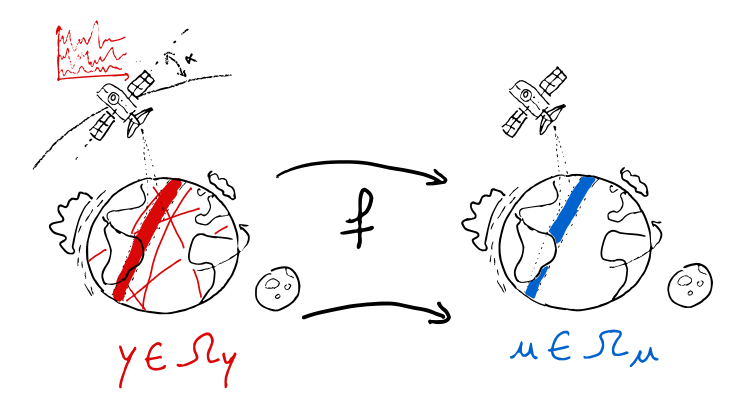
\includegraphics[width=0.8\linewidth]{Chapitre1/Ch1-Figures/Cal_drawing.png} 
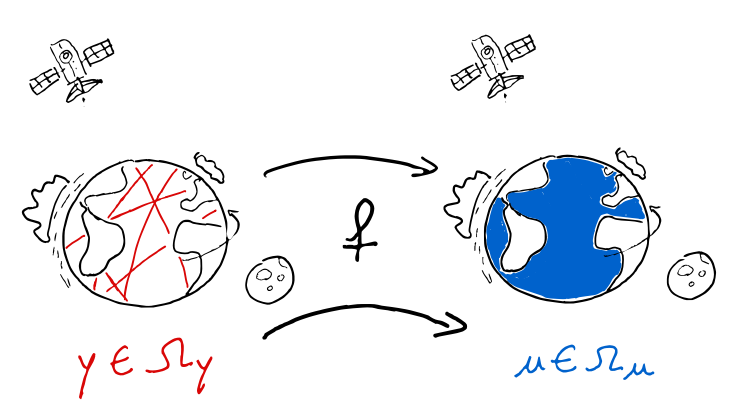
\includegraphics[width=0.8\linewidth]{Chapitre1/Ch1-Figures/Mapping_drawing.png} 
\end{center}
\caption[Swot calibration and altimetry mapping problem illustration]
{\footnotesize The calibration problem (top row) consists in finding the mapping $f$ that estimates the observed SSH $u$ from the SWOT satellite given the actual noisy measurement and ancillary calibrated measures ($y$).
The mapping task (bottom row) consist in finding an operator $f$ that maps partial measurements of the SSH $y$ to a map of SSH $u$}
\label{fig:planet_drawings}
\end{figure}


% \begin{figure}[htbp]
% \begin{center}
% \begin{tabular}[c]
% 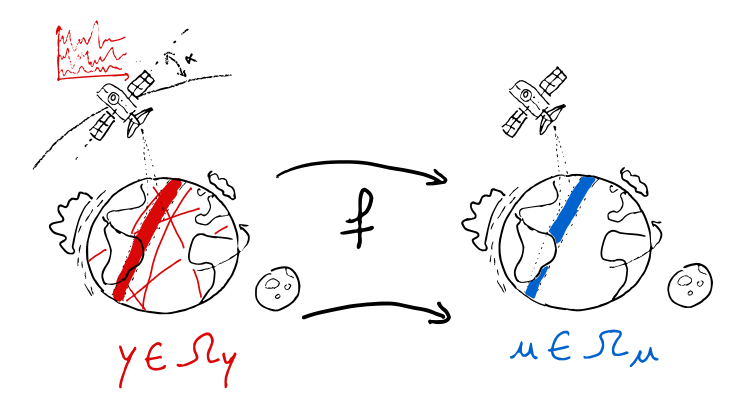
\includegraphics[width=0.8\linewidth]{Chapitre1/Ch1-Figures/Cal_drawing.png} \\
% 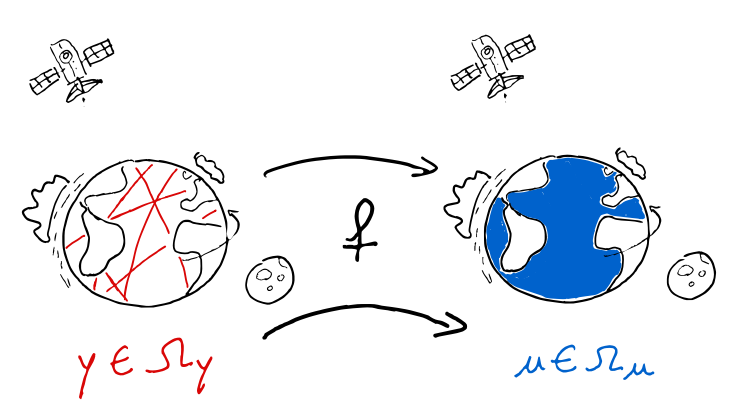
\includegraphics[width=0.8\linewidth]{Chapitre1/Ch1-Figures/Mapping_drawing.png} \\
% \end{tabular}
% \end{center}
% \caption[Swot calibration and altimetry mapping problem illustration]
% {\footnotesize The calibration problem (top row) consists in finding the mapping $f$ that estimates the observed SSH $u$ from the SWOT satellite given the actual noisy measurement and ancillary calibrated measures ($y$).
% The mapping task (bottom row) consist in finding an operator $f$ that maps partial measurements of the SSH $y$ to a map of SSH $u$}
% \label{fig:planet_drawings}
% \end{figure}

\begin{figure}[htbp]
\begin{center}
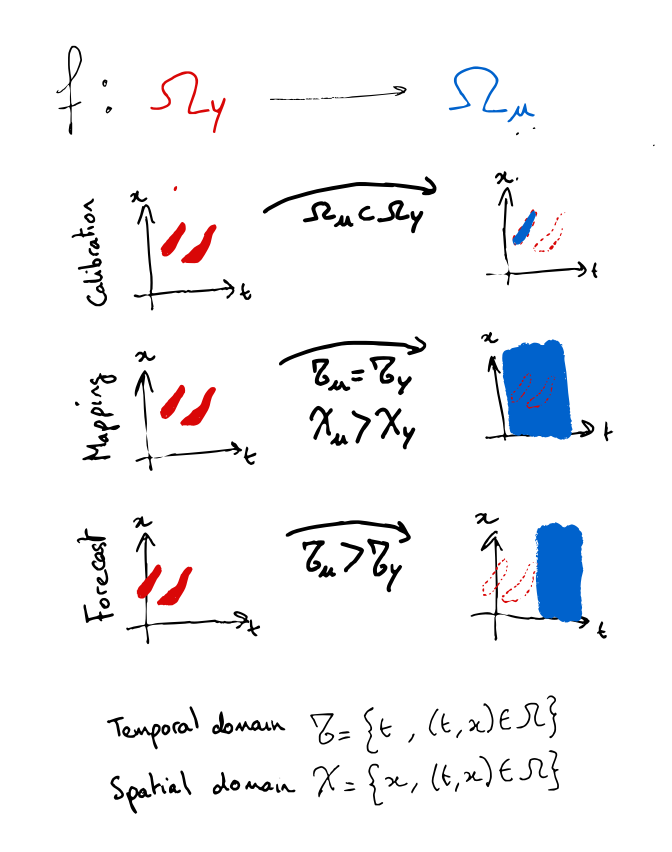
\includegraphics[width=0.8\linewidth]{Chapitre1/Ch1-Figures/Task_ontology.png}
\end{center}
\caption[Task characterization through the domains $\Omega_u$ and $\Omega_y$ of $u$ and $y$]
{\footnotesize Using the perspective provided by the problem definition, we can easily categorize earth observation problems.
The calibration consist of estimating the field $u$ on a subset of the observation domain, the mapping consist in estimating $u$ on the same temporal domain but extending the spatial domain.
And finally forecast can considered as wanting to estimate a quantity on an unobserved future domain.}
\label{fig:task_ontology}
\end{figure}

\section{Method Ontology}
We aim to characterize and organize the various methods used to tackle the class of problem introduced in \ref{sec:chap1_problem_form}. We propose that all methods can be decomposed into the following two steps:
\begin{itemize}
\item Step 1: Define the set $\cal{F}$ of possible $f$ using theoretical knowledge (conceptual models)
\item Step 2: Search $\cal{F}$ for an optimal $f$ using factual knowledge (data)
\end{itemize}

To illustrate our point, consider a simple example of building a thermometer by placing a liquid in a tube and wanting to interpret the level of the liquid as a temperature. According to our previous notations, $y$ is the level of the liquid and $u$ is the temperature of the liquid inside, and we seek to find the mapping $f$ between the two.

Step 1 involves compiling our theoretical knowledge on the problem to define the class of function. Given our understanding of fluid dilation in response to temperature, under the assumption that the diameter of the tube is constant with height, we can state that the level is linearly correlated with the temperature. Therefore, $f$ will be part of $\cal{F} = { y: \alpha y + \beta , (\alpha, \beta) \in |R^2 }$.

In Step 2, to find $\alpha$ and $\beta$, we require two data points to calibrate our model, traditionally obtained by placing the thermometer in icy and boiling water at 1 bar of pressure to get the levels corresponding to 0°C and 100°C. This method relies on strong theoretical foundations and assumptions to reduce the dimensionality of the search space $\cal{F}$, thus facilitating the parameter search with relatively few data points.

However, if we clearly see that the diameter of our thermometer is not constant, the model needs to incorporate that the evolution of the temperature depends on the diameter at each height. This expands the class of functions, necessitating the incorporation of a model of the evolution of the diameter in function of the height, which will introduce new parameters. We could assume that the diameter is linear for every 5mm section, and the corresponding parameters to search would be the value of the diameter every 5mm.

To estimate these new parameters, we need more data which could be direct measures of the diameter or measures of temperature every 5mm. We could directly model $f$ as linear per part, thereby reducing the number of parameters to estimate (no more $\alpha$ and $\beta$). If we have measurements of the temperature, this also alleviates the need to explicitly model the relationship between diameter and temperature.




  
% Tasks
% Simple exemple
% Calibration and mapping example

% Tasks of interests can be summed up as finding f
% Finding f takes two steps: defining the set of possible fs, searching the set for the best f
% Formulating the sets of F requires theoritical knowledge
% Searching the sets of F requires data

% From theory to sets of 
%   inverse problems state x
%   data assimilation: dynamical model
%   spatio temporal correlation: Covariance model
%   deep learning
%   locality: convolution
%   temporal dependence RNN LSTM


Lorem ipsum dolor sit amet, consectetuer adipiscing elit. Maecenas fermentum, elit non lobortis cursus, orci velit suscipit est, id mollis turpis mi eget orci.

\section{Première section du chapitre}

Lorem ipsum dolor sit amet, consectetuer adipiscing elit. Maecenas fermentum, elit non lobortis cursus, orci velit suscipit est, id mollis turpis mi eget orci.

\subsection{Première sous-section}

Lorem ipsum dolor sit amet, consectetuer adipiscing elit. Maecenas fermentum, elit non lobortis cursus, orci velit suscipit est, id mollis turpis mi eget orci.

Voir figure \ref{fig:mafigure2}.


\begin{figure}[htbp]
   \begin{center}
      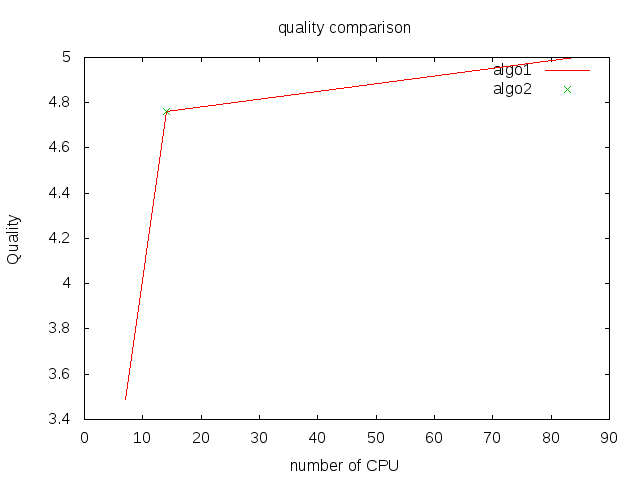
\includegraphics[width=0.8\linewidth]{Chapitre1/Ch1-Figures/comparison.png}
   \end{center}
   \caption[titre court pour la liste des figures]
   {\footnotesize Titre plus long avec des explications.}
   \label{fig:mafigure2}
\end{figure}

\subsection{Deuxième sous-section}

Lorem ipsum dolor sit amet, consectetuer adipiscing elit. Maecenas fermentum, elit non lobortis cursus, orci velit suscipit est, id mollis turpis mi eget orci.

\section{Conclusion du premier chapitre}

Lorem ipsum dolor sit amet, consectetuer adipiscing elit. Maecenas fermentum, elit non lobortis cursus, orci velit suscipit est, id mollis turpis mi eget orci.

In this manuscript I'd like to cite \cite{remo3,remo4}.

\addcontentsline{toc}{section}{Bibliography}
\putbib[./Chapitre1/Ch1-Biblio.bib]
\end{bibunit}

\clearemptydoublepage
\begin{bibunit}[IEEEtran.bst]

  \chapter*{First and second order modeling for altimetry problems}
\addcontentsline{toc}{chapter}{First and second order modeling for altimetry problems}
  \chaptermark{First and second order modeling for altimetry problems}
 
 Exsisting approaches for modeling alitmetry problems.
 Goal estimate the SSH on a continuous spatio-temporal domain $\Omega_u$
 
 
  \section{Priors: Chosing a model of the SSH}
A first step is to compile our theoritical knowledge into some assumptions 

 
  \subsection{State representation}
A first decision needs to be a choice on the representation of this SSH field on this domain. For example, if $\Omega_u$ is a 10°x10° over a year. A example representation would be values of SSH every 1/10° and 24h. Such a representation will discard some small processes and introduce model error.
This define the state that to estimate

 Grid representation
     - ssh values at regular sampling dx, dt
     - ssh values at t0
     - ssh and ancillary variable values
     - ssh decomposition (multiscale, wavelet)
  functional representation
     - Nerf parameters

  through other signals:
      in calibration the SSH is defined like everything that is not roll,timing,phase...
      
  \subsection{SSH estimation from state}
This state representation is couple with a function that maps state values to SSH values 
This choice will also impact the final SSH estimation, given grid representation of the SSH, the interpolation choice for estimating values inbetween grid points will give different results
In 4DVar the dynamical model used to propagate the initial conditions will give different trajectories
In nerf the neural architecture chosen 


  \subsection{Prior costs}
A final way is to define a score over the state space to characterize which 
This can be done trough likely estimation and error covariance matrices, energy based neural estimation




| Method              | state repr                         |          state -> ssh           |                            prior cost                             |
| ------------------- |:---------------------------------- |:-------------------------------:|:-----------------------------------------------------------------:|
| OI                  | Grid $x$                           |             interp              |                          $\|x - x_b\|_B$                          |
| s4DVar              | Grid t0 $x_0$                      |          dyn model  ++          |                         $\|x_0 - x_b\|_B$                         |
| w4DVar              | Grid                               |             interp              | $\|x - x_b\|_B + \sum\|x_{k+1} - \cal{M}_{k\to k+1}(x_k)\|_{Q_k}$ |
| MIOST               | wavelet $x$    +                   |      wavelet transform   +      |                  $\|x - x_b\|_{\Gamma Q\Gamma}$                   |
| 4DVarNet            | 2 scale Grid $x =(u_{ss}, u_{ls})$ | $u = u_{ss} + u_{ls}$,   interp |                     $\|z - \Phi_{NN}(z)\|_B$                      |
| Nerf                | NN Params                          |        NN inference +++         |                               None                                |
| Direct NN inversion | Grid                               |             interp              |                               None                                |



  \subsection{Solvers: Estimating the state given some observations}

Once all prior assumptions about the SSH field have been made, the next choices concern the **calibration procedure** used to estimate the state given some observations.

This requires formulating about the relationship from the observations to the state and chosing an estimation procedure.


A class of method start by defining an observation operator $H$ that describe how to go from state to observations, finding $f$ consist in finding the inverse of this operator $H$. This class of method is named "inverse problem"
This problem is usually ill posed, without a unique solution.
Using a grid representation of the SSH without other prior will only allow to fill the observed pixels 

$y = H(x) = \cal{H}(x) + \epsilon$
After making assumptions on $\epsilon$ such as unbiased gaussian noise.
The field of data assimilation in geoscience propose a variety of methods to solve inverse problems.
We can mention here linear algebraic resolution of the kalman gain in Kalman filters and optimal interpolation.
But also variational methods that formulate the estimation as a minimization problem, the objective to minimize is called variational cost and usually include a observation term and a regularization term making use of the prior cost.
The minimization procedure usually involves some kind of iterative gradient based algorithm.



Deep learning also opened the way to directly model the link model the inversion process with a neural network as done in \cite{}. We call this approach direct inversion





| Methods    |         estimation         |   O(y, x)   |
| ---------- |:--------------------------:|:------------:|
| Nerf       | $\theta = argmin(\cal{L})$ |  $\cal{L}$   |
| Var        |      $ x = argmin(\alpha R(z) + \beta O(y, x))$      |    $\|y - Hx\|$          |
| OI, Kalman | $x = x_b + K(y - Hx_b)$ | $\|y - Hx\|$ |
| Direct Inv |          x = f(y)          |              |
            



For nadir altimetry, thanks to the calibration  most methods usually make the assumption of unbiased gaussian noise. 
$\| y - \cal{H}(x)\|_R$ 


## Second order Modeling and estimation }
All those choices of prior on the ssh field, observation cost, estimation procedure introduced new factors that need to be determined.
Those factors include the background field of data assimilation schemes, as well as the error covariances for the observation and background. They include choices within numerical schemes parameter for variational optimization procedure or numerical model integrations.
Finally those factors also include the neural network parameters.

The process estimation of those quantities unfold in a similar manner as the estimation of the SSH.
It relies on available calibration data that are beyond the sole observations of an estimation problem but include numerical model outputs and historical data.

Given the theoritical knowledge at hand, assumptions are made about what distribution is reasonable to model the errors and to how to model the covariances between the errors, what numerical schemes should be considered for integrating the dynamical models, what constitutes a good first guess for data assimilation schemes and so on... What neural architecture is suited for the direct inversion problem.

Those assumptions characterizes the quantities that need to be estimated and we can differentiate multiple ways that are used to determined them.

A combination of different methods are used to estimate those quantities.

Cross validation consists in using part of the calibration data to evaluate the choice, 
The choice can then be made "randomly", through some statistics on the calibration data aor through some optimization procedure (bayesian opt or gradient descent...)

In the case of direct inversion, the search for the neural parameters are equivalent the state search of the nerf method

Note that in some sense second order calibration data also contain information that we would like to infuse to our method, so solving the second order problem is the data centric part of the methodology. 
The information stored in available data can be used to tune the prior models, or the state estimation procedure.
Neural Direct inversion approach virtually has no prior models (except from the state formulation) and all info contained in the data goes only into the estimation procedure.

\section{A closer look on the 4dVarNet}
the 4dvarnet framework was a promising at the time of my thesis with strong performances when evaluated on simulated SSH estimation.
The main use case of interest concerned the interpoaltion task on a 10°x10° region traversed by strong currents from the gulfstream generating dynamic SSH.
The simulated SSH used was from the NATL60 simulation and the altimetry configurations considered were 4 nadir altimeters with and without swot observations
Some version also considered an optimal interpolation of the OI as observations to the mapping problem
We detail below the assumptions made and the different components used.


\subsection{State formulation}
The current 4dvarnet framework uses a grid representation of the SSH at a certain resolution, however a few different variations have been experimented in different work:
some work represent the SSH directly as scalar
other decompose each ssh value in a large and small scale components
finally another formulation consists in introducing latent values in addition to the two scale components 


\subsection{Prior cost}
In the 4dvarnet the prior cost is formulated as an autoencoder loss.
Given a nn $\phi$, $R(x)=\|x - \phi(x)\|$
Some use simple or multiscale bilinear blocks
Some tried with Unets
on simplified lorenz system, the pde of the system has been tested therefore being a 4dvar formulation



\subsection{Observation operator}
Previous work make a no noise assumptions and link directly the observed values to the coresponding grid values
Some work also introduce a multimodal verion making use of sea surface temperature observations that are linked to the state using neural network formulation.


\subsection{State Estimation procedure}
In this work different approaches were considered for  estimating the state.
A fixed point algorithm analog to EM were used by maximizing the obs likelihood (clipping the obs to the state) then making a forward pass with the $\phi$
Other approaches used the variational formulation of minimizing a combination of observation and prior cost


\subsection{Learning: Estimation procedure}
Apart from the cross validation and exploration of different architectures and configurations, the actual parameter values of both the neural solver and the neural prior are trained using a standard deep learning otpimization procedure Adam. There parameter are tune to minimize the mean squared error of the SSH reconstruction as well as  the reconstruction of the gradient. In order to further guide the weights of the neural prior, a term in the training loss is added to nudge the estimated states have low autoencoder loss.

%   \section{First order: Estimating an SSH field}
%
%   First order calibration data is a sample of altimetry observations corresponding to a single estimation task.
%   The estimation can be of a map and the data would be the surrounding nadir observations.
%   The estimation could also be of the calibrated SSH, and then the data would be the concerned nadir track as well as the surrounding nadir observation.
%
%   \subsection{Assumptions about the SSH field: Model and model state}
%   % maybe start with the state, ssh, constraints on state
%   The kind of assumptions we make about the SSH field will result in two components.
%   The definition of a state which will be a set of values to be determined for the SSH estimation as well as some computational procedure to infer the SSH values on the domain from the state.
%   Each choice of model introduce parameters that need to be tuned prior to state inference
%
%   Model -> state -> parameters -> inference
%   Dynamical models of the ocean -> initial conditions (weak constraints: initial condition per subsegment) -> integration grid and step -> integration scheme
%   Grid -> SSH grid values -> resolution -> interpolation
%   Covariance model of errors wrt a first guess -> First guess errors -> addition / interpolation
%   Neural network -> parameters -> architecture -> nn inference
%   Composite signal with additive errors -> error parameters -> 
%   Dimensionality reduction -> basis components
%   Auto-Encoder -> grid -> interpolation (similar to denoising)
%
%
%   \subsection{State estimation procedure}
%     Depending on the prior assumptions, different approaches exists to perform the actual state estimation from the altimetry observations.
%     Each procedure also introduce parameters that need to be tuned for inference.
%
%     cross-validation leaving some calibration data out, trying different values and checking which ones works best.
%     bayesian estimation: kalman gains of kalman filters  and optimal interpolation computation in observation error modeling
%     Variational methods: data assimilation or optimal interpolation solving a minimization problem.  Minimization procedure (iterative step), observation cost
%     Neural network training: Stochastic gradient descent, learning to learn algorithm,  (J em)
%     Neural network inference (for grid values, for covariance matrix) (Manuch)
%
%
%   \section{Second order problem: tuning the parameters of SSH model and estimation procedure}
%   In order to solve the SSH estimation tasks, the parameters introduced in the model and estimation procedure need to be determined.
%
%
%   The calibration data for this second order data represent historical observations as well as potential numerical simulation
%   Some parameters can be estimated through statistical analysis of historical data when available.
%   the first guess can be determined through historical average
%   noise levels can be informed by historical data and tuned through different 
%
%   Others need to be calibrated on similar tasks that can be evaluated on OSE or OSSE setup.
%   Neural network parameters can be trained
%   Sensible grid and integration schemes of dynamical model can be chosen
%   Covariance matrices 
%
%
%   Note that the second order calibration can introduce hyper parameters than themselves need to be determined,
%   they are usually found through trial and error in a cross validation  fashion.
%
%
% \section{A closer look at the 4dVarNet prospect: a hybrid approach}
%   \subsection{overview}
% This thesis is extensively on prior work 
% This 4dVarNet makes an interesting combination of classical and deep learning based methods.
% The first order assumptions made on the SSH field is that the field should be a fixed point of a certain neural network phi.
% the state is represented as a spatial temporal grid, first application decompose the ssh value in a large scale and small scale component.
% this phi can be though as analoguous as the integration of the dynamical model in strong 4DVAR, in which want the estimated SSH to be the integration of the 
% in order to find the state that satisfy the prior for given observations, a variational formulation is employed,
%   meaning that the estimation is done trhough the minimization of a quantity.
%   This minimization is done using a neural based gradient descent initially developped for meta learning tasks involving a recurrent neural network
%   The second order parameters therefore consists in the neural network parameters of the phi operator as well as the parameters of the recurrent neural network.
%
% \subsection{Existing results}




  
%   \chapter*{Model driven, data-driven and deep learning for altimetry analysis.}
% \addcontentsline{toc}{chapter}{Deep Learning, inverse problems and altimetry}
%   \chaptermark{Model driven, data-driven and deep learning for altimetry analysis.}
%
%
%
%
% As presented in the previous chapter, the \textbf{model} and \textbf{calibration data} are inter-dependent. The number of parameters of the model will impose constraints on the quantity calibration data and reciproquely the available data will constrain the kind of model that can be considered.
% This coupling introduce a possible distinction between model-driven and data-driven approaches. We use this distinction to organize the overview of the existing altimetry methods in the first two sections.
% Deep learning can be viewed as data-driven but introduce specific considerations that are presented in a third section.
%
%
%   \section{Model driven}
% We designate by model-driven the class of methods that are predicated on domain specific assumptions.
% \subsection{Data assimilation for altimetry: mapping}
% The ocean being a dynamical system, we look more in detail about the methods making use of physical assumptions of the system in the form of dynamical models.
%
% We will first detail here more precisely the data assimilation methods that leverage dynamical knowledge of ocean processes for altimetry mapping.
% In geoscience, data assimilation refer to the estimation of a state $X$ from observation data $y$ using a dynamical model $M$.
%
% In practice, data assimilation work in altimetry rely on \textbf{models} that vary greatly in complexity.
%   The reanalysis GLORYS12 rely on the full-fledged Ocean General Circulation Model (OGCM) NEMO\cite{} which solves the primitive equations and models the sea-ice.
%   Other works rely on simplified Quasi-Geostrophic dynamics.
%
%
%   Given a dynamical model, different formulation and algorithms are used to assimilate the observation data.
%   We detail three methods which are Kalman filtering\cite{}, Variational data assimilation\cite{} and back and forth nudging\cite{}.
% Kalman filtering is a sequential assimilation method that requires a linearization of the dynamical model and the observation model and assume gaussian noise in the observation and the model.
%   This principle is at the base of the SEEK formulation used for state of the art operational oceanography like product like Glorys.
%   Variational data assimilation (VarDA) formulates the problem as a minimization problem in which the state minimizes an observation discrepency cost combined with a regularization cost involving a dynamical integration of the state.
%   The minimization of the variational cost then involves an iterative optimization procedure like a gradient descent.
%   Flavours of VarDA go from 3DVAR, 4DVAR, weak4DVAR. 3D-Var is also used for biais correction in GLORYS12 product\cite{}. Variational approaches do not require the model to be linear but the optimization procedure can be computationally expensive by requiring multiple integrations of the dynamical model.
%   Back and forth nudging (BFN) is an approach that has been succesfully used to assimilate altimetry data with a QG model\cite{}. It can be seen like an hybrid method between kalman filtering and VarDA and consists in iteratively integrating the model forward and backward in time while adding a term to the dynamical model that nudges the integration towards observed values. 
%
% \subsection{Systematic error modeling for SWOT calibration}
% For the SWOT calibration of correlated errors, fewer studies exists. However envisionned operational approaches also rely on models, but instead of modeling ocean processes, they model the processes behind the error signals.
% Once the different processes are modeled, calibration data is used to estimate the parameters of the error processes.
%
% \section{Data driven}
% Data driven aims at making the minimal assumptions given the available data, the problem can then be seen as an interpolation problem. 
% Optimal interpolation is the main method used in altimetry. The model characterizes  the spatial and temporal decorrelation rate through a covariance model.
% parameters covaraince model as well as decorrelation factor.
% covariance can depend on place and time
%   MIOST solve in reduced wavelet basis, the choice of basis adds additional parameters.
%
%
% \section{deep learning}
% Deep learning models are data driven but require potentially even less
%   deep learning models for computer vision are mostly based on convolution filters and non linearities.
%   deep learning calibration algorithms include stateful gradient descent with adaptive step size and second order term estimation that can themselfes be parameterized with neural networks.
%
%   Application of deep learning for altimetry has known a significant boom during the course of this PhD.
%   Traditional CV architectures have been tested on QG simulation with toy spatial and temporal interpolation tasks.
%   the 4dvarnet inspired from variational data assimilation tested in  OSSE with a SOTA simulation.
%   by the end of the thesis, ConvLSTM have been trained on real altimetry data.
%
%   For the calibration of swot, studies exist to remove the KaRIN noise but not for the correlated errors.
%
%





% We aim here at providing a more detailed overview of the state of the art methods for tackling the mapping and calibration challenges adressed in following chapters.
% First we introduce the generic class of inverse problems.
%
%
%
% Denoising. Reconstructing the trajectory of a dynamical system from observation.
%
% One characteristic of such problem is that they are usually ill-posed, in the sense that the solution may not be unique.
% Different approaches for solving these inverse problems rely on different way to model the sytem and computational methods to estimate the parameters of the system from the data.
% Therefore inverse problem solving methods usually rely on injecting prior knowledge about the system in the model.
%
% We'll first look in detail at two different method
% Tasks such as altimetry mapping and SWOT calibration have both been adressed before.
%   In this chapter we review the formalism and methods that exists for solving such problems.
%   Both task can be formulated as inverse problems, and this chapter is organized as follows:
%   First part will look 
%   Given some data $y$ that result from a process $\cal{F}$ applied to some state $x$, the task of determining $x$ from $y$ can 
% Estimating an underlying state from a 
% The task we introduced can be seen as inverse problems and existing 
% We have introduced in the previous chapter the different components to consider when addressing observation problems such as altimetry mapping and calibration. In this chapter, we'll paint the landscape of the different approaches that have been developped in order to contextualize where our research fit in.
%
%
%
%
% Observation tasks such as altimetry mapping and sensor calibration can be seen as inverse problems. 
% Inverse problems broadly encompasses the tasks of estimating states parameters of a system from data produced by that system.
% These problems are characterized by their ill-posedness. 
% Over the years different class of computational methods have been developped to solve these problems. Recently deep learning has also been increasingly used for such problems.
% We detail in the first section of this chapter how the altimetry usecases considered fit in the inverse problem formulation justifying therefore the relevance of this category of methods.
% In the second section we present two state of the art domain approaches that are especially relevant for our case.
% In the third section, we present the deep learning methods 
%   Finally we'll describe the 4dvarnet, a neural scheme inspired by variational data assimilation
%
%   \section{Altimetry Usecases as inverse problems}
%   \subsection{Notation for inverse problems}
%
%   \subsection{Mapping methods}
%   \subsection{Calibration Methods}
%
%   \section{Domain methods for Inverse Problems}
%   \subsection{Model driven: Dynamical prior and data assimilation}
%   \subsection{Data driven: Statistical prior and optimal interpolation}
%   \subsection{Experimental methods }
%
%
%   \section{Deep learning for inverse problems}
%   \subsection{Deep prior and neural radiance fields}
%   \subsection{Direct inversion}
%   \subsection{Physics informed deep learning}
%
%
%   \section{An hybrid method: the 4dVarNet}
%
%
%
%
%   \begin{itemize}
%     \item OI
%     \item MIOST
%     \item DYMOST
%     \item DA (Kalman filters, 4DVAR)
%     \item convlstm
%     \item Dincae
%     \item 4dVarNet
%   \end{itemize}
% \section{Models}
%   \subsection{Physics}
%   \begin{itemize}
%     \item Ocean physics BFN, GLORYS 
%     \item Calibration roll estimation
%   \end{itemize}
%   \subsection{Statistics}
%   \begin{itemize}
%     \item OI
%   \end{itemize}
%   \subsection{Deep learning}
%   \begin{itemize}
%     \item 
%   \end{itemize}
% \section{Data}
%   \subsection{Observations}
%   \begin{itemize}
%     \item 
%   \end{itemize}
%   \subsection{Numerical model simulations}
%   \begin{itemize}
%     \item 
%   \end{itemize}
% \section{Algorithm}
%   \subsection{Statistics}
%   \begin{itemize}
%     \item 
%   \end{itemize}
%   \subsection{Data Assimilation}
%   \begin{itemize}
%     \item 
%   \end{itemize}
%   \subsection{Iterative Gradient based}
%   \begin{itemize}
%     \item 
%   \end{itemize}
% \section{Evaluation}
%   \subsection{OSSE}
%   \subsection{OSE}
%
%
%
%
% Section 1: Altimetry Usecases as Inverse Problems
% Introduction
%
% Altimetry, particularly when it involves oceanic applications, often deals with indirect measurements. Essentially, we have observable data—like sea surface height—from which we aim to estimate underlying physical states or parameters, such as current velocities or sea bed topology. This task fits squarely within the framework of what are called 'inverse problems'.
% Notation for Inverse Problems
%
% Before we delve into the specifics, let's set some simple notation to help us along the way:
%
%     yy: Observed data (e.g., sea surface height)
%     xx: Parameters or states to be estimated (e.g., ocean currents)
%     FF: Forward model that connects xx to yy, F(x)=yF(x)=y
%
% The goal of an inverse problem is to find xx given yy and FF.
% Mapping Methods
%
% Ocean altimetry mapping aims to derive high-resolution ocean surface topography or currents from relatively sparse and irregularly distributed satellite altimetry data. These methods take the observable—sea surface height (yy)—and use it to estimate underlying physical states like ocean currents (xx) using a forward model FF that incorporates equations of fluid dynamics and other physical laws. These are quintessential examples of inverse problems.
%
% In the literature, techniques like Optimal Interpolation and Kalman Filtering have been extensively used for this task. These methods come with their own assumptions and limitations, such as requiring the error statistics to be Gaussian or assuming linearity in the forward model FF.
% Calibration Methods
%
% Calibration in the context of altimetry involves adjusting sensor parameters to ensure that the measurements are accurate and reliable. Here, the observed data (yy) could be the raw readings from the altimeter, and the states or parameters (xx) would be the calibration factors. The forward model FF in this case would describe how the calibrated sensor should behave under ideal conditions.
%
% For example, one might have a mathematical model FF that predicts sensor readings based on laboratory conditions and known physical laws. The inverse problem then is to adjust xx (calibration parameters) such that F(x)F(x) closely matches yy (actual sensor readings).
%
%
% Section 2: Domain Methods for Inverse Problems
% Introduction
%
% The landscape of computational methods for solving inverse problems in altimetry is quite diverse. Broadly, these methods can be classified into three categories: model-driven, data-driven, and experimental methods. Each has its advantages and limitations, and the choice often depends on the specific use-case, data availability, and computational resources. This section aims to provide an overview of these classes of methods, particularly in the context of ocean altimetry.
% Model-Driven: Dynamical Prior and Data Assimilation
% Definition
%
% Model-driven methods often employ a priori knowledge of the physical laws governing the system. In oceanography, this could involve fluid dynamics, gravitational forces, and thermodynamics to make educated estimations. Data assimilation techniques, such as the Kalman filter, are typical examples.
% Pros and Cons
%
%
% Data-Driven: Statistical Prior and Optimal Interpolation
% Data-driven methods rely on statistical models to solve inverse problems. Rather than using detailed physics-based models, these methods use statistical approaches to approximate the relationship between observed data and underlying states. Optimal Interpolation is a commonly used technique.
%
%
% Experimental methods:
% BFNQG
% MIOST
% DYMOST

\end{bibunit}


\clearemptydoublepage
% \documentclass[lettersize,journal]{IEEEtran}
% \usepackage{amsmath,amsfonts}
% \usepackage{algorithmic}
% \usepackage{array}
% \usepackage[caption=false,font=normalsize,labelfont=sf,textfont=sf]{subfig}
% \usepackage{textcomp}
% \usepackage{stfloats}
% \usepackage{url}
% \usepackage{verbatim}
% \usepackage{graphicx}
% \usepackage{booktabs}
% \usepackage{pgfplots}
% \usepgfplotslibrary{external} 
% \usepackage{layouts}
% \hyphenation{op-tical net-works semi-conduc-tor IEEE-Xplore}
% \def\BibTeX{{\rm B\kern-.05em{\sc i\kern-.025em b}\kern-.08em
%     T\kern-.1667em\lower.7ex\hbox{E}\kern-.125emX}}
% \usepackage{balance}
% \begin{document}
% \title{Scale-aware neural calibration for wide swath altimetry observations}

% \author{Quentin Febvre, ~\IEEEmembership{Student,~IEEE,} Clément Ubelmann, Julien Le Sommer, Ronan Fablet%
% \thanks{Quentin Febvre and Ronan Fablet are with IMT Atlantique and UMR CNRS Lab-STICC, INRIA team Odyssey, Brest, France. Email: quentin.febvre@imt-atlantique.fr, ronan.fablet@imt-atlantique.fr}%
% \thanks{Clément Ubelmann is with Datlas, Greno, France. Email: clement.ubelmann@datlas.fr}
% \thanks{Julien Le Sommer is with MEOM group at Université Grenoble-Alpes, CNRS, IRD, Grenoble, France. Email: julien.lesommer@univ-grenoble-alpes.fr}}

% \markboth{Transactions on geoscience and remote sensing}%
% {Scale aware deep learning for wide-swath altimetry calibration}


% \maketitle
\begin{bibunit}[IEEEtran.bst]

\clearemptydoublepage
% \chapter{Scale-aware neural calibration for wide swath altimetry observations}
  \chapter*{Scale-aware neural calibration for wide swath altimetry observations}
\addcontentsline{toc}{chapter}{Scale-aware neural calibration for wide swath altimetry observations}
  \chaptermark{Scale-aware neural calibration for wide swath altimetry observations}

  
% \begin{abstract}
% 	Sea surface height (SSH) is a key geophysical parameter for monitoring and studying meso-scale surface ocean dynamics. For several decades, the mapping of SSH products at regional and global scales has relied on nadir satellite altimeters, which provide one-dimensional-only along-track satellite observations of the SSH.  
% 	The Surface Water and Ocean Topography (SWOT) mission  deploys a new sensor that acquires for the first time wide-swath two-dimensional observations of the SSH. This provides new means to observe the ocean at previously unresolved spatial scales. A critical challenge for the exploiting of SWOT data is the separation of the SSH from other signals present in the observations. In this paper, we propose a novel learning-based approach for this SWOT calibration problem. It benefits from calibrated nadir altimetry products and a scale-space decomposition adapted to the structure of the different processes in play in the SWOT's swath geometry.
% 	In a supervised setting, our method reaches the state-of-the-art residual error of $\approx$ 1.4cm while proposing a correction on the entire spectral from 10km to 1000km and using weaker constraints on the modeled error signal.
% \end{abstract}

% \begin{IEEEkeywords}
% Deep Learning, Altimetry, Calibration, SWOT.
% \end{IEEEkeywords}


\section{Preface}
The first chapter aims to assess the potential of deep learning models in addressing altimetry challenges. Specifically, we focus on the task of cross-calibrating SWOT correlated errors using calibrated NADIR observations. This scenario serves as a compelling use case for evaluating the potential of deep learning in altimetry data analysis since it involves considerations related to both the ocean system and the observing system. Additionally, the successful utilization of SWOT data hinges on the removal of error signals, introducing a novel sensor into the equation.

The deep learning solution presented here leverages existing mapping methods to provide an initial estimate of SSH (Sea Surface Height) on the SWOT swath. It also incorporates a neural network inspired by computer vision architectures to refine this initial estimate using SWOT observation data. Our study demonstrates that incorporating a priori knowledge about error signals when designing the deep learning model is crucial for improving the initial estimate.

To evaluate our proposed approach, we circumvent the challenges posed by the lack of precise knowledge regarding SSH and error signals. Instead, we utilize data from state-of-the-art ocean simulations and SWOT error models to calibrate and assess the effectiveness of our method. This approach creates an idealized setup for calibration and evaluation purposes, allowing us to focus on selecting a deep learning architecture suited for the altimetry task. However, it also raises questions about the transferability of deep learning techniques developed in simulated environments to real altimetry data.

\section{Introduction}

Nadir altimeter satellites provide invaluable direct measurements of the sea surface height (SSH) to monitor sea surface dynamics. 
They have played a key role in better understanding ocean circulation and improving climate monitoring. Altimeter-derived SSH data are also of key interest for offshore activities, marine pollution monitoring or maritime traffic routing among others. 

However due to the sparse and irregular sampling associated with nadir altimeter constellations, a wide range of ocean processes from the mesoscale to the submesoscale range remains unresolved, typically for horizontal scales below 150 kilometers and time scales below 10 days. 
The recently launched SWOT mission, with its Ka-band radar interferometer (KaRIn) sensor, provides for the first time higher-resolution and two-dimensional snapshots of the SSH. Once this data is adequately processed, it will likely strongly impact our ability to observe and study upper ocean dynamics \cite{Peral_Esteban-Fernandez_2018}. 

\begin{figure}[!t]
    \begin{center}
        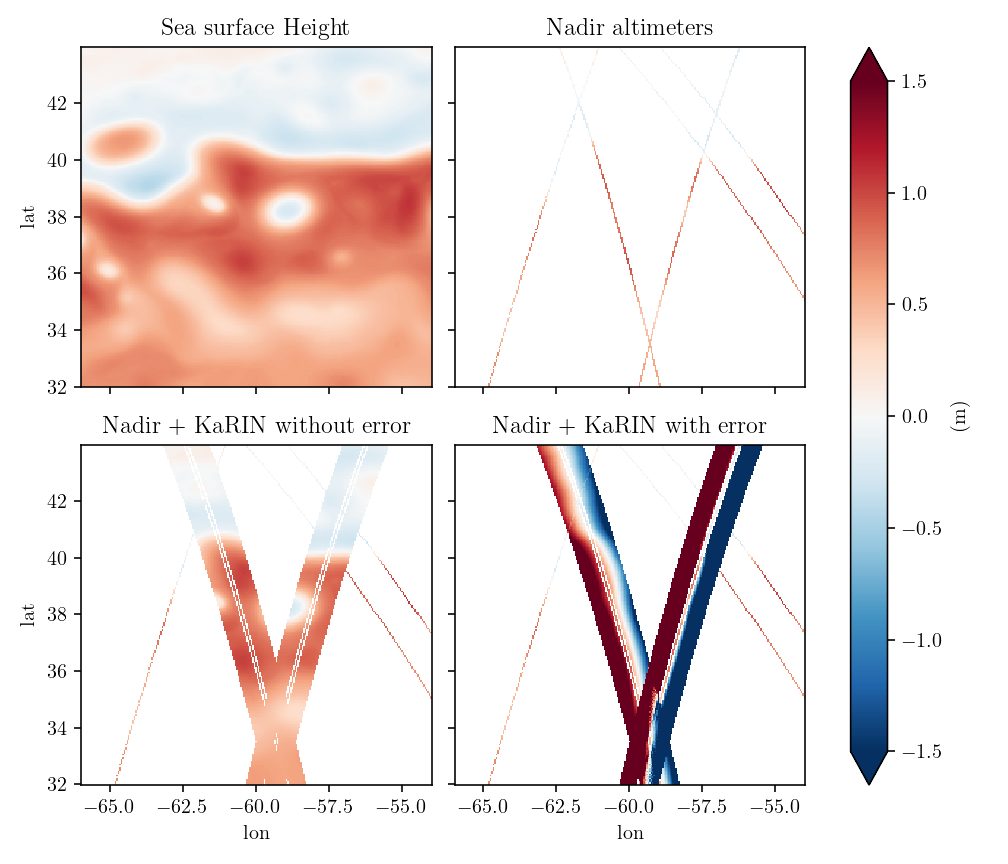
\includegraphics[width=\linewidth]{00_Calib/gridded_sensors.png}
    \end{center}
    \caption{\textbf{Observing System Simulation Experiment Cross-Calibration data:} \textit{Top left:} Sea surface height (SSH) on October 26th 2012 from NATL60 simulation dataset. \textit{Top right:} Calibrated NADIR pseudo-observations sampled using realistic orbits from the SSH, they are used to compute the gridded product for the cross-calibration.\textit{Bottom-left:} NADIR + noise-free-KaRIn pseudo-observations, the  2{\sc d} sampled SSH is the target of the cross-calibration.\textit{Bottom-right:} NADIR + noisy-KaRIn pseudo-observations, simulated errors added to the swath SSH constitute the uncalibrated input of the cross-calibration problem}
\label{c3fig:gridded}
\end{figure}

As reported in Figure \ref{c3fig:gridded}, KaRIn data will be affected by instrument and geophysical errors  \cite{ubelmann_swot_nodate} and their exploitation requires to develop robust calibration schemes. We illustrate in Fig.\ref{c3fig:filtered_swath_uncal_comp} the two main error sources: instrument errors, especially roll errors, are expected to cause the dominant large-scale signal in both across-swath and along-swath directions; and geophysical errors, in particular due to wet-troposphere-induced delays\footnote{We refer the reader to Section \ref{c3subsec:altimetry} for the description of these error signals in raw KaRIn observations.}.
The amplitude of these errors typically range from a few centimeters to a few meters in simulation, when the variability of the SSH for scales below 150km typically amounts to centimeters (See Fig. \ref{c3fig:gridded_impact}). This makes SWOT calibration a particularly challenging task in terms of signal-to-noise ratio. State-of-the calibration schemes \cite{Dibarboure_Ubelmann_Flamant_Briol_Peral_Bracher_Vergara_Faugere_Soulat_Picot_2022} rely on explicit spectral priors to address the calibration problem. 
The underlying hypotheses that one can linearly separate the SSH and the different error components may however impede the performance of such calibration methods. Here, we propose a novel learning-based approach. 
We leverage the computational efficiency of deep learning schemes with a scale-space decomposition \cite{Witkin_1984} adapted to the geometry of KaRIn observations. 

Our main contributions are as follows:
\begin{itemize}
\item{We state the cross-calibration of KaRIn altimetry observations as a learning problem using both raw KaRIn altimetry data and a gridded altimetry product as inputs to the neural network.}
\item{Our neural network architecture applies a scale-space decomposition scheme in the geometry of the KaRIn swath to improve the separability of the SSH and of the errors.}
\item{Numerical experiments using an Observing System Simulation Experiment (OSSE) demonstrate the relevance of the proposed approach and highlight the impact of the quality of the gridded altimetry product to retrieve finer-scale patterns in the calibrated KaRIn observations.}
\end{itemize}
This paper is organized as follows. Section \ref{c3sec:background} provides some background on related work. We introduce the considered data and case-study in Section \ref{c3sec:case_study}. 
Section \ref{c3sec:method} presents our method and we report numerical experiments in Section \ref{c3sec:results}. 
Section \ref{c3sec:conclusion} discusses further our main contributions.

\section{Background}
\label{c3sec:background}
\noindent
\begin{figure*}[!t]%
   \centering
    \subfloat[$f$]{{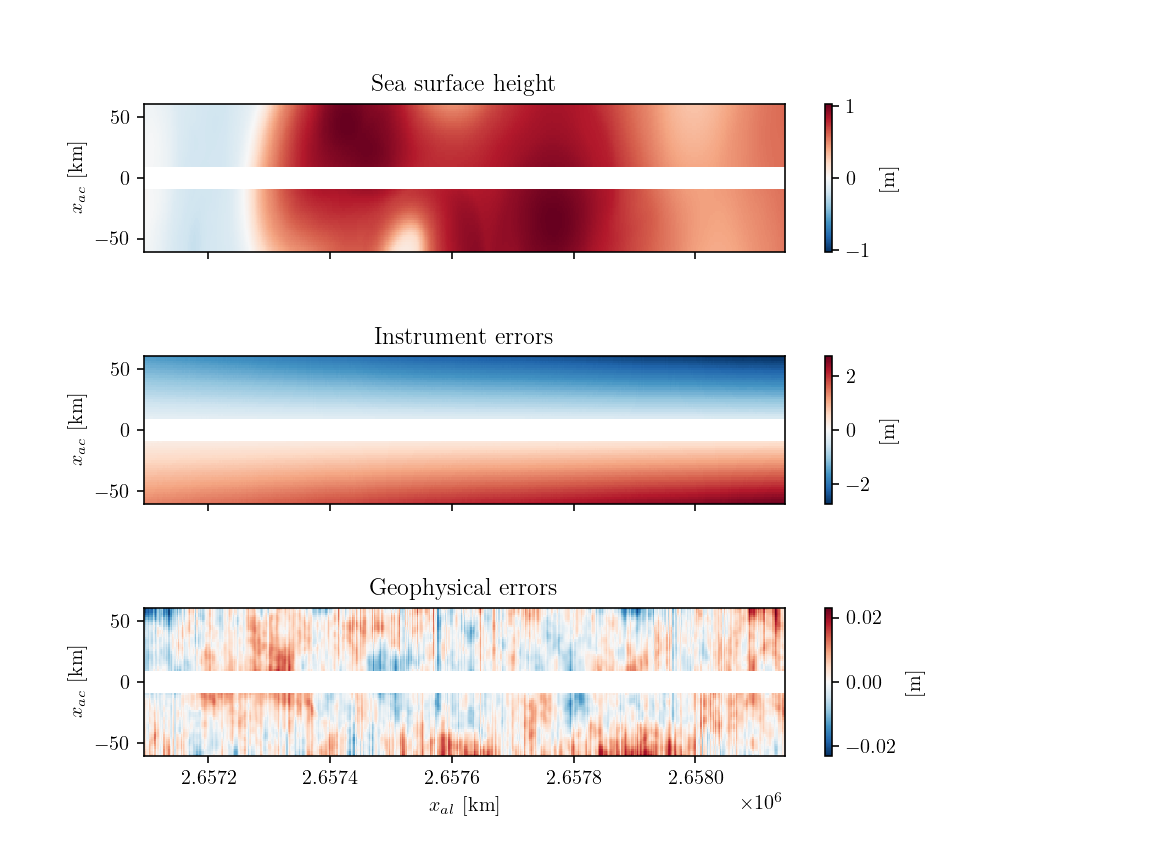
\includegraphics[width=.49\textwidth]{00_Calib/swath_err_details} }}%
    \subfloat[$\mathcal{G}_{200km}(f) - \mathcal{G}_{10km}(f)$]{{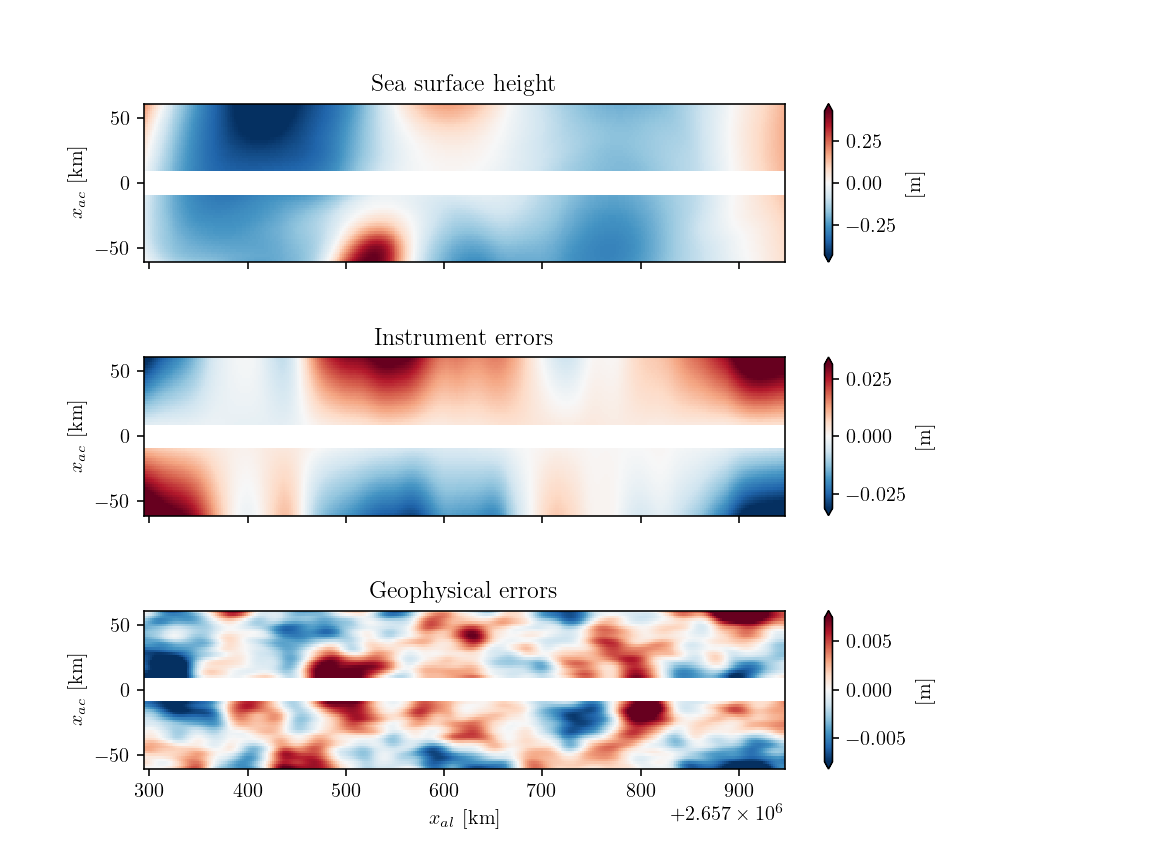
\includegraphics[width=.49\textwidth]{00_Calib/swath_err_f10_200_details} }}%
    \caption{\textbf{1000km segment of KaRIn observation components in swath geometry:}\textit{(a)} Looking at the three signals we see that the large scale instrument errors (middle) are predominant compared to the SSH (top) and geophysical error (bottom). \textit{(b)} Looking at the along-track scales between 10km and 200km, we note that the SSH is dominant w.r.t the error signals.}%
    \label{c3fig:filtered_swath_uncal_comp}%
\end{figure*}
\subsection{Satellite altimeters}
In this paper, we address the cross-calibration of KaRIn observations, meaning that the proposed calibration scheme relies on external calibrated data. More specifically, we consider a constellation of  4 nadir satellite altimeters. We recall that nadir altimeters provide can provide calibrated measurements of the SSH for medium to large scales along 1{\sc d} profiles corresponding to satellites' orbiting paths. Over the last decades the constellation counted typically from 4 to 7 satellites.

By contrast, according to the mission's error budget specification \cite{Peral_Esteban-Fernandez_2018} the KaRIn instrument samples a two-dimensional swath of approximately 120km-wide with a 2km$\times$2km pixel resolution everywhere over the ocean.


In Figure \ref{c3fig:gridded}, we report simulated altimetry observations for both nadir altimeters and KaRIn along with the reference SSH issued from a numerical simulation dataset (see  the Section \ref{c3sec:case_study} for details). As an illustration of the complexity of calibration problem, the error signals completely occlude the SSH signal in the uncalibrated KaRIn observation.
Figure \ref{c3fig:filtered_swath_uncal_comp} illustrates further this point in the swath geometry. When focusing to along-track scales between 10km and 200km, the SSH signal becomes the main signal (Fig. \ref{c3fig:filtered_swath_uncal_comp}). This supports
both to consider a scale-space decomposition and to 
investigate a cross-calibration approach with
the exploitation of nadir-altimeter-derived altimetry products, which typically resolve horizontal scales above 100 km.


\subsection{Interpolation of satellite-derived altimetry data}
\label{c3subsec:interpolation}

As mentioned previously, flying nadir altimeter constellations naturally advocate for considering the resulting interpolated SSH products as auxiliary data of interest to address the calibration of KaRIn observations. 

Regarding operational SSH products, we may distinguish the optimally-interpolated altimetry-derived product (DUACS) \cite{taburet_duacs_2019} and reanalysis products using ocean general circulation models to assimilate various observation datasets, including satellite altimetry and satellite-derived sea surface temperature data \cite{glorys_rea_2021}. Both types of products typically retrieve SSH dynamics on a global scale for horizontal scales above 150km and 10 days. 

Recently, a renewed interest has emerged in interpolation methods for ocean remote sensing data \cite{beauchamp_intercomparison_2020}\cite{fablet_end2end_2021}. Especially, deep learning schemes have emerged as appealing approaches to make the most of available observation datasets. Recent benchmarking experiments \cite{osse_data_challenge} point out significant potential gains compared with the above-mentioned operational products.

Here, we aim at investigating the extent to which the quality of L4 nadir-altimetry-derived SSH products may impact the calibration of KaRIn observations.



\subsection{Scale-space theory}
\label{c3subsec:scalespace}

The scale-space theory provides a mathematically-sound framework to decompose 2{\sc d} signals at different spatial scales \cite{Witkin_1984}. Gaussian scale-space methods are among the most widely used. They rely on applying Gaussian blur transformations with different standard deviations. This approach has been widely used in low-level image processing tasks  \cite{lindeberg1996edge,Lindeberg_2015}. 
Recent studies have used the scale-space theory in deep learning architectures \cite{Pintea_Tomen_Goes_Loog_van_Gemert_2021,Worrall_Welling_2019}. These neural networks better deal with multi-scale patterns in the data. 
Here, we draw inspiration from the scale-space framework to address the KaRIn calibration problem.
We design a scale-aware decomposition scheme as part of our learning approach with a view to 
better accounting for the different characteristic scales of the signals in play.


\subsection{Deep Learning for earth observation}
\label{c3subsec:dl}
\noindent
Convolutional neural networks are among the state-of-the-art neural architectures for image processing applications, including
%have been widely considered the standard architecture for image processing in the deep learning field for a variety of task such as 
image classification\cite{lecun98,resnet2016}, image in-painting\cite{liu_image_2018}, object detection\cite{yolo2016} and more.
They have also led to breakthroughs in remote sensing problems such as SAR image segmentation\cite{colin2021,colin_2022}, altimetry data interpolation \cite{fablet_joint_2021} and even sensor calibration \cite{li_convolutional_2022}.
The problem of multi-scale processing in neural networks has traditionally been tackled through the use of pooling layers in architectures such as the UNet \cite{Ronneberger_Fischer_Brox_2015}. As shown in the reported numerical experiments, these architectures do not reach a state-of-the-art performance for our KaRIn calibration problem. This advocates for the design of neural architectures better accounting for the key features of KaRIn observations.


\section{Data and Case-study}
\label{c3sec:case_study}
In this paper, we run an Observing System Simulation Experiment (OSSE), meaning that we rely on simulated data to apply and evaluate the proposed neural approach.
In this section, we present the different datasets considered in this OSSE.



\subsection{NATL60}
The simulation of the sea surface height field is taken from the NATL60 \cite{ajayi_spatial_2020} run of the NEMO ocean model. This simulation spans one year and covers the North Atlantic basin with a 1/60° spatial resolution. We more specifically use the data from a 12°$\times$12° domain over the Gulfstream ranging from the longitudes -66° to -54° and latitudes 32° to 44°.


\subsection{Nadir observations}
\label{c3subsec:altimetry}


In order to generate realistic nadir-altimeter pseudo-observations, we consider the real orbits of the years 2012 and 2013 of the four missions Topex-Poseidon, Jason 1, Geosat Follow-On, Envisat, as well as the 21-day cycle phase SWOT orbit from the SWOT simulator \cite{ubelmann_swot_nodate} project. The sampling of the nadir-altimeter pseudo-observations relies on the interpolation of the hourly SSH fields of the NATL60 run at the orbit coordinates. We consider nearest-neighbor interpolation in time and a bilinear interpolation in space.


\subsection{KaRIn observations}
The SWOT simulator also generates the swath coordinates on each side of the SWOT nadir. The swath spans from 10km to 60km off nadir with a 2km by 2km resolution. The SSH is then sampled on those coordinates the same way as the nadir observations.
Additionally, we also use the SWOT simulator in its "baseline" configuration to generate observation errors. 
Our simulation includes the systematic instrument errors with the roll, phase, timing and baseline dilation signals. Those signals have time-varying constant, linear or quadratic shape in the across track dimension. 
We also consider the geophysical error with the wet troposphere residual error as implemented in the simulator. 
We refer the reader to \cite{ubelmann_swot_nodate}
for a detailed presentation of the SWOT simulator.

\subsection{Gridded Altimetry Products}
\label{c3subsec:mapping}
\noindent
As explained in section \ref{c3subsec:interpolation}, we make use of interpolated SSH products based on
nadir altimetry data as inputs for our cross-calibration method.
We consider two interpolation schemes in our study:
\begin{itemize}
    \item the operational state-of-the-art based on optimal interpolation as implemented in the DUACS product \cite{taburet_duacs_2019}.
    \item a state-of-the-art neural interpolation scheme, referred to as 4DVarNet \cite{fablet_joint_2021}. This method is based on a trainable adaptation of the 4DVAR \cite{carrassi_data_2018} variational data assimilation method, and out-performs concurrent approaches in the considered OSSE setup \cite{osse_data_challenge}. We consider two 4DVarNet interpolation configurations, one using only nadir altimetry data \cite{Beauchamp_Febvre_Georgenthum_Fablet_2022}, one using jointly nadir altimetry and sea surface temperature data \cite{Fablet_Febvre_Chapron_2022}. We also include the latter as it significantly improves the reconstruction of the SSH at finer scales.
    
\end{itemize}

\section{Proposed Methodology}
\label{c3sec:method}
\noindent


This section presents the proposed methodology for the cross-calibration of raw KaRIn observations.
We design trainable neural architectures that take as inputs the uncalibrated KaRIn observations and the nadir-altimeter-derived gridded SSH products interpolated on the KaRIn swath. We train these architectures in a supervised manner on the reconstruction of the SSH on the KaRIn swath.
We first present an overview of the proposed neural architectures (Section \ref{c3subsec:neural_arch}). We then detail two specific components, namely the  scale-space decomposition block (Section \ref{c3subsec:scale_decomp}) and the swath-mixing layers (Section \ref{c3subsec:mixing}).

\subsection{Proposed neural architecture}
\label{c3subsec:neural_arch}
\noindent
\begin{figure*}
    \begin{center}
	    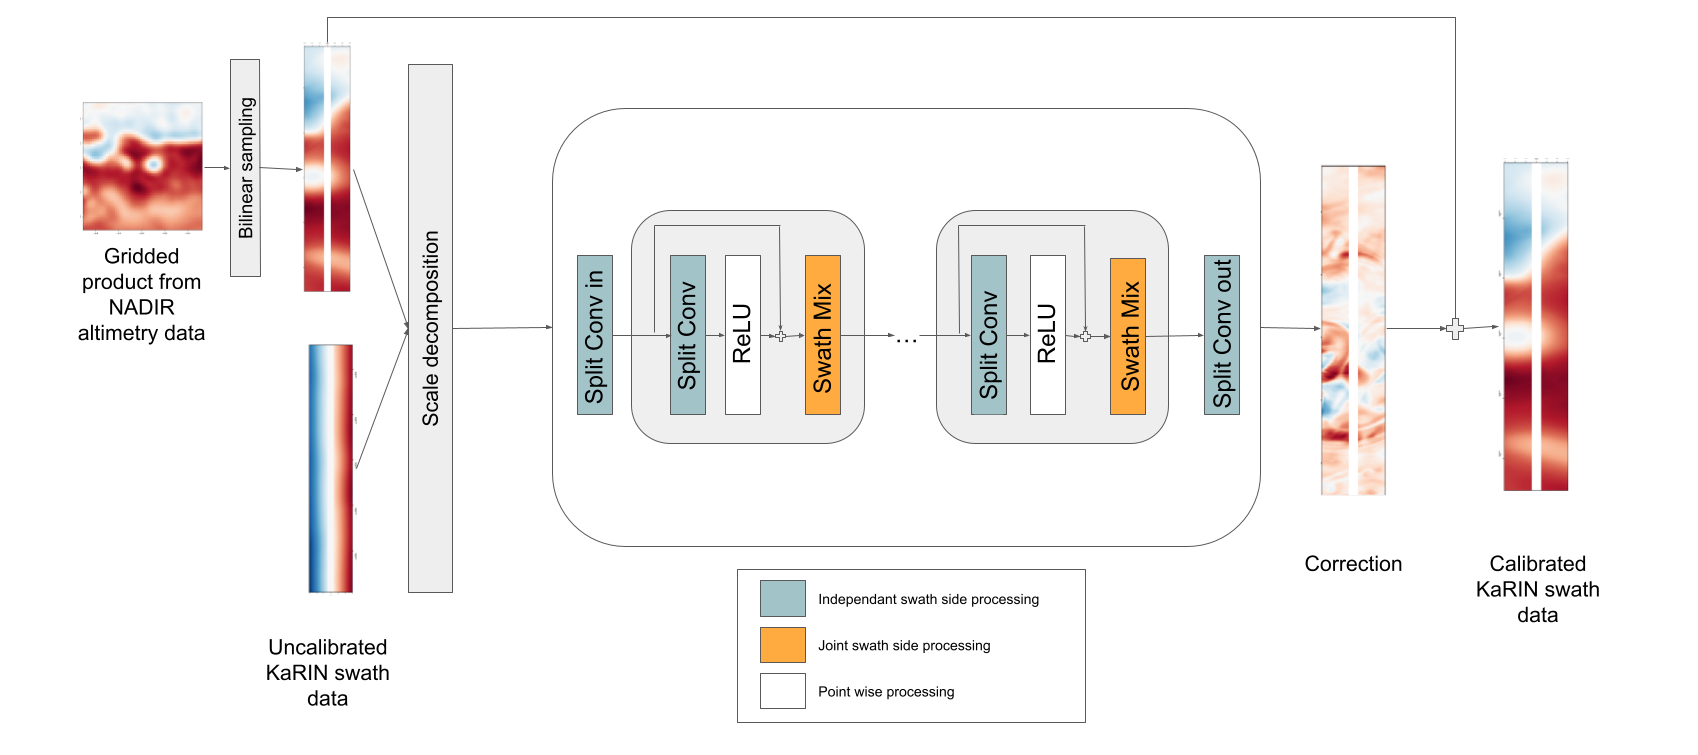
\includegraphics[width=\textwidth]{00_Calib/CalDiag2.png}
    \end{center}
    \caption{\textbf{Overview of the proposed architecture:} From left to right: The first step interpolates the nadir-based gridded product onto the swath segment. Afterwards, both the nadir-based gridded product and KaRIn observation undergo the scale-space decomposition scheme outlined in \ref{c3subsec:scale_decomp}. The scale components are stacked as channels and processed through the neural network. The blue color of the "Split Conv" indicates that each side of the swath is processed independently by the convolution layer whereas the orange coloring of the "Swath Mix" layer tells that the whole data is processed jointly (more details in \ref{c3subsec:mixing}). The final convolution computes a correction to be added to the gridded product for computing the calibrated KaRIn data}
    \label{c3fig:arch}	
\end{figure*}
The overall architecture considered is shown in figure \ref{c3fig:arch}. The scale-space decomposition block first decomposed independently the input L4 SSH products and KaRIn observations
into $N_s$-scale tensors, which we concatenate as the channel dimension.
This results into a tensor of shape $(2N_s, N_{al}, N_{ac})$ where $N_{al}$ and $N_{ac}$ are respectively the along track and across track sizes of the input swath section. The scale-space decomposition step is described in section \ref{c3subsec:scale_decomp}
A linear 2{\sc d} convolution layer follows. 
The data is then processed by a series of residual convolutional blocks composed of a convolution layer, a ReLU non-linearity \cite{Nair_Hinton_2019}, a skip connection and a swath-mixing layer as described in \ref{c3subsec:mixing}. A last linear convolution layer outputs a residual field, which we sum with the input gridded L4 SSH product to produce the calibrated KaRIn observation.
The interested reader can refer to our implementation\footnote{\url{https://github.com/CIA-Oceanix/4dvarnet-core/releases/tag/tgrs-calcnn-2023}}.



 
\subsection{Scale-space decomposition}
\label{c3subsec:scale_decomp}


We exploit a Gaussian scale-space to compute a scale-space decomposition of the fields provided as inputs to our neural architecture. For given scales $\sigma_1$ and $\sigma_2$, we extract the associated signal as the difference between filtered versions of the input signal using two Gaussian filters with standard deviation $\sigma_1$ and $\sigma_2$. We consider one-dimensional filters for the along-track direction. Formally, denoting 
 $\cal{G_{\sigma}}$ the 1-dimensional Gaussian blur operator with standard deviation $\sigma$ in the along track dimension, the considered scale-space decomposition of a signal $f$ given a sequence of increasing scales $[\sigma_1, \sigma_1, ..., \sigma_S]$ computes the following $S+1$ components: $[\mathcal{G}_{\sigma_1}(f), \mathcal{G}_{\sigma_2}(f) - \mathcal{G}_{\sigma_1}(f),...,\mathcal{G}_{\sigma_S}(f) - \mathcal{G}_{\sigma_{S-1}}(f), f - \mathcal{G}_{\sigma_S}]$
These different components are then considered as channels for the convolutionnal networks. In our experiments, we consider 20 scales in the along-track direction evenly spaced from 8km to 160km. We discuss in section \ref{c3subsec:decomp_sens} how sensitive the proposed method is to the parameterization of the decomposition.
To account for scale-dependent energy levels in the computed scale-space representation (see fig. \ref{c3fig:var_in_out}), we introduce a batch normalization layer \cite{Ioffe_Szegedy_2015}. It re-scales each component to centered and unit-variance variables.
We illustrate in Fig.\ref{c3fig:var_in_out} the impact of the batch normalization step on the relative variance of the signal of each scale of the decomposition.

One may regard the proposed scale-scale decomposition as a convolutional block. Learning such a decomposition from data would however require very large convolutional filters, which does not seem 
realistic, or a deeper architecture with pooling layers that would require very efficient optimization given the quantity of data available. 
\begin{figure}[!t]% 
    \centering
    {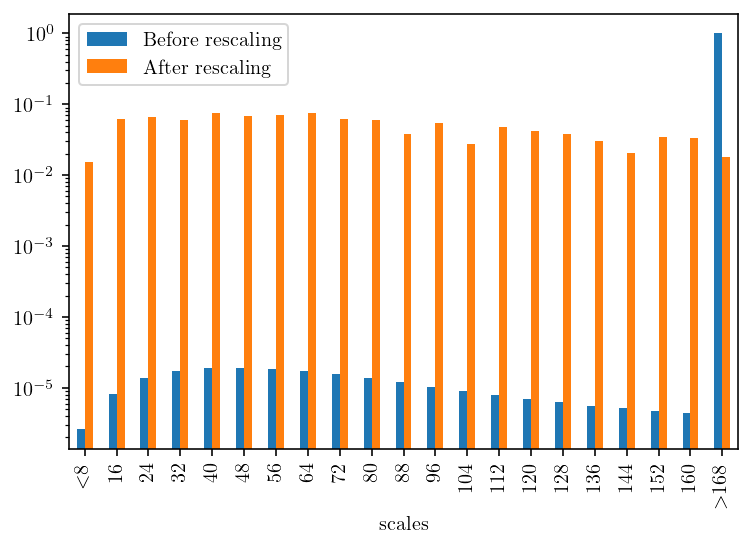
\includegraphics[width=\linewidth]{00_Calib/var_rescale_obs} }%
    \caption{\textbf{Explained variance of scale components before and after re-scaling:} Each bar indicates how much each scale component of the uncalibrated KaRIn contributes to the total variance of the signal, we can see that before re-scaling (blue) there is four orders of magnitude between largest scale and the others. The learnt re-scaling allows for scale component to be spread within a single order of magnitude (orange), which is more suited to the downstream neural architecture.}%
    \label{c3fig:var_in_out}%
\end{figure}


\subsection{Swath mixer block}
\label{c3subsec:mixing}

As observed in Figure \ref{c3fig:filtered_swath_uncal_comp}, the swath observed from the KaRIn sensor is not contiguous in the across-track dimension. The observation errors are however clearly correlated between the two sides of the swath. To exploit these correlations in our architecture, we design a swath-mixer block with two specific layers. 

To avoid convolution kernels to mix information from the two sides of the swath which could result in some unwanted side effects, each side is processed separately by each convolution layer noted "Split Conv" in Fig. \ref{c3fig:arch}. Additionally, each convolution layer input is padded so that the height and width of the input remain unchanged throughout the network.

Besides, to combine relevant features from the two sides of the swath, we introduce a layer denoted as "Swath-mix" in Fig. \ref{c3fig:arch}. It implements a convolution layer after transposing the across-track dimension as a channel dimension. This idea of a mixer layer has been used in architectures such as the MLP-Mixer \cite{mlpmixer}, in which it has been shown to help with the expressiveness of neural networks.


We analyse in section \ref{c3subsec:ablation} the contribution of the mixing layer.

\section{Experimental results}
\label{c3sec:results}

\subsection{Setup}
\noindent
The results of this section have been computed using the one year ocean simulation NATL60, over the 12°x12° domain over the Gulfstream. The model evaluation is done on forty days in the inner 10°x10° region. The training of the mapping and calibration models are done on the remaining days.
The experimental setup used is the same as in \cite{osse_data_challenge}
The base configuration for our architecture uses three convolutional blocks with 128 channels as presented in Figure \ref{c3fig:arch}.
The supervised training loss is a weighted mean of the mean square errors for the reconstruction of the SSH, its gradient and its Laplacian.
The default scale-space decomposition used is made of twenty 8 kilometers band.
The calibration model is trained for 250 epochs with a annealing triangular cyclical learning rate \cite{Smith_2017}.

\subsection{Benchmarking experiments}
\label{c3subsec:main_res}
\noindent

\begin{table}[t]
\begin{center}
\begin{tabular}{lrr}
\toprule
 & RMSE (m) & RMSE $|| \nabla_{ssh} ||$ \\
\midrule
CalCNN & 1.39e-02 & 6.46e-03 \\
UNet & 2.34e-02 & 1.07e-02 \\
4DVarNet-5nad & 2.17e-02 & 9.57e-03 \\
\bottomrule
\end{tabular}

\end{center}
\caption{Residual error of the benchmarked calibration frameworks}
\label{c3table:main}
\end{table}

We summarize our benchmarking experiments in Table \ref{c3table:main}.
We compare our approach, referred to as CalCNN, with a standard UNet \cite{Ronneberger_Fischer_Brox_2015} architecture. The latter uses as inputs the gridded altimetry product and the uncalibrated KaRIn observation stacked together as a 2{\sc d} field with 2 channels. We consider the same training configuration for this UNet model as for the CalCNN.
As baseline, we also consider the reconstruction performance for the KaRIn SSH issued from the 4DVarNet method using nadir-altimeter-only data. 
We evaluate all methods according to the following two metrics, the root mean squared error (RMSE) of the SSH field, and the RMSE of the amplitude of the gradients of the SSH field. 
Whereas the UNet fails to produce a better estimate than the nadir-only interpolation baseline, our CalCNN improves the estimation of the SSH and its gradient by over 35\% and brings the residual error below 1.4cm (Table \ref{c3table:main}).

In Figure \ref{c3fig:err_scales}, we further decompose the calibration error of the CalCNN w.r.t. the spatial scale using 1-dimensional Gaussian blurs as introduced in \ref{c3subsec:scale_decomp}. We draw a comparison with the 4DVarNet interpolation baseline and observation errors. The CalCNN reaches a lower error than both KaRIn observations and the interpolation baseline across all scales. At larger scales the error gets closer to the latter as instrument errors dominate the large-scale components of KaRIn observations. 
Interestingly, at scales lower than 10km, we still retrieve some improvement even though the observation error is quite high.
This can be explained by the fact that the high frequency errors on the KaRIn observations is easily separable from the underlying SSH signal.
Between 10-100km, our method successfully exploits the lower observation errors to improve the interpolation baseline.



\begin{figure}[!t]
    \centering
    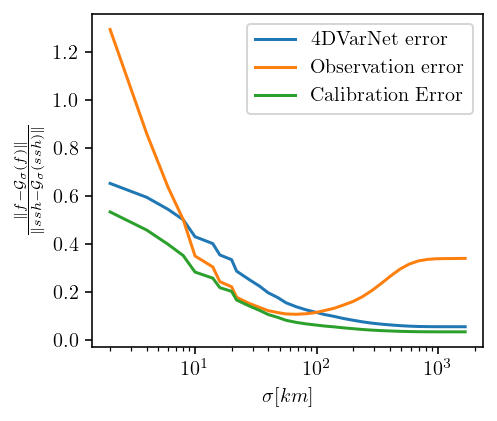
\includegraphics[width=\linewidth]
    {00_Calib/norm_cumsum_highpass_errors_1.png}%
    \caption{{\bf Observation and reconstruction error for the SSH at different spatial scales:}  The figure shows the relative error w.r.t to the SSH at different along-track scales for the inputs (Uncalibrated KaRIn in orange and nadir based interpolation in blue) and output (calibrated KaRIn in green) of our method. The x axis indicates the standard deviation of the Gaussian blur that was used to remove the high scale components of the different signals. We can see the expected trend of the interpolation error that is concentratedat fine scales. The uncalibrated KaRIn  error on the other hand is lower than the interpolation only in the 10km-100km range. We see the calibrated output of our method achieves lower error across all scales.}
    \label{c3fig:err_scales}%
\end{figure}


\subsection{Ablation Study}
\label{c3subsec:ablation}
\noindent

\begin{table}[t]
\begin{center}
\begin{tabular}{lrr}
\toprule
 & RMSE (m) & RMSE $|| \nabla_{ssh} ||$ \\
xp &  &  \\
\midrule
CalCNN & 1.39e-02 & 6.46e-03 \\
CalCNN w/o skip connection & 2.17e-02 & 9.57e-03 \\
CalCNN w/o gridded product & 1.70e-01 & 2.47e-02 \\
CalCNN w/o scale decomposition & 2.17e-02 & 9.58e-03 \\
CalCNN w/o mixing layer & 1.94e-02 & 9.60e-03 \\
\bottomrule
\end{tabular}

\end{center}
\label{c3table:ablation}
\caption{Ablation results}
\end{table}


In this section we analyse further the contribution of the different components of our neural architecture. 
In Table \ref{c3table:ablation}, we report 
the performance metrics of the considered ablation study with the following models:
a model without skip connections, one without a gridded product as input, one without the scale-space decomposition scheme (Sec. \ref{c3subsec:scale_decomp}) and one without the swath-mixer layers (Sec.\ref{c3subsec:mixing}. Overall, these four models lead to a significantly lower performance. 
The largest impact comes from the ablation of the nadir-altimetry-only gridded product which provides large-scale information about the SSH. It leads to a loss which amount to an order of magnitude in the calibration errors.
Moreover, we can see that without the skip connections or scale decomposition, we fail to improve on the L4 gridded product.
Finally, we can note that we still get a ~10\% reduction of the RMSE w.r.t the L4 product without the mixing layer, however sharing the information between each side of the swath improves this gain three fold.

% \begin{tabular}{llrrrrrrrrr}
\toprule
{}            xp &       rmse &   grad\_rmse &   spat\_res\_mean &  spat\_res\_std & \\
\midrule
     base &    0.013922 &    0.006465 &          44.991787 &     14.161194 &   \\
tgrs\_no\_decomp & 0.0216827 &   0.00958416 &  68.506 &  22.4284 \\
   no\_res &   0.021685 &    0.009566 &          68.684462 &     22.501356 &   \\
   no\_mix &   0.019368 &    0.009605 &          57.610785 &     16.674918 &   \\
   no\_xb &   0.170286 &    0.024656 &         121.735632 &     43.637274 &   \\
\bottomrule
\end{tabular}


In Table \ref{c3table:size}, we show the sensitivity to the size of the network for the same training configuration. We compare the base architecture 3x128 (3 convolution blocks with 128 channels) with a linear operator, as well as a smaller network 1x32 and a bigger one 5x512. The linear version fails to extract geophysical information from the uncalibrated information. This further points out how challenging the considered calibration task is. Interestingly, our architecture leads to a similar performance for different complexity levels. The smaller and larger architectures leads to a slight increase in the residual error but the smaller model shows a slight improvement in the gradient reconstruction and spatial resolution.
Overall, these results support the robustness of the proposed learning-based approaches and the conclusions we raise in section \ref{c3subsec:main_res} are not very sensitive to the hyper-parameters of our network architecture.
\begin{table}[t]
\begin{center}
\begin{tabular}{lrr}
\toprule
 & RMSE (m) & RMSE $|| \nabla_{ssh} ||$ \\
xp &  &  \\
\midrule
128x3 (Ref) & 1.39e-02 & 6.46e-03 \\
Linear & 2.13e-02 & 1.02e-02 \\
32x1 & 1.44e-02 & 6.22e-03 \\
512x5 & 1.49e-02 & 7.19e-03 \\
\bottomrule
\end{tabular}

\end{center}
\caption{Impact of network size}
\label{c3table:size}
\end{table}

\subsection{Gridded product sensitivity} 
\label{c3subsec:gridded_sens}
\noindent

We analyze further how the quality of nadir-altimetry-only gridded product affects the calibration performance.
In Figure \ref{c3fig:gridded_impact}, we display the improvement in the RMSE of the SSH on the swath and of the gradients of the SSH obtained by our CalCNN for the three gridded products introduced in Sec. \ref{c3subsec:interpolation}.

For all three interpolated products, the proposed calibration method improves the reconstruction of the SSH for the KaRIn swath from the joint analysis of the interpolation product and raw KaRIn observations. We report the larger improvement for DUACS product. This relates to the spectral overlap between the SSH information of the uncalibrated KaRIn and SWOT's NADIR. The associated calibration performance remains however significantly worse than that of the two 4DVarNet products, which may relate to the worse interpolation performance of DUACS product \cite{fablet_end2end_2021,osse_data_challenge}. 
When comparing the impact of the two 4DVarNet products, the results are more nuanced. The 4DVarNet-SST product leads to better metrics. The difference of RMSE is greatly reduced after calibraFKation whereas the gap in RMSE of the gradients is conserved.
This could be interpreted as the gain of RMSE we get from using the SST can be obtained from the uncalibrated KaRIn. However some of the gradients we reconstruct through the SST are not easily extracted from the observations.
Overall this shows interesting relations between the redundant information in the uncalibrated KaRIn and the interpolated products.

\begin{figure}
    \begin{center}
        % \input{gridded_impact.pgf}
        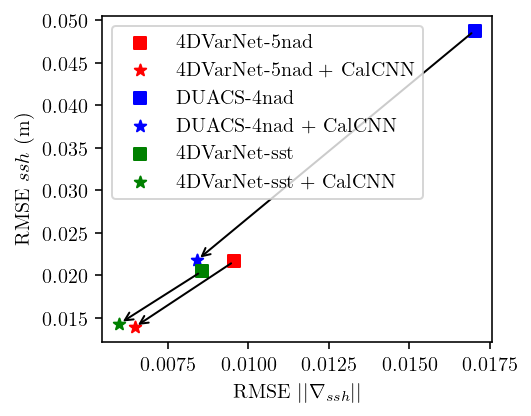
\includegraphics{00_Calib/gridded_impact.png}
    \end{center}
    \caption{{\bf Impact of the nadir-based gridded product on the CalCNN output:} The figure shows the RMSE and the RMSE of the $|| \nabla_{ssh} ||$ of the calibrated observation (stars) and their associated nadir-based gridded products (squares). The improvement brought by the CalCNN is illustrated by the arrows. This improvement can be interpreted as the relevant information extracted from the uncalibrated KaRIn by the CalCNN. Note that the biggest relative improvement concerns the DUACS gridded product (blue) which doesn't uses the SWOT's nadir altimeter.}
    \label{c3fig:gridded_impact}
\end{figure}

\subsection{Sensitivity to the scale-space decomposition}
\label{c3subsec:decomp_sens}
\noindent
In Table \ref{c3table:scale_dec}, we display the calibration metrics for different scale-space decompositions. We vary the number of scales considered and the spacing between two consecutive scales. When considering the same scale range from 8km to 160km, we retrieve the best performance with 20 scales. But, even with only 5 scales evenly separated by 32 km, the performance decreases only by 3\%.
By contrast, when considering a scale separation of 8km but varying the number of scales, we note a more significant drop of performance (about 10\% in the residual RMSE). This suggests a greater sensitivity to the span of the scale-space decomposition than to the number and spacing of the components. 
However we still achieve less than 1.6cm residual error for any of the considered variations which is still a competitive calibration outcome.

\begin{table}[!t]
\begin{center}
	\begin{tabular}{llrr}
\toprule
 &  & RMSE (m) & RMSE $|| \nabla_{ssh} ||$ \\
$N_{band}$ & $\delta_{band}$ &  &  \\
\midrule
20 & 8 & 1.39e-02 & 6.46e-03 \\
40 & 4 & 1.44e-02 & 6.64e-03 \\
10 & 16 & 1.48e-02 & 6.75e-03 \\
5 & 32 & 1.41e-02 & 6.65e-03 \\
10 & 8 & 1.56e-02 & 6.81e-03 \\
40 & 8 & 1.54e-02 & 6.88e-03 \\
\bottomrule
\end{tabular}

\end{center}
\caption{Calibration metrics in function of the scale decomposition}
\label{c3table:scale_dec}
\end{table}

\section{Conclusion}
\label{c3sec:conclusion}
\noindent
We have proposed in this chapter a neural calibration approach which combines a scale-space decomposition of KaRIn observations and a convolutional architecture. This approach proves to be robust with a 
residual error below 1.5cm which can be compared with the 2cm residual error of the expected operational approaches performance although demonstrated globally using a different ocean simulation \cite{Dibarboure_Ubelmann_Flamant_Briol_Peral_Bracher_Vergara_Faugere_Soulat_Picot_2022}. While we can reach a satisfactory calibration performance using the operational nadir altimetry mapping product, our experiments highlight the potential benefit of ongoing effort on neural SSH interpolation schemes to further improve the retrieval of finer-scale features from KaRIn observations.
This naturally advocates for future work exploring jointly calibration and mapping problems for nadir and wide-swath altimeters, possibly combining our deep learning approach and variational mapping formulations introduced in \cite{Febvre_Fablet_Sommer_Ubelmann_2022}.
The generalization to real signals of our calibration operator trained on simulated data is obviously a key challenge to be investigated.

\addcontentsline{toc}{section}{Bibliography}

% \begin{thebibliography}{biblio}
% \bibliographystyle{IEEEbib}
% \bibliography{biblio}
% \end{thebibliography}
\begin{thebibliography}{10}

\bibitem{Peral_Esteban-Fernandez_2018}
E.~Peral et~al.,
\newblock ``Swot mission performance and error budget,''
\newblock in {\em IGARSS 2018 - 2018 IEEE International Geoscience and Remote
  Sensing Symposium}, Jul 2018, p. 8625–8628.

\bibitem{ubelmann_swot_nodate}
C.~Ubelmann, et~al.,
\newblock ``{SWOT} {Simulator} documentation,'' .

\bibitem{Dibarboure_Ubelmann_Flamant_Briol_Peral_Bracher_Vergara_Faugere_Soulat_Picot_2022}
G.~Dibarboure, et~al.,
\newblock ``Data-driven calibration algorithm and pre-launch performance
  simulations for the swot mission,''
\newblock {\em Remote Sensing}, vol. 14, no. 2323, pp. 6070, Jan 2022.

\bibitem{Witkin_1984}
A.~Witkin,
\newblock ``Scale-space filtering: A new approach to multi-scale description,''
\newblock in {\em ICASSP ’84. IEEE International Conference on Acoustics,
  Speech, and Signal Processing}, Mar 1984, vol.~9, p. 150–153.

\bibitem{taburet_duacs_2019}
G.~Taburet, et~al.,
\newblock ``{DUACS} {DT2018}: 25 years of reprocessed sea level altimetry
  products,''
\newblock {\em Ocean Science}, vol. 15, no. 5, pp. 1207--1224, 2019.

\bibitem{glorys_rea_2021}
J-M.~Lellouche, et~al.,
\newblock ``The copernicus global 1/12° oceanic and sea ice glorys12
  reanalysis,''
\newblock {\em Frontiers in Earth Science}, vol. 9, pp. 585, 2021.

\bibitem{beauchamp_intercomparison_2020}
M.~Beauchamp, et~al.,
\newblock ``Intercomparison of {Data}-{Driven} and {Learning}-{Based}
  {Interpolations} of {Along}-{Track} {Nadir} and {Wide}-{Swath} {SWOT}
  {Altimetry} {Observations},''
\newblock {\em Remote Sensing}, vol. 12, no. 22, 2020.

\bibitem{fablet_end2end_2021}
R.~Fablet, et~al.,
\newblock ``{END}-{TO}-{END} {PHYSICS}-{INFORMED} {REPRESENTATION} {LEARNING}
  {FOR} {SATELLITE} {OCEAN} {REMOTE} {SENSING} {DATA}: {APPLICATIONS} {TO}
  {SATELLITE} {ALTIMETRY} {AND} {SEA} {SURFACE} {CURRENTS},''
\newblock {\em ISPRS Annals of the Photogrammetry, Remote Sensing and Spatial
  Information Sciences}, vol. V-3-2021, pp. 295--302, 2021.

\bibitem{osse_data_challenge}
M.~Ballarota, et~al.,
\newblock ``ocean-data-challenges/2020a\_ssh\_mapping\_natl60: Material for ssh
  mapping data challenge,'' Sep 2020.

\bibitem{lindeberg1996edge}
T.~Lindeberg,
\newblock ``Edge detection and ridge detection with automatic scale
  selection,''
\newblock in {\em IEEE CVPR}. IEEE, 1996, pp. 465--470.

\bibitem{Lindeberg_2015}
T.~Lindeberg,
\newblock ``Image matching using generalized scale-space interest points,''
\newblock {\em Journal of Mathematical Imaging and Vision}, vol. 52, no. 1, pp.
  3–36, May 2015.

\bibitem{Pintea_Tomen_Goes_Loog_van_Gemert_2021}
S.~L. Pintea, et~al.,
\newblock ``Resolution learning in deep convolutional networks using
  scale-space theory,''
\newblock {\em IEEE Transactions on Image Processing}, vol. 30, pp.
  8342–8353, Jan 2021.

\bibitem{Worrall_Welling_2019}
D.~Worrall et~al.,
\newblock ``Deep scale-spaces: Equivariance over scale,''
\newblock in {\em Advances in Neural Information Processing Systems}. 2019,
  vol.~32, Curran Associates, Inc.

\bibitem{lecun98}
Y.~Lecun, et~al.,
\newblock ``Gradient-based learning applied to document recognition,''
\newblock {\em Proceedings of the IEEE}, vol. 86, no. 11, pp. 2278–2324, Nov
  1998.

\bibitem{resnet2016}
K.~He, et~al.,
\newblock ``Deep residual learning for image recognition,''
\newblock 2016, p. 770–778.

\bibitem{liu_image_2018}
G.~Liu, et~al.,
\newblock ``Image inpainting for irregular holes using partial convolutions,''
\newblock in {\em Proceedings of the {European} {Conference} on {Computer}
  {Vision} ({ECCV})}, 2018, pp. 85--100.

\bibitem{yolo2016}
J.~Redmon, et~al.,
\newblock ``You only look once: Unified, real-time object detection,''
\newblock 2016, p. 779–788.

\bibitem{colin2021}
A.~Colin, et~al.,
\newblock ``Segmentation of sentinel-1 sar images over the ocean, preliminary
  methods and assessments,''
\newblock in {\em 2021 IEEE International Geoscience and Remote Sensing
  Symposium IGARSS}, Jul 2021, p. 4067–4070.

\bibitem{colin_2022}
A.~Colin, et~al.,
\newblock ``Semantic segmentation of metoceanic processes using sar
  observations and deep learning,''
\newblock {\em Remote Sensing}, vol. 14, no. 44, pp. 851, Jan 2022.

\bibitem{fablet_joint_2021}
R.~Fablet, et~al.,
\newblock ``Joint {Interpolation} and {Representation} {Learning} for
  {Irregularly} {Sampled} {Satellite}-{Derived} {Geophysical} {Fields},''
\newblock {\em Frontiers in Applied Mathematics and Statistics}, vol. 7, 2021.

\bibitem{li_convolutional_2022}
X.~Li, et~al.,
\newblock ``A {Convolutional} {Neural} {Network}-{Based} {Relative}
  {Radiometric} {Calibration} {Method},''
\newblock {\em IEEE Transactions on Geoscience and Remote Sensing}, vol. 60,
  pp. 1--11, 2022,
\newblock Conference Name: IEEE Transactions on Geoscience and Remote Sensing.

\bibitem{Ronneberger_Fischer_Brox_2015}
O.~Ronneberger, et~al.,
\newblock ``U-net: Convolutional networks for biomedical image segmentation,''
\newblock , no. arXiv:1505.04597, May 2015,
\newblock arXiv:1505.04597 [cs].

\bibitem{ajayi_spatial_2020}
A.~Ajayi, et~al.,
\newblock ``Spatial and {Temporal} {Variability} of the {North} {Atlantic}
  {Eddy} {Field} {From} {Two} {Kilometric}-{Resolution} {Ocean} {Models},''
\newblock {\em Journal of Geophysical Research: Oceans}, 125, 5.
  e2019JC015827, 2020.

\bibitem{carrassi_data_2018}
A.~Carrassi, et~al.,
\newblock ``Data assimilation in the geosciences: {An} overview of methods,
  issues, and perspectives,''
\newblock {\em Wiley Interdisciplinary Reviews: Climate Change}, vol. 9, no. 5,
  pp. e535, Sept. 2018,
\newblock Publisher: Wiley.

\bibitem{Beauchamp_Febvre_Georgenthum_Fablet_2022}
M.~Beauchamp, et~al.,
\newblock ``4dvarnet-ssh: end-to-end learning of variational interpolation
  schemes for nadir and wide-swath satellite altimetry,''
\newblock {\em Geoscientific Model Development Discussions}, vol. 2022, pp.
  1–37, 2022.

\bibitem{Fablet_Febvre_Chapron_2022}
R.~Fablet, et~al.,
\newblock ``Multimodal 4dvarnets for the reconstruction of sea surface dynamics
  from sst-ssh synergies,''
\newblock , arXiv:2207.01372, Jul 2022.

\bibitem{Nair_Hinton_2019}
V.~Nair et~al.,
\newblock ``Rectified linear units improve restricted boltzmann machines,''
\newblock Jul 2019.

\bibitem{Ioffe_Szegedy_2015}
S.~Ioffe et~al.,
\newblock ``Batch normalization: Accelerating deep network training by reducing
  internal covariate shift,''
\newblock in {\em Proceedings of the 32nd International Conference on Machine
  Learning}. Jun 2015, p. 448–456, PMLR.

\bibitem{mlpmixer}
I.~O. Tolstikhin, et~al.,
\newblock ``Mlp-mixer: An all-mlp architecture for vision,''
\newblock in {\em Advances in Neural Information Processing Systems}. 2021,
  vol.~34, p. 24261–24272, Curran Associates, Inc.

\bibitem{Smith_2017}
L.~N. Smith,
\newblock ``Cyclical learning rates for training neural networks,''
\newblock in {\em 2017 IEEE Winter Conference on Applications of Computer
  Vision (WACV)}, Mar 2017, p. 464–472.

\bibitem{Febvre_Fablet_Sommer_Ubelmann_2022}
Q.~Febvre, et~al.,
\newblock ``Joint calibration and mapping of satellite altimetry data using
  trainable variational models,''
\newblock in {\em IEEE ICASSP 2022 - 2022}, May 2022, p. 1536–1540.

\end{thebibliography}


\end{bibunit}
%\begin{IEEEbiographynophoto}{Quentin Febvre}
%Quentin Febvre is a 2nd year PhD student at IMT Atlantique Brest
%\end{IEEEbiographynophoto}

% \begin{IEEEbiography}[{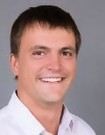
\includegraphics[width=1in,height=1.25in,clip,keepaspectratio]{photo_qfebvre.jpg}}]{Quentin Febvre}
% recived the graduate degree from the École Supérieure d'électricité, France and  Master of Science degree in Computer Science from Tsinghua University, China in 2015. He then worked as a data scientist for an international advertising company in 2016 before joining Theodo Group in Paris where he worked on web development, data engineering and computer vision applications using data driven approaches. In 2020, he started as a PhD student in the Mathematical and Electrical engineering department at IMT Atlantique Bretagne-Pays de la Loire. His research focuses on the benefits deep learning approaches can bring to ocean observation systems, and more specifically on altimetry data analysis.
% %\begin{IEEEbiographynophoto}{Ronan Fablet}

% \end{IEEEbiography}

% \end{document}




\clearemptydoublepage
%%%%%%%%%%%%%%%%%%%%%%%%%%%%%%%%%%%%%%%%%%%%%%%%%%%%%%%%%%%%%%%%%%%%%%%%%%%%
% AGUJournalTemplate.tex: this template file is for articles formatted with LaTeX
%
% This file includes commands and instructions
% given in the order necessary to produce a final output that will
% satisfy AGU requirements, including customized APA reference formatting.
%
% You may copy this file and give it your
% article name, and enter your text.
%
% guidelines and troubleshooting are here: 

%% To submit your paper:
% \documentclass[draft]{agujournal2019}
% \usepackage{url} %this package should fix any errors with URLs in refs.
% \usepackage{lineno}
% \usepackage{booktabs}
% \usepackage{graphicx}
% \usepackage{subcaption}
% \usepackage{float}

% % \usepackage[inline]{trackchanges} %for better track changes. finalnew option will compile document with changes incorporated.
% \usepackage{soul}
% \linenumbers
%%%%%%%
% As of 2018 we recommend use of the TrackChanges package to mark revisions.
% The trackchanges package adds five new LaTeX commands:
%
%  \note[editor]{The note}
%  \annote[editor]{Text to annotate}{The note}
%  \add[editor]{Text to add}
%  \remove[editor]{Text to remove}
%  \change[editor]{Text to remove}{Text to add}
%
% complete documentation is here: http://trackchanges.sourceforge.net/
%%%%%%%

% \draftfalse

%% Enter journal name below.
%% Choose from this list of Journals:
%
% JGR: Atmospheres
% JGR: Biogeosciences
% JGR: Earth Surface
% JGR: Oceans
% JGR: Planets
% JGR: Solid Earth
% JGR: Space Physics
% Global Biogeochemical Cycles
% Geophysical Research Letters
% Paleoceanography and Paleoclimatology
% Radio Science
% Reviews of Geophysics
% Tectonics
% Space Weather
% Water Resources Research
% Geochemistry, Geophysics, Geosystems
% Journal of Advances in Modeling Earth Systems (JAMES)
% Earth's Future
% Earth and Space Science
% Geohealth
%
% ie, \journalname{Water Resources Research}

% \journalname{Journal of Advances in Modeling Earth Systems (JAMES)}


% \begin{document}

%%%%%%%%%%%%%%%%%%%%%%%%%%%%%%%%%%%%%%%%%%%%%%%
%  TITLE
%
% (A title should be specific, informative, and brief. Use
% abbreviations only if they are defined in the abstract. Titles that
% start with general keywords then specific terms are optimized in
% searches)
%
%%%%%%%%%%%%%%%%%%%%%%%%%%%%%%%%%%%%%%%%%%%%%%%

% Example: \title{This is a test title}

% \title{Training neural mapping schemes for satellite altimetry with ocean model data}


% \authors{Q. Febvre\affil{1}, J. Le Sommer\affil{2}, C. Ubelmann\affil{3}, R. Fablet\affil{1}}

% \affiliation{1}{IMT Atlantique, Lab-STICC, Brest, France}
% \affiliation{2}{Université Grenoble Alpes, CNRS, IRD, Grenoble, France}
% \affiliation{3}{Datlas, Grenoble, France}

% \correspondingauthor{Quentin Febvre}{quentin.febvre@imt-atlantique.fr}



% \begin{keypoints}
% \item We propose a simulation-based training approach for the neural mapping of real satellite-derived observations.
% \item Simulation-trained neural schemes significantly outperform the operational mapping of real altimetry data for a Gulf Stream case-study.
% \item More realistic simulation datasets improve the performance of the trained neural mapping both quantitatively and qualitatively. 

% \end{keypoints}

\begin{bibunit}[IEEEtran.bst]

\clearemptydoublepage
\chapter{Training neural mapping schemes for satellite altimetry with ocean model data}

\begin{abstract}
  The absence of reference data, which defines the expected model outputs, poses a challenge when training machine learning models with ocean observations. Here, we put forward the idea that leveraging both simulated observations and ocean quantities for learning purposes provides a powerful method to develop real-world applications.
  For example, we focus here on the problem of satellite altimetry interpolation which consist in reconstructing the dynamic field of sea surface height (SSH) from satellite observations that have a high rate of missing data and irregular sampling. Data-driven models have been successfully demonstrated for this task in supervised settings using an observation simulated system experiment (OSSE), i.e. with a simulated SSH field as learning target and pseudo-observations as inputs.
  However the learning paradigm used in those demonstrations can not be trivially transferred to real altimetry observations by lack of knowledge of the true SSH field.
  We ask here if and under what condition the knowledge extracted from synthetic data transfers to real observations. We study the impact of the ocean run resolution, observation data reanalysis and of explicit tide modeling on training an interpolator over the Gulfstream region. We find that the different datasets reliably offers better performance than the current operational product DUACS when evaluated on real altimetry data. Additionally, a more realistic ocean simulation through higher resolution or model reanalysis has been shown to be significant for achieving better reconstruction performance on our test case. Our best model improves the longitudinal scale resolved from 151 kilometers for DUACS to 98 kilometers and improves the root mean squared error (RMSE) by 23\%.
  We believe that this work opens interesting perspectives for developing synergies between ocean modeling and operational product development by leveraging learning based approaches.

\end{abstract}

\section*{Plain Language Summary}

% https://www.agu.org/Share-and-Advocate/Share/Community/Plain-language-summary
In order for an artificial intelligence to learn, one need to describe a task using data and an evaluation procedure. For example, to train a model to recognize trees, one need pictures of trees and the labels of the type of tree in the pictures to evaluate and train the model.
For some problems we have access to a lot of data but cannot easily train a model because we can't easily tell how good it's performing. This happens in ocean science where a lot of instruments gather observation data but it's not always easy to compute what the model should be trained for.
Here we look at a specific task which is to construct images related to the ocean surface currents from what satellites can see. The satellite data we're using can be seen as an image of the ocean surface with a lot of missing data (~95\% of missing pixels for a given day), and we would like to train an artificial intelligence to find the values of the missing pixels.
As described before, when our model fills the gaps a certain way, we cannot easily say how good is the reconstruction because we don't know the full image. It is therefore challenging to train such an artificial intelligence using only the satellite data.
However, scientists know a lot about the ocean, how the currents behave and they're able to simulate fake oceans in big computers. For these fake oceans, we do have access to the gap-free image, so we can train A.I. models by first hiding some pixels and checking if the model fill the gaps with the correct values.
In this paper we explore if A.I.s trained on fake oceans are useful for the real ocean and study what is the best fake ocean for training an A.I.
We show that today's fake oceans work well for training an A.I. on this specific task and that the best way to obtain a great A.I. is to use a fake ocean that has been simulated with a higher resolution!


\section{Introduction}


% ML pour traitement de données satellite, bcp d'applications recentes 

% en particulier tache de gap-filling et cartoigraphie 

% un bon exemple altimétrie, methodes expertes et methodes methodes basées données. 

%--- [difficulté : suprenante, pas vraiment assez de données pour entrainer algo complexe (millions partame) [en fait non]]

% algo basé donnée : modele parametrique (calibration faible nombre de params : MIOST, DYNMOST), algo issue du DL (grnd nombre de param, NN expressif, peu d'hypothese)

% algo DL, besoin de bcp de données, en prqtique, peuvent entrainée sur données modeles. ex papier de SEATTLE. (emergence : modele numerique pour ca.) 

% question comment se fait le tranfert, sous quelle condition un lodele est-il bon poru entrainer algo pour tache donées reel. 

% Dans cet article, on demontre que modele peut marcher, cas particuler altimétrie, influence de la donnée d'entrée 

% le plan de l'artle, c'est ca 



  Satellite altimeters have brought a great leap forward in the observation of sea surface height on a global scale since the 80's. They have greatly contributed to the monitoring and understanding of key processes such as the rise of the mean ocean level due to rising temperature and the role of mesoscale dynamics.
  
  The retrieval of mesoscale-to-submesoscale sea surface dynamics for horizontal scales smaller than 150 km however remains a challenge for operational systems based on optimal interpolation \cite{taburetDUACSDT2018252019} and data assimilation \cite{jean-michelCopernicusGlobal122021} schemes. This has motivated a wealth of research to develop novel mapping schemes \cite{ballarottaDynamicMappingAlongTrack2020,ubelmannReconstructingOceanSurface2021,guillouMappingAltimetryForthcoming2021}.

  In this context, data-driven and learning-based approaches \cite{alveraazcarateReconstructionIncompleteOceanographic2005,barthDINCAEMultivariateConvolutional2022,lguensatAnalogDataAssimilation2017,fabletENDTOENDPHYSICSINFORMEDREPRESENTATION2021,martinSynthesizingSeaSurface2023} appear as appealing alternatives to make the most of the available simulation and observation datasets. Especially, Observing System Simulation Experiments (OSSE) have stressed the potential of the supervised learning of neural schemes for the mapping of satellite-derived altimetry data \cite{fabletENDTOENDPHYSICSINFORMEDREPRESENTATION2021,beauchamp4DVarNetSSHEndtoendLearning2023}. 
  
  Their applicability to real datasets has yet to be assessed and recent studies have rather explored unsupervised learning strategies from real gappy multi-year altimetry datasets \cite{martinSynthesizingSeaSurface2023}. Despite promising results, these schemes do not reach the relative improvement of the operational processing suggested by OSSE-based studies.
  
Here, we go beyond the exploitation of OSSE as benchmarking-only testbeds. We explore their use for the training of neural mapping schemes which we apply to real altimetry dataset. Through numerical experiments on a Gulf Stream case-study for 2003-2005 4-nadir altimeter constellation, our key contributions are as follows:  

    \begin{itemize}
    \item{We demonstrate the relevance of the supervised OSSE-based learning of neural mapping schemes for the space-time interpolation of real nadir altimetry data;}
    \item{We benchmark the proposed approach with state-of-the-art operational products as well as neural schemes trained from real altimetry datasets;}    
    \item{We benchmark neural schemes trained with the proposed OSSE-based strategy using different simulation datasets and we assess the impact of the characteristics of these datasets on the mapping performance.}
%    Demonstrate numerically that today's numerical simulations of the ocean are a valuable resource for training machine learning models to be applied on real data, with added benefit of more realistic synthetic data}
    \end{itemize}
To ensure the reproducibility of our results, our code is made available through an open source license along with the considered datasets and the trained models.

    
The content of this paper is organized in the following manner. Section \ref{sec:background} offers background information on related work, Section \ref{sec:method} presents our method, Section \ref{sec:results} reports our numerical experiments, and Section \ref{sec:discussion} elaborates on our main contributions.



\section{Background}
\label{sec:background}
\subsection{Satellite altimetry gridded products}
\label{ssec:interpolation}
The mapping of altimetry data to produce gridded products is a necessary step to observe surface dynamics since geostrophic currents depend on the SSH gradients which cannot be directly computed from one dimensional altimetry data. We can distinguish three categories of approaches to produce such maps. 

Data assimilation products that use large ocean models such as the GLORYS12 reanalysis \cite{jean-michelCopernicusGlobal122021}. These products leverage the full expressiveness of state of the art ocean models and aims at generating trajectories close to observed quantities through data assimilation methods such as Kalman filters and four dimensional variational data assimilation (4DVAR)\cite{carrassiDataAssimilationGeosciences2018}. In the case of the GLORYS12 reanalysis, alitmetry data was assimilated as well as ocean salinity, surface temperature and sea-ice concentration observations.

Then, observation products that are made with little dynamical assumptions such as optimal-interpolation-based product DUACS \cite{taburetDUACSDT2018252019} or methods that involve simplified quasi-geostrophic dynamics to guide the interpolation scheme. \cite{guillouMappingAltimetryForthcoming2021},\cite{ballarottaDynamicMappingAlongTrack2020}

Finally in recent years, data-driven interpolation schemes including neural network based approaches recently gained momentum \cite{alveraazcarateReconstructionIncompleteOceanographic2005,fabletENDTOENDPHYSICSINFORMEDREPRESENTATION2021,ubelmannReconstructingOceanSurface2021}.



\subsection{Ocean Modeling and OSSE}
\label{ssec:oceanmodeling}
Efforts in modeling and simulating ocean physics have been essentials for better understanding the processes involved in the earth system and being able to project future behaviours \cite{bernardImpactPartialSteps2006,ajayiSpatialTemporalVariability2020}. 
High resolution simulations used in Observing System Simulation Experiments (OSSE) also provide a great test-bed for developing and evaluating new ways observing the ocean.
Access to the numerical model outputs enables the computation of interpretable metrics directly on the quantities of interest. This can be challenging when working with observation data which need to go through a series of processing steps to estimate before being interpretable.
For example, in the case of the recently launched SWOT mission, a novel instrument has been deployed and the calibration methods were developed and evaluated using ocean and instrument simulations \cite{dibarboureDataDrivenCalibrationAlgorithm2022}.
Similarly, the development of new methods for interpolating altimetry tracks and SWOT data such as the BFN-QG and 4DVarNet were also first demonstrated in OSSE setups \cite{guillouMappingAltimetryForthcoming2021,fabletENDTOENDPHYSICSINFORMEDREPRESENTATION2021}. 



\subsection{Tackling the lack of annotated data}
\label{ssec:transferlearning}
In OSSE setups, learning based mapping schemes can be trained on reconstructing the model outputs considered as the ground truth during evaluation. However such training procedures cannot be trivially transferred  when transitioning to Observing System Experiments (OSE) by lack of knowledge of the ocean state.
Applied machine learning practitioners often face the challenge of limited annotated data when training supervised learning schemes since creating large annotated datasets for a given task can be expensive or infeasible.
Prior research efforts have tackled this issue by either leveraging existing related annotated datasets such as the ImageNet\cite{dengImageNetLargescaleHierarchical2009} dataset to train general purpose computer vision models \cite{heDeepResidualLearning2016}. Another approach involves generating synthetic data to facilitate the creation of annotated items. \cite{gomezgonzalezVIPVortexImage2017,dosovitskiyFlowNetLearningOptical2015}.
We propose that ocean model output can be considered as a large synthetic annotated dataset for a variety of task. Recent work have used simulation data to train super-resolution model of the SSH \cite{buongiornonardelliSuperResolvingOceanDynamics2022} later evaluated on observation data. Our work aims to further investigate the potential of such training schemes. 



\subsection{Physics-aware deep-learning}
\label{ssec:deeplearning}
In the last decades, machine learning advances combined with the rise in computational resources and amount of data have shown the power of extracting knowledge from data in a variety of domains ranging from computer vision to language processing. 
However one fundamental limitation of learning from data is the bad generalization performance outside the the training distribution. This is of critical importance for physical systems, where training a learning-based model on past data will seldom perform well when the system evolves and reaches dynamics absent from the training data. We can see evidence of this shortcoming in the instability challenges faced by neural closures for climate models \cite{brenowitzInterpretingStabilizingMachineLearning2020}. 
On the flip side, physical laws grant practically unlimited capacity for generalization in any given scenario, yet they fall short of fully capitalizing on the knowledge embedded in the accessible data.

There have been a variety of approaches trying to harness the best of both world. Some injects trainable components in classical integration scheme of physical model such as \cite{yinAugmentingPhysicalModels2021b}. Others leverage physical prior within their learning setups which can been used in the training objective \cite{raissiPhysicsinformedNeuralNetworks2019,greydanusHamiltonianNeuralNetworks2019}, as well as in the architecture \cite{li2020fourier,Wang2020TF}. 

However most of these works have focused on relatively simple physical models and it remains challenging to combine current state of the art ocean models with such methods. Obstacles include the complexity and cost of running the physical model, the differences in programming tools and infrastructure used in each domain, as well the difficulty of computing the gradients of an integration step of the ocean model.

In this paper we would like to push for the idea that a great way to benefit from the advances made by the ocean modeling community is to use high-resolution runs of ocean models as training data to learn deep neural model for ocean reanalysis. 





\section{Method}
\label{sec:method}


\subsection{Overview}
\label{ssec:overview}

In this section, we describe the proposed method for assessing the potential of OSSE-trained neural mapping schemes for the mapping real altimetry tracks. We describe the architecture considered in our study, as well as the different datasets used for training the mapping algorithm. We then go into more detail on how we designed our OSSE setup for training and the method used for evaluating our trained model on real altimetry.  

\begin{figure}[ht]
    \centering
    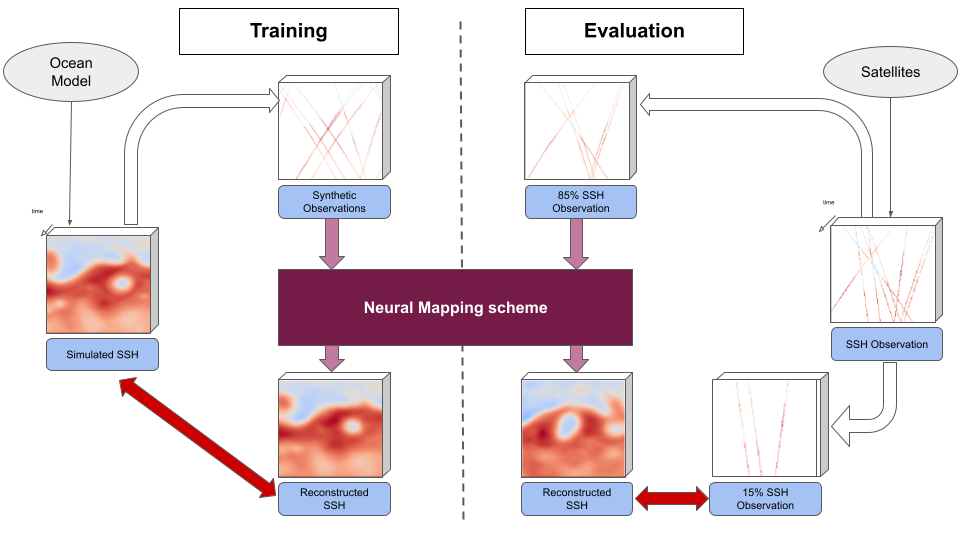
\includegraphics[width=\textwidth]{00_Simulearning/figures/schema_method.png}
    \caption{Overview of the experimental setup. On the left side we display the OSSE training principle based on an ocean simulation which will be used for 1) generating synthetic observation and 2) computing the training objective of the neural mapping scheme. On the right side we show the evaluation principle of splitting the available satellite observations to evaluate the method on data that were not used for the inference.}
    \label{fig:method}
\end{figure}


\subsection{Neural mapping scheme}
\label{ssec:4dvarnet}

We consider the 4DVarNet model for our study. It's a variational data assimilation method where the prior cost formulated using a physically-aware convolutional neural network, and the minimization procedure is done using a recurrent neural network as introduced by \cite{andrychowiczLearningLearnGradient}.
The overall architecture and components are the same as the one described in previous publications \cite{fabletENDTOENDPHYSICSINFORMEDREPRESENTATION2021}. Some changes in the implementation details have been made that were found to empirically improve the performance and reduce the training time. We refer the reader to the code for more details.
This architecture reaches state of the art performance when evaluated in OSSE setup which makes it a good candidate for assessing the generalization to real data


\subsection{SSH Data}
\label{ssec:data}

\begin{table}[h]

\begin{tabular}{ll||cccc}
\toprule
{} & {}& Resolution & Reanalysis & Tide & DAC  \\
\midrule
NATL60 &\cite{ajayiSpatialTemporalVariability2020}               &      1/60 $^\circ$ &               No &            No &                   No  \\
eNATL60-t &\cite{brodeauOceannextENATL60Material2020}         &      1/60 $^\circ$ &               No &           Yes &                  Yes  \\
eNATL60-0 &\cite{brodeauOceannextENATL60Material2020}         &      1/60 $^\circ$ &               No &            No &                  Yes  \\
GLORYS12-r &\cite{jean-michelCopernicusGlobal122021} &      1/12 $^\circ$ &              Yes &            No &                   No  \\
GLORYS12-f &\cite{jean-michelCopernicusGlobal122021}   &      1/12 $^\circ$ &               No &            No &                   No  \\
ORCA025& \cite{bernardImpactPartialSteps2006}             &       1/4 $^\circ$ &               No &            No &                   No  \\
\bottomrule
\end{tabular}
\caption{Summary table of the different synthetic SSH fields used for training}
\label{tab:data}
\end{table}



Digital ocean models are intricate software programs that incorporate numerous configuration parameters. In order to better isolate influence factors, we considered runs of the NEMO\cite{gurvanNEMOOceanEngine2022} ocean model with different configurations. We selected six distinct datasets to examine the influence of three factors on the dynamical structures manifested in the simulations.

In order to evaluate the impact of the grid resolution used for the simulation, we consider the runs NATL60, ORCA025 and the free run of GLORYS12-f  which are respectively run at  1/60°, 1/12°, 1/4°. We know that finer grids allow for more processes to be simulated. We expect dynamics to therefore be closer to the real ocean in higher resolution simulations and the associated trained deep learning model to perform better.
Another way to nudge ocean simulations to more realistic dynamics is by assimilating observation data. To evaluate this aspect we compare the GLORYS12-r reanalysis and its associated the free run GLORYS12-f. Measurements of temperature, sea level, sea ice concentration and salinity have been assimilated during the reanalysis. This comparison will also give indication on the impact of using true observation during the training.
Finally the recent eNATL60 twin simulations  eNATL60-t and eNATL60-0 enable us to evaluate impact of explicit modeling of tide motions.
The characteristics of the different simulation are summarized in Table \ref{tab:data}

\subsection{OSSE training setup}
\label{ssec:training}
The training setup is illustrated on the left part of the Figure \ref{fig:method}.
In order to fairly evaluate the datasets' quality as a training resource, we strive to standardize as many training aspects as possible.
All simulations are regridded to the same resolution (1/20°) and daily averages are used as training target. We generate noise-free pseudo-observations by sampling values of the daily averages corresponding to realistic orbits of a 5 altimeter-constellation. All models are trained using one-year synthetic dataset in a domain around the Gulfstream from (66°W, 32°N) to (54°W, 44°N) in which the same two months are kept for validation. The hyper-parameters of the model and training procedure such as the number of epoch, learning rate scheduler are the same for all the experiments. The models are trained on reconstructing the SSH fields and the amplitude of the gradients as well as a regularization cost on the prior model.

\subsection{OSE evaluation setup}
\label{ssec:eval}
The training setup is illustrated on the right part of the Figure \ref{fig:method}.
The evaluation is done using altimetry data from the constellation of 6 satellites from 2017 (SARAL/Altika, Jason 2, Jason 3, Sentinel 3A, Haiyang-2A and Cryosat-2 ). Five satellites are used as inputs for the mapping and one (Cryosat-2) is kept out for computing the metrics. The metrics are computed in the track geometry on which the gridded product is interpolated on the altimetry tracks. The evaluation domain spans from (65°W, 33°N) to (55°W, 43°N)  and the periods goes from January 1$^{st}$ to December 31$^{st}$ 2017. This setup is standardized in a data-challenge \footnote{https://github.com/ocean-data-challenges/2021a\_SSH\_mapping\_OSE} where various methods have been compared on two metrics. Given $\eta_{c2}$ and $\hat{\eta}$ the measured SSH and the reconstructed SSH respectively; $\mu_{ssh}$ is a score based on the normalized root mean squared (nRMSE) error  computed as $1 - \frac{RMS(\hat{\eta} - \eta_{c2})}{RMS(\eta_{c2})}$ and $\lambda_x$ is the wavelength at which the PSD score  $1 - \frac{PSD(\hat{\eta} - \eta_{c2})}{PSD(\eta_{c2})}$ crosses the $0.5$ threshold, which characterize the scales resolved by the reconstruction (the error below that wavelength is make for more that half of the signal). We reuse these metrics for our study and also consider in Table \ref{tab:res} the root mean square error (RMSE) as well as the nRMSE score of the sea level anomaly $\mu_{sla}$ obtained by subtracting the mean dynamic topography to the SSH. We also assess the performance degradation resulting from the transition from simulated to real data by quantifying the improvement relative to DUACS in scales resolved within OSSE and OSE scenarios.

\section{Results}
\label{sec:results}

\subsection{Benchmarking w.r.t the state of the art}
\label{ssec:benchmarks}

We report in Table \ref{tab:bench} the performance metrics of state of the art approaches ranging from operational observation products, deep learning based mapping schemes trained on observation data as well as methods using explicit integration of a dynamical model.
We compare those methods with the 4DVarNet trained on the eNATL60-0 dataset during this study. 
The OSSE-trained 4DVarNet outperform all other methods on the two metrics considered (22\% improvement in RMSE w.r.t. the DUACS product and 33\% improvement in resolved scales)
We add in this table the GLORYS12 reanalysis metrics which illustrates the challenge of combining large ocean general circulation model and observation data for producing operational observation products.


The last column of the table compares the improvement of $\lambda_x$ with regard to DUACS of the different methods with a simulated setups using the NATL60 simulation in which some of this methods have been evaluated \footnote{https://github.com/ocean-data-challenges/2020a\_SSH\_mapping\_NATL60}. We clearly see how the supervised setting using the full model output as a training target is greatly beneficial to the 4DVarNet in the simulated which achieve an improvement of 47\% twice greater than the second best at 22\%. We can however note that this improvement by 15 point for the OSSE-trained mapping shceme when other methods are significantly more stable. We can deduce that the finer structures that are well reconstructed in the OSSE setup are not as beneficial in the OSE setup. We can attribute this to multiple hypothesis, either they may not be representative of the true ocean, or the real altimetry tracks may limit the ability to reconstruct and/or evaluate them.  



\begin{table}[h]
%\centering
\hspace{-10mm}\begin{tabular}{l||llll|rrrc}
\toprule
 & SSH  & Deep  & Calibrated on  & Physical  & rmse & $\mu_{ssh}$  & $\lambda_x$ & $1 - \frac{\lambda_x}{\lambda_{ref}}$ \\
 &  Only &  Learning &  data from &  Model &  (cm) &  () &  (km) & (\% ose, osse) \\
\midrule
(a) \textbf{4DVarNet} &  Yes & Yes & Simulation  & -- & \textbf{5.9}  & \textbf{0.91}  & \textbf{100} & \textbf{33}, \textbf{47} \\
(b) MUSTI & No &  Yes & Satellite  & -- & 6.3  & 0.90  & 112 & 26, 22 \\
(c) ConvLstm-SST & No &  Yes & Satellite  & -- & 6.7  & 0.90  & 108 & 28, -- \\
(d) ConvLstm &  Yes &  Yes & Satellite  & -- & 7.2  & 0.89  & 113 & 25, -- \\
(e) DYMOST&  Yes & No & Satellite  & QG & 6.7  & 0.90  & 131 & 13, 11 \\
(f) MIOST &  Yes & No & Satellite  & -- & 6.8  & 0.90  & 135 & 11, 10 \\
(g) BFN-QG &  Yes & No & Satellite  & QG & 7.6  & 0.89  & 122 & 19, 21 \\
(h) DUACS &  Yes & No & Satellite  & -- & 7.7  & 0.88  & 151 &  ~0,  0 \\
(i) GLORYS12 & No & No & Satellite  & NEMO & 15.1  & 0.77  & 241 & -60, -- \\
\bottomrule
\end{tabular}
\caption{ Benchmark of different methods on the SSH reconstruction of Gulfstream domain: (a) 4dVarNet trained on eNATL60-0 (b) \cite{archambaultMultimodalUnsupervisedSpatioTemporal2023}, (c and d) \cite{martinSynthesizingSeaSurface2023}, (e) \cite{ballarottaDynamicMappingAlongTrack2020}, (f) \cite{ubelmannReconstructingOceanSurface2021}, (g) \cite{guillouMappingAltimetryForthcoming2021}, (h) \cite{taburetDUACSDT2018252019}, (i) \cite{jean-michelCopernicusGlobal122021}. The columns indicate in order: whether ancillary data other than altimetry tracks were used for the mapping (for example sea surface temperature observation products); if the method uses deep learning architectures; the data used to calibrate (or train) the method parameters; the numerical model of the ocean used for the mapping if any (QG stands for quasi-geostrophic); $\mu$ and $\lambda_x$ are the metrics as described in \ref{ssec:eval}}
\label{tab:bench}
\end{table}



\begin{figure}[H]
\begin{minipage}{.80\linewidth}
\begin{subfigure}[t]{.9\linewidth}
\small
\begin{center}
\setlength{\tabcolsep}{1pt}

\begin{tabular}[t]{c@{}cccccc}

\hspace{0cm} ORCA025 & 
 GLORYS12-f & 
 GLORYS12-r & 
 NATL60 & 
 eNATL60-t & 
 eNATL60-0 & \\

%\vspace{-2mm}
%%%%% ORCA025 %%%%%%%%

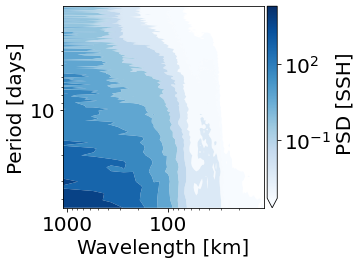
\includegraphics[trim={0 19mm 35mm 5mm},clip, width=2.3cm,height=2cm]{00_Simulearning/figures/plots2/orca025_train_psd_spacetime.png} &
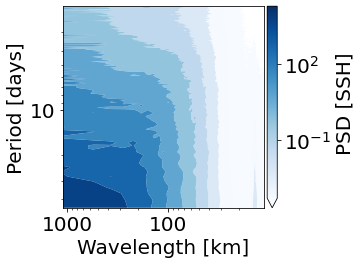
\includegraphics[trim={19mm 19mm 35mm 5mm},clip, width=2cm,height=2cm]{00_Simulearning/figures/plots2/glorys12-f_train_psd_spacetime.png} &
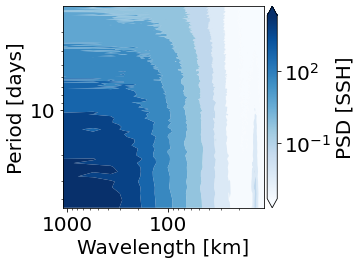
\includegraphics[trim={19mm 19mm 35mm 5mm},clip, width=2cm,height=2cm]{00_Simulearning/figures/plots2/glorys12-r_train_psd_spacetime.png} &
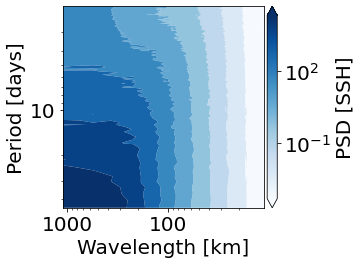
\includegraphics[trim={19mm 19mm 35mm 5mm},clip, width=2cm,height=2cm]{00_Simulearning/figures/plots2/natl60_train_psd_spacetime.png} &
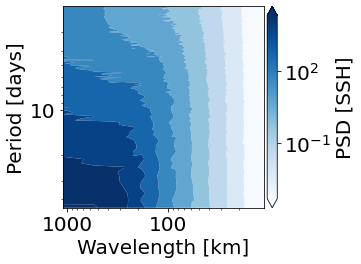
\includegraphics[trim={19mm 19mm 35mm 5mm},clip, width=2cm,height=2cm]{00_Simulearning/figures/plots2/enatl60-t_train_psd_spacetime.png} &
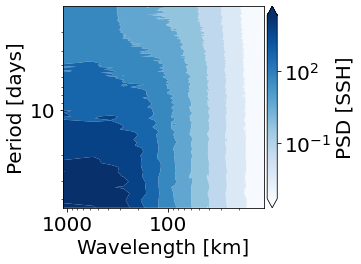
\includegraphics[trim={19mm 19mm 35mm 5mm},clip, width=2cm,height=2cm]{00_Simulearning/figures/plots2/enatl60-0_train_psd_spacetime.png} &
 \\
%\vspace{3mm}
%%%%% GLORYS12-f %%%%%%%%

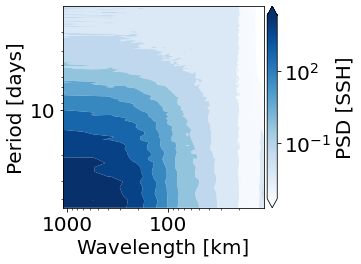
\includegraphics[trim={0mm 0 35mm 5mm},clip, width=2.3cm,height=2.3cm]{00_Simulearning/figures/plots2/orca025_rec_psd_spacetime.png} &
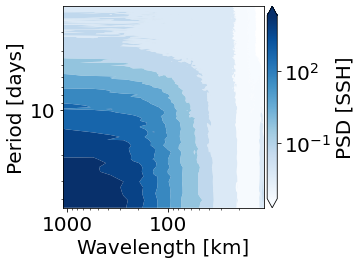
\includegraphics[trim={19mm 0 35mm 5mm},clip, width=2cm,height=2.3cm]{00_Simulearning/figures/plots2/glorys12-f_rec_psd_spacetime.png} &
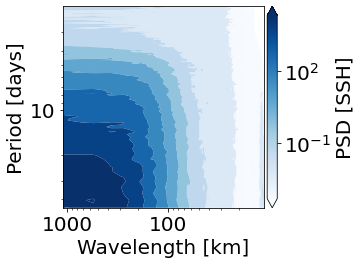
\includegraphics[trim={19mm 0 35mm 5mm},clip, width=2cm,height=2.3cm]{00_Simulearning/figures/plots2/glorys12-r_rec_psd_spacetime.png}&
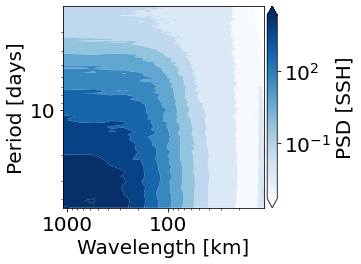
\includegraphics[trim={19mm 0 35mm 5mm},clip, width=2cm,height=2.3cm]{00_Simulearning/figures/plots2/natl60_rec_psd_spacetime.png}&
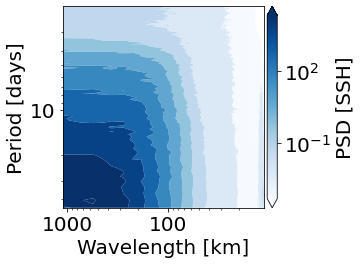
\includegraphics[trim={19mm 0 35mm 5mm},clip, width=2cm,height=2.3cm]{00_Simulearning/figures/plots2/enatl60-t_rec_psd_spacetime.png} &
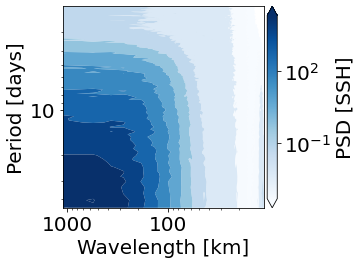
\includegraphics[trim={19mm 0 35mm 5mm},clip, width=2cm,height=2.3cm]{00_Simulearning/figures/plots2/enatl60-0_rec_psd_spacetime.png}  &
\\

\end{tabular}
% \caption{Row I - Isotrophic PSD. Row 2 - Isotrophic PSD Score}

\end{center}

\end{subfigure}
\end{minipage}
\hspace{1.5cm}\begin{minipage}{0.01\linewidth}
\vspace{-.5cm}

\begin{subfigure}[t]{.9\linewidth}
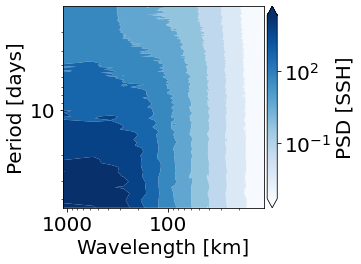
\includegraphics[trim={9.4cm 0 0 0},clip, width=0.88cm,height=2.52cm]{00_Simulearning/figures/plots2/enatl60-0_train_psd_spacetime.png}
\end{subfigure}
\end{minipage}
\caption{
Space-time spectral densities of the training datasets (first row) and their associated reconstructions (second row). We see how finer resolution and reanalysis increase the energy levels at all scales in the while the reconstructions' PSDs are more alike but with still visible differences especially in the temporal axis} \vspace{-5mm}
\label{fig:spacetime_psd}
\end{figure}




\begin{figure}[H]
\small
\begin{center}
\setlength{\tabcolsep}{1pt}
\begin{tabular}{ccccc}
 &&
&\hspace{-30mm} 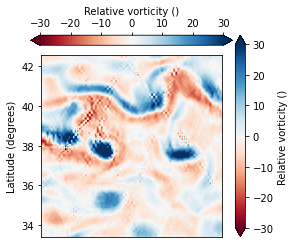
\includegraphics[trim={8mm 7cm 22mm 0},clip,width=3.0cm,height=0.7cm]{00_Simulearning/figures/plots/horizontal_cbar_vort.png} &\\
\hspace{0mm} &&
\hspace{-30mm} Training  
\hspace{3mm}  & 
 & 
\hspace{-30mm} Reconstruction \\

%\vspace{-2mm}
%%%%% ORCA025 %%%%%%%%

\hspace{-10mm}  1)&
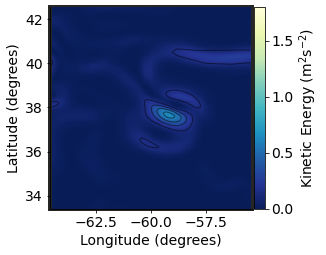
\includegraphics[trim={0 16mm 26mm 5mm},clip, width=3.3cm,height=2.9cm]{00_Simulearning/figures/plots2/orca025_train_ke.png} &
 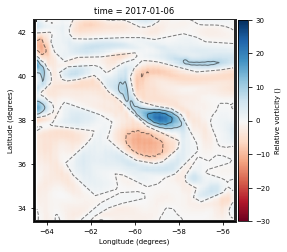
\includegraphics[trim={13mm 13mm 22mm 6mm},clip, width=2.9cm,height=2.9cm]{00_Simulearning/figures/plots/orca025_train_vort_r.png} &
 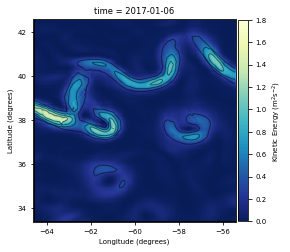
\includegraphics[trim={13mm 13mm 22mm 6mm},clip, width=2.9cm,height=2.9cm]{00_Simulearning/figures/plots/orca025_rec_ke.png} &
 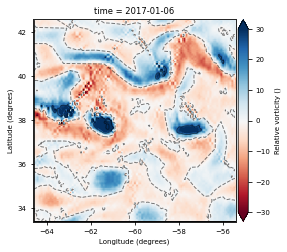
\includegraphics[trim={13mm 13mm 22mm 6mm},clip,width=2.9cm,height=2.9cm]{00_Simulearning/figures/plots/orca025_rec_vort_r.png} \\
%\vspace{3mm}
%%%%% GLORYS12-f %%%%%%%%
\hspace{-10mm} 2) &
 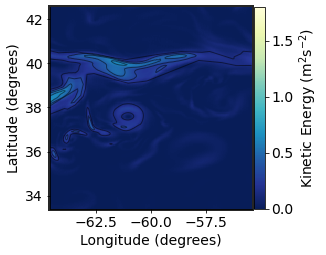
\includegraphics[trim={0 16mm 26mm 5mm},clip, width=3.3cm,height=2.9cm]{00_Simulearning/figures/plots2/glorys12-f_train_ke.png} &
 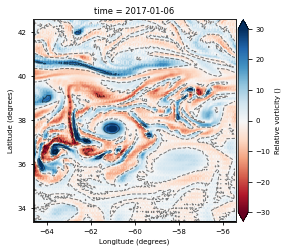
\includegraphics[trim={13mm 13mm 22mm 6mm},clip, width=2.9cm,height=2.9cm]{00_Simulearning/figures/plots/glorys12-f_train_vort_r.png} &
 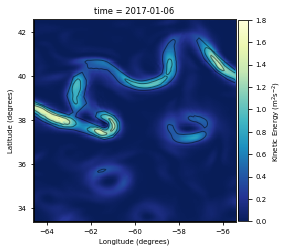
\includegraphics[trim={13mm 13mm 22mm 6mm},clip, width=2.9cm,height=2.9cm]{00_Simulearning/figures/plots/glorys12-f_rec_ke.png} &
 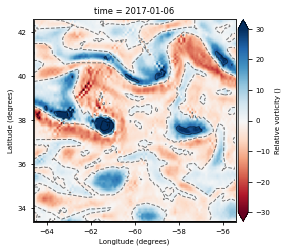
\includegraphics[trim={13mm 13mm 22mm 6mm},clip,width=2.9cm,height=2.9cm]{00_Simulearning/figures/plots/glorys12-f_rec_vort_r.png} \\
%\vspace{3mm}
%%%%% GLORYS12-f %%%%%%%%
\hspace{-10mm} 3) &
 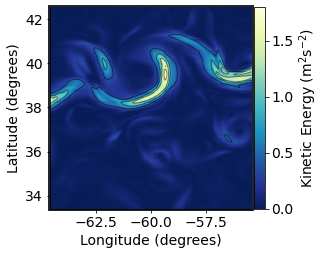
\includegraphics[trim={0 16mm 26mm 5mm},clip, width=3.3cm,height=2.9cm]{00_Simulearning/figures/plots2/glorys12-r_train_ke.png} &
 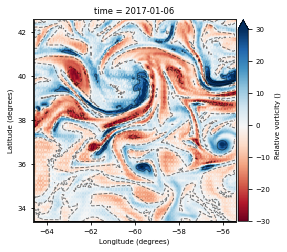
\includegraphics[trim={13mm 13mm 22mm 6mm},clip, width=2.9cm,height=2.9cm]{00_Simulearning/figures/plots/glorys12-r_train_vort_r.png} &
 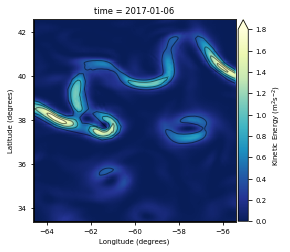
\includegraphics[trim={13mm 13mm 22mm 6mm},clip, width=2.9cm,height=2.9cm]{00_Simulearning/figures/plots/glorys12-r_rec_ke.png} &
 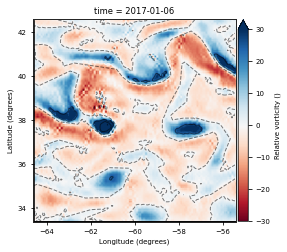
\includegraphics[trim={13mm 13mm 22mm 6mm},clip,width=2.9cm,height=2.9cm]{00_Simulearning/figures/plots/glorys12-r_rec_vort_r.png} \\
%%%%% NATL60 %%%%%%%%
\hspace{-10mm} 4) &
 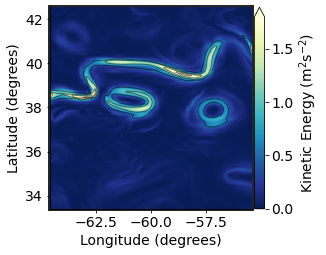
\includegraphics[trim={0 16mm 26mm 5mm},clip, width=3.3cm,height=2.9cm]{00_Simulearning/figures/plots2/natl60_train_ke.png} &
 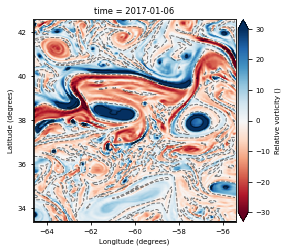
\includegraphics[trim={13mm 13mm 22mm 6mm},clip, width=2.9cm,height=2.9cm]{00_Simulearning/figures/plots/natl60_train_vort_r.png} &
 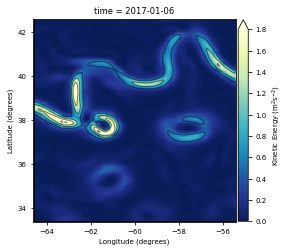
\includegraphics[trim={13mm 13mm 22mm 6mm},clip, width=2.9cm,height=2.9cm]{00_Simulearning/figures/plots/natl60_rec_ke.png} &
 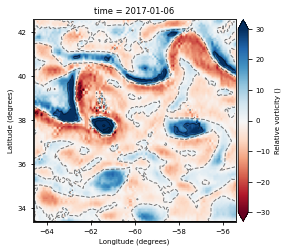
\includegraphics[trim={13mm 13mm 22mm 6mm},clip,width=2.9cm,height=2.9cm]{00_Simulearning/figures/plots/natl60_rec_vort_r.png} \\
%\vspace{3mm}
%%%%% eNATL60-t %%%%%%%%
\hspace{-10mm} 5) &
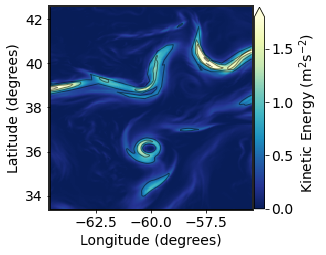
\includegraphics[trim={0 16mm 26mm 5mm},clip, width=3.3cm,height=2.9cm]{00_Simulearning/figures/plots2/enatl60-t_train_ke.png} &
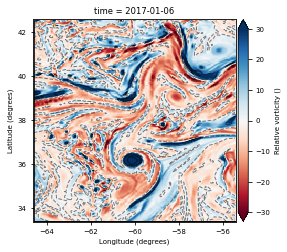
\includegraphics[trim={13mm 13mm 22mm 6mm},clip, width=2.9cm,height=2.9cm]{00_Simulearning/figures/plots/enatl60-t_train_vort_r.png} &
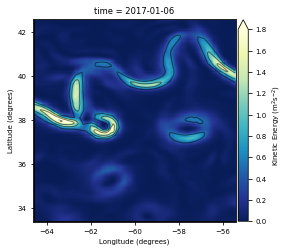
\includegraphics[trim={13mm 13mm 22mm 6mm},clip, width=2.9cm,height=2.9cm]{00_Simulearning/figures/plots/enatl60-t_rec_ke.png} &
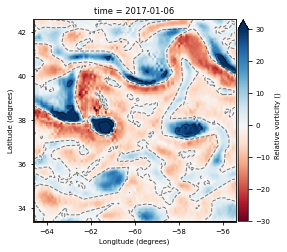
\includegraphics[trim={13mm 13mm 22mm 6mm},clip,width=2.9cm,height=2.9cm]{00_Simulearning/figures/plots/enatl60-t_rec_vort_r.png} \\
%\vspace{3mm}
%%%%% eNATL60-0 %%%%%%%%
% \hspace{-10mm} 6) &
%  \includegraphics[trim={0 0 19mm 5mm},clip, width=3.3cm,height=3.1cm]{00_Simulearning/figures/plots2/enatl60-0_train_ke.png} &
%  \includegraphics[trim={13mm 0 22mm 5mm},clip, width=2.9cm,height=3.1cm]{00_Simulearning/figures/plots2/enatl60-0_train_vort_r.png} &
%  \includegraphics[trim={13mm 0 22mm 5mm},clip, width=2.9cm,height=3.1cm]{00_Simulearning/figures/plots2/enatl60-0_rec_ke.png} &
%  \includegraphics[trim={13mm 0 22mm 5mm},clip,width=2.9cm,height=3.1cm]{00_Simulearning/figures/plots2/enatl60-0_rec_vort_r.png} \\
 \hspace{-10mm} 6) &
 \includegraphics[trim={0 0 25mm 5mm},clip, width=3.3cm,height=3.1cm]{00_Simulearning/figures/plots2/enatl60-0_train_ke.png} &
 \includegraphics[trim={18mm 0 26mm 5mm},clip, width=2.9cm,height=3.1cm]{00_Simulearning/figures/plots2/enatl60-0_train_vort_r.png} &
 \includegraphics[trim={18mm 0 26mm 5mm},clip, width=2.9cm,height=3.1cm]{00_Simulearning/figures/plots2/enatl60-0_rec_ke.png} &
 \includegraphics[trim={18mm 0 26mm 5mm},clip,width=2.9cm,height=3.1cm]{00_Simulearning/figures/plots2/enatl60-0_rec_vort_r.png} \\
 \hspace{-15mm} &(a) & (b) & (c) & (d) \\
 &&
&\hspace{-30mm} \includegraphics[trim={8mm 0 22mm 7cm},clip,width=2.5cm,height=0.7cm]{00_Simulearning/figures/plots/horizontal_cbar_ke_bottom.png} &\\
% \vspace{-2mm}

\end{tabular}
\vspace{-3mm}
% \caption{Row I - Isotrophic PSD. Row 2 - Isotrophic PSD Score}
\caption{
Kinetic energy ((a) and (c) and relative vorticity ((b) and (d)) of the training dataset ((a) and (b)) and the associated 4DVarNet reconstructions ((c) and (d)) at the 6$^th$ of January of their respective year.
Each row shows the experiment using: 1) ORCA025, 2) GLORYS12-f, 3) GLORYS12-r, 4) NATL60, 5) eNATL60-t, 6) eNATL60-0}
\vspace{-5mm}
\label{fig:maps}
\end{center}
\end{figure}



\begin{table}[H]
\centering
\begin{tabular}{l||rrrrc}
\toprule
Training Data & RMSE  & $\mu_{ssh}$  & $\mu_{sla}$ & $\lambda_x$ & $1 - \frac{\lambda_x}{\lambda_{ref}}$ \\
 &  (cm) &  () &  () &  (km) & (\% ose, osse) \\
\midrule
NATL60 & \textbf{5.9}  & \textbf{0.91}  & \textbf{0.80}  & \textbf{98} & (\textbf{35}, --)\\
eNATL60-t & \textbf{5.9}  & \textbf{0.91}  & \textbf{0.80}  & 100 & (33, \textbf{48})\\
eNATL60-0 & \textbf{5.9}  & \textbf{0.91}  & \textbf{0.80}  & 100 & (33, 47)\\
GLORYS12-r & 6.3  & 0.90  & 0.78  & 106  & (30, 28)\\
GLORYS12-f & 6.7  & 0.90  & 0.77  & 119 & (21, 23)\\
ORCA025 & 7.1  & 0.89  & 0.76  & 126 & (17, 17)\\
\bottomrule
\end{tabular}

\caption{Performance comparison of 4dVarNet mapping schemes trained on different simulated datasets. The first column show the source of the training dataset as described in Table \ref{tab:data}. The subsequent columns indicate the reconstruction metrics described in Section \ref{ssec:eval}. Note that the NATL60 could not be evaluated on the OSSE setup since the evaluation data were used for validation during the training stage.}
\label{tab:res}
\end{table}

\subsection{Eddy-permitting vs eddy-resolving simulations}
\label{ssec:resolution}


\begin{figure}[H]
\small
\setlength{\tabcolsep}{1pt}
\begin{tabular}{ccc}

\hspace{3mm} Training PSD & 
\hspace{3mm} Reconstruction PSD & 
\hspace{3mm} PSD Score  \\

%\vspace{-2mm}
%%%%% ORCA025 %%%%%%%%

\includegraphics[width=0.31\textwidth]{00_Simulearning/figures/plots2/isotrop_psd_res_train.png} &
\includegraphics[width=0.31\textwidth]{00_Simulearning/figures/plots2/isotrop_psd_res_rec.png} &
\includegraphics[width=0.31\textwidth]{00_Simulearning/figures/plots2/res_1d_psd_score.png}


\end{tabular}
\vspace{-3mm}
% \caption{Row I - Isotrophic PSD. Row 2 - Isotrophic PSD Score}
\caption{
Impact of the resolution on the PSDs. We display the PSD of the training dataset (left plot), reconstructed SSH field (center plot) as well as the associated PSD score (right plot)}\vspace{-5mm}
\label{fig:respsd}
\end{figure}


We analyse here in more detail the impact of ocean run resolution in the training data and reconstructed fields. Looking at quantitative metrics in Table \ref{tab:res} we see the expected trend that using a higher resolution grid in the ocean run simulation enables a better outcome with a 22\% improvement in scales resolved and 17\% improvement in RMSE between the experiments with the coarsest (ORCA025) and finest (NATL60) resolution.
Qualitative differences can also been seen in the relative vorticity fields in Figure \ref{fig:maps} where residual artifacts due to the altimetry tracks can be seen (60°W, 39°N) for the two lower resolution training and are greatly diminished when looking at the NATL60 resolution. 
However we see that the reconstructed vorticity and kinetic energy of the ORCA025 experiment are quite similar to the one from the NATL60 experiment despite the ORCA025 training data clearly containing fewer fine scale structures an weaker gradients. The trained model is able to reconstruct fields outside the training distribution when prompted with observations different from the training data. 

This is also visible in the spectral densities shown in Figure \ref{fig:respsd} where we see that the gap in energy distribution of the training data has been significantly reduced in the reconstructions, however the PSD score plot on the right shows that even if the energy levels are close in the reconstructions, training with finer resolution produces a more faithful reconstruction at all scales.
Finally when looking at the space-time PSD in Figure \ref{fig:spacetime_psd}, we can note that even though the spatial spectra have been greatly homogenized, the temporal PSD still contains significant gaps of an order of magnitude for periods greater than 10 days and wavelength greater than 200km.

\subsection{Impact of reanalysis datasets}
\label{ssec:reanalysis}
\begin{figure}[h]

\small

\setlength{\tabcolsep}{1pt}
\begin{tabular}{ccc}

\hspace{3mm} Training PSD & 
\hspace{3mm} Reconstruction PSD & 
\hspace{3mm} PSD Score  \\

%\vspace{-2mm}
%%%%% ORCA025 %%%%%%%%

\includegraphics[width=0.31\textwidth]{00_Simulearning/figures/plots2/isotrop_psd_rea_train.png} &
\includegraphics[width=0.31\textwidth]{00_Simulearning/figures/plots2/isotrop_psd_rea_rec.png} &
\includegraphics[width=0.31\textwidth]{00_Simulearning/figures/plots2/rea_1d_psd_score.png}


\end{tabular}
\vspace{-3mm}
% \caption{Row I - Isotrophic PSD. Row 2 - Isotrophic PSD Score}
\caption{
Impact of model reanalysis on the PSDs. We display the PSD of the training dataset (left plot), reconstructed SSH field (center plot) as well as the associated PSD score (right plot)}\vspace{-5mm}
\label{fig:reapsd}

\end{figure}

Looking in more specifically at the effect of ocean reanalysis between the two experiments GLORYS12-f and GLORYS12-r. We can first note the impact of observation data assimilation in Figure \ref{fig:spacetime_psd} where we see how the power spectrum of the reanalysis is significantly raised compared to the free run and is similar the one of the finer resolution simulation. Visually on the maps in Figure \ref{fig:maps}, we can also clearly see stronger gradients in the kinetic energy.

We can observe a similar behavion as in section \ref{ssec:resolution} in Figure \ref{fig:reapsd} with the gap of in spectral density being diminished between the training and reconstruction data, and the PSD score indicating a lower energy of the error at all scales for the reanalyzed experiment.

Quantitatively in Table \ref{tab:data} we see an improvement of 11\% in both the RMSE and the scale resolved, and one singular fact is that training on a reanalysis increase the relative gain w.r.t. DUACS significantly more on real data (+9\%) than on simulated data (+5\%) as we can right most column. This can be explained thanks to the fact the training data integrates information from real world observations which reduces the generalization problem to real altimetry mapping.

\subsection{Impact of tide-resolving numerical simulations}
\label{ssec:tide}
\begin{figure}[H]
\small
\begin{center}
\setlength{\tabcolsep}{1pt}
\begin{tabular}{ccc}

\hspace{3mm} Training PSD & 
\hspace{3mm} Reconstruction PSD & 
\hspace{3mm} PSD Score  \\

%\vspace{-2mm}
%%%%% Tide psd %%%%%%%%

\includegraphics[width=0.31\textwidth]{00_Simulearning/figures/plots2/isotrop_psd_tide_train.png} &
\includegraphics[width=0.31\textwidth]{00_Simulearning/figures/plots2/isotrop_psd_tide_rec.png} &
\includegraphics[width=0.31\textwidth]{00_Simulearning/figures/plots2/tide_1d_psd_score.png}


\end{tabular}
\vspace{-3mm}
% \caption{Row I - Isotrophic PSD. Row 2 - Isotrophic PSD Score}
\caption{
Impact of explicit tide modelling on the PSDs. We display the PSD of the training dataset after the prepocessing (left plot), the reconstructed SSH field (center plot) as well as the associated PSD score (right plot)}\vspace{-5mm}
\label{fig:tidepsd}
\end{center}
\end{figure}

We compare here the effect of explicit tide modeling in the training simulation. For this we use the twin eNATL60 simulation runs eNATL60-t and eNATL60-0.  Contrary to other runs, those simulation contains barometric and wind forcing, we therefore remove the Dynamic Atmospheric Correction from the SSH fields. Additionally since the barotropic tides signal are removed from real altimetry tracks prior to interpolation, we also remove this signal from the training data by subtracting the spatial mean over the training domain for each hourly snapshot before calculating the daily averages.  

After those processing steps, we see that the two training datasets contain very similar spectral profiles as shown in Figures \ref{fig:spacetime_psd} and \ref{fig:tidepsd}. 
We also find that training on those two dataset produce little differences in the reconstructions both quantitatively \ref{tab:bench} and qualitatively (Fig. \ref{fig:maps}) and both experiments' results are comparable to the NATL60 experiment.
 
We identify two hypothesis linked to the lack of impact of resolving tides during the simulation:
\begin{itemize}
    \item The preprocessing applied on the training field remove the main tide signals. We therefore effectively measure the impact of tide modeling on other ocean processes that may be less significant.
    \item The evaluation procedure applied on altimetry tracks on which the barotropic tide has been filtered may not be interpretable enough to measure the reconstruction of residual tide signals. New instruments like the KaRIN deployed in the SWOT mission may provide new ways to better quantify those effects.   
\end{itemize}

These findings provide motivation for carefully considering the purpose of the learning-based model when making decisions about the training data. Indeed In our case, explicitly modeling tide processes that are removed from the observations in the evaluation setup added overhead in the computational cost of running the simulation as well as in the preprocessing of the training data. Additionally given the considered evaluation data and metrics, we were not able to quantify any significant differences between the two trained mapping schemes.

On the other hand training on a simulation with tide could also be a way to reduce the processing steps on the observation data by being able to interpolate observation containing the tide signals.

\section{Discussion}
\label{sec:discussion}
This study has been greatly facilitated by the standardized tasks and evaluation setups proposed in data-challenges \footnote{https://ocean-data-challenges.github.io/}. The specification of problems by domain experts through datasets and relevant evaluation metrics have been instrumental in constituting the comprehensive benchmark combining methods from different teams and institution around the world. Additionally, it also constitutes a strong basis for multi-disciplinary collaboration between the ocean and machine learning research communities.

Moreover, the results presented in this study introduce a direct relation between ocean simulations and the performance of altimetry products. This opens new ways for ocean physicist, modelers and operational oceanographers to collaborate. In order to assess the range of these new synergies, it would be interesting to explore if the approach proposed here of training altimetry mapping schemes using simulation data would generalize to other tasks such as forecast or sensor calibration and to other quantities like surface temperature, currents, salinity or biochemical tracers.

If the approach turns out generic enough, one could envision training large foundation deep learning models capturing the inner structure of high resolution ocean simulations which could then be used in many downstream applications. This could be the way to capitalize on all the advancement in ocean modeling without having to run OGCM numerical simulation for each downstream products.    

As a final point we would like to highlight the cost consideration when running numerical simulation intended for training learning based schemes. Indeed given that the eNATL60 run took 2700x CPU hours and 350x memory compared to the ORCA025 run for a smaller domain, a trade-off arises between generating multiple "cheap" trajectories versus generating  a single more realistic trajectory. 

\section{Conclusion}
\label{sec:conclusion}
We've seen in this study that training machine learning models on simulations offers reliably good performance on real altimetry data mapping and outperforms current state of the art approaches. Even the coarsest simulation considered ORCA025 provides competitive results with current operational methods. We have shown that using a more realistic SSH fields using reanalysis or higher resolution simumlations increases the performances of the trained model. This is an exciting result that shows the potential for training operational products from ocean simulations and how advances in ocean modeling in operational oceanography can be beneficial. The results shown here are limited to the interpolation problem on a regional domain but the robustness of the performance shown are encouraging for further developing these results using a bigger domain.


\addcontentsline{toc}{section}{Bibliography}
\putbib[./00_Simulearning/biblio]
\end{bibunit}
% \bibliography{biblio}

% \section*{Open Research Section}
% The authors provide the training data, source code, reconstructed maps and trained model for each experiments of the manuscript through the following link https://doi.org/10.5281/zenodo.8064114.



% \acknowledgments
% This work was supported by ANR Projects Melody and OceaniX and CNES. It benefited from HPC and GPU resources from GENCI-IDRIS (Grant 2020-101030) and Ifremer.


% \bibliography{biblio}



% \end{document}







\clearemptydoublepage
\documentclass{article}



% if you need to pass options to natbib, use, e.g.:
%     \PassOptionsToPackage{numbers, compress}{natbib}
% before loading neurips_data_2023

% ready for submission
% \usepackage{neurips_data_2023}
\usepackage[preprint]{neurips_data_2023}

% to compile a preprint version, add the [preprint] option, e.g.:
%     \usepackage[preprint]{neurips_data_2023}
% This will indicate that the work is currently under review.

% to compile a camera-ready version, add the [final] option, e.g.:
%     \usepackage[final]{neurips_data_2023}

% to avoid loading the natbib package, add option nonatbib:
%    \usepackage[nonatbib]{neurips_data_2023}

% Submissions to the datasets and benchmarks are typically non anonymous,
% but anonymous submissions are allowed. If you feel that you must submit 
% anonymously, you can compile an anonymous version by adding the [anonymous] 
% option, e.g.:
%     \usepackage[anonymous]{neurips_data_2023}
% This will hide all author names.

\usepackage{color}
\usepackage{soul}
\usepackage[dvipsnames]{xcolor}
\usepackage[normalem]{ulem}
\newcommand{\todo}[1]{\textcolor{BrickRed}{[\textbf{TODO}]} }
\newcommand{\tocite}[1]{\textcolor{Plum}{[\textbf{CITE}: #1]}}
\newcommand{\hlc}[2][yellow]{{%
    \colorlet{foo}{#1}%
    \sethlcolor{foo}\hl{#2}}%
}
\newcommand{\tofix}[1]{\hlc[red!20]{#1}}

\usepackage[utf8]{inputenc} % allow utf-8 input
\usepackage[T1]{fontenc}    % use 8-bit T1 fonts
\usepackage{hyperref}       % hyperlinks
\usepackage{url}            % simple URL typesetting
\usepackage{booktabs}       % professional-quality tables
\usepackage{nicefrac}       % compact symbols for 1/2, etc.
\usepackage{microtype}      % microtypography
\usepackage{xcolor}         % colors
\usepackage{multirow}
\usepackage{graphicx}

%% MATH PACKAGES
\usepackage{amsfonts}       % blackboard math symbols
\usepackage{amsmath}
\usepackage{nicefrac} 


\usepackage{listings}
% \usepackage{minted}
% \usepackage[cachedir=.]{minted}
% \usepackage{frozencache}
% \usepackage[frozencache=true,cachedir=minted]{minted} 
\usepackage[finalizecache=true,cachedir=minted-cache]{minted}
% \usepackage[cachedir=.]{minted}

% \usepackage{appendix}

% here is a macro expanding to the name of the language
% (handy if you decide to change it further down the road)

\newcommand\YAMLcolonstyle{\color{red}\mdseries}
\newcommand\YAMLkeystyle{\color{black}\bfseries}
\newcommand\YAMLvaluestyle{\color{blue}\mdseries}

\makeatletter

% here is a macro expanding to the name of the language
% (handy if you decide to change it further down the road)
\newcommand\language@yaml{yaml}

\expandafter\expandafter\expandafter\lstdefinelanguage
\expandafter{\language@yaml}
{
  keywords={true,false,null,y,n},
  keywordstyle=\color{darkgray}\bfseries,
  basicstyle=\YAMLkeystyle,                                 % assuming a key comes first
  sensitive=false,
  comment=[l]{\#},
  morecomment=[s]{/*}{*/},
  commentstyle=\color{purple}\ttfamily,
  stringstyle=\YAMLvaluestyle\ttfamily,
  moredelim=[l][\color{orange}]{\&},
  moredelim=[l][\color{magenta}]{*},
  moredelim=**[il][\YAMLcolonstyle{:}\YAMLvaluestyle]{:},   % switch to value style at :
  morestring=[b]',
  morestring=[b]",
  literate =    {---}{{\ProcessThreeDashes}}3
                {>}{{\textcolor{red}\textgreater}}1     
                {|}{{\textcolor{red}\textbar}}1 
                {\ -\ }{{\mdseries\ -\ }}3,
}

% switch to key style at EOL
\lst@AddToHook{EveryLine}{\ifx\lst@language\language@yaml\YAMLkeystyle\fi}
\makeatother

\newcommand\ProcessThreeDashes{\llap{\color{cyan}\mdseries-{-}-}}


\definecolor{codegreen}{rgb}{0,0.6,0}
\definecolor{codegray}{rgb}{0.5,0.5,0.5}
\definecolor{codepurple}{rgb}{0.58,0,0.82}
\definecolor{backcolour}{rgb}{0.95,0.95,0.92}

\lstdefinestyle{pythonstyle}{
    % backgroundcolor=\color{backcolour},   
    commentstyle=\color{codegreen},
    keywordstyle=\color{magenta},
    numberstyle=\tiny\color{codegray},
    stringstyle=\color{codepurple},
    basicstyle=\ttfamily\footnotesize,
    breakatwhitespace=false,         
    breaklines=true,                 
    captionpos=b,                    
    keepspaces=true,                 
    numbers=left,                    
    numbersep=5pt,                  
    showspaces=false,                
    showstringspaces=false,
    showtabs=false,                  
    tabsize=2
}

\lstset{style=pythonstyle}


\title{\textsc{OceanBench}: \\ The Sea Surface Height Edition}

% The \author macro works with any number of authors. There are two commands
% used to separate the names and addresses of multiple authors: \And and \AND.
%
% Using \And between authors leaves it to LaTeX to determine where to break the
% lines. Using \AND forces a line break at that point. So, if LaTeX puts 3 of 4
% authors names on the first line, and the last on the second line, try using
% \AND instead of \And before the third author name.

\author{%
  J. Emmanuel Johnson$^*$\\
%   MEOM/Institut des Géosciences de l’Environnement, UGA\\
  % Univ. Grenoble Alpes, CNRS UMR IGE, Grenoble, France\\
  CNRS UMR IGE \\
  \texttt{johnsonj@univ-grenoble-alpes.fr}\\
  % examples of more authors
  \And
  Quentin Febvre$^*$\\
  IMT Atlantique\\
  \texttt{quentin.febvre@imt-atlantique.fr} \\
  \And
  Anastasia Gorbunova\\
  CNRS UMR IGE \\
  % \texttt{gorbunoa@univ-grenoble-alpes.fr} \\
  \And
  Sammy Metref\\
  DATLAS\\
  % \texttt{metrefs@univ-grenoble-alpes.fr}\\
  \And
  Maxime Ballarotta\\
  CLS\\
  % \texttt{mballarotta@groupcls.com} \\
  \And
  Julien Le Sommer\\
  CNRS UMR IGE\\
  % \texttt{julien.lesommer@univ-grenoble-alpes.fr} \\
  \And
  Ronan Fablet\\
  IMT Atlantique \\
  % \texttt{ronan.fablet@imt-atlantique.fr} \\
}


% \author{%
%   David S.~Hippocampus\thanks{Use footnote for providing further information
%     about author (webpage, alternative address)---\emph{not} for acknowledging
%     funding agencies.} \\
%   Department of Computer Science\\
%   Cranberry-Lemon University\\
%   Pittsburgh, PA 15213 \\
%   \texttt{hippo@cs.cranberry-lemon.edu} \\
%   % examples of more authors
%   % \And
%   % Coauthor \\
%   % Affiliation \\
%   % Address \\
%   % \texttt{email} \\
%   % \AND
%   % Coauthor \\
%   % Affiliation \\
%   % Address \\
%   % \texttt{email} \\
%   % \And
%   % Coauthor \\
%   % Affiliation \\
%   % Address \\
%   % \texttt{email} \\
%   % \And
%   % Coauthor \\
%   % Affiliation \\
%   % Address \\
%   % \texttt{email} \\
% }


\begin{document}




\maketitle
\def\thefootnote{*}\footnotetext{These authors contributed equally to this work}\def\thefootnote{\arabic{footnote}}

%##################################
% KEYWORDS
% - Sea Surface Height
% - Interpolation
% - Inverse Problem
% - 
% Scientific Machine Learning
% Benchmark, Partial Differential Equations, PINN, FNO, U-Net, Inverse problem

% \begin{abstract}
% The ocean is a key component of the climate system, profoundly influencing human activities. Consequently, a central question for oceanographers revolves around its observation and prediction at different timescales. Similar to various research fields, oceanography has recently witnessed the emergence of machine learning-based methods as an alternative to more domain-specific approaches. But, surprisingly, the adoption of machine learning methods in this field has been arguably slower compared to others. This can be attributed to the complexity of pre-processing tasks in the domain of geospatial data and to the specialized nature of evaluation metrics relevant to ocean science problems. In this context, we introduce \texttt{OceanBench}, a framework designed to lower the barrier to entry for ML researchers by standardizing and automating this process that comply with domain-expert standards.
% It seeks to maintains readability, robustness, and flexibility by providing a standardized framework to explicitly highlight the preprocessing step used, the parameters chosen and the sequence of operations performed. 
% It takes a step towards incorporate these domain-driven decisions to integrate well with existing ML pipelines.
% We demonstrate the usefulness of \texttt{OceanBench} on a series of SSH interpolation tasks with consistent dataflow pipelines, physically-inspired metrics, and interpretable visualizations.

% \end{abstract}

  % The abstract paragraph should be indented \nicefrac{1}{2}~inch (3~picas) on
  % both the left- and right-hand margins. Use 10~point type, with a vertical
  % spacing (leading) of 11~points.  The word \textbf{Abstract} must be centered,
  % bold, and in point size 12. Two line spaces precede the abstract. The abstract
  % must be limited to one paragraph.

\begin{abstract}

The ocean is a crucial component of the Earth's system. 
It profoundly influences human activities and plays a critical role in climate regulation. 
Our understanding has significantly improved over the last decades with the advent of satellite remote sensing data, allowing us to capture essential sea surface quantities over the globe, e.g., sea surface height (SSH). 
Despite their ever-increasing abundance, ocean satellite data presents challenges for information extraction due to their sparsity and irregular sampling, signal complexity, and noise. 
Machine learning (ML) techniques have demonstrated their capabilities in dealing with large-scale, complex signals. 
Therefore we see an opportunity for these ML models to harness the full extent of the information contained in ocean satellite data. 
However, data representation and relevant evaluation metrics can be \textit{the} defining factors when determining the success of applied ML. 
The processing steps from the raw observation data to a ML-ready state and from model outputs to interpretable quantities require domain expertise, which can be a significant barrier to entry for ML researchers. 
In addition, imposing fixed processing steps, like committing to specific variables, regions, and geometries, will narrow the scope of ML models and their potential impact on real-world applications. 
\textbf{OceanBench} is a unifying framework that provides standardized processing steps that comply with domain-expert standards. 
It is designed with a flexible and pedagogical abstraction: it a) provides plug-and-play data and pre-configured pipelines for ML researchers to benchmark their models w.r.t. ML and domain-related baselines and b) provides a transparent and configurable framework for researchers to customize and extend the pipeline for their tasks. 
In this work, we demonstrate the \texttt{OceanBench} framework through a first edition dedicated to SSH interpolation challenges. 
We provide datasets and ML-ready benchmarking pipelines for the long-standing problem of interpolating observations from simulated ocean satellite data, multi-modal and multi-sensor fusion issues, and transfer-learning to real ocean satellite observations. 
The \texttt{OceanBench} framework is available at~\href{https://github.com/jejjohnson/oceanbench}{github.com/jejjohnson/oceanbench} and the dataset registry is available at~\href{https://github.com/quentinf00/oceanbench-data-registry}{github.com/quentinf00/oceanbench-data-registry}.

\end{abstract}


%%%%%%%%%%%%%%%%%%%%%%%%%%%%%%%%%%%%%%%%%%%%%%%%%%%%%%%%%%%%%%%%%%%%%%%%%%%%%%%%%%%%%%%%%%%%%%%%%%%%%%%%%%%%%%%%%%%%%%%%%%%%%%%%%%%%%%%%%%%%%%%%%

% - We demonstrate how \texttt{OceanBench} can be used as an underlying framework with a series of SSH interpolation tasks which combines different variables, regions and geometries. 


% Q - make use of everything we mentioned above!
% E/Q - we want to showcase that OceanBench can be used for SSH interpolation 
% - we want to demonstrate how we can design different experiments/modifications with minimal code changes
% Q - simple tasks SSH -> SSH; extend it a) add domain, b) include other variables, c) switching to real data
% - enrich a simple experimental setups with additional variations

%%%%%%%%%%%%%%%%%%%%%%%%%%%%%%%%%%%%%%%%%%%%%%%%%%%%%%%%%%%%%%%%%%%%%%%%%%%%%%%%%%%%%%%%%%%%%%%%%%%%%%%%%%%%%%%%%%%%%%%%%%%%%%%%%%%%%%%%%%%%%%%%%



%%%%%%%%%%%%%%%%%%%%%%%%%%%%%%%%%%%%%%%%%%%%%%%%%%%%%%%%%%%%%%%%%%%%%%%%%%%%%%%%%%%%%%%%%%%%%%%%%%%%%%%%%%%%%%%%%%%%%%%%%%%%%%%%%%%%%%%%%%%%%%%%%

% - There is some work to be done to get the observation data to a ML-ready state.
% - Deciding the appropriate transformations requires domain-expertise which can be a large barrier to entry for ML researchers.

% - ML methods cannot be applied out of the box on raw observation data because .. blah blah

% - Despite the potential of machine learning to solve the issues that plague geosciences, the barrier to entry for machine learning (ML) researchers in ocean sciences is often hindered by the vastly different schemes for preprocessing techniques required to get the geo-centric data to a ML-ready state.
% \texttt{OceanBench} is a framework for co-designing machine learning-driven high level data products from ocean observations. 
%%%%%%%%%
% Why dont we just provide the processed data and call it a day...?
% Q - 1) non-standardized preprocessing steps; 2) regional differences
% 1 - multiple ways to take advantage of the Obs data (covariates, coordinate-based, gridded)
% Keeping the flexibilities allow for extensibility and multiple 
%%%%%%%%%%%%$
% 1 - OceanBench is a unifying framework that provides standardized processing steps that comply with domain-expert standards.
% 2 - It is designed for - flexible, padagological, abstract, :
% a - getting ML researchers quickly involved (data + preconfigured pipelines -> ML ready setups and test their models)
% - provides data and preconfigured pipelines for ML researchers to quickly experiment with different setups,
% - transparent and configurable for researchers to customize and extend the pipeline for their own objectives
% b - pedagological, unified setup to create and modified tasks (extensible)
% - flexibility
% 3 - We demonstrate ho
% %
% \texttt{OceanBench} is a framework that standardizing ... these processing steps that comply with domain-expert standards.
% %
% It is designed to lower the barrier to entry for ML researchers by providing preconfigured pipelines, ... "one-stop-shop for it all", and providing illustrative examples for different audiences.
% * 
% * provide a common interface for the processing steps
% * create a few ML tasks from raw data to ML ready using the above steps
% * showcase how one can orchestrate preconfigured pipelines to create a variety of ML tasks
% * preconfigured pipelines to illustrate example applications

% 1 - getting ML researchers quickly involved (data + preconfigured pipelines -> ML ready setups and test their models)
% 2 - pedagological, unified setup to create and modified tasks

% %%%%%
% \texttt{OceanBench} is a framework 
% - lower the barrier to entry
% - accessibility
% - one place to look to get all the stuff you want to do
% - preconfigured pipelines
% - jbooks with illustrated examples.
% - standardized preprocessing steps.
%
% It seeks to maintains readability, robustness, and flexibility by providing a standardized framework to explicitly highlight the preprocessing step used, the parameters chosen and the sequence of operations performed. 
%
% It takes a step towards incorporate these domain-driven decisions to integrate well with existing ML pipelines.
%
% We demonstrate the usefulness of \texttt{OceanBench} on a series of SSH interpolation tasks with 
% consistent dataflow pipelines, physically-inspired metrics, and interpretable visualizations.
\section{Motivation}

The ocean is vital to the Earth's system~\cite{OCEANWARMING}. 
It plays a significant role in climate regulation regarding carbon~\cite{OCEANCARBONCYCLE} and heat uptake~\cite{OCEANHEATUPTAKE}. It is also a primary driver of human activities (e.g., maritime traffic and world trade, marine resources and services)~\cite{SSHOPERATIONAL, ML4OCN}. 
However, monitoring the ocean is a critical challenge: the ocean state can only partially be determined because most of the ocean consists of subsurface quantities that we cannot directly observe. 
Thus, to quantify even a fraction of the physical or biochemical ocean state, we must often rely only on surface quantities that we can monitor from space, drifting buoys, or autonomous devices.
Satellite remote sensing, in particular, is one of the most effective ways of measuring essential sea surface quantities~\cite{Altimetry} such as sea surface height (SSH)~\cite{DUACS}, sea surface temperature (SST)~\cite{OCEANSATELLITESST}, and ocean color (OC)~\cite{OCEANSATELLITEOC}. 
While these variables characterize only a tiny portion of the ocean ecosystem, they present a gateway to many other derived physical quantities~\cite{ML4OCN}.


% satellite-derived SSH data allow us to monitor the sea level rise as well as critical physical and biogeochemical ocean processes,
Although we can access observable sea surface quantities, they are generally irregularly and extremely sparsely sampled. 
For instance, satellite-derived SSH data has less than 5\% coverage of the globe daily~\cite{DUACS}. 
These sampling gaps make the characterization of ocean processes highly challenging for operational products and downstream tasks that depend on relevant gap-free variables. This has motivated a rich literature in geoscience over the last decades, mainly using geostatistical kriging methods \cite{DUACS, MIOST} and model-driven data assimilation schemes~\cite{BFNQG, GLORYS12}. Despite significant progress, these schemes often need to improve their ability to leverage available observation datasets' potential fully. 
This has naturally advocated for exploring data-driven approaches like shallow ML schemes~\cite{DINEOF, DINEOF2, ANALOGDA2, ANALOGDA}. Very recently, deep learning schemes \cite{SSHInterpAttention, SSHInterpConvLSTM, SSHInterpUNet} have become appealing solutions to benefit from existing large-scale observation and simulation datasets and reach significant breakthroughs in the monitoring of upper ocean dynamics from scarcely and irregularly sampled observations. However, the heterogeneity and characteristics of the observation data present major challenges for effectively applying these methods beyond idealized case studies. 
A data source could have different variables, geometries, and noise levels, resulting in many domain-specific preprocessing procedures that can vastly change the solution outcome.
Furthermore, the evaluation procedure of the methods and their effectiveness can be regionally-dependent as the physical phenomena vary in space and time, which adds another layer of complexity in convincing domain scientists of their trustworthiness.
So the entire ML pipeline now requires a unified framework for dealing with heterogeneous data sources, different pre- and post-processing methodologies, and regionally-dependent evaluation procedures.

 %So the nature of the observations presents a key challenge for operational products and downstream tasks that depend on relevant gap-free variables.
%In addition, this sparsity 
%Although methods like smoothers~\tocite{OI, MIOST}, data assimilation~\tocite{BFN} and machine learning (ML)~\tocite{NerFs,recent-stuff, Ronan} have produced viable solutions to filling the gaps in ocean satellite, the heterogeneity and characteristics of the observation data present major challenges for effectively applying these methods. 
% No model nor observation systems captures all scales and processes.
% Operational methods like optimal interpolation and data assimilation ...
% Thus, there is a need for better model/data integration schemes that fully benefit from HR models and ever-increasing observation datasets.

% \textbf{Opportunity}.
%An end-to-end framework for piping data from its raw form to an ML-ready state and from model outputs to interpretable quantities is challenging. Designing an effective system that does this is the basis for many MLOPs tools and research~\tocite{MLOPs Research}.
To address these challenges, we introduce \textbf{OceanBench}, a framework for co-designing machine-learning-driven high-level experiments from ocean observations. 
It consists of an end-to-end framework for piping data from its raw form to an ML-ready state and from model outputs to interpretable quantities. 
We regard \texttt{OceanBench} as a key facilitator for the uptake of MLOPs tools and research~\cite{MLOPS1,MLOPS2} for ocean-related datasets and case studies. This first edition provides datasets and ML-ready benchmarking pipelines for SSH interpolation problems, an essential topic for the space oceanography community, related to ML communities dealing with issues like in-painting~\cite{InPaintingSurvey}, denoising~\cite{DENOISESURVEY,DENOISESURVEY2}, and super-resolution~\cite{SuperResSurvey}. 
We expect \texttt{OceanBench} to facilitate new challenges to the applied machine learning community and contribute to meaningful ocean-relevant breakthroughs.
%
The remainder of the paper is organized as follows: in \S2, we outline some related work that was inspirational for this work; in \S3, we formally outline \texttt{OceanBench} by highlighting the target audience, code structure, and problem scope; in \S4, we outline the problem formulation of SSH interpolation and provide some insight into different tasks related to SSH interpolation where \texttt{OceanBench} could provide some helpful utility; and in \S5 we give some concluding remarks while also informally inviting other researchers to help fill in the gaps.

% \textbf{How We Measure SSH + Gap Problem}. 




% % \textbf{Data Deluge, Gaps, \& ML Integration}. 
% Like most geosciences, the ocean sciences also suffer from the data deluge that persists due to the large amounts of observed quantities being collected daily~\tocite{Gus}. 
% The increased availability and quantity of observations are beneficial because it offers the community more insight into the physical processes at a finer resolution.
% % Consequently, this can help oceanographers revolve a central question of observing and predicting the ocean state at different spatial and timescales. 
% The trade-off is that processing this data is very expensive.
% Furthermore, it is impossible to accurately measure the entire globe concurrently, resulting in data with many gaps.
% Many operational systems have historically used ad-hoc coordinate-based schemes to gap-fill the data based on covariance assumptions. 
% However, with the abundance of new data~\tocite{SWOT}, these covariance-based schemes are reaching their limit due to the computational and signal complexity.
% Machine learning (ML) has been recently introduced as a viable alternative to filling the gaps in data where many classes of methods have found success, including coordinate-based methods~\tocite{OI,MIOST,NerFs}, direct surrogate/hybrid methods~\tocite{BFN, recent-stuff}, and end-to-end learning schemes~\tocite{Ronan}. 
% Nevertheless, most of these methods have only been applied to regions, and more needs to be applied at a large scale that comes close to the operational settings.


% % \textbf{Logistics Problem}.
% % \textbf{The Problem with Observation Data}.
% % The community is quickly facing a logistics problem.
% Dealing with complex problems such as SSH interpolation requires dealing directly with the observation data, often involving aggregating observations from satellites, buoys, or autonomous devices.
% In all cases, we can only observe a tiny portion of the Earth at any given time, resulting in highly sparse data (often <5\% coverage).
% This problem is even more difficult because the data sources are often heterogeneous, with different variables, geometries, and noise levels.
% Furthermore, the evaluation procedure can be regionally dependent as the physical phenomena vary globally. 
% So the entire ML pipeline now requires a unified framework for dealing with heterogeneous data sources, different pre- and post-processing methodologies, and regional dependent evaluation procedures.

% To solve a difficult problem such as SSH interpolation requires a lot of interdisciplinary expertise including scientific, numerical and machine learning.
% To do effective ML research in this area, one needs a consistent \textit{pipeline} to funnel the data from its raw form through the transformations and to its evaluation state. 
% In standard ML research, we have copious amounts of \textit{datamodules} which encapsulate many underlying transformations procedures for many staple datasets, e.g. MNIST, CIFAR10, CELEB, etc.
% Even some weather and climate benchmark datasets have \cite{weatherbench,ClimateBench} access to gap-free, non-heterogenous reanalysis data.
% Despite the focus on the ML model in the current state of affairs, we have often found that the variables chosen and how they were preprocessed has the greatest effect on the final result.
% In previous benchmark settings~\citep{CHAOSBENCH,PDEBench,ClimateBench,weatherbench,ENS10Bench}, little attention was paid to the internals of the data preprocessing and this process was kept static.
% In geosciences, because we often deal with sparse, heterogeneous observations, we often need to decide and implement many crucial preprocessing transformations before we get to the modeling aspects.
% % including selecting regions, filtering, and calculating derived variables.
% As such, we should include the chosen variables and how they are preprocessed as hyperparameters to be optimized within the full ML pipeline.
% However, this complicates the entire pipeline because we have effectively compounded the complexity due to the many ways one can preprocess and modify the data in conjunction with decisions from the ML side like the architecture, the optimizer and the loss function.
% In addition, we may even have a large series of post-processing transformations which determine how we evaluate our models. Those transformations contain implementation details that may change between studies which make comparing and reproducing some results challenging.
% This results in a software engineering (SWE) roadblock which needs to be addressed should we wish to do effective research in applied ML research and this obstacle is especially prevalent in the geosciences.



% , through the transformations, into the model, and through the 
% Due to many of the many components needed to solve the problem it requires a pipeline. 
% For domain scientists, there is a lack of organization and ontology of previous ideas. 
% For machine learning researchers, ... 
% For downstream users, there is a lack of ontology of the current state of research which makes it difficult to readily apply these techniques for their problems.

% Nonetheless, most of this research has been done in parallel across disjoint sub-fields of research and to the best of our knowledge little to no work has been done on homogenising and integrating these distinct methods in a common framework



% In this paper, we wish to establish a well-defined software abstraction for dealing SSH interpolation using ML.
% Using ocean data is the primary goal which is a data assimilation problem. 
% However, there are many subsequent steps we need to improve. 1) We need gap-free data from the satellite observations, 2) we need surrogate or hybrid models to replace the expensive ocean models, and 3) we need end-to-end learning schemes to perform domain-specific tasks that incorporate good priors and the observations.

\section{Related Work}

Machine learning applied to geosciences is becoming increasingly popular, but there are few examples of transparent pipelines involving observation data. 
After a thorough literature review, we have divided the field into three camps of ML applications that pertain to this work: 1) toy simulation datasets, 2) reanalysis datasets, and 3) observation datasets. 
We outline the literature for each of the three categories below.

\textbf{Toy Simulation Data}. 
One set of benchmarks focuses on learning surrogate models for well-defined but chaotic dynamical systems in the form of ordinary differential equations (ODEs) and partial differential equations (PDEs) and there are freely available code bases which implement different ODEs/PDEs~\citep{CHAOSBENCH,PDEBench,pyQG,JAXCFD,NCARDART,NCARDARTSOFTWARE,VEROS,OCEANANIGANS}.
% For example, \texttt{Dyst} package~\cite{CHAOSBENCH} has many chaotic ODEs, and packages such as \texttt{PDEBench}~\cite{PDEBench}, pyQG~\citep{pyQG}, NCAR DART~\citep{NCARDART,NCARDARTSOFTWARE}, and jax-CFD~\citep{JAXCFD} have implementations of 2D/3D Spatial-Temporal PDEs similar to Navier-Stokes; 
This is a great testing ground for simple toy problems that better mimic the structures we see in real-world observations. 
% More ocean-related simulations include the pyQG package~\citep{pyQG}, the NCAR DART data assimilation testbed~\citep{NCARDART,NCARDARTSOFTWARE}.
Working with simulated data is excellent because it is logistically simple and allows users to test their ideas on toy problems without increasing the complexity when dealing with real-world data.
However, these are ultimately simple physical models that often do not reflect the authentic structures we see in real-world, observed data.

\textbf{Reanalysis Data}. 
This is assimilated data of real observations and model simulations. 
There are a few major platforms that host ocean reanalysis data like the Copernicus Marine Data Store~\citep{MDSOCEANPHYSICS,MDSBIOGEOCHEMICAL,MDSOCEANPHYSICSENS,MDSWAVES}, the Climate Data Store~\citep{CDSREANALYSISSST}, the BRAN2020 Model~\citep{DATABLUELINK}, and the NOAA platform~\citep{DATANCEP}. 
However, to our knowledge, there is no standard ML-specific ocean-related tasks to accompany the data. On the atmospheric side, platforms like \texttt{WeatherBench}~\cite{weatherbench}, \texttt{ClimateBench}~\cite{ClimateBench}, \texttt{ENS10}~\cite{ENS10Bench} were designed to assess short-term and medium-term forecasting using ML techniques with recent success of ML~\cite{GraphCast,FourCastNet}
% While the original papers featured straightforward methods, there has been swift subsequent development within the last few years~\cite{GraphCast,FourCastNet}. 
% Apart from industry momentum and investment, we attribute the recent adoption and success of ML to the problem's clarity, the original tasks' openness, and the software's ML compatibility. 
The clarity of the challenges set by the benchmark suites has inspired the idea of \texttt{OceanBench}, where we directly focus on problems dealing with ocean observation data.

\textbf{Observation Data}. 
These observation datasets (typically sparse) stem from satellite observations that measure surface variables or in-situ measurements that measure quantities within the water column. 
Some major platforms to host data include the Marine Data Store~\citep{MDSALONGTRACK,MDSINSITU}, the Climate Data Store~\citep{CDSOBSSST,CDSOBSSSTENS,CDSOBSOC}, ARGO~\citep{ARGO}, and the SOCAT platform~\citep{SOCAT}.
However, it is more difficult to assess the efficacy of operational ML methods that have been trained only on observation data and, to our knowledge, there is no coherent ML benchmarking system for ocean state estimation.
% In one community, there is the Surface Ocean CO$_2$ Atlas (SOCAT)~\cite{SOCAT} which is a community effort to aggregate all collocated observations (included SSH) which help predict the fugacity of carbon dioxide (fCO$_2$). 
% This has been a huge effort to provide a consistently updated suite of observations for some key variables that are important in biogeochemical processes.
% However, there is currently no coherent benchmarking system with standard metrics despite their being a wide range of new methods to try and tackle the interpolation problem.
% Most new work tends to use the observations provided with their own additional variable with no standard comparison framework other works.
% In a completely different community, 
There has been significant effort by the \textit{Ocean-Data-Challenge} Group\footnote{Ocean Data Challenge group: Freely associated scientist for oceanographic algorithm and product improvements (\href{https://ocean-data-challenges.github.io/}{ocean-data-challenges.github.io})} which provides an extensive suite of datasets and metrics for SSH interpolation.
% Their motivation is to investigate which methods could be employed for the upcoming SWOT mission~\cite{SWOT} which is highly-challenging for current operational interpolation techniques.
% where they provide over eight challenges of varying degrees of difficulty with completely open-source data, along with tutorials for metrics.
Their efforts heavily inspired our work, and we hope that \texttt{OceanBench} can build upon their work by adding cohesion and facilitating the ease of use for ML research and providing a high-level framework for providing ML-related data products.




\section{OceanBench} \label{sec:oceanbench_intro}

\subsection{Why OceanBench?} \label{sec:oceanbench_why}

There is a high barrier to entry in working with ocean observations for researchers in applied machine learning as there are many processing steps for both the observation data and the domain-specific evaluation procedures. 
\texttt{OceanBench} aims to lower the barrier to entry cost for ML researchers to make meaningful progress in the field of state prediction. 
We distribute a standardized, transparent, and flexible procedure for defining data and evaluation pipelines for data-intensive geoscience applications. 
Proposed examples and case studies provide a plug-and-play framework to benchmark novel ML schemes w.r.t.  state-of-the-art, domain-specific ML baselines. 
In addition, we adopt a pedagogical abstraction that allows users to customize and extend the pipelines for their specific tasks.
To our knowledge, no framework embeds processing steps for earth observation data in a manner compatible with MLOps abstractions and standards regarding reproducibility and evaluation procedures. 
Ultimately, we aim to facilitate the uptake of ML schemes to address ocean observation challenges and to bring new challenges to the ML community to extend additional ML tools and methods for irregularly-sampled and partially-observed high-dimensional space-time dynamics.
The abstractions proposed here apply beyond ocean sciences and SSH interpolation to other geosciences with similar tasks that intersect with machine learning.

% \begin{itemize}
%     \item Establish a rigorous ontology of pre-, geo- and ML processing tools.
%     \item Consistent problems with detailed introductory tutorials
%     \item aggregate benchmarks with common tools
%     \item \textit{what i wish I had when i started this problem}
%     \item \textit{A lot of research gets lots in grad students laptops}
%     \item provide training, context and awareness to the different packages that exist to solve problems.
% \end{itemize}



\subsection{Code Structure} \label{sec:code_structure}

\texttt{OceanBench} is lightweight in terms of the core functionality.
We keep the code base simple and focus more on how the user can combine each piece.
We adopt a strict functional style because it is easier to maintain and combine sequential transformations. 
There are five features we would like to highlight about \texttt{OceanBench}: 1) Data availability and version control, 2) an agnostic suite of geoprocessing tools for \texttt{xarray} datasets that were aggregated from different sources,  3) Hydra integration to pipe sequential transformations, 4) a flexible multi-dimensional array generator from \texttt{xarray} datasets that are compatible with common deep learning (DL) frameworks, and 5) a JupyterBook~\cite{JupyterBook} that offers library tutorials and demonstrates use-cases.
In the following section, we highlight these components in more detail.

\textbf{Data Availability}. 
The most important aspect is the public availability of the datasets. 
We aggregate all pre-curated datasets from other sources, e.g. the \textit{Ocean-Data-Challenge}~\cite{DCOSEGULFSSH,DCOSSEGULFSSH}, and organize them to be publicly available from a single source~\footnote{Available at: \href{https://github.com/quentinf00/oceanbench-data-registry}{oceanbench-data-registry.github.com}}. 
We also offer a few derived datasets which can be used for demonstrations and evaluation. 
Data is never static in a pipeline setting, as one can have many derived datasets which stem from numerous preprocessing choices. 
In fact, in research, we often work with derived datasets that have already been through some preliminary preprocessing methods. 
To facilitate the ever-changing nature of data, we use the Data Version Control (\texttt{DVC}) tool~\cite{DVC}, which offers a git-like version control of the datasets.

\textbf{Geoprocessing Tools}. 
The core \texttt{OceanBench} library offers a suite of functions specific to processing geo-centric data. 
While a few particular functionalities vary from domain to domain, many operations are standard, e.g., data variable selections, filtering/smoothing, regridding, coordinate transformations, and standardization. 
We almost work exclusively with the \texttt{xarray}~\cite{XARRAY} framework because it is a coordinate-aware, flexible data structure. 
In addition, the geoscience community has an extensive suite of specialized packages that operate in the \texttt{xarray} framework to accomplish many different tasks. 
% A non-exhaustive, highlighted list of packages that are compatible with the \texttt{xarray} data structure include: \texttt{xgcm} for non-uniform grid operators, \texttt{pint} for unit-aware operators, \texttt{metpy} for gradient-based calculations, \texttt{pyinterp} and \texttt{xesmf} for advanced regridding methods, \texttt{xrft} and \texttt{xwavelet} for power spectrum analysis, \texttt{gcm-filters} for advanced filtering methods, and the \texttt{dask} suite for scaling everything to multi-core/node HPC environments. 
Almost all \texttt{OceanBench} toolsets are exclusively within the \texttt{xarray} framework to maintain compatibility with a large suite of tools already available from the community.


% As an ML practicioner navigating this sea of libraries can be intimidating as they require different input formats and domain specific parameters. Oceanbench aims at simplifying the use of these libraries by providing the necessary formatting tools and default usage of the different utilities.  

% There are many packages that exist independently which accomplish many of the specific tasks that most geoscientists need. 

\textbf{Hydra Integration}. 
As discussed above, many specific packages accomplish many different tasks. 
However, what needs to be added is the flexibility to mix and match these operations as the users see fit. 
\texttt{Hydra}~\cite{Hydra} provides a configurable way to aggregate and \textit{pipe} many sequential operations together. 
It also maintains readability, robustness, and flexibility through the use of \texttt{.yaml} files which explicitly highlights the function used, the function parameters chosen, and the sequence of operations performed. 
In the ML software stack, \texttt{Hydra} is often used to manage the model, optimizer, and loss configurations which helps the user experiment with different options. 
We apply this same concept in preprocessing, geoprocessing, and evaluation steps, often more important than the model configuration in geoscience-related tasks.  

\texttt{XRPatcher}~\footnote{Available at: \href{https://github.com/jejjohnson/xrpatcher/}{github.com/jejjohnson/xrpatcher}}. 
Every machine learning pipeline will inevitably require moving data from the geo-specific data structure to a multi-dimensional array easily digestible for ML models. 
A rather underrated, yet critical, feature of ML frameworks such as \texttt{PyTorch}~\cite{PYTORCH} (\texttt{Lightning}~\cite{LIGHTNING}) and \texttt{TensorFlow}~\cite{TENSORFLOW} (\texttt{Keras}~\cite{KERAS}) is the abstraction of the dataset, dataloader, datamodules, and data pipelines. 
In applied ML in geosciences, the data pipelines are often more important than the actual model~\cite{DATA4ML}. 
The user can control the \textit{patch}-size and the \textit{stride}-step, which can generate arbitrary coordinate-aware items directly from the \texttt{xarray} data structure. 
In addition, \texttt{XRPatcher} provides a way to reconstruct the fields from an arbitrary patch configuration.
This robust reconstruction step is convenient to extend the ML inference step where one can reconstruct entire fields of arbitrary dimensions beyond the training configuration, e.g., to account for the border effects within the field (see appendix~\ref{sec:xrpatcher}) or to reconstruct quantities in specific regions or globally. 

\textbf{JupyterBook}.
% ~\footnote{Available at: \href{https://jejjohnson.github.io/oceanbench/content/overview.html}{jejjohnson.github.io/oceanbench}}. 
Building a set of tools is relatively straightforward; however, ensuring that it sees a broader adoption across a multi-disciplinary community is much more challenging. 
We invested heavily in showing use cases that appeal to different users with the \texttt{JupyterBook} platform~\cite{JupyterBook}. 
Code with context is imperative for domain and ML experts as we need to explain and justify each component and give many examples of how they can be used in other situations. 
% \texttt{Hydra} is an effective tool, but it has a steep learning curve, and the tutorials are very computer science-oriented, and there are many domain scientists (and seasoned ML researchers) who will. 
Thus, we have paid special attention to providing an extensive suite of tutorials, and we also highlight use cases for how one can effectively use the tools. 


\subsection{Problem Scope} \label{sec:problem_scope}

% As outlined in the introduction, we are interested in the state estimation problem for important variables like SSH and SST. We use the data assimilation perspective whereby state estimation is defined as the combination of observations, constraints and initial state~\citep{DAGEOSCIENCE}. Tackling the issue of state estimation directly is very challenging due to the uncertainty in the measurements, the prior constraints, and the initial state. In addition, there are many logistical constraints that further complicate the problem including the very high-dimensional, spatiotemporal state space, the multi-scale complexity of the dynamics, and the extreme missing data.




There are many problems that are of great interest the ocean community~\citep{ML4DA} but we limit the scope to state estimation problems~\citep{DAGEOSCIENCE}. Under this scope, there are research questions that are relevant to operational centers which are responsible for generating the vast majority of global ocean state maps~\citep{MDSOCEANPHYSICS,MDSOCEANPHYSICSENS,MDSBIOGEOCHEMICAL, MDSWAVES} that are subsequently used for many downstream tasks~\citep{ML4OCN}. For example: how can we effectively use heterogeneous observations to predict the ocean state on the sea surface~\citep{BFNQG,NERFSSSH,MIOST,4DVARNETSST,4DVARNETSWOT,OCEANSATELLITESST}; how can we incorporate prior physics knowledge into our predictions of ocean state trajectories~\citep{BFNQG,ML4DA,ML4OCN}; and how can we use the current ocean state at time $T$ to predict the future ocean state at time $T+\tau$~\citep{METNET2,weatherbench,FORECASTSSCGP}.
In the same vain, there are more research questions that are of interest to the academic modeling community. For example: is simulated or reanalysis data more effective for learning ML emulators that replace expensive ocean models~\citep{MLSUBGRID,MLCLOSURE}; what metrics are more effective for assessing our ability to mimic ocean dynamics~\citep{SSTFLOWANOMALY,MLMETRICSINVARIANCE}; and how much model error can we characterize when learning from observations~\citep{MLMODELERR,MLMODELERR2}. 

We have cited many potential applications of how ML can be applied to tackle the state estimation problem. 
However, to our knowledge there is no publicly available, standardized benchmark system that is caters to ML-research standards.
We believe that, irrespective of the questions posed above and the data we access, there are many logistical similarities for each of the problem formulations where we can start to set standards for a subset of tasks like interpolation or forecasting. 
On the front-end, we need a way to select regions, periods, variables, and a valid train-test split (see sec. ~\ref{sec:hydra_recipe_task}). 
On the back-end, we need a way to transform the predictions into more meaningful variables with appropriate metrics for validation (see sec. ~\ref{sec:hydra_geoprocess_task} and ~\ref{sec:hydra_evaluation_task}).
\texttt{OceanBench} was designed to be an agnostic tool that is extensible to the types of datasets, processing techniques and metrics needed for working with a specific class of Ocean-related datasets. 
We strongly feel that a suite like this is the first step in designing task-specific benchmarks within the ocean community that is compatible with ML standards. 
In the remainder of the chapter, we will demonstrate how \texttt{OceanBench} can be configured for the sea surface height interpolation use-case.

\section{\textit{Sea Surface Height Edition}}\label{sec:interp_challenge}
The \texttt{OceanBench} project is currently a first iteration dedicated to SSH interpolation.

The previous chapter highlighted the potential of learning-based methodologies for this task. Integrating and extending the corresponding experimental setups in \texttt{OceanBench} is a natural first step.

% Due to the irregular sampling delivered by satellite altimeter, state-of-the-art operational methods using optimal interpolation schemes~\cite{DUACS, MIOST} or model-driven data assimilation~\cite{DINEOF, DINEOF2, ANALOGDA, ANALOGDA2} fail to fully retrieve SSH dynamics at fine scales below 100-200km on a global or regional scale, so improving the space-time resolution of SSH fields has been a critical challenge in ocean science. 
% Beyond some technological developments~\cite{SWOT}, recent studies support the critical role of ML-based schemes in overcoming the current limitations of the operational systems~\cite{4DVARNETSWOT, BFNQG, SSHInterpAttention} .  
% Sea surface height (SSH) is one of the most critical, observable quantities when determining the ocean state. 
% It is widely used to study ocean dynamics and the adverse impact on global climate and human activities~\cite{SSHMESOSCALE}. 
% SSH enables us to track phenomena such as currents and eddies~\cite{SSHMESOSCALE,SSHMESOSCALE2,SSHMESOSCALE3}, which leads to a better quantification of the transport of energy, heat, and salt. 
% In addition, SSH helps us quantify sea level rise at regional and global scales~\cite{SSHSEALEVEL,OCEANSEALEVEL}, which is used for operational monitoring of the marine environment~\cite{SSHOPERATIONAL}. 
% Furthermore, SSH characterization provides a plethora of data products that downstream tasks can use for many other applications~\cite{SSH3DCIRCULATION, 3DQGOC}.
% %
% Due to the irregular sampling delivered by satellite altimeter, state-of-the-art operational methods using optimal interpolation schemes~\cite{DUACS, MIOST} or model-driven data assimilation~\cite{DINEOF, DINEOF2, ANALOGDA, ANALOGDA2} fail to fully retrieve SSH dynamics at fine scales below 100-200km on a global or regional scale, so improving the space-time resolution of SSH fields has been a critical challenge in ocean science. 
% Beyond some technological developments~\cite{SWOT}, recent studies support the critical role of ML-based schemes in overcoming the current limitations of the operational systems~\cite{4DVARNETSWOT, BFNQG, SSHInterpAttention} .  
% %
The rest of this section details some experimental designs and datasets. It also demonstrate the generation of metrics and plots by the \texttt{OceanBench} platform. 



% \subsection*{Problem Definition}\label{sec:prob_definition}

% We are dealing with satellite observations, so we are interested in the domain across the Earth's surface. 
% Let us de the Earth's efindomain by some spatial coordinates, $\mathbf{x} = [\text{Longitude},\text{Latitude}]^\top \in\mathbb{R}^{D_s}$, and temporal coordinates, $t=[\text{Time}]\in\mathbb{R}^+$, where $D_s$ is the dimensionality of the coordinate vector.  
% We can define some spatial (sub-)domain, $\Omega\subseteq\mathbb{R}^{D_s}$, and a temporal (sub-)domain, $\mathcal{T}\subseteq\mathbb{R}^+$. 
% This domain could be the entire globe for 10 years or a small region within the North Atlantic for 1 year.
% \begin{align}  \label{eq:spatiotemporal_coords}
%     \text{Spatial Coordinates}: && \mathbf{x} &\in \Omega \subseteq \mathbb{R}^{D_s}\\ 
%     \text{Temporal Coordinates}: && t &\in \mathcal{T} \subseteq \mathbb{R}^+.
% \end{align}
% In this case $D_s=2$ because we only have a two coordinates, however we can do some coordinate transformations like spherical to Cartesian. Likewise, we can do some coordinate transformation for the temporal coordinates like cyclic transformations or sinusoidal embeddings~\cite{ATTENTION}. We have two fields of interest from these spatiotemporal coordinates: the state and the observations.
% \begin{align} \label{eq:state_obs}
%     \text{State}: && \boldsymbol{u}(\mathbf{x},t) &: \Omega\times\mathcal{T}\rightarrow\mathbb{R}^{D_u} \\
%     \text{Observations}: && \boldsymbol{y}_{obs}(\mathbf{x},t) &: \Omega\times\mathcal{T}\rightarrow\mathbb{R}^{D_{obs}}
% \end{align}
% The state domain, $u\in\mathcal{U}$, is a scalar or vector-valued field of size $D_u$ which is typically the quantity of interest and the observation domain, $y_{obs}\in\mathcal{Y}_{obs}$, is the observable quantity which is also a scalar or vector-valued field of size $D_{obs}$. Now, we make the assumption that we have an operator $\mathcal{H}$ that transforms the field from the state space, $\boldsymbol{u}$, to the observation space, $\boldsymbol{y}_{obs}$.
% \begin{align} \label{eq:prob_definition}
%     \boldsymbol{y}_{obs}(\mathbf{x},t) = \mathcal{H}\left(\boldsymbol{u}(\mathbf{x},t), t, \boldsymbol{\varepsilon}, \boldsymbol{\mu}\right) 
% \end{align}
% This equation is the continuous function defined over the entire spatiotemporal domain.  
% The operator, $\mathcal{H}(\cdot)$, is flexible and problem dependent.
% For example, in a some discretized setting there are 0's wherever there are no observations, and 1's wherever there are observations, and in other discretized settings it takes a weighted average of the neighboring pixels.
% We also include a generic noise function, $\boldsymbol{\varepsilon}(\mathbf{x},t)$.
% This could stem from a distribution, it could stationary noise operator, $\boldsymbol{\varepsilon}(\mathbf{x})$, or it could be constant in space but vary with Time, $\boldsymbol{\varepsilon}(t)$. 
% We also include a control parameter, $\boldsymbol{\mu}$, representing any external factors or latent variables that could connect the state vector to the observation vector, e.g., sea surface temperature.
% %
% %###########################################################################################
% %
% % CAN BE FRAMED AS INVERSE PROBLEMS
% %
% Our quantity of interest is SSH, $\eta$, a scalar-valued field defined everywhere on the domain. In our application, we assume that the SSH we observe from satellite altimeters, $\eta_{obs}$, is the same as the SSH state, except it could be missing for some coordinates due to incomplete coverage from the satellite. So our transformation is defined as follows:
% \begin{align} \label{eq:ssh_field_continuous}
% \boldsymbol{\eta}_{obs}(\mathbf{x},t) &= \mathcal{H}\left(\boldsymbol{\eta}(\mathbf{x},t), t, \boldsymbol{\varepsilon}, \boldsymbol{\mu}\right)
% % , \hspace{10mm}
% % \mathbf{x} \in \Omega \subseteq \mathbb{R}^{D_s}, \hspace{10mm} 
% % t \in \mathcal{T} \subseteq \mathbb{R}^+.
% \end{align}
% In practice, the satellite providers have a reasonable estimation of the amount of structured noise level we can expect from the satellite altimetry data; however, unresolved noise could still be present. 
% % Although we do not explicitly specify the control parameter, $\boldsymbol{\mu}$, we leave it into the equation to account for any other state parameters not accounted for in our model. 
% Finally, we are interested in finding some model, $\mathcal{M}$, that maps the SSH we observe to the true SSH given by
% \begin{align} \label{eq:interp_problem}
%     \mathcal{M} &: \boldsymbol{\eta}_{obs}(\mathbf{x}, t, \boldsymbol{\mu}) \rightarrow \boldsymbol{\eta}(\mathbf{x},t),
% %     , \hspace{10mm}
% % \mathbf{x} \in \Omega \subseteq \mathbb{R}^{D_s}, \hspace{10mm} 
% % t \in \mathcal{T} \subseteq \mathbb{R}^+.
% \end{align}
% which is essentially an inverse problem that maps the observations to the state.
% One could think of it as trying to find the inverse operator, $\mathcal{M}=\mathcal{H}^{-1}$, but this could be some other arbitrary operator.  
% %
% \subsection*{Machine Learning Model Ontology} \label{sec:ml_ontology_mini}

% In general, we are interested in finding some parameterized operator, $\mathcal{M}_{\boldsymbol{\theta}}$, that maps the incomplete SSH field to the complete SSH field
% \begin{align} \label{eq:ml_interp_problem}
%     \mathcal{M}_{\boldsymbol{\theta}} &: \boldsymbol{\eta}_{obs}(\mathbf{x}, t, \boldsymbol{\mu}) \rightarrow \boldsymbol{\eta}(\mathbf{x},t),
% \end{align}
% whereby we learn the parameters from data.
% %
% The two main tasks we can define from this problem setup are 1) interpolation and 2) extrapolation.
% We define \textit{interpolation} as the case when the boundaries of the inferred state domain lie within a predefined shape for the boundaries of the spatiotemporal observation domain. 
% For example, the shape of the spatial domain could be a line, box, or sphere, and the shape of the temporal domain could be a positive real number line.
% We define \textit{extrapolation} as the case where the boundaries of the inferred state domain are outside the boundaries of the spatiotemporal observation domain. 
% In this case, the inferred state domain could be outside of either domain or both. 
% A prevalent specific case of extrapolation is \textit{hindcasting} or \textit{forecasting}, where the inferred state domain lies within the spatial observation domain's boundaries but outside of the temporal observation domain's.
% In the rest of this paper, we will look exclusively at the interpolation problem. 
% However, we refer the reader to appendix~\ref{sec:other_tasks} for a more detailed look at other subtasks that can arise.

% From a ML point of view, we can explore various ways to define the operator in equation~\eqref{eq:interp_problem}. 
% We may distinguish three main categories: (i) coordinate-based methods that learn a parameterized continuous function to map the domain coordinates to the scalar values, (ii) the explicit mapping of the state from the observation, (iii) implicit methods defined as the solution of an optimization problem. 
% The first category comprises of kriging approaches, which have been used operationally with historical success~\cite{KRIGINGREVIEW,DUACS}. Beyond such covariance-based approaches, recent contributions explore more complex trainable functional models~\cite{GPsBIGDATA}, basis functions~\cite{MIOST}, and neural networks~\cite{NERFSSSH}. 
% The second category of schemes bypasses the physical modeling aspect and amortizes the prediction directly using state-of-the-art neural architectures such as UNets and ConvLSTMs~\cite{SSHInterpAttention, SSHInterpConvLSTM, SSHInterpUNet}. 
% This category may straightforwardly benefit from available auxiliary observations~\citep{CDSOBSSST,CDSOBSSSTENS,CDSOBSOC} 
% % (including available operational gap-free SST products~\citep{CDSOBSSST,CDSOBSSSTENS} and other sea surface quantities~\citep{CDSOBSOC})
% to state the interpolation problem as a super-resolution~\cite{SuperResSurvey} or image-to-image translation problem~\cite{IMAGE2IMAGETRANSLATION, IMAGE2IMAGETRANSLATION2}. 
% The third category relates to inverse problem formulations and associated deep learning schemes, for example deep unfolding methods and plug-and-play priors~\cite{DEEPUNFOLDING}. 
% Interestingly, recent contributions explore novel neural schemes which combine data assimilation formulations~\cite{DAGEOSCIENCE} and learned optimizer strategies~\cite{4DVARNETSWOT,4DVARNETSST}.
% We provide a more detailed ontology of methods used for interpolation problems in appendix~\ref{sec:ml_ontology}. 
% We consider at least one baseline approach from each category for each data challenge described in section~\ref{sec:data_challenges}. 
% While all these methods have pros and cons, we expect the OceanBench platform to showcase to new experimental evidence and understanding regarding their applicability to SSH interpolation problems.
 

\subsection*{Experimental Design} \label{sec:experimental_design}



% \begin{table}[ht]
% \label{tb:datasets}
% \centering
% \makebox[\textwidth]{
% \begin{tabular}{lcccc}
%  \toprule
%  & OSSE & OSSE NADIR + SWOT & OSSE SST & OSE NADIR  \\ \midrule
%  Data Type & Simulations & 
% Pseudo-Observations & 
%  Simulations & Observations \\
% Source     & 
% NEMO~\citep{NEMOAJAYI2020} & 
% NEMO~\citep{NEMOAJAYI2020} &
% NEMO~\citep{NEMOAJAYI2020}
% % \multicolumn{3}{c}{NEMO GCM\citep{NEMOAJAYI2020}}  
% & Altimetry~\citep{MDSALONGTRACK} \\
% Region & 
% GulfStream & GulfStream & GulfStream & GulfStream \\
% Domain Size &
% % ($L_x\times L_y$) 
% $10\times 10^\circ$ &
% $10\times 10^\circ$ &
% $10\times 10^\circ$ &
% $10\times 10^\circ$
% \\
% Longitude Extent &
% $[-65^\circ, -55^\circ]$ & 
% $[-65^\circ, -55^\circ]$ &
% $[-65^\circ, -55^\circ]$ &
% $[-65^\circ, -55^\circ]$ \\
% Latitude Extent &
% $[33^\circ, 43^\circ]$ &
% $[33^\circ, 43^\circ]$ &
% $[33^\circ, 43^\circ]$ &
% $[33^\circ, 43^\circ]$ \\
% Resolution &
% % ($\Delta_x\times \Delta_y$) 
% $0.05^\circ\times 0.05^\circ$ &
% $0.05^\circ\times 0.05^\circ$ &
% $0.05^\circ\times 0.05^\circ$ &
% $7$ km \\
% Grid Size &
% $200\times 200$ & $200\times 200$ & $200\times 200$ & N/A \\
% Num Datapoints &
% $\sim$14.6M & $\sim$14.6M & $\sim$14.6M & $\sim$1.6M \\
% Period Start & 2012-10-01 & 2012-10-01 & 2012-10-01 & 2016-12-01 \\
% Period End & 2013-09-30 & 2013-09-30 & 2013-09-30 & 2018-01-31 \\
% Frequency  & Daily & Daily & Daily & 1 Hz \\
% \bottomrule
% \end{tabular}}
% \caption{This table gives a brief overview of the datasets provided to complete the data challenges listed in~\ref{sec:data_challenges} and~\ref{sec:data_challenges_extended}. Note that the OSSE datasets are all gridded products whereas the OSE NADIR is an alongtrack product. See figure~\ref{fig:oceanbench_maps} for an example of the OSSE NEMO Simulations for SSH and SST and pseudo-observations for NADIR \& SWOT.}
% \end{table}

The availability of multi-year simulation and observation datasets naturally advocates for the design of synthetic (or twin) experiments, referred to as observing system simulation experiments (OSSE), and of real-world experiments, referred to as observing system experiments (OSE).
We outline these two experimental setups below.

\textbf{Observing System Simulation Experiments (OSSE)}. A staple and groundtruthed experimental setup uses a reference simulation dataset to simulate the conditions we can expect from actual satellite observations. 
This setup allows researchers and operational centers to create a fully-fledged pipeline that mirrors the real-world experimental setting.
An ocean model simulation is deployed over a specified spatial domain and period, and a satellite observation simulator is deployed to simulate satellite observations over the same domain and period. 
This OSSE setup has primarily been considered for performance evaluation, as one can assess a reconstruction performance over the entire space-time domain. It also provides the basis for the implementation of classic supervised learning strategies~\cite{SSHInterpUNet,SSHInterpConvLSTM,SSHInterpAttention}.
The domain expert can vary the experimental conditions depending on the research question. 
For example, one could specify a region based on the expected dynamical regime~\cite{DCOSSEGULFSSH} or add a certain noise level to the observation tracks based on the satellite specifications.
The biggest downside to OSSE experiments is that we train models exclusively with ocean simulations which could produce models that fail to generalize to the actual ocean state. 
Furthermore, the simulations are often quite expensive, which prevents the community from having high spatial resolution over very long periods, which would be essential to capture as many dynamical regimes as possible.
\newpage

\begin{figure}[H]
\small
\begin{center}
\setlength{\tabcolsep}{1pt}
\makebox[\textwidth]{
\begin{tabular}{ccc}
NADIR Altimetry Tracks & 
SWOT Altimetry Tracks &
Sea Surface Temperature \\
\includegraphics[width=42.5mm, height=30mm]{00_Oceanbench/content/figures/maps/sla/dc20a_ssh_anomaly_nadir4_20121027.png} 
% \includegraphics[bb=0 0 4 3]{content/figures/maps/sla/dc20a_ssh_anomaly_nadir4_20121027.png} 
&
\includegraphics[width=42.5mm, height=30mm]{00_Oceanbench/content/figures/maps/sla/dc20a_ssh_anomaly_swot1nadir5_20121027.png} &
\includegraphics[width=4.25cm,height=3cm]{00_Oceanbench/content/figures/maps/sst/dc20a_nemo_sst.png}
\end{tabular}}
\makebox[\textwidth]{
\begin{tabular}{cccc}
\hspace{3mm} NEMO Simulation & 
\hspace{3mm} MIOST & 
\hspace{3mm} BFNQG & 
4DVarNet \\
\vspace{-2mm}
%%%%% SEA LEVEL ANOMALY %%%%%%%%
\includegraphics[trim={0 0 42mm 0},clip, width=3.20cm,height=3cm]{00_Oceanbench/content/figures/maps/sla/dc20a_nemo_sla.png} &
\includegraphics[trim={0 0 42mm 0},clip, width=3.2cm,height=3cm]{00_Oceanbench/content/figures/maps/sla/dc20a_miost_sla.png} &
\includegraphics[trim={0 0 42mm 0},clip, width=3.2cm,height=3cm]{00_Oceanbench/content/figures/maps/sla/dc20a_bfnqg_sla.png} &
\includegraphics[width=4.0cm,height=3cm]{00_Oceanbench/content/figures/maps/sla/dc20a_4dvarnet_sla.png} \\
\vspace{-2mm}
%%%%% KINETIC ENERGY %%%%%%%%
\includegraphics[trim={0 0 42mm 0},clip, width=3.20cm,height=3cm]{00_Oceanbench/content/figures/maps/ke/dc20a/nadir4/dc20a_nemo_ke.png} &
\includegraphics[trim={0 0 42mm 0},clip, width=3.2cm,height=3cm]{00_Oceanbench/content/figures/maps/ke/dc20a/nadir4/dc20a_miost_ke.png} &
\includegraphics[trim={0 0 42mm 0},clip, width=3.2cm,height=3cm]{00_Oceanbench/content/figures/maps/ke/dc20a/nadir4/dc20a_bfnqg_ke.png} &
\includegraphics[width=4.0cm,height=3cm]{00_Oceanbench/content/figures/maps/ke/dc20a/nadir4/dc20a_4dvarnet_ke.png}  \\
\vspace{-2mm}
%%%%% RELATIVE VORTICITY %%%%%%%%
\includegraphics[trim={0 0 42mm 0},clip, width=3.20cm,height=3cm]{00_Oceanbench/content/figures/maps/rvort/dc20a/nadir4/dc20a_nemo_vort_r.png} &
\includegraphics[trim={0 0 42mm 0},clip, width=3.2cm,height=3cm]{00_Oceanbench/content/figures/maps/rvort/dc20a/nadir4/dc20a_miost_vort_r.png} &
\includegraphics[trim={0 0 42mm 0},clip, width=3.2cm,height=3cm]{00_Oceanbench/content/figures/maps/rvort/dc20a/nadir4/dc20a_bfnqg_vort_r.png} &
\includegraphics[width=4.0cm,height=3cm]{00_Oceanbench/content/figures/maps/rvort/dc20a/nadir4/dc20a_4dvarnet_vort_r.png}  \\
%%%%% STRAIN %%%%%%%%
\includegraphics[trim={0 0 38mm 0},clip, width=3.20cm,height=3cm]{00_Oceanbench/content/figures/maps/strain/dc20a/nadir4/dc20a_nemo_strain.png} &
\includegraphics[trim={0 0 38mm 0},clip, width=3.2cm,height=3cm]{00_Oceanbench/content/figures/maps/strain/dc20a/nadir4/dc20a_miost_strain.png} &
\includegraphics[trim={0 0 38mm 0},clip, width=3.2cm,height=3cm]{00_Oceanbench/content/figures/maps/strain/dc20a/nadir4/dc20a_bfnqg_strain.png} &
\includegraphics[width=4.0cm,height=3cm]{00_Oceanbench/content/figures/maps/strain/dc20a/nadir4/dc20a_4dvarnet_strain.png}  \\
% \vspace{-2mm}
(a) & (b) & (c) & (d)
\end{tabular}}
\vspace{-3mm}
% \caption{Row I - Isotrophic PSD. Row 2 - Isotrophic PSD Score}
\caption{
A snapshot at $27^{th}$ October, 2012 of the sea level anomaly (SLA) from the NEMO simulation for the OSSE experiment outlined in section~\ref{sec:experimental_design}. 
The top row showcases the aggregated NADIR altimetry tracks and the aggregated SWOT altimetry tracks (12 hours before and 12 hours after) as well as the SST from the NEMO simulation.
Each subsequent row showcases the following physical variables found in appendix~\ref{sec:physical_variables}: (a) Sea Level Anomaly, (b) Kinetic Energy, (c) Relative Vorticity, and (d) Strain. 
Each column in the subsequent rows showcase the following reconstructed field from the NEMO simulation found in columrn (a): (b) MIOST~\cite{MIOST}, (c) BFN-QG~\cite{BFNQG}, and (d) 4DVarNet~\cite{4DVARNETSWOT}.}
\label{fig:oceanbench_maps}
\vspace{-5mm}
\end{center}
\end{figure}


\begin{landscape}
\small
\begin{table}[ht]


\centering
\makebox[\textwidth]{
\begin{tabular}{lcclclcc}
 \toprule
     & OSSE SSH      & \multicolumn{2}{c}{OSSE SSH NADIR}                     & \multicolumn{2}{c}{OSSE SSH SWOT}                      & OSSE SST             & OSE SSH NADIR            \\ \midrule\midrule
Data Structure & Gridded              & AlongTrack           & \multicolumn{1}{c}{Gridded} & AlongTrack           & \multicolumn{1}{c}{Gridded} & Gridded              & AlongTrack           \\
     & \multicolumn{1}{l}{} & \multicolumn{1}{l}{} &                             & \multicolumn{1}{l}{} &  \\ \midrule
Source     & 
NEMO~\citep{NEMOAJAYI2020} &
NEMO~\citep{NEMOAJAYI2020} &
NEMO~\citep{NEMOAJAYI2020} &
NEMO~\citep{NEMOAJAYI2020} & 
NEMO~\citep{NEMOAJAYI2020} &
NEMO~\citep{NEMOAJAYI2020}
% \multicolumn{3}{c}{NEMO GCM\citep{NEMOAJAYI2020}}  
& Altimetry~\citep{MDSALONGTRACK} \\
Region & 
GulfStream & GulfStream & GulfStream & GulfStream &
GulfStream & GulfStream & GulfStream
\\
Domain Size [$^\circ$] &
% ($L_x\times L_y$) 
$10\times 10^\circ$ &
$10\times 10^\circ$ &
$10\times 10^\circ$ &
$10\times 10^\circ$ &
$10\times 10^\circ$ &
$10\times 10^\circ$ &
$10\times 10^\circ$ \\
Domain Size [km] &
% ($L_x\times L_y$) 
$1100\times 1100$ &
$1100\times 1100$ &
$1100\times 1100$ &
$1100\times 1100$ &
$1100\times 1100$ &
$1100\times 1100$ &
$1100\times 1100$ \\
Longitude Extent &
$[-65^\circ, -55^\circ]$ & 
$[-65^\circ, -55^\circ]$ & 
$[-65^\circ, -55^\circ]$ & 
$[-65^\circ, -55^\circ]$ & 
$[-65^\circ, -55^\circ]$ &
$[-65^\circ, -55^\circ]$ &
$[-65^\circ, -55^\circ]$ \\
Latitude Extent &
$[33^\circ, 43^\circ]$ &
$[33^\circ, 43^\circ]$ &
$[33^\circ, 43^\circ]$ &
$[33^\circ, 43^\circ]$ &
$[33^\circ, 43^\circ]$ &
$[33^\circ, 43^\circ]$ &
$[33^\circ, 43^\circ]$ \\
Resolution [$^\circ$] &
% ($\Delta_x\times \Delta_y$) 
$0.05^\circ\times 0.05^\circ$ &
N/A &
$0.05^\circ\times 0.05^\circ$ &
N/A &
$0.05^\circ\times 0.05^\circ$ &
$0.05^\circ\times 0.05^\circ$ &
N/A \\
Resolution [km] &
% ($\Delta_x\times \Delta_y$) 
$5.5\times 5.5$ &
$6$ &
$5.5\times 5.5$ &
$6$ &
$5.5\times 5.5$ &
$5.5\times 5.5$ &
$7$ \\
Grid Size &
$200\times 200$ & 
N/A &
$200\times 200$ & 
N/A &
$200\times 200$ & 
$200\times 200$ & 
N/A \\
Num. Datapoints &
$\sim$14.6M & 
$\sim$205K & 
$\sim$14.6M & 
$\sim$955K & 
$\sim$14.6M & 
$\sim$14.6M & 
$\sim$1.79M \\ \midrule
Period Start & 
2012-10-01 & 2012-10-01 & 2012-10-01 & 2012-10-01 & 
2012-10-01 & 2012-10-01 & 2016-12-01 \\
Period End & 
2013-09-30 & 2013-09-30 & 2013-09-30 & 2013-09-30 & 
2013-09-30 & 2013-09-30 & 2018-01-31 \\
Frequency  & 
Daily & 1 Hz  & Daily & 1 Hz  & Daily & Daily & 1 Hz \\ 
Period Length & 365 Days & 365 Days & 365 Days &
365 Days & 365 Days & 365 Days & 427 Days \\
\midrule
Evaluation Start & 
2012-10-22 & 2012-10-22 & 2012-10-22 & 2012-10-22 & 
2012-10-22 & 2012-10-22 & 2017-01-01 \\
Evaluation End & 
2012-12-02 & 2012-12-02 & 2012-12-02 & 2012-12-02 & 
2012-12-02 & 2012-12-02 & 2017-12-31 \\ 
Evaluation Length & 45 Days & 45 Days & 45 Days &
45 Days & 45 Days & 45 Days & 365 Days \\
\bottomrule
\end{tabular}}
\caption{This table gives an extended overview of the datasets provided to complete the data challenges listed in~\ref{sec:data_challenges} and~\ref{sec:data_challenges_extended}. The OSSE SST and SSH are outputs from come from the free run NEMO model~\citep{NEMOAJAYI2020}. The OSSE NADIR and SWOT are pseudo-observations generated from the NEMO simulation. We provide the original simulated satellite tracks as well as a gridded version at the same resolution as the simulation. 
}
\label{c5tb:datasetsmega}
\end{table}
\end{landscape}

% \subsubsection{Observing System Experiments (OSE)} \label{sec:ose}

\textbf{Observing System Experiments (OSE)}. As more observations have become available over the past few decades, we can also design experiments using real data. 
This involves aggregating as many observations from real ocean altimetry satellites as possible with some specific independent subset left out for evaluation purposes.
A major downside to OSE experiments is that the sparsity and spatial coverage of the observations narrow the possible scope of performance metrics and make it very challenging to learn directly from observation datasets. 
The current standard altimetry data are high resolution but cover a tiny area. 
As such, it can only inform fine-scale SSH patterns in the along-track satellite direction and cannot explicitly reveal two-dimensional patterns. 
Despite these drawbacks, it provides a quantitative evaluation of the generalizability of the ML methods concerning the true ocean state.




%and so it fails to capture many of the dynamical regimes we are interested in, i.e. mesoscale and sub-mesoscale processes. 
%However, it is still advantageous (and preferable) to include these experiments because these reflect the true ocean state and will help with the generalizability of the ML methods.

\begin{figure}[H]
\small
\begin{center}
\setlength{\tabcolsep}{2pt}
\makebox[\textwidth]{
\begin{tabular}{ccc}
% $\mathcal X$ & $\hat \z = \bG_\theta(\x)$ & $\x = \bG_\theta^{-1} (\hat \z)$\\[0mm]
% NATL60&
% \multicolumn{2}{c}{\includegraphics[width=6.25cm,height=4.5cm]{content/figures/exp_natl60/psd_st/osse_2020a_psd_natl60}} 
% \\
\includegraphics[width=3.75cm,height=3.25cm]{00_Oceanbench/content/figures/stats/nrmse_space.png} &
\includegraphics[width=4.25cm,height=3.5cm]{00_Oceanbench/content/figures/psd_isotropic/dc20a/nadir4/dc20a_psd_iso_ssh.png} &
\includegraphics[width=4.25cm,height=3.5cm]{00_Oceanbench/content/figures/psd_isotropic/dc20a/nadir4/dc20a_psd_score_iso_ssh.png} 
\\
(a) Normalized RMSE &
(b) Isotropic Power Spectrum &
(c) Isotropic Power Spectrum Score
\end{tabular}}
\makebox[\textwidth]{
\begin{tabular}{cccc}
\includegraphics[trim={0 0 0mm 0},clip, width=4.20cm,height=3cm]{00_Oceanbench/content/figures/psd_spacetime/dc20a/nadir4/dc20a_psd_spacetime_nemo_nadir4_ssh.png}  &
\includegraphics[trim={20mm 0 34mm 0},clip, width=2.9cm,height=3cm]{00_Oceanbench/content/figures/psd_spacetime/dc20a/nadir4/dc20a_psd_spacetime_score_miost_nadir4_ssh.png} &
\includegraphics[trim={20mm 0 34mm 0},clip, width=2.9cm,height=3cm]{00_Oceanbench/content/figures/psd_spacetime/dc20a/nadir4/dc20a_psd_spacetime_score_bfnqg_nadir4_ssh.png} &
\includegraphics[trim={20mm 0 0 0},clip, width=3.5cm,height=3cm]{00_Oceanbench/content/figures/psd_spacetime/dc20a/nadir4/dc20a_psd_spacetime_score_4dvarnet_nadir4_ssh.png} \\
(d) NEMO Simulation &
(e) MIOST &
(f) BFN-QG &
(g) 4DVarNet
\end{tabular}}
% % \vspace{-4mm}
% \caption{Row I - Isotrophic PSD. Row 2 - Isotrophic PSD Score}
\caption{This figure showcases some statistics for evaluation of the SSH field reconstructions for the OSSE NADIR experiment outlined in section~\ref{sec:interp_challenge}. Subfigure (a) showcases the normalized root mean squared error (nRMSE), (b) showcases the isotropic power spectrum decomposition (PSD), (c) showcases isotropic PSD scores.
The bottom row showcases the space-time PSD for the NEMO simulation (subfigure (d)) and the PSD scores for three reconstruction models: (e) the MIOST model~\cite{MIOST}, (f) the BFN-QG model~\cite{BFNQG}, and (g) the 4DVarNet model~\cite{4DVARNETSWOT}.
}
% \vspace{-5mm}
\label{fig:oceanbench_psd}
\end{center}
\end{figure}


%
\subsection*{Data Challenges} \label{sec:data_challenges}
We rely on existing OSSE and OSE experiments for SSH interpolation designed by domain experts~\cite{DCOSEGULFSSH,DCOSSEGULFSSH} and recast them into \texttt{OceanBench} framework to deliver a ML-ready benchmarking suites. 
The selected data challenges for this first edition address SSH interpolation for a 1000km$\times$1000km Gulfstream region. We describe each of them below.

% \subsection*{OSSE NADIR} \label{sec:osse_nadir}
\textbf{Experiment I (\textit{OSSE NADIR})} addresses SSH interpolation using NADIR altimetry tracks which are very fine, thin ocean satellite observations (see Figure~\ref{fig:oceanbench_maps}). It relies on an OSSE using high-resolution ($1/60^\circ$ resolution) ocean simulations generated by the NEMO model over one year with a whole field every day. 
The reference simulation is the \textit{NATL60} simulation based on the NEMO model~\cite{NEMOAJAYI2020}. 
This particular simulation was run over an entire year without any tidal forcing.
The simulation provides the outputs of SSH, SST, sea surface salinity (SSS) and the u,v velocities every 1 hour.
For the purposes of this data challenge, the spatial domain is over the Gulfstream with a spatial domain of $[-65^\circ, -55^\circ]$ longitude and $[33^\circ, 43^\circ]$ latitude.
The resolution of the original simulation is 1/60$^\circ$ resolution with hourly snapshots, and we consider a daily downsampled trajectory at 1/20$^\circ$ for the data challenge which results in a 365x200x200 spatio-temporal grid.
This simulation resolves finescale dynamical processes ($\sim$15km) which makes it a good test bed for creating an OSSE environment for mapping.
The SSH observations include simulations of ocean satellite NADIR tracks.
In particular, they are simulations of Topex-Poseidon, Jason 1, Geosat Follow-On, and Envisat.
There is no observation error considered within the challenge.
We use a the entire period from 2012-10-10 until 2013-09-30.
A training period is only from 2013-01-02 to 2013-09-30 where the users can use the reference simulation as well as all available simulated observations.
The evaluation period is from 2012-10-22 to 2012-12-02 (i.e. 41 days) which is considered decorrelated from the training period. 
During the evaluation period, the user cannot use the reference NATL60 simulation but they can use all available simulated observations. There is also a spin-up period allowance from 2012-10-01 where the user can also use all available simulated observations.

% \subsection*{OSSE SWOT \& OSSE SST} \label{sec:osse_swot_sst}
\textbf{Experiment II (\textit{OSSE SWOT})} addresses SSH interpolation using jointly NADIR and SWOT altimetry data where we complement the \textbf{OSSE NADIR} configuration with simulated SWOT observations.
SWOT is a new satellite altimetry mission with a much higher spatial coverage but a much lower temporal resolution as illustrated in Figure~\ref{fig:oceanbench_maps}.
The higher spatial resolution allows us to see structures at a smaller resolution but at the cost of a massive influx of observations (over $\times$100).

\textbf{Experiment III (\textit{OSSE SST})} addresses SSH interpolation using altimetry and SST satellite data jointly. We complement the \textbf{OSSE SWOT} challenge with simulated SST observations. 
Satellite-derived SST observations are more abundantly available in natural operational settings than SSH at a finer resolution, and structures have visible similarities~\cite{SWOT,BFNQG}.
So this challenge allows for methods to take advantage of multi-modal learning~\cite{4DVARNETSST,SSHInterpAttention}.

For the OSSE SWOT and OSSE SST experiments, the reference simulation, domain, and evaluation period is the same as the OSSE NADIR experiment.
However, the OSSE SWOT includes simulated observations of the novel KaRIN sensor recently deployed during the SWOT mission, the pseudo-observations were generated using the SWOT simulator~\cite{SWOT}. 
This OSSE SST experiment allows the users to utilize the full fields of SST as inputs to help reconstruct the SSH field in conjunction with the NADIR and SWOT SSH observation.
Because the SST comes from the same NATL60 simulation, the geometry characteristics SST and SSH are exactly the same.

% \subsection*{OSE NADIR} \label{sec:ose_nadir}

\textbf{Experiment IV (\textit{OSE NADIR})} addresses SSH interpolation for real NADIR altimetry data. 
In contrast to the three OSSE data challenges, it only looks at actual observations aggregated from the currently available ocean altimetry data from actual satellites. 
It involves a similar space-time sampling as Experiment (\textbf{OSSE NADIR}) to evaluate the generalization of ML methods trained in Experiment I to real altimetry data. 
The training problem's complexity increases significantly due to the reference dataset's sparsity compared with the \textbf{OSSE NADIR} dataset. 
One may also explore transfer learning or fine-tuning strategies from the available OSSE dataset. 

The OSE NADIR experiment only uses real observations aggregated from different altimeters. These SSH observations include observations from the SARAL/Altika, Jason 2, Jason 3, Sentinel 3A, Haiyang-2A and Cryosat-2 altimeters. The Cryosat-2 altimeter is used as the independent evaluation track used to assess the performance of the reconstructed SSH field.
\newpage


\subsection*{Metrics} \label{sec:metrics}

There are many metrics that are standard within the ML community but unconvincing for many parts the geoscience community. 
Specifically, many of these standard scores do not capture the important optimization criteria in the scientific machine learning tasks.
However, there is not consensus within domain-specific communities about the perfect metric which captures every aspect we are interested.
Therefore, we should have a variety of scores from different perspectives to really assess the pros and cons of each method we wish to evaluate thoroughly. 
Below, we outline two sets of scores we use within this framework: skill scores and spectral scores.

\textbf{Skill Scores}

We classify one set of metrics as \textit{skill scores}. 
These are globally averaged metrics which tend to operate within the real space.
Some examples include the root mean squared error (RMSE), the normalized root mean squared (nRMSE) error, and the nRMSE score.
The RMSE metric can also be calculated w.r.t. the spatial domain, temporal domain or both. 
For example, figure~\ref{fig:oceanbench_psd} showcases the nRMSE score calculated only on the spatial domain and visualized for each time step.
%
\begin{align}
    \text{RMSE}: &&\text{RMSE}(\eta,\hat{\eta}) &= ||\eta - \hat{\eta}||_2 \label{eq:RMSE}\\
    % \text{RMSE}_t: &&\text{RMSE}_t(\eta,\hat{\eta}; t) &= ||\eta(t) - \hat{\eta}(t)||_2 \label{eq:RMSE_t}\\
    \text{nRMSE}: &&\text{nRMSE}(\eta,\hat{\eta}) &= \frac{\text{RMSE}(\eta,\hat{\eta})}{||\eta||_2} \label{eq:nRMSE} \\
    \text{nRMSE}_{\text{score}}: &&\text{nRMSE}_{\text{score}}(\eta,\hat{\eta}) &= 1 - \text{nRMSE}(\eta,\hat{\eta})
    \label{eq:nRMSE_score}
\end{align}
%
However, we are not limited to just the standard MSE metrics.
We can easily incorporate more higher-order statistics like the Centered Kernel Alignment (CKA)~\cite{METRICSCKA} or information theory metrics like mutual information (MI)~\cite{METRICSITRBIG,METRICSITRBIG2}.
In addition, we could also utilize the same metrics in the frequency domain as is done in~\citep{PDEBench}.

\textbf{Spectral Scores}

Another class of scores that we use in \texttt{OceanBench} are the \textit{spectral scores}. These scores are calculated within the spectral space via the wavenumber power spectral density (PSD). 
This provides a spatial-scale-dependent metric which is useful for identifying the largest and smallest scales that were resolved by the reconstruction map. 
In general, we use these to measure the expected energy at different spatiotemporal scales and we can also construct custom score functions which gives us a summary statistic for how well we reconstructed certain scales.
%
\begin{align}
    \text{PSD}: &&\text{PSD}(\eta) &= \sum_{k_{min}}^{k_{max}}\|\mathcal{\mathcal{F}(\eta)}\|^2\label{psd}\\
    \text{PSD}_{score}: &&\text{PSD}_{score}(\eta,\hat{\eta}) &= 1 - \frac{\text{PSD}(\eta - \hat{\eta})}{\text{PSD}(\eta)} \label{eq:psd_score}
\end{align}
%
where $\mathcal{F}$ is the Fast Fourier Transformation (FFT). 
In our application, there are various ways to construct the PSD which depend on the FFT transformation.
We denote the \textit{space-time PSD} as $\lambda_\mathbf{x}$ which does the 2D FFT in the longitude and time direction, then takes the average over the latitude.
We denote the \textit{space-time PSD} as $\lambda_\mathbf{t}$ which does the 2D FFT in the longitude and latitude direction, then takes the average over the time.
We denote the \textit{isotropic PSD} as $\lambda_r$ which assumes a radial relationship in the spatial domain and then averages over the temporal domain.
Lastly, we denote the standard PSD score as $\lambda_a$ which is the 1D FFT over a prescribed distance along the satellite track; this is what is done for the OSE NADIR experiment.
We recognize that the FFT configurations are limited due to their global treatment of the spectral domain and we need more specialized metrics to handle the local scales.
This opens the door to new metrics that handle such cases such as the Wavelet transformation~\cite{METRICSWAVELET}.

\begin{figure}[t!]
\small
\begin{center}
\setlength{\tabcolsep}{1pt}
\begin{tabular}{cccc}
\hspace{3mm} Task OSSE & 
 Task OSSE & 
\hspace{-10mm} Task OSSE & 
\hspace{-10mm}Task OSE \\
\hspace{3mm}  Nadir & 
 Nadir + SWOT & 
\hspace{-10mm} Nadir + SST & 
\hspace{-10mm}Nadir \\
%\vspace{-2mm}
%%%%% SSH %%%%%%%%
\includegraphics[trim={0 0 0 0},clip, width=3.70cm,height=3.5cm]{00_Oceanbench/content/figures/fourdvarnet_figs/osse_gf_nadir_isotrop.png} &
\includegraphics[trim={18mm 0 0 0},clip, width=3.3cm,height=3.5cm]{00_Oceanbench/content/figures/fourdvarnet_figs/osse_gf_nadirswot_isotrop.png} &
\hspace{-5mm}\includegraphics[trim={18mm 0 0 0},clip, width=3.3cm,height=3.5cm]{00_Oceanbench/content/figures/fourdvarnet_figs/osse_gf_nadir_sst_isotrop.png} &
\hspace{-10mm}\includegraphics[trim={18mm 0 0 0},clip,width=3.3cm,height=3.5cm]{00_Oceanbench/content/figures/fourdvarnet_figs/ose_gf_isotrop.png} \\
%\vspace{3mm}
%%%%% KINETIC ENERGY %%%%%%%%
\includegraphics[trim={0 0 0 0}, clip, width=3.70cm,height=3.5cm]{00_Oceanbench/content/figures/fourdvarnet_figs/osse_gf_nadir_1d_psd_score.png} &
\hspace{1mm}\includegraphics[trim={18mm 0 0 0},clip, width=3.3cm,height=3.5cm]{00_Oceanbench/content/figures/fourdvarnet_figs/osse_gf_nadirswot_1d_psd_score.png} &
\hspace{-4mm}\includegraphics[trim={18mm 0 0 0},clip, width=3.3cm,height=3.5cm]{00_Oceanbench/content/figures/fourdvarnet_figs/osse_gf_nadir_sst_1d_psd_score.png} &
\hspace{-10mm}\includegraphics[trim={18mm 0 0 0},clip,width=3.3cm,height=3.5cm]{00_Oceanbench/content/figures/fourdvarnet_figs/ose_gf_1d_psd_score.png} \\
%%%%% RELATIVE VORTICITY %%%%%%%%
\hspace{-4mm}\includegraphics[trim={0 0 23mm 0},clip, width=3.65cm,height=3.5cm]{00_Oceanbench/content/figures/fourdvarnet_figs/osse_gf_nadir_psd_spacetime.png} &
\includegraphics[trim={14mm 0 23mm 0},clip, width=3cm,height=3.5cm]{00_Oceanbench/content/figures/fourdvarnet_figs/osse_gf_nadirswot_psd_spacetime.png} &
\hspace{-5mm}\includegraphics[trim={14mm 0 23mm 0},clip, width=3cm,height=3.5cm]{00_Oceanbench/content/figures/fourdvarnet_figs/osse_gf_nadir_sst_psd_spacetime.png} &
\hspace{-5mm}\includegraphics[trim={14mm 0 0 0},clip,width=3.8cm,height=3.5cm]{00_Oceanbench/content/figures/fourdvarnet_figs/ose_gf_psd_spacetime.png} \\
%%%%% STRAIN %%%%%%%%
\hspace{-4mm}\includegraphics[trim={0 0 23mm 0},clip, width=3.70cm,height=3.5cm]{00_Oceanbench/content/figures/fourdvarnet_figs/osse_gf_nadir_psd_spacetime_score.png} &
\hspace{-2mm}\includegraphics[trim={13mm 0 23mm 0},clip, width=3.1cm,height=3.5cm]{00_Oceanbench/content/figures/fourdvarnet_figs/osse_gf_nadirswot_psd_spacetime_score.png} &
\hspace{1mm}\includegraphics[trim={13mm 0 0 0},clip, width=3.8cm,height=3.5cm]{00_Oceanbench/content/figures/fourdvarnet_figs/osse_gf_nadir_sst_psd_spacetime_score.png} &
 \\
% \vspace{-2mm}
 \hspace{1mm} (a) & \hspace{-5mm} (b) & \hspace{-8mm}(c) & \hspace{-10mm}(d)
\end{tabular}
\vspace{-3mm}
% \caption{Row I - Isotrophic PSD. Row 2 - Isotrophic PSD Score}
\caption{
Power spectrum and associated scores of the 4dVarNet method for each of the four tasks.
The row display in order: (1) the isotropic PSD, (2) the spatial PSD score (using the isotropic PSD for the first three rows and along track PSD for the last row), (3) the space-time PSD, (4) The spacetime PSD score available only in OSSE task.  }

\vspace{-5mm}
\label{fig:oceanbench_psd_4dvarnet}
\end{center}
\end{figure}


\subsection*{Physical Variables} \label{sec:physical_variables}

We have access to many physical quantities which can be derived from sea surface height. 
This gives us a way to analyze how effective and trustworthy are our reconstructions. 
Many machine learning methods are unconstrained so they may provide solutions that are physically inconsistent and visualizing the field is a very easy eye test to assess the validity. 
In addition to post analysis, one could include some of these derived quantities maybe useful as additional inputs to the system and/or constraints to the loss function. 
Recall the spatiotemporal coordinates from equation~\ref{eq:spatiotemporal_coords}, 
we use the same coordinates for the subsequent physical quantities. \textbf{Sea Surface Height} is the deviation of the height of the ocean surface from the geoid of the Earth. We can define it as:
\begin{align}
	\text{Sea Surface Height }[m]:&& \quad
 \eta &= \boldsymbol{\eta}(\mathbf{x},t)&& \quad \Omega\times \mathcal{T}\rightarrow\mathbb{R} \label{eq:ssh}
\end{align}
This quantity is the actual value that is given from the satellite altimeters and is presented in the products for SSH maps~\cite{DUACS}. An example can be seen in the first row of figure~\ref{fig:oceanbench_maps_4dvarnet}.

\textbf{Sea Surface Anomaly} is the anomaly wrt to the spatial mean which is defined by
\begin{align}
	\text{Sea Level Anomaly }[m]:&& \quad
 \bar{\eta} &= \boldsymbol{\eta}(\mathbf{x},t) - \bar{\eta}(t) &&
 \quad \Omega\times \mathcal{T}\rightarrow\mathbb{R} \label{eq:sla}
\end{align}
where $\bar{\eta}(t)$ is the spatial average of the field at each time step.  
An example can be seen in the first row of figure~\ref{fig:oceanbench_maps}.

Another important quantity is the \textbf{geostrophic velocities} in the zonal and meridional directions. This is given by
\begin{align}
	\text{Zonal Velocity}[ms^{-2}]:&& \quad
 u &= -\frac{g}{f_0}\frac{\partial \eta}{\partial y} &&
 \quad \Omega\times \mathcal{T}\rightarrow\mathbb{R} \label{eq:u_vel} \\
	\text{Meridional Velocity}[ms^{-2}]:&& \quad
 v &= \frac{g}{f_0}\frac{\partial \eta}{\partial x} &&
 \quad \Omega\times \mathcal{T}\rightarrow\mathbb{R} \label{eq:v_vel}
\end{align}
where $g$ is the gravitational constant and $f_0$ is the mean Coriolis parameter. These quantities are important as they can be an related to the sea surface current. The geostrophic assumption is a very strong assumption however it can still be an important indicator variable. The \textbf{kinetic energy} is a way to summarize the (geostrophic) velocities as the total energy of the system. This is given by
\begin{equation} \label{eq:kineticenergy}
    KE = \frac{1}{2}\left(u^2 + v^2\right)
\end{equation}
An example can be seen in the second row of figure~\ref{fig:oceanbench_maps_4dvarnet}.

Another very important quantity is the \textit{vorticity} which measures the spin and rotation of a fluid. In geophysical fluid dynamics, we use the \textbf{relative vorticity} which is the vorticity observed within at rotating frame.
This is given by
\begin{equation} \label{eq:relvorticity}
    \zeta = \frac{\partial v}{\partial x} - \frac{\partial u}{\partial y}
\end{equation}
An example can be seen in the third row of figure~\ref{fig:oceanbench_maps_4dvarnet}.

% \subsection{Absolute Vorticity}

% \begin{equation} \label{eq:absvorticity}
%     |\zeta| = \frac{\partial v}{\partial x} + \frac{\partial u}{\partial y}
% \end{equation}

We can also use the \textbf{Enstrophy} to summarize the relative voriticty to measure the total contribution which is given by
\begin{equation} \label{eq:enstrophy}
    E = \frac{1}{2}\zeta^2
\end{equation}

The \textbf{Strain} is a measure of deformation of a fluid flow.

\begin{equation} \label{eq:strain}
    \sigma = \sqrt{\sigma_n^2 + \sigma_s^2}
\end{equation}

where $\sigma_n$ is the shear strain (aka the shearing deformation) and $\sigma_s$ is the normal strain (aka stretching deformation). An example can be seen in the fourth row of figure~\ref{fig:oceanbench_maps_4dvarnet}.

The \textbf{Okubo-Weiss Parameter} is high-order quantity which is a linear combination of the strain and the relative vorticity.

\begin{equation} \label{eq:okuboweiss}
    \sigma_{ow} = \sigma_n^2 + \sigma_s^2 - \zeta^2
\end{equation}

This quantity is often used as a threshold for determining the location of Eddies in sea surface height and sea surface current fields~\cite{OKUBO, WEISS, OKUBOWEISS}.
\subsection*{Results}

We use \texttt{OceanBench} to generate maps of relevant quantities from the 4DVarNet method~\cite{4DVARNETSWOT,4DVARNETSST}.
Figure~\ref{fig:oceanbench_maps_4dvarnet} showcases some demo maps for some key physical variables outlined in section~\ref{sec:physical_variables}.
We showcase the 4DVarNet method because it is the SOTA method that was applied to each of the data challenges.
We can see that the addition of more information, i.e. NADIR -> SWOT -> SST, results in maps look more similar to the NEMO simulation in the OSSE challenges.
It also produces sensible maps for the OSE challenge as well.

\texttt{OceanBench} also generated figure~\ref{fig:oceanbench_psd_4dvarnet} which shows plots of the PSD and PSD scores of SSH for the different challenges.
Again, as we increase the efficacy of the observations via SWOT and allow for more external factors like the SST, we get an improvement in the isotropic and spacetime PSD scores.
In addition, we see that the PSD plots for the OSE task look very similar to the OSE challenges. 

Lastly, we used \texttt{OceanBench} to generate a leaderboard of metrics for a diverse set of algorithms where the maps were available online.
Table~\ref{tb:exp-results-mega} displays all of the key metrics outlined in section~\ref{sec:metrics} including the normalized RMSE and various spectral scores which are appropriate for the challenge.
We see that as the complexity of the method increases, the metrics improve. 
In addition, the methods that involve end-to-end learning perform the best overall, i.e. 4DVarNet.

\begin{figure}[h]
\small
\begin{center}
\setlength{\tabcolsep}{1pt}
\makebox[\textwidth]{
\begin{tabular}{cccc}
\hspace{3mm} Task OSSE & 
\hspace{3mm} Task OSSE & 
\hspace{2mm} Task OSSE & 
Task OSE \\
\hspace{3mm}  Nadir & 
\hspace{3mm} Nadir + SWOT & 
\hspace{2mm} Nadir + SST & 
Nadir \\
%\vspace{-2mm}
%%%%% SSH %%%%%%%%
\includegraphics[trim={0 13mm 22mm 0},clip, width=3.60cm,height=3.2cm]{00_Oceanbench/content/figures/fourdvarnet_figs/osse_gf_nadir_ssh.png} &
\includegraphics[trim={13mm 13mm 22mm 0},clip, width=3.2cm,height=3.2cm]{00_Oceanbench/content/figures/fourdvarnet_figs/osse_gf_nadirswot_ssh.png} &
\includegraphics[trim={13mm 13mm 22mm 0},clip, width=3.2cm,height=3.2cm]{00_Oceanbench/content/figures/fourdvarnet_figs/osse_gf_nadir_sst_ssh.png} &
\includegraphics[trim={13mm 13mm 0 0},clip,width=4.0cm,height=3.2cm]{00_Oceanbench/content/figures/fourdvarnet_figs/ose_gf_ssh.png} \\
%\vspace{3mm}
%%%%% KINETIC ENERGY %%%%%%%%
\includegraphics[trim={0 13mm 22mm 5mm}, clip, width=3.60cm,height=3cm]{00_Oceanbench/content/figures/fourdvarnet_figs/osse_gf_nadir_ke.png} &
\includegraphics[trim={13mm 13mm 22mm 5mm},clip, width=3.2cm,height=3cm]{00_Oceanbench/content/figures/fourdvarnet_figs/osse_gf_nadirswot_ke.png} &
\includegraphics[trim={13mm 13mm 22mm 5mm},clip, width=3.2cm,height=3cm]{00_Oceanbench/content/figures/fourdvarnet_figs/osse_gf_nadir_sst_ke.png} &
\includegraphics[trim={13mm 13mm 0 5mm},clip,width=4cm,height=3cm]{00_Oceanbench/content/figures/fourdvarnet_figs/ose_gf_ke.png} \\
%%%%% RELATIVE VORTICITY %%%%%%%%
\includegraphics[trim={0 13mm 21.2mm 5mm},clip, width=3.60cm,height=3cm]{00_Oceanbench/content/figures/fourdvarnet_figs/osse_gf_nadir_vort_r.png} &
\includegraphics[trim={13mm 13mm 21.2mm 5mm},clip, width=3.2cm,height=3cm]{00_Oceanbench/content/figures/fourdvarnet_figs/osse_gf_nadirswot_vort_r.png} &
\includegraphics[trim={13mm 13mm 21.2mm 5mm},clip, width=3.2cm,height=3cm]{00_Oceanbench/content/figures/fourdvarnet_figs/osse_gf_nadir_sst_vort_r.png} &
\includegraphics[trim={13mm 13mm 0 5mm},clip,width=4.0cm,height=3cm]{00_Oceanbench/content/figures/fourdvarnet_figs/ose_gf_vort_r.png} \\
%%%%% STRAIN %%%%%%%%
\includegraphics[trim={0 0 19mm 5mm},clip, width=3.60cm,height=3.4cm]{00_Oceanbench/content/figures/fourdvarnet_figs/osse_gf_nadir_strain.png} &
\includegraphics[trim={13mm 0 19mm 5mm},clip, width=3.2cm,height=3.4cm]{00_Oceanbench/content/figures/fourdvarnet_figs/osse_gf_nadirswot_strain.png} &
\includegraphics[trim={13mm 0 19mm 5mm},clip, width=3.2cm,height=3.4cm]{00_Oceanbench/content/figures/fourdvarnet_figs/osse_gf_nadir_sst_strain.png} &
\includegraphics[trim={13mm 0 0 5mm},clip,width=4.0cm,height=3.4cm]{00_Oceanbench/content/figures/fourdvarnet_figs/ose_gf_strain.png} \\
% \vspace{-2mm}
(a) & (b) & (c) & (d)
\end{tabular}}
\vspace{-3mm}
% \caption{Row I - Isotrophic PSD. Row 2 - Isotrophic PSD Score}
\caption{
Reconstructed quantities by the 4dVarNet method for each of the four tasks.
Each row showcases the following physical variables found in appendix~\ref{sec:physical_variables}: (a) Sea Surface Height, (b) Kinetic Energy, (c) Relative Vorticity, and (d) Strain. 
Each column showcase the reconstructed from the tasks (a) OSSE using only Nadir tracks: (b) OSSE using Nadir tracks and SWOT swath, (c) Multimodal using Nadir tracks and sea surface temperature, and (d) Reconstruction using real nadir altimetry tracks.}
\label{fig:oceanbench_maps_4dvarnet}
\vspace{-5mm}
\end{center}
\end{figure}



\subsection*{\texttt{OceanBench} Pipelines}

% \begin{table}[h]
% \caption{This table highlights some of the results for the \textbf{OSSE NADIR} experiment outlined in section~\ref{sec:data_challenges} and appendix~\ref{sec:data_challenges_extended}.
% % and the OSE experiment outlined in section~\ref{sec:ose}~\tocite{}. 
% % For more results regarding the SWOT data, please see section~\ref{sec:other_tasks}. 
% This table highlights the performance statistically in the real and spectral space; the normalized RMSE score for the real space and the minimum spatial and temporal scales resolved in the spectral domain. 
% For more information about the class of models displayed and class of metrics, see appendix~\ref{sec:ml_ontology} and appendix~\ref{sec:metrics} respectively. We only showcase the model performance on the alongtrack NADIR data available. For the extended table for each of the challenges, see Table~\ref{tb:exp-results-mega}.}
% \label{tb:oceanbench_results}
% \centering
% \makebox[\textwidth]{
% \begin{tabular}{lllcccc}
%  \toprule
% % Experiment & Configuration & Method & nRMSE & Resolved Scale [km]    \\ \midrule
% % \multirow{2}{*}{Experiment} & \multirow{2}{*}{Algorithm} & \multirow{2}{*}{Algorithm Class} & \multirow{2}{*}{nRMSE} & \multicolumn{2}{c}{Effective Resolution} \\ 
% % &  &   &  & Wavelength [km]  & Period [days]      \\ \midrule
% % \multirow{2}{*}{Experiment} & \multirow{2}{*}{Algorithm} & \multirow{2}{*}{Algorithm Class} & \multirow{2}{*}{nRMSE} & \multicolumn{2}{c}{Effective Resolution} \\ 
% Experiment &  Algorithm &   Algorithm Class &  nRMSE Score & $\lambda_{\mathbf{x}}$ [km]  & $\lambda_{t}$ [days]      \\ \midrule
% \multicolumn{1}{l}{OSSE NADIR}     &  OI~\cite{DUACS} &  Coordinate-Based & 0.92 $\pm$ 0.01 & 175 & 10.8 \\
% \multicolumn{1}{l}{OSSE NADIR}     &  MIOST~\cite{MIOST} &  Coordinate-Based  & 0.93 $\pm$ 0.01 & 157 & 10.1 \\
% \multicolumn{1}{l}{OSSE NADIR}     &  BFNQG~\cite{BFNQG} &  Hybrid Model   & 0.93 $\pm$ 0.01 & 139 & 10.6 \\
% OSSE NADIR &  4DVarNet~\cite{4DVARNETSWOT} &  Bi-Level Opt.  & 0.95 $\pm$ 0.01 & 117 & 7.7 \\
% \bottomrule
% \end{tabular}}
% \end{table}



For the four data challenges presented in the previous section, we used \texttt{OceanBench} pipelines to deliver a ML-ready benchmarking framework.
We used the \texttt{hydra} and the geoprocessing tools outlined in section~\ref{sec:code_structure} with specialized routines for regridding the ocean satellite data to a uniformly gridded product and vice versa when necessary. 
Appendix~\ref{sec:hydra_recipes} showcases an example of the hydra integration for the preprocessing pipeline. 
A key feature is the creation of a custom patcher for the appropriate geophysical variables using our \texttt{XRPatcher} tool, which is later integrated into custom datasets and dataloaders for the appropriate model architecture, e.g., coordinate-based or grid-based. 
We provide an example snippet of how this can be done easily in section~\ref{sec:xrpatcher}.
\texttt{OceanBench} also features some tools specific to the analysis of SSH. 
For example, physically-interpretable variables like geostrophic currents and relative vorticity, which can be derived from first-order and second-order derivatives of the SSH, are essential for assessing the quality of the reconstructions generated by the models. 
Figure~\ref{fig:oceanbench_maps} showcases some fields of the most common physical variables used in the oceanography literature for the SSH-based analysis of sea surface dynamics.



% \begin{figure}[ht!]
\small
\begin{center}
\setlength{\tabcolsep}{1pt}
\begin{tabular}{cccc}
\hspace{3mm} Task OSSE & 
\hspace{3mm} Task OSSE & 
\hspace{2mm} Task OSSE & 
Task OSE \\
\hspace{3mm}  Nadir & 
\hspace{3mm} Nadir + SWOT & 
\hspace{2mm} Nadir + SST & 
Nadir \\
%\vspace{-2mm}
%%%%% SSH %%%%%%%%
\includegraphics[trim={0 13mm 22mm 0},clip, width=3.60cm,height=3.2cm]{content/figures/fourdvarnet_figs/osse_gf_nadir_ssh.png} &
\includegraphics[trim={13mm 13mm 22mm 0},clip, width=3.2cm,height=3.2cm]{content/figures/fourdvarnet_figs/osse_gf_nadirswot_ssh.png} &
\includegraphics[trim={13mm 13mm 22mm 0},clip, width=3.2cm,height=3.2cm]{content/figures/fourdvarnet_figs/osse_gf_nadir_sst_ssh.png} &
\includegraphics[trim={13mm 13mm 0 0},clip,width=4.0cm,height=3.2cm]{content/figures/fourdvarnet_figs/ose_gf_ssh.png} \\
%\vspace{3mm}
%%%%% KINETIC ENERGY %%%%%%%%
\includegraphics[trim={0 13mm 22mm 5mm}, clip, width=3.60cm,height=3cm]{content/figures/fourdvarnet_figs/osse_gf_nadir_ke.png} &
\includegraphics[trim={13mm 13mm 22mm 5mm},clip, width=3.2cm,height=3cm]{content/figures/fourdvarnet_figs/osse_gf_nadirswot_ke.png} &
\includegraphics[trim={13mm 13mm 22mm 5mm},clip, width=3.2cm,height=3cm]{content/figures/fourdvarnet_figs/osse_gf_nadir_sst_ke.png} &
\includegraphics[trim={13mm 13mm 0 5mm},clip,width=4cm,height=3cm]{content/figures/fourdvarnet_figs/ose_gf_ke.png} \\
%%%%% RELATIVE VORTICITY %%%%%%%%
\includegraphics[trim={0 13mm 21.2mm 5mm},clip, width=3.60cm,height=3cm]{content/figures/fourdvarnet_figs/osse_gf_nadir_vort_r.png} &
\includegraphics[trim={13mm 13mm 21.2mm 5mm},clip, width=3.2cm,height=3cm]{content/figures/fourdvarnet_figs/osse_gf_nadirswot_vort_r.png} &
\includegraphics[trim={13mm 13mm 21.2mm 5mm},clip, width=3.2cm,height=3cm]{content/figures/fourdvarnet_figs/osse_gf_nadir_sst_vort_r.png} &
\includegraphics[trim={13mm 13mm 0 5mm},clip,width=4.0cm,height=3cm]{content/figures/fourdvarnet_figs/ose_gf_vort_r.png} \\
%%%%% STRAIN %%%%%%%%
\includegraphics[trim={0 0 19mm 5mm},clip, width=3.60cm,height=3.4cm]{content/figures/fourdvarnet_figs/osse_gf_nadir_strain.png} &
\includegraphics[trim={13mm 0 19mm 5mm},clip, width=3.2cm,height=3.4cm]{content/figures/fourdvarnet_figs/osse_gf_nadirswot_strain.png} &
\includegraphics[trim={13mm 0 19mm 5mm},clip, width=3.2cm,height=3.4cm]{content/figures/fourdvarnet_figs/osse_gf_nadir_sst_strain.png} &
\includegraphics[trim={13mm 0 0 5mm},clip,width=4.0cm,height=3.4cm]{content/figures/fourdvarnet_figs/ose_gf_strain.png} \\
% \vspace{-2mm}
(a) & (b) & (c) & (d)
\end{tabular}
\vspace{-3mm}
% \caption{Row I - Isotrophic PSD. Row 2 - Isotrophic PSD Score}
\caption{
Reconstructed quantities by the 4dVarNet method for each of the four tasks.
Each row showcases the following physical variables found in appendix~\ref{sec:physical_variables}: (a) Sea Surface Height, (b) Kinetic Energy, (c) Relative Vorticity, and (d) Strain. 
Each column showcase the reconstructed from the tasks (a) OSSE using only Nadir tracks: (b) OSSE using Nadir tracks and SWOT swath, (c) Multimodal using Nadir tracks and sea surface temperature, and (d) Reconstruction using real nadir altimetry tracks.}
\vspace{-5mm}
\label{fig:oceanbench_maps_4dvarnet}
\end{center}
\end{figure}


\begin{table}[H]
% \caption{This table highlights some of the results for the OSSE experiments outlined in section~\ref{sec:osse} and~\ref{sec:other_tasks}.

% This table highlights the performance statistically in the real and spectral space; the normalized RMSE for the real space and the minimum spatial and temporal scales resolved in the spectral domain. 
% For more information about the class of models displayed and class of metrics, see section~\ref{sec:ml_ontology} and section~\ref{sec:metrics} respectively.}
\label{tb:exp-results-mega}
\centering
\makebox[\textwidth]{
\begin{tabular}{llcccccc}
 \toprule
% Experiment & Configuration & Method & nRMSE & Resolved Scale [km]    \\ \midrule
% \multirow{2}{*}{Experiment} & \multirow{2}{*}{Algorithm} & \multirow{2}{*}{Algorithm Class} & \multirow{2}{*}{nRMSE} & \multicolumn{2}{c}{Effective Resolution} \\ 
% &  &   &  & Wavelength [km]  & Period [days]      \\ \midrule
% \multirow{2}{*}{Experiment} & \multirow{2}{*}{Algorithm} & \multirow{2}{*}{Algorithm Class} & \multirow{2}{*}{nRMSE} & \multicolumn{2}{c}{Effective Resolution} \\ 
\multirow{2}{*}{Experiment} &  \multirow{2}{*}{Algorithm} &   \multirow{2}{*}{nRMSE Score} &
\multicolumn{4}{c}{Effective Resolution} \\
& & & $\lambda_{a}$ [km] & $\lambda_{r}$ [km]   &  $\lambda_{\mathbf{x}}$ [km]  &   $\lambda_{t}$ [days]      \\ \midrule
OSSE NADIR     &  OI & 0.92 & - & 123 & 174 & 10.8 \\
OSSE NADIR     &  MIOST &  0.93 & - & 100 & 157 & 10.1 \\
OSSE NADIR     &  BFNQG & 0.93 & - & 88 & 139 & 10.4 \\
OSSE NADIR &  4DVarNet &  \textbf{0.94} & - & \textbf{65} & \textbf{117} & \textbf{7.7} \\
\midrule
OSSE SWOT     &  OI & 0.92 & - & 106 & 139 & 11.7 \\
OSSE SWOT     &  MIOST &  0.94 & - & 88 & 131 & 10.1 \\
OSSE SWOT     &  BFNQG & 0.94 & - & 64 & 118 & 36.5 \\
OSSE SWOT &  4DVarNet &  \textbf{0.96} & - & \textbf{47} & \textbf{77} & \textbf{5.6} \\
\midrule
OSSE SST     &  Musti & 0.95 & - & 46 & 138 & 4.1 \\
OSSE SST &  4DVarNet &  \textbf{0.96} & - & \textbf{46} & \textbf{87} & \textbf{3.7} \\
\midrule
OSE NADIR     &  OI & 0.88 & 151 & - &  - &  -\\
OSE NADIR     &  MIOST &  0.90 & 135 & - &  - &  -\\
OSE NADIR     &  BFNQG & 0.88 & 122 & - & - &  -\\
OSE NADIR &  ConvLSTM &  0.89 & 113 &- &  - &  -\\
OSE NADIR &  4DVarNet & \textbf{0.91} & \textbf{98} & - &  -  &  -\\
\bottomrule
\end{tabular}}
\caption{This table showcases all of the summary statistics for some methods for each of the data challenges listed in section~\ref{sec:data_challenges}. The summary statistics shown are the normalized RMSE and the effective resolution in the spectral domain. The spectral metrics for the effective resolution that were outlined in section~\ref{sec:metrics} are: i) $\lambda_a$ is the spatial score for the alongtrack PSD score, ii) $\lambda_r$ is the spatial score for the isotropic PSD, iii) $\lambda_x$ is the spatial score for space-time PSD score, and iv) $\lambda_t$ is the temporal score for the space-time PSD score.}
\end{table}



%The \textit{Ocean-Data-Challenge} group has a wide-range of different OSSE and OSE experiments involving SSH interpolation in particular~\cite{DCOSEGULFSSH,DCOSSEGULFSSH}. 
%For this paper, we will focus on a subset and demonstrate some evaluation steps generated from the \texttt{OceanBench} framework.
%We outline an experimental setup SSH reconstruction over the Gulfstream with three OSSE's configurations and one OSE configuration in the next section. For more detailed information about the experimental setups for each configuration, see section~\ref{sec:data_challenges_extended} in the appendix.

% \begin{itemize}
%     \item 


%The observation data uses NADIR altimetry tracks which are very fine, thin ocean satellite observations (see Figure~\ref{fig:oceanbench_maps} (a) \& (b)). 





% \begin{itemize}
%     \item Experiment I (\textbf{OSSE NADIR}) addresses SSH interpolation using NADIR altimetry tracks which are very fine, thin ocean satellite observations (see Figure~\ref{fig:oceanbench_maps}). It relies on an OSSE using anocean simulations generated by the NEMO model, more precisely a high-resolution simulation, $1/60^\circ$ resolution, over one year with a whole field every day. 
% %The observation data uses NADIR altimetry tracks which are very fine, thin ocean satellite observations (see Figure~\ref{fig:oceanbench_maps} (a) \& (b)). 
% \item Experiment II (\textbf{OSSE SWOT}) addresses SSH interpolation using jointly NADIR and SWOT altimetry data. We complement the \textbf{OSSE NADIR} configuration with simulated SWOT observations.  
% SWOT is a new satellite altimetry mission with  much higher spatial coverage but a much lower temporal resolution as illustrated in Figure~\ref{fig:oceanbench_maps}.
% The higher spatial resolution allows us to see structures at a smaller resolution but at the cost of a massive influx of observations (over $\times 100$).
% \item Experiment III (\textbf{OSSE SST}) addresses SSH interpolation using 
% jointly altimetry and SST satellite data. We complement the \textbf{OSSE SWOT} challenge with simulated SST observations. 
% Satellite-derived SST observations are more abundantly available in natural operational settings than SSH at a finer resolution, and structures have visible similarities \cite{}.
% So this challenge allows for methods to take advantage of multi-modal learning \cite{}.
% \item Experiment IV \textbf{OSE NADIR} addresses SSH interpolation for real NADIR altimetry data. In contrast to the three OSSE data challenges, it only looks at actual observations aggregated from the currently available ocean altimetry data from actual satellites. It involves a similar space-time sampling as Experiment (\textbf{OSSE NADIR}) to evaluate the generalization of ML methods trained in Experiment I to real altimetry data. Besides, one may also explore learning or fine-tuning strategies from the available OSE dataset. We may point out that the complexity of the training problem due to the sparsity of refence dataset compared with \textbf{OSSE NADIR} dataset.
% \end{itemize}




Regarding the evaluation framework, we include domain-relevant performance metrics beyond the standard ML loss and accuracy functions. They account for the sampling patterns of the evaluation data. Spectral analytics are widely used in geoscience~\cite{BFNQG}, and here, we consider spectral scores computed as the minimum spatial and temporal scales resolved by the reconstruction methods proposed in~\cite{BFNQG}.
For example, figure~\ref{fig:oceanbench_psd} showcases how \texttt{OceanBench} generated the isotropic power spectrum and score and the space-time power spectrum decomposition and score.
Table~\ref{tb:oceanbench_results} outlines some standard and domain-specific scores for the experiments outlined in section~\ref{sec:experimental_design}.


% \begin{table}[h]
% \caption{This table highlights some of the results for the \textbf{OSSE NADIR} experiment outlined in section~\ref{sec:data_challenges} and appendix~\ref{sec:data_challenges_extended}.
% % and the OSE experiment outlined in section~\ref{sec:ose}~\tocite{}. 
% % For more results regarding the SWOT data, please see section~\ref{sec:other_tasks}. 
% This table highlights the performance statistically in the real and spectral space; the normalized RMSE for the real space and the minimum spatial and temporal scales resolved in the spectral domain. 
% For more information about the class of models displayed and class of metrics, see appendix~\ref{sec:ml_ontology} and appendix~\ref{sec:metrics} respectively. We only showcase the model performance on the alongtrack NADIR data available. For the extended table for each of the challenges, see Table~\ref{tb:exp-results-mega}.}
% \label{tb:oceanbench_results}
% \centering
% \begin{tabular}{lllcccc}
%  \toprule
% % Experiment & Configuration & Method & nRMSE & Resolved Scale [km]    \\ \midrule
% % \multirow{2}{*}{Experiment} & \multirow{2}{*}{Algorithm} & \multirow{2}{*}{Algorithm Class} & \multirow{2}{*}{nRMSE} & \multicolumn{2}{c}{Effective Resolution} \\ 
% % &  &   &  & Wavelength [km]  & Period [days]      \\ \midrule
% % \multirow{2}{*}{Experiment} & \multirow{2}{*}{Algorithm} & \multirow{2}{*}{Algorithm Class} & \multirow{2}{*}{nRMSE} & \multicolumn{2}{c}{Effective Resolution} \\ 
% Experiment &  Algorithm &   Algorithm Class &  nRMSE & $\lambda_{\mathbf{x}}$ [km]  & $\lambda_{t}$ [days]      \\ \midrule
% \multicolumn{1}{l}{OSSE NADIR}     &  OI (app.~\ref{sec:oi}) &  Coordinate-Based & 0.91 $\pm$ 0.01 & 176 & 11.6\\
% \multicolumn{1}{l}{OSSE NADIR}     &  MIOST~\ &  Coordinate-Based  & 0.92 $\pm$ 0.01 & 157 & 10.3 \\
% % \multicolumn{1}{l}{OSSE Gulf}     &  NerF &  Coordinate-Based  & 0.92 $\pm$ 0.01 & ... &\\
% \multicolumn{1}{l}{OSSE NADIR}     &  BFNQG (app.~\ref{sec:bfn}) &  Hybrid Model   & 0.92 $\pm$ 0.01 & 139 & 10.6 \\
% OSSE NADIR &  4DVarNet (app.~\ref{sec:4dvarnet}) &  Bi-Level Opt.  & 0.95 $\pm$ 0.01 & 117 & 7.7 \\
% % \bottomrule
% % OSE Gulf     &  OI &  Coordinate-Based  & ... & ... &\\
% % \multicolumn{1}{l}{OSE Gulf}     &  MIOST &  Coordinate-Based  & ... & ... &\\
% % \multicolumn{1}{l}{OSE Gulf}     &  NerF &  Coordinate-Based  & ... & ... &\\
% % \multicolumn{1}{l}{OSE Gulf}     &  BFNQG &  Hybrid Model  & ... & ... &\\
% % \multicolumn{1}{l}{OSE Gulf}     &  4DVarNet &  Bi-Level Opt.  & ... & ... &\\
% \bottomrule
% \end{tabular}
% \end{table}


\section{Discussion} \label{sec:conclusions}
\subsection*{Framework Limitations}

While we have advertised \texttt{OceanBench} as a unifying framework that provides standardized processing steps that comply with domain-expert standards, we also highlight some potential limitations that could hinder its adoption for the wider community.

\textbf{Data Serving}. We provide a few datasets but we omit some of the original simulations. We found that the original simulations are terabytes/petabytes of data which becomes infeasible for most modest users (even with adequate CPU resources).  
This is very big problem and if we want to have a bigger impact, we may need to do more close collaborations with specified platforms like the Marine Data Store~\citep{MDSOCEANPHYSICS,MDSBIOGEOCHEMICAL,MDSOCEANPHYSICSENS,MDSINSITU,MDSWAVES,MDSALONGTRACK,MDSSSH} or the Climate Data Store~\citep{CDSREANALYSISSST,CDSOBSSST,CDSOBSOC,CDSOBSSSTENS}. Furthermore, there are many people that will not be able to do a lot of heavy duty research which indirectly favours institutions with adequate resources and marginalizing others. 
This is also problematic as those communities tend to be the ones who need the most support from the products of such frameworks.
We hope that leaving this open-source at least ensure that the knowledge is public.

\textbf{Framework Dependence}. The user has to "buy-into" the \texttt{hydra} framework to really take advantage of \texttt{OceanBench}. This adds a layer of abstraction and a new tool to learn. 
However, we designed the project so that high level usage does not require in-depth knowledge of the framework. 
In addition, we hope that, despite the complexity of project, users will appreciate the flexibility and extensibility of this framework.


\textbf{Lack of Metrics}. We do not provide the most exhaustive list of metrics available with the ocean community. In fact, we also believe that many of these metrics are often poor and do not effectively assess the goodness of our reconstructions. 
However, we do provide a platform that will hopefully be useful and easy to implement new and improved metrics.
Furthermore, having a wide range of metrics that are trusted across communities may help to improve the overall assessment of the different model performances~\cite{METRICSAVERAGE}.

\textbf{Limited ML Scope}. 
The framework does not support nor promote any machine learning methods and we lack any indication of comparing ML training and inference performance. 
However, we argue that a benchmark framework will allow us to effectively compare whichever ML methods are demonstratively the best which is a necessary preliminary step which offers users more flexibility in the long-run.

\textbf{Broad Oceans Application Scope}. 
We have targeted a broad ocean-application scope of state estimation.
However, there may be more urgent applications such as maritime monitoring, object tracking, and general ocean health.
However, we feel that many downstream applications require high-quality maps.
In addition, those downstream applications tend to be very complicated and are not always straightforward to apply ML under those instances.

\textbf{Full Pipeline Transparency}. We use a lot of different \texttt{xarray}-specific packages which have different design principles, assumptions and implementations. This may give the users an illusion of simplicity and transparency to real-world use. However, there are many underlying assumptions within each of the packages that may occlude a lot of design decisions.
Despite this limitation, we believe that being transparent about the processing steps and being consistent with the evaluation procedure will be beneficial for the ML research community.

\textbf{Scalability}. Scaling this to many terabytes or petabytes of data is easily the biggest limitation of the framework. In addition, we have only showcased demonstrations for 2D+T fields which are much less expensive than 3D+T fields.

\textbf{Deployability}. MLOPs has many wheels and it is not easy to integrate into existing systems. We offer no solutions to this. 
However, we believe that our framework is fully transparent in the assumptions and use cases which will facilitate some adoption into operational systems where they can further modify it for their use cases (see the evolution of \texttt{WeatherBench} and \texttt{ClimateBench}).

\textbf{Visualization Tools}.
We do not incorporate a high quality visualization tool that allows users to do pre- and post-analysis at a large scale. 
We do provide some simple visualization steps that are ML-relevant (see the GitHub repo) but it is very limited to ML standards.
One solution is to interface our pipeline with the source of many ocean datasets, e.g. Climate Data Store~\citep{CDSREANALYSISSST} or Marine Data Store~\citep{MDSOCEANPHYSICS}, then we can offset this task to them where they can offer better quality visualization tools.


\subsection*{Conclusion}
The ocean community faces technological and algorithmic challenges to make the most of available observation and simulation datasets. 
In this context, recent studies evidence the critical role of ML schemes in reaching breakthroughs in our ability to monitor ocean dynamics for various space-time scales and processes. 
Nevertheless, domain-specific preprocessing steps and evaluation procedures slow down the uptake of ML toward real-world applications. 
The application considered here is SSH mapping which facilities the production of many crucial derived products that are used in many downstream tasks like subsequent modeling~\citep{ML4OCN}, ocean health monitoring~\citep{ML4NATURECONSERVATION,OCNHEALTH,OCEANHEALTH2} and maritime risk assessment~\citep{SSHOPERATIONAL}.

We proposed four challenges towards a ML-ready benchmarking suite for ocean observation challenges. 
We outlined the inner workings \texttt{OceanBench} and demonstrated its usefulness by recreating some preprocessing and analysis pipelines from a few data challenges involving SSH interpolation.
We firmly believe that the \texttt{OceanBench} platform is instrumental in fostering greater ML method adoption by the ocean community, while also rallying a larger portion of the ML community to tackle the ocean's scientific complexities.




%% ACKNOWLEDGEMENTS
\newpage
\begin{ack}
This work was supported by the French National Research Agency (ANR), through projects number ANR-17- CE01-0009-01, ANR-19-CE46-0011 and ANR-19-CHIA-0016); by the French National Space Agency (CNES) through the SWOT Science Team program (projects MIDAS and DIEGO) and the OSTST program (project DUACS-HR); by the French National Centre for Scientific Research (CNRS) through the LEFE-MANU program (project IA-OAC). This project also received funding from the European Union’s Horizon Europe research and innovation programme under the grant No 101093293 (EDITO-Model Lab project). This project benefited from HPC and GPU computing resources from GENCI-IDRIS (Grant 2021-101030).
\end{ack}
\section*{Checklist}

% %%% BEGIN INSTRUCTIONS %%%
% The checklist follows the references.  Please
% read the checklist guidelines carefully for information on how to answer these
% questions.  For each question, change the default \answerTODO{} to \answerYes{},
% \answerNo{}, or \answerNA{}.  You are strongly encouraged to include a {\bf
% justification to your answer}, either by referencing the appropriate section of
% your paper or providing a brief inline description.  For example:
% \begin{itemize}
%   \item Did you include the license to the code and datasets? \answerYes{See Section~\ref{gen_inst}.}
%   \item Did you include the license to the code and datasets? \answerNo{The code and the data are proprietary.}
%   \item Did you include the license to the code and datasets? \answerNA{}
% \end{itemize}
% Please do not modify the questions and only use the provided macros for your
% answers.  Note that the Checklist section does not count towards the page
% limit.  In your paper, please delete this instructions block and only keep the
% Checklist section heading above along with the questions/answers below.
% %%% END INSTRUCTIONS %%%

\begin{enumerate}

\item For all authors...
\begin{enumerate}
  \item Do the main claims made in the abstract and introduction accurately reflect the paper's contributions and scope?
    \answerYes{All the contributions listed in the abstract are elaborated in sections~\ref{sec:code_structure},~\ref{sec:data_challenges} and~\ref{sec:conclusions}}
  \item Did you describe the limitations of your work?
    \answerYes{See the last paragraph of section 5 and the appendix as well.}
  \item Did you discuss any potential negative societal impacts of your work?
    \answerYes{We do not believe that our work has any potential negative societal impacts directly as we do not deal with any confidential or private data. However, we do outline in the appendix how there may be some adverse effects related to downstream uses which could have some negative societal impacts.}
  \item Have you read the ethics review guidelines and ensured that your paper conforms to them?
    \answerYes{We do not include any confidential or private data. We only include numerical values which stem from general physical systems or machine learning models. We do not believe they hold any ethical issues. However, we do acknowledge that there would be environmental damage should users go forward and explore methods which obscenely high computing hours. This discussion outlined in the appendix.}
\end{enumerate}

\item If you are including theoretical results...
\begin{enumerate}
  \item Did you state the full set of assumptions of all theoretical results?
    \answerNA{We do not include any theoretical results.}
	\item Did you include complete proofs of all theoretical results?
    \answerNA{We do not include any theoretical results.}
\end{enumerate}

\item If you ran experiments (e.g. for benchmarks)...
\begin{enumerate}
  \item Did you include the code, data, and instructions needed to reproduce the main experimental results (either in the supplemental material or as a URL)?
    \answerYes{We include the parameters used to reproduce the dataset preprocessing and evaluation procedure in Appendix \ref{sec:data_challenges_extended} and instructions are given to download the data via~\href{https://github.com/quentinf00/oceanbench-data-registry}{https://github.com/quentinf00/oceanbench-data-registry} and rerun the evaluation procedure in our code repository which is available at~\href{https://github.com/jejjohnson/oceanbench}{https://github.com/jejjohnson/oceanbench}.}
  \item Did you specify all the training details (e.g., data splits, hyperparameters, how they were chosen)?
    \answerYes{We showcase all preprocessing steps necessary to reproduce the experimental configurations in Appendix~\ref{sec:data_challenges_extended} and the configuration files are available in our code repository at~\href{https://github.com/jejjohnson/oceanbench}{https://github.com/jejjohnson/oceanbench}. }
	\item Did you report error bars (e.g., with respect to the random seed after running experiments multiple times)?
    \answerNA{This is not applicable for this instantiation because we do not include any randomness within the experiment procedure nor the results.}
	\item Did you include the total amount of compute and the type of resources used (e.g., type of GPUs, internal cluster, or cloud provider)?
    \answerYes{We do not do any model training and leave it up the user for their local or cloud machine. However, we do provide the cloud provider for the data found the the data registry which can be found at~\href{https://github.com/quentinf00/oceanbench-data-registry}{https://github.com/quentinf00/oceanbench-data-registry}}
\end{enumerate}

\item If you are using existing assets (e.g., code, data, models) or curating/releasing new assets...
\begin{enumerate}
  \item If your work uses existing assets, did you cite the creators?
    \answerYes{We adopted the implementation of the preprocessing procedures and evaluation steps with some modifications. We give proper citation and credit to the authors as well as all other existing software packages included in this work.}
  \item Did you mention the license of the assets?
    \answerYes{The appropriate license notices are included in the source code files.}
  \item Did you include any new assets either in the supplemental material or as a URL?
    \answerYes{All the processing and evaluation scripts are included in the GitHub repository.}
  \item Did you discuss whether and how consent was obtained from people whose data you're using/curating?
    \answerYes{We only include data that is already publicly available. We also discussed with the original generators of the datasets and keep the appropriate licenses.}
  \item Did you discuss whether the data you are using/curating contains personally identifiable information or offensive content?
    \answerNA{We do not include any personal information or offensive content in our datasets.}
\end{enumerate}

\item If you used crowdsourcing or conducted research with human subjects...
\begin{enumerate}
  \item Did you include the full text of instructions given to participants and screenshots, if applicable?
    \answerNA{We do not use crowdsourcing and we do not conduct research with human subjects.}
  \item Did you describe any potential participant risks, with links to Institutional Review Board (IRB) approvals, if applicable?
    \answerNA{See the previous point.}
  \item Did you include the estimated hourly wage paid to participants and the total amount spent on participant compensation?
    \answerNA{See the previous point.}
\end{enumerate}

\end{enumerate}

\bibliographystyle{plain}
% \nocite{*}

\bibliography{
content/biblio.bib, 
content/bibliographies/software, 
content/bibliographies/machine_learning, 
content/bibliographies/sea_surface_height,
content/bibliographies/ocean,
content/bibliographies/data
}

% \section*{References}

% References follow the acknowledgments. Use unnumbered first-level heading for
% the references. Any choice of citation style is acceptable as long as you are
% consistent. It is permissible to reduce the font size to \verb+small+ (9 point)
% when listing the references.
% Note that the Reference section does not count towards the page limit.
% \medskip

% {
% \small

% [1] Alexander, J.A.\ \& Mozer, M.C.\ (1995) Template-based algorithms for
% connectionist rule extraction. In G.\ Tesauro, D.S.\ Touretzky and T.K.\ Leen
% (eds.), {\it Advances in Neural Information Processing Systems 7},
% pp.\ 609--616. Cambridge, MA: MIT Press.

% [2] Bower, J.M.\ \& Beeman, D.\ (1995) {\it The Book of GENESIS: Exploring
%   Realistic Neural Models with the GEneral NEural SImulation System.}  New York:
% TELOS/Springer--Verlag.

% [3] Hasselmo, M.E., Schnell, E.\ \& Barkai, E.\ (1995) Dynamics of learning and
% recall at excitatory recurrent synapses and cholinergic modulation in rat
% hippocampal region CA3. {\it Journal of Neuroscience} {\bf 15}(7):5249-5262.
% }

%%%%%%%%%%%%%%%%%%%%%%%%%%%%%%%%%%%%%%%%%%%%%%%%%%%%%%%%%%%%
\newpage
\appendix
\section*{\textsc{OceanBench}: The Sea Surface Height Edition - Supplementary Material}
% \newpage
\section{Data Challenges} \label{sec:data_challenges_extended}

In this section, we highlight some details that were omitted in section~\ref{sec:data_challenges}.
This includes details about the simulation type, the data structures, and the training/evaluation periods.

\subsection{OSSE NADIR} \label{sec:osse_nadir}

The reference simulation is the \textit{NATL60} simulation based on the NEMO model~\cite{NEMOAJAYI2020}. 
This particular simulation was run over an entire year without any tidal forcing.
The simulation provides the outputs of SSH, SST, sea surface salinity (SSS) and the u,v velocities every 1 hour.
For the purposes of this data challenge, the spatial domain is over the Gulfstream with a spatial domain of $[-65^\circ, -55^\circ]$ longitude and $[33^\circ, 43^\circ]$ latitude.
The resolution of the original simulation is 1/60$^\circ$ resolution with hourly snapshots, and we consider a daily downsampled trajectory at 1/20$^\circ$ for the data challenge which results in a 365x200x200 spatio-temporal grid.
This simulation resolves finescale dynamical processes ($\sim$15km) which makes it a good test bed for creating an OSSE environment for mapping.
The SSH observations include simulations of ocean satellite NADIR tracks.
In particular, they are simulations of Topex-Poseidon, Jason 1, Geosat Follow-On, and Envisat.
There is no observation error considered within the challenge.
We use a the entire period from 2012-10-10 until 2013-09-30.
A training period is only from 2013-01-02 to 2013-09-30 where the users can use the reference simulation as well as all available simulated observations.
The evaluation period is from 2012-10-22 to 2012-12-02 (i.e. 41 days) which is considered decorrelated from the training period. 
During the evaluation period, the user cannot use the reference NATL60 simulation but they can use all available simulated observations. There is also a spin-up period allowance from 2012-10-01 where the user can also use all available simulated observations.

\subsection{OSSE SWOT \& OSSE SST} \label{sec:osse_swot_sst}

For the OSSE SWOT and OSSE SST experiments, the reference simulation, domain, and evaluation period is the same as the OSSE NADIR experiment.
However, the OSSE SWOT includes simulated observations of the novel KaRIN sensor recently deployed during the SWOT mission, the pseudo-observations were generated using the SWOT simulator~\cite{SWOT}. 
This OSSE SST experiment allows the users to utilize the full fields of SST as inputs to help reconstruct the SSH field in conjunction with the NADIR and SWOT SSH observation.
Because the SST comes from the same NATL60 simulation, the geometry characteristics SST and SSH are exactly the same.

\subsection{OSE NADIR} \label{sec:ose_nadir}

The OSE NADIR experiment only uses real observations aggregated from different altimeters. These SSH observations include observations from the SARAL/Altika, Jason 2, Jason 3, Sentinel 3A, Haiyang-2A and Cryosat-2 altimeters. The Cryosat-2 altimeter is used as the independent evaluation track used to assess the performance of the reconstructed SSH field.

\subsection{Results}

We use \texttt{OceanBench} to generate maps of relevant quantities from the 4DVarNet method~\cite{4DVARNETSWOT,4DVARNETSST}.
Figure~\ref{fig:oceanbench_maps_4dvarnet} showcases some demo maps for some key physical variables outlined in section~\ref{sec:physical_variables}.
We showcase the 4DVarNet method because it is the SOTA method that was applied to each of the data challenges.
We can see that the addition of more information, i.e. NADIR -> SWOT -> SST, results in maps look more similar to the NEMO simulation in the OSSE challenges.
It also produces sensible maps for the OSE challenge as well.

\texttt{OceanBench} also generated figure~\ref{fig:oceanbench_psd_4dvarnet} which shows plots of the PSD and PSD scores of SSH for the different challenges.
Again, as we increase the efficacy of the observations via SWOT and allow for more external factors like the SST, we get an improvement in the isotropic and spacetime PSD scores.
In addition, we see that the PSD plots for the OSE task look very similar to the OSE challenges. 

Lastly, we used \texttt{OceanBench} to generate a leaderboard of metrics for a diverse set of algorithms where the maps were available online.
Table~\ref{tb:exp-results-mega} displays all of the key metrics outlined in section~\ref{sec:metrics} including the normalized RMSE and various spectral scores which are appropriate for the challenge.
We see that as the complexity of the method increases, the metrics improve. 
In addition, the methods that involve end-to-end learning perform the best overall, i.e. 4DVarNet.

\begin{figure}[ht!]
\small
\begin{center}
\setlength{\tabcolsep}{1pt}
\begin{tabular}{cccc}
\hspace{3mm} Task OSSE & 
\hspace{3mm} Task OSSE & 
\hspace{2mm} Task OSSE & 
Task OSE \\
\hspace{3mm}  Nadir & 
\hspace{3mm} Nadir + SWOT & 
\hspace{2mm} Nadir + SST & 
Nadir \\
%\vspace{-2mm}
%%%%% SSH %%%%%%%%
\includegraphics[trim={0 13mm 22mm 0},clip, width=3.60cm,height=3.2cm]{content/figures/fourdvarnet_figs/osse_gf_nadir_ssh.png} &
\includegraphics[trim={13mm 13mm 22mm 0},clip, width=3.2cm,height=3.2cm]{content/figures/fourdvarnet_figs/osse_gf_nadirswot_ssh.png} &
\includegraphics[trim={13mm 13mm 22mm 0},clip, width=3.2cm,height=3.2cm]{content/figures/fourdvarnet_figs/osse_gf_nadir_sst_ssh.png} &
\includegraphics[trim={13mm 13mm 0 0},clip,width=4.0cm,height=3.2cm]{content/figures/fourdvarnet_figs/ose_gf_ssh.png} \\
%\vspace{3mm}
%%%%% KINETIC ENERGY %%%%%%%%
\includegraphics[trim={0 13mm 22mm 5mm}, clip, width=3.60cm,height=3cm]{content/figures/fourdvarnet_figs/osse_gf_nadir_ke.png} &
\includegraphics[trim={13mm 13mm 22mm 5mm},clip, width=3.2cm,height=3cm]{content/figures/fourdvarnet_figs/osse_gf_nadirswot_ke.png} &
\includegraphics[trim={13mm 13mm 22mm 5mm},clip, width=3.2cm,height=3cm]{content/figures/fourdvarnet_figs/osse_gf_nadir_sst_ke.png} &
\includegraphics[trim={13mm 13mm 0 5mm},clip,width=4cm,height=3cm]{content/figures/fourdvarnet_figs/ose_gf_ke.png} \\
%%%%% RELATIVE VORTICITY %%%%%%%%
\includegraphics[trim={0 13mm 21.2mm 5mm},clip, width=3.60cm,height=3cm]{content/figures/fourdvarnet_figs/osse_gf_nadir_vort_r.png} &
\includegraphics[trim={13mm 13mm 21.2mm 5mm},clip, width=3.2cm,height=3cm]{content/figures/fourdvarnet_figs/osse_gf_nadirswot_vort_r.png} &
\includegraphics[trim={13mm 13mm 21.2mm 5mm},clip, width=3.2cm,height=3cm]{content/figures/fourdvarnet_figs/osse_gf_nadir_sst_vort_r.png} &
\includegraphics[trim={13mm 13mm 0 5mm},clip,width=4.0cm,height=3cm]{content/figures/fourdvarnet_figs/ose_gf_vort_r.png} \\
%%%%% STRAIN %%%%%%%%
\includegraphics[trim={0 0 19mm 5mm},clip, width=3.60cm,height=3.4cm]{content/figures/fourdvarnet_figs/osse_gf_nadir_strain.png} &
\includegraphics[trim={13mm 0 19mm 5mm},clip, width=3.2cm,height=3.4cm]{content/figures/fourdvarnet_figs/osse_gf_nadirswot_strain.png} &
\includegraphics[trim={13mm 0 19mm 5mm},clip, width=3.2cm,height=3.4cm]{content/figures/fourdvarnet_figs/osse_gf_nadir_sst_strain.png} &
\includegraphics[trim={13mm 0 0 5mm},clip,width=4.0cm,height=3.4cm]{content/figures/fourdvarnet_figs/ose_gf_strain.png} \\
% \vspace{-2mm}
(a) & (b) & (c) & (d)
\end{tabular}
\vspace{-3mm}
% \caption{Row I - Isotrophic PSD. Row 2 - Isotrophic PSD Score}
\caption{
Reconstructed quantities by the 4dVarNet method for each of the four tasks.
Each row showcases the following physical variables found in appendix~\ref{sec:physical_variables}: (a) Sea Surface Height, (b) Kinetic Energy, (c) Relative Vorticity, and (d) Strain. 
Each column showcase the reconstructed from the tasks (a) OSSE using only Nadir tracks: (b) OSSE using Nadir tracks and SWOT swath, (c) Multimodal using Nadir tracks and sea surface temperature, and (d) Reconstruction using real nadir altimetry tracks.}
\vspace{-5mm}
\label{fig:oceanbench_maps_4dvarnet}
\end{center}
\end{figure}





% \begin{figure}[ht!]
\small
\begin{center}
\setlength{\tabcolsep}{1pt}
\begin{tabular}{cccc}
\hspace{3mm} Task OSSE & 
\hspace{3mm} Task OSSE & 
\hspace{2mm} Task OSSE & 
Task OSE \\
\hspace{3mm}  Nadir & 
\hspace{3mm} Nadir + SWOT & 
\hspace{2mm} Nadir + SST & 
Nadir \\
%\vspace{-2mm}
%%%%% SSH %%%%%%%%
\includegraphics[trim={0 13mm 22mm 0},clip, width=3.60cm,height=3.2cm]{content/figures/fourdvarnet_figs/osse_gf_nadir_ssh.png} &
\includegraphics[trim={13mm 13mm 22mm 0},clip, width=3.2cm,height=3.2cm]{content/figures/fourdvarnet_figs/osse_gf_nadirswot_ssh.png} &
\includegraphics[trim={13mm 13mm 22mm 0},clip, width=3.2cm,height=3.2cm]{content/figures/fourdvarnet_figs/osse_gf_nadir_sst_ssh.png} &
\includegraphics[trim={13mm 13mm 0 0},clip,width=4.0cm,height=3.2cm]{content/figures/fourdvarnet_figs/ose_gf_ssh.png} \\
%\vspace{3mm}
%%%%% KINETIC ENERGY %%%%%%%%
\includegraphics[trim={0 13mm 22mm 5mm}, clip, width=3.60cm,height=3cm]{content/figures/fourdvarnet_figs/osse_gf_nadir_ke.png} &
\includegraphics[trim={13mm 13mm 22mm 5mm},clip, width=3.2cm,height=3cm]{content/figures/fourdvarnet_figs/osse_gf_nadirswot_ke.png} &
\includegraphics[trim={13mm 13mm 22mm 5mm},clip, width=3.2cm,height=3cm]{content/figures/fourdvarnet_figs/osse_gf_nadir_sst_ke.png} &
\includegraphics[trim={13mm 13mm 0 5mm},clip,width=4cm,height=3cm]{content/figures/fourdvarnet_figs/ose_gf_ke.png} \\
%%%%% RELATIVE VORTICITY %%%%%%%%
\includegraphics[trim={0 13mm 21.2mm 5mm},clip, width=3.60cm,height=3cm]{content/figures/fourdvarnet_figs/osse_gf_nadir_vort_r.png} &
\includegraphics[trim={13mm 13mm 21.2mm 5mm},clip, width=3.2cm,height=3cm]{content/figures/fourdvarnet_figs/osse_gf_nadirswot_vort_r.png} &
\includegraphics[trim={13mm 13mm 21.2mm 5mm},clip, width=3.2cm,height=3cm]{content/figures/fourdvarnet_figs/osse_gf_nadir_sst_vort_r.png} &
\includegraphics[trim={13mm 13mm 0 5mm},clip,width=4.0cm,height=3cm]{content/figures/fourdvarnet_figs/ose_gf_vort_r.png} \\
%%%%% STRAIN %%%%%%%%
\includegraphics[trim={0 0 19mm 5mm},clip, width=3.60cm,height=3.4cm]{content/figures/fourdvarnet_figs/osse_gf_nadir_strain.png} &
\includegraphics[trim={13mm 0 19mm 5mm},clip, width=3.2cm,height=3.4cm]{content/figures/fourdvarnet_figs/osse_gf_nadirswot_strain.png} &
\includegraphics[trim={13mm 0 19mm 5mm},clip, width=3.2cm,height=3.4cm]{content/figures/fourdvarnet_figs/osse_gf_nadir_sst_strain.png} &
\includegraphics[trim={13mm 0 0 5mm},clip,width=4.0cm,height=3.4cm]{content/figures/fourdvarnet_figs/ose_gf_strain.png} \\
% \vspace{-2mm}
(a) & (b) & (c) & (d)
\end{tabular}
\vspace{-3mm}
% \caption{Row I - Isotrophic PSD. Row 2 - Isotrophic PSD Score}
\caption{
Reconstructed quantities by the 4dVarNet method for each of the four tasks.
Each row showcases the following physical variables found in appendix~\ref{sec:physical_variables}: (a) Sea Surface Height, (b) Kinetic Energy, (c) Relative Vorticity, and (d) Strain. 
Each column showcase the reconstructed from the tasks (a) OSSE using only Nadir tracks: (b) OSSE using Nadir tracks and SWOT swath, (c) Multimodal using Nadir tracks and sea surface temperature, and (d) Reconstruction using real nadir altimetry tracks.}
\vspace{-5mm}
\label{fig:oceanbench_maps_4dvarnet}
\end{center}
\end{figure}


\begin{table}[ht]
\caption{This table showcases all of the summary statistics for some methods for each of the data challenges listed in section~\ref{sec:data_challenges} and~\ref{sec:data_challenges_extended}. The summary statistics shown are the normalized RMSE and the effective resolution in the spectral domain. The spectral metrics for the effective resolution that were outlined in section~\ref{sec:metrics} are: i) $\lambda_a$ is the spatial score for the alongtrack PSD score, ii) $\lambda_r$ is the spatial score for the isotropic PSD, iii) $\lambda_x$ is the spatial score for space-time PSD score, and iv) $\lambda_t$ is the temporal score for the space-time PSD score.}
% \caption{This table highlights some of the results for the OSSE experiments outlined in section~\ref{sec:osse} and~\ref{sec:other_tasks}.

% This table highlights the performance statistically in the real and spectral space; the normalized RMSE for the real space and the minimum spatial and temporal scales resolved in the spectral domain. 
% For more information about the class of models displayed and class of metrics, see section~\ref{sec:ml_ontology} and section~\ref{sec:metrics} respectively.}
\label{tb:exp-results-mega}
\centering
\begin{tabular}{llcccccc}
 \toprule
% Experiment & Configuration & Method & nRMSE & Resolved Scale [km]    \\ \midrule
% \multirow{2}{*}{Experiment} & \multirow{2}{*}{Algorithm} & \multirow{2}{*}{Algorithm Class} & \multirow{2}{*}{nRMSE} & \multicolumn{2}{c}{Effective Resolution} \\ 
% &  &   &  & Wavelength [km]  & Period [days]      \\ \midrule
% \multirow{2}{*}{Experiment} & \multirow{2}{*}{Algorithm} & \multirow{2}{*}{Algorithm Class} & \multirow{2}{*}{nRMSE} & \multicolumn{2}{c}{Effective Resolution} \\ 
\multirow{2}{*}{Experiment} &  \multirow{2}{*}{Algorithm} &   \multirow{2}{*}{nRMSE Score} &
\multicolumn{4}{c}{Effective Resolution} \\
& & & $\lambda_{a}$ [km] & $\lambda_{r}$ [km]   &  $\lambda_{\mathbf{x}}$ [km]  &   $\lambda_{t}$ [days]      \\ \midrule
OSSE NADIR     &  OI & 0.92 & - & 123 & 174 & 10.8 \\
OSSE NADIR     &  MIOST &  0.93 & - & 100 & 157 & 10.1 \\
OSSE NADIR     &  BFNQG & 0.93 & - & 88 & 139 & 10.4 \\
OSSE NADIR &  4DVarNet &  \textbf{0.94} & - & \textbf{65} & \textbf{117} & \textbf{7.7} \\
\midrule
OSSE SWOT     &  OI & 0.92 & - & 106 & 139 & 11.7 \\
OSSE SWOT     &  MIOST &  0.94 & - & 88 & 131 & 10.1 \\
OSSE SWOT     &  BFNQG & 0.94 & - & 64 & 118 & 36.5 \\
OSSE SWOT &  4DVarNet &  \textbf{0.96} & - & \textbf{47} & \textbf{77} & \textbf{5.6} \\
\midrule
OSSE SST     &  Musti & 0.95 & - & 46 & 138 & 4.1 \\
OSSE SST &  4DVarNet &  \textbf{0.96} & - & \textbf{46} & \textbf{87} & \textbf{3.7} \\
\midrule
OSE NADIR     &  OI & 0.88 & 151 & - &  - &  -\\
OSE NADIR     &  MIOST &  0.90 & 135 & - &  - &  -\\
OSE NADIR     &  BFNQG & 0.88 & 122 & - & - &  -\\
OSE NADIR &  ConvLSTM &  0.89 & 113 &- &  - &  -\\
OSE NADIR &  4DVarNet & \textbf{0.91} & \textbf{98} & - &  -  &  -\\
\bottomrule
\end{tabular}
\end{table}

% \subsection{Simulated Altimetry Tracks} \label{sec:dc_osse_nadir}

% \textcolor{red}{
% The most commonly used SSH maps, the Developing Use of Altimetry for Climate Studies (DUACS) products, are derived from a statistical space–time interpolation of nadir altimeter observations. This intrinsically limits the effective resolution [as defined in Skamarock (2004), i.e., the fully resolved scales] of DUACS SSH maps to 150–200 km at middle latitudes (Ballarotta et al. 2019). The SSH mapping algorithm was developed by CNES and CLS in 1997, as part of the DUACS project, and has been continuously improved since then (Taburet et al. 2019). The DUACS products are now distributed by the Copernicus Marine Environment Monitoring Service (CMEMS). DUACS algorithm implements a statistical interpolation of SSH satellite data in space and time to produce global daily maps (Le Traon et al. 1998). The data are collected by a constellation of 2 to 4 nadir-looking altimeters (sometimes referred to as conventional altimeters), and characterized by large data gaps reaching 200 km in the zonal direction at the equator.
% }

% \subsection{Simulated SWOT Tracks} \label{sec:dc_osse_swot}


% \textcolor{red}{
% The Surface Water and Ocean Topography (SWOT; Fu et al. 2012; Morrow et al. 2019) altimetry mission, to be launched in early 2022, will open the way to SSH maps with resolution significantly higher than 150 km at midlatitudes, but this perspective entails a thorough revisit of the mapping algorithm. SWOT will considerably increase the measurement density at the surface of the oceans thanks to SSH measurements at a kilometric pixel resolution over a swath 120 km wide. On the swath, SWOT is expected to resolve scales down to 15 km at low latitude and 30–45 km at mid- and high latitudes (Wang et al. 2019). In its science phase, SWOT will have a 21 days repeat orbit, allowing an average revisit time of 11 days in most of the globe. Some of the dynamical processes observable by SWOT evolve over time scales on the order of 1 day, much shorter than the satellite revisit time. Consequently, the mapping method implemented in the current DUACS system will certainly not be sufficient to draw the maximum benefit from SWOT. A linear interpolation will filter most of the observed small-scale signals between two passes of the satellite, as anticipated by Gaultier et al. (2016).These authors advocate for using more advanced methods to build SSH maps.
% }

% \subsection{Multimodal with Sea Surface Temperature}  \label{sec:dc_osse_sst}


% \subsection{Real Altimetry Tracks}  \label{sec:dc_ose_nadir}

\subsection{Datasets} \label{sec:datasets}

In Table~\ref{tb:datasets-mega}, we showcase all of the available datasets in our\footnote{Available at: \href{https://github.com/quentinf00/oceanbench-data-registry}{OceanBench Data Registry}} for the challenges listed in the above section. The license for the datasets listed in the registry are under the CCA 4.0 International License.

\begin{landscape}
\begin{table}[ht]
\caption{This table gives an extended overview of the datasets provided to complete the data challenges listed in~\ref{sec:data_challenges} and~\ref{sec:data_challenges_extended}. The OSSE SST and SSH are outputs from come from the free run NEMO model~\citep{NEMOAJAYI2020}. The OSSE NADIR and SWOT are pseudo-observations generated from the NEMO simulation. We provide the original simulated satellite tracks as well as a gridded version at the same resolution as the simulation. 
}
\label{tb:datasets-mega}
\centering
\begin{tabular}{lcclclcc}
 \toprule
     & OSSE SSH      & \multicolumn{2}{c}{OSSE SSH NADIR}                     & \multicolumn{2}{c}{OSSE SSH SWOT}                      & OSSE SST             & OSE SSH NADIR            \\ \midrule\midrule
Data Structure & Gridded              & AlongTrack           & \multicolumn{1}{c}{Gridded} & AlongTrack           & \multicolumn{1}{c}{Gridded} & Gridded              & AlongTrack           \\
     & \multicolumn{1}{l}{} & \multicolumn{1}{l}{} &                             & \multicolumn{1}{l}{} &  \\ \midrule
Source     & 
NEMO~\citep{NEMOAJAYI2020} &
NEMO~\citep{NEMOAJAYI2020} &
NEMO~\citep{NEMOAJAYI2020} &
NEMO~\citep{NEMOAJAYI2020} & 
NEMO~\citep{NEMOAJAYI2020} &
NEMO~\citep{NEMOAJAYI2020}
% \multicolumn{3}{c}{NEMO GCM\citep{NEMOAJAYI2020}}  
& Altimetry~\citep{MDSALONGTRACK} \\
Region & 
GulfStream & GulfStream & GulfStream & GulfStream &
GulfStream & GulfStream & GulfStream
\\
Domain Size [degrees] &
% ($L_x\times L_y$) 
$10\times 10^\circ$ &
$10\times 10^\circ$ &
$10\times 10^\circ$ &
$10\times 10^\circ$ &
$10\times 10^\circ$ &
$10\times 10^\circ$ &
$10\times 10^\circ$ \\
Domain Size [km] &
% ($L_x\times L_y$) 
$1,100\times 1,100$ &
$1,100\times 1,100$ &
$1,100\times 1,100$ &
$1,100\times 1,100$ &
$1,100\times 1,100$ &
$1,100\times 1,100$ &
$1,100\times 1,100$ \\
Longitude Extent &
$[-65^\circ, -55^\circ]$ & 
$[-65^\circ, -55^\circ]$ & 
$[-65^\circ, -55^\circ]$ & 
$[-65^\circ, -55^\circ]$ & 
$[-65^\circ, -55^\circ]$ &
$[-65^\circ, -55^\circ]$ &
$[-65^\circ, -55^\circ]$ \\
Latitude Extent &
$[33^\circ, 43^\circ]$ &
$[33^\circ, 43^\circ]$ &
$[33^\circ, 43^\circ]$ &
$[33^\circ, 43^\circ]$ &
$[33^\circ, 43^\circ]$ &
$[33^\circ, 43^\circ]$ &
$[33^\circ, 43^\circ]$ \\
Resolution [degrees] &
% ($\Delta_x\times \Delta_y$) 
$0.05^\circ\times 0.05^\circ$ &
N/A &
$0.05^\circ\times 0.05^\circ$ &
N/A &
$0.05^\circ\times 0.05^\circ$ &
$0.05^\circ\times 0.05^\circ$ &
N/A \\
Resolution [km] &
% ($\Delta_x\times \Delta_y$) 
$5.5\times 5.5$ &
$6$ &
$5.5\times 5.5$ &
$6$ &
$5.5\times 5.5$ &
$5.5\times 5.5$ &
$7$ \\
Grid Size &
$200\times 200$ & 
N/A &
$200\times 200$ & 
N/A &
$200\times 200$ & 
$200\times 200$ & 
N/A \\
Num. Datapoints &
$\sim$14.6M & 
$\sim$205K & 
$\sim$14.6M & 
$\sim$955K & 
$\sim$14.6M & 
$\sim$14.6M & 
$\sim$1.79M \\ \midrule
Period Start & 
2012-10-01 & 2012-10-01 & 2012-10-01 & 2012-10-01 & 
2012-10-01 & 2012-10-01 & 2016-12-01 \\
Period End & 
2013-09-30 & 2013-09-30 & 2013-09-30 & 2013-09-30 & 
2013-09-30 & 2013-09-30 & 2018-01-31 \\
Frequency  & 
Daily & 1 Hz  & Daily & 1 Hz  & Daily & Daily & 1 Hz \\ 
Period Length & 365 Days & 365 Days & 365 Days &
365 Days & 365 Days & 365 Days & 427 Days \\
\midrule
Evaluation Start & 
2012-10-22 & 2012-10-22 & 2012-10-22 & 2012-10-22 & 
2012-10-22 & 2012-10-22 & 2017-01-01 \\
Evaluation End & 
2012-12-02 & 2012-12-02 & 2012-12-02 & 2012-12-02 & 
2012-12-02 & 2012-12-02 & 2017-12-31 \\ 
Evaluation Length & 45 Days & 45 Days & 45 Days &
45 Days & 45 Days & 45 Days & 365 Days \\
\bottomrule
\end{tabular}
\end{table}
\end{landscape}
\newpage
\section{Physical Variables} \label{sec:physical_variables}

As alluded to in the main body of the paper, we have access to many physical quantities which can be derived from  sea surface height. 
This gives us a way to analyze how effective and trustworthy are our reconstructions. 
Many machine learning methods are unconstrained so they may provide solutions that are physically inconsistent and visualizing the field is a very easy eye test to assess the validity. 
In addition to post analysis, one could include some of these derived quantities maybe useful as additional inputs to the system and/or constraints to the loss function. 




% \begin{table}[h!]
%   \caption{Table of nomanclature}
%   \label{sample-table}
%   \centering
%   \begin{tabular}{ccl}
%     \toprule
%     Symbol & Size & Description  \\
%     \midrule
%     $\mathbf{x}_s$ & $\mathbb{R}^{D_s}$ & Spatial Coordinates  \\
%     $t$ & $\mathbb{R}^{D_t}$ & Temporal Coordinates  \\
%    $\boldsymbol{f}(\mathbf{x}_s, t)$ & $\mathbb{R}^{D}$ & Spatiotemporal Field  \\
%    $\boldsymbol{y}_{obs}(\mathbf{x}_s, t)$ & $\mathbb{R}^{D_{obs}}$ & Spatiotemporal Observations  \\
%    $\eta$ & $\mathbb{R}$ & Sea Surface Height $[m]$ \\
%    $\bar{\eta}$ & $\mathbb{R}$ & Sea Surface Anomaly $[m]$ \\
%    $u$ & $\mathbb{R}$ & Zonal Velocity $[ms^{-2}]$ \\
%    $v$ & $\mathbb{R}$ & Meridional Velocity $[ms^{-2}]$ \\
%     \bottomrule
%   \end{tabular}
%   \label{tb:notation}
%  \end{table}


% \subsection{Coordinates}
% \textbf{SpatioTemporal Coordiantes}. We define some generic spatiotemporal coordinates.
% 
% We are dealing with satellite observations, so we are interested in the domain across the Earth's surface. 
% Let us define the Earth's domain by some spatial coordinates, $\mathbf{x} = [\text{Longitude},\text{Latitude}]^\top \in\mathbb{R}^{D_s}$, and temporal coordinates, $t=[\text{Time}]\in\mathbb{R}^+$, where $D_s$ is the dimensionality of the coordinate vector.  
% We can define some spatial (sub-)domain, $\Omega\subseteq\mathbb{R}^{D_s}$, and a temporal (sub-)domain, $\mathcal{T}\subseteq\mathbb{R}^+$. 
% This domain could be the entire globe for 10 years or a small region within the North Atlantic for 1 year.
%
%
% \begin{align} \label{eq:spatiotemporal_coords}
%     \text{Spatial Coordinates}: && \mathbf{x} &\in \Omega \subseteq \mathbb{R}^{D_s}\\ 
%     \text{Temporal Coordinates}: && t &\in \mathcal{T} \subseteq \mathbb{R}^{D_t}.
% \end{align}
% %
%
% In this case $D_s=2$ because we only have a two coordinates, however we can do some coordinate transformations like spherical to Cartesian. Likewise, we can do some coordinate transformation for the temporal coordinates like cyclic transformations or sinusoidal embeddings~\cite{ATTENTION}. We have two fields of interest from these spatiotemporal coordinates: the state and the observations.
% %
% %
% \begin{align} \label{eq:state_obs}
%     \text{State}: && \boldsymbol{u}(\mathbf{x},t) &: \Omega\times\mathcal{T}\rightarrow\mathbb{R}^{D_u} \\
%     \text{Observations}: && \boldsymbol{y}_{obs}(\mathbf{x},t) &: \Omega\times\mathcal{T}\rightarrow\mathbb{R}^{D_{obs}}
% \end{align}
% %
% %
% The state domain, $u\in\mathcal{U}$, is a scalar or vector-valued field of size $D_u$ which is typically the quantity of interest and the observation domain, $y_{obs}\in\mathcal{Y}_{obs}$, is the observable quantity which is also a scalar or vector-valued field of size $D_{obs}$. Now, we make the assumption that we have an operator $\mathcal{H}$ that transforms the field from the state space, $\boldsymbol{u}$, to the observation space, $\boldsymbol{y}_{obs}$.
% %
% %
% \begin{align} \label{eq:prob_definition}
%     \boldsymbol{y}_{obs}(\mathbf{x},t) = \mathcal{H}\left(\boldsymbol{u}(\mathbf{x},t), t, \boldsymbol{\varepsilon}, \boldsymbol{\mu}\right) 
% \end{align}
% %
% %


% % \subsection{Field}

% \textbf{Field}. We have the generic definition of a scalar or vector-valued field.

% \begin{align} \label{eq:field}
% \text{Field}:&& f&=\boldsymbol{f}(\mathbf{x},t), && \quad \Omega\times \mathcal{T}\rightarrow\mathbb{R}^{D}
% \end{align}



Recall the spatiotemporal coordinates from equation~\ref{eq:spatiotemporal_coords}, 
we use the same coordinates for the subsequent physical quantities. \textbf{Sea Surface Height} is the deviation of the height of the ocean surface from the geoid of the Earth. We can define it as:
%
\begin{align}
	\text{Sea Surface Height }[m]:&& \quad
 \eta &= \boldsymbol{\eta}(\mathbf{x},t)&& \quad \Omega\times \mathcal{T}\rightarrow\mathbb{R} \label{eq:ssh}
\end{align}
%
This quantity is the actual value that is given from the satellite altimeters and is presented in the products for SSH maps~\cite{DUACS}. An example can be seen in the first row of figure~\ref{fig:oceanbench_maps_4dvarnet}.
%
\textbf{Sea Surface Anomaly} is the anomaly wrt to the spatial mean which is defined by
%
\begin{align}
	\text{Sea Level Anomaly }[m]:&& \quad
 \bar{\eta} &= \boldsymbol{\eta}(\mathbf{x},t) - \bar{\eta}(t) &&
 \quad \Omega\times \mathcal{T}\rightarrow\mathbb{R} \label{eq:sla}
\end{align}
%
where $\bar{\eta}(t)$ is the spatial average of the field at each time step.  
An example can be seen in the first row of figure~\ref{fig:oceanbench_maps}.
%
Another important quantity is the \textbf{geostrophic velocities} in the zonal and meridional directions. This is given by
%
\begin{align}
	\text{Zonal Velocity}[ms^{-2}]:&& \quad
 u &= -\frac{g}{f_0}\frac{\partial \eta}{\partial y} &&
 \quad \Omega\times \mathcal{T}\rightarrow\mathbb{R} \label{eq:u_vel} \\
	\text{Meridional Velocity}[ms^{-2}]:&& \quad
 v &= \frac{g}{f_0}\frac{\partial \eta}{\partial x} &&
 \quad \Omega\times \mathcal{T}\rightarrow\mathbb{R} \label{eq:v_vel}
\end{align}
% 
where $g$ is the gravitational constant and $f_0$ is the mean Coriolis parameter. These quantities are important as they can be an related to the sea surface current. The geostrophic assumption is a very strong assumption however it can still be an important indicator variable. The \textbf{kinetic energy} is a way to summarize the (geostrophic) velocities as the total energy of the system. This is given by
%
\begin{equation} \label{eq:kineticenergy}
    KE = \frac{1}{2}\left(u^2 + v^2\right)
\end{equation}
%
An example can be seen in the second row of figure~\ref{fig:oceanbench_maps_4dvarnet}.
%
%
Another very important quantity is the \textit{vorticity} which measures the spin and rotation of a fluid. In geophysical fluid dynamics, we use the \textbf{relative vorticity} which is the vorticity observed within at rotating frame.
This is given by
%
\begin{equation} \label{eq:relvorticity}
    \zeta = \frac{\partial v}{\partial x} - \frac{\partial u}{\partial y}
\end{equation}
%
An example can be seen in the third row of figure~\ref{fig:oceanbench_maps_4dvarnet}.
%
% \subsection{Absolute Vorticity}

% \begin{equation} \label{eq:absvorticity}
%     |\zeta| = \frac{\partial v}{\partial x} + \frac{\partial u}{\partial y}
% \end{equation}
%
We can also use the \textbf{Enstrophy} to summarize the relative voriticty to measure the total contribution which is given by
%
\begin{equation} \label{eq:enstrophy}
    E = \frac{1}{2}\zeta^2
\end{equation}
%
%
The \textbf{Strain} is a measure of deformation of a fluid flow.
%
\begin{equation} \label{eq:strain}
    \sigma = \sqrt{\sigma_n^2 + \sigma_s^2}
\end{equation}
%
where $\sigma_n$ is the shear strain (aka the shearing deformation) and $\sigma_s$ is the normal strain (aka stretching deformation). An example can be seen in the fourth row of figure~\ref{fig:oceanbench_maps_4dvarnet}.
%
The \textbf{Okubo-Weiss Parameter} is high-order quantity which is a linear combination of the strain and the relative vorticity.
%
\begin{equation} \label{eq:okuboweiss}
    \sigma_{ow} = \sigma_n^2 + \sigma_s^2 - \zeta^2
\end{equation}
%
This quantity is often used as a threshold for determining the location of Eddies in sea surface height and sea surface current fields~\cite{OKUBO, WEISS, OKUBOWEISS}.
\newpage
\section{Metrics} \label{sec:metrics}

There are many metrics that are standard within the ML community but unconvincing for many parts the geoscience community. 
Specifically, many of these standard scores do not capture the important optimization criteria in the scientific machine learning tasks.
However, there is not consensus within domain-specific communities about the perfect metric which captures every aspect we are interested.
Therefore, we should have a variety of scores from different perspectives to really assess the pros and cons of each method we wish to evaluate thoroughly. 
Below, we outline two sets of scores we use within this framework: skill scores and spectral scores.

\subsection{Skill Scores}

We classify one set of metrics as \textit{skill scores}. 
These are globally averaged metrics which tend to operate within the real space.
Some examples include the root mean squared error (RMSE) and the normalized root mean squared (nRMSE) error.
The RMSE metric can also be calculated w.r.t. the spatial domain, temporal domain or both. 
For example, figure~\ref{fig:oceanbench_psd} showcases the nRMSE calculated only on the spatial domain and visualized for each time step.
%
\begin{align}
    \text{RMSE}: &&\text{RMSE}(\eta,\hat{\eta}) &= ||\eta - \hat{\eta}||_2 \label{eq:RMSE}\\
    % \text{RMSE}_t: &&\text{RMSE}_t(\eta,\hat{\eta}; t) &= ||\eta(t) - \hat{\eta}(t)||_2 \label{eq:RMSE_t}\\
    \text{nRMSE}: &&\text{nRMSE}(\eta,\hat{\eta}) &= 1 - \frac{\text{RMSE}(\eta - \hat{\eta})}{\text{RMSE}(\eta)} \label{eq:nRMSE}
\end{align}
%
However, we are not limited to just the standard MSE metrics.
We can easily incorporate more higher-order statistics like the Centered Kernel Alignment (CKA)~\cite{METRICSCKA} or information theory metrics like mutual information (MI)~\cite{METRICSITRBIG,METRICSITRBIG2}.
In addition, we could also utilize the same metrics in the frequency domain as is done in~\citep{PDEBench}.

\subsection{Spectral Scores}

Another class of scores that we use in \texttt{OceanBench} are the \textit{spectral scores}. These scores are calculated within the spectral space via the wavenumber power spectral density (PSD). 
This provides a spatial-scale-dependent metric which is useful for identifying the largest and smallest scales that were resolved by the reconstruction map. 
In general, we use these to measure the expected energy at different spatiotemporal scales and we can also construct custom score functions which gives us a summary statistic for how well we reconstructed certain scales.
%
\begin{align}
    \text{PSD}: &&\text{PSD}(\eta) &= \sum_{k_{min}}^{k_{max}}\|\mathcal{\mathcal{F}(\eta)}\|^2\label{psd}\\
    \text{PSD}_{score}: &&\text{PSD}_{score}(\eta,\hat{\eta}) &= 1 - \frac{\text{PSD}(\eta - \hat{\eta})}{\text{PSD}(\eta)} \label{eq:psd_score}
\end{align}
%
where $\mathcal{F}$ is the Fast Fourier Transformation (FFT). 
In our application, there are various ways to construct the PSD which depend on the FFT transformation.
We denote the \textit{space-time PSD} as $\lambda_\mathbf{x}$ which does the 2D FFT in the longitude and time direction, then takes the average over the latitude.
We denote the \textit{space-time PSD} as $\lambda_\mathbf{t}$ which does the 2D FFT in the longitude and latitude direction, then takes the average over the time.
We denote the \textit{isotropic PSD} as $\lambda_r$ which assumes a radial relationship in the spatial domain and then averages over the temporal domain.
Lastly, we denote the standard PSD score as $\lambda_a$ which is the 1D FFT over a prescribed distance along the satellite track; this is what is done for the OSE NADIR experiment.
We recognize that the FFT configurations are limited due to their global treatment of the spectral domain and we need more specialized metrics to handle the local scales.
This opens the door to new metrics that handle such cases such as the Wavelet transformation~\cite{METRICSWAVELET}.

\begin{figure}[t!]
\small
\begin{center}
\setlength{\tabcolsep}{1pt}
\begin{tabular}{cccc}
\hspace{3mm} Task OSSE & 
 Task OSSE & 
\hspace{-10mm} Task OSSE & 
\hspace{-10mm}Task OSE \\
\hspace{3mm}  Nadir & 
 Nadir + SWOT & 
\hspace{-10mm} Nadir + SST & 
\hspace{-10mm}Nadir \\
%\vspace{-2mm}
%%%%% SSH %%%%%%%%
\includegraphics[trim={0 0 0 0},clip, width=3.70cm,height=3.5cm]{00_Oceanbench/content/figures/fourdvarnet_figs/osse_gf_nadir_isotrop.png} &
\includegraphics[trim={18mm 0 0 0},clip, width=3.3cm,height=3.5cm]{00_Oceanbench/content/figures/fourdvarnet_figs/osse_gf_nadirswot_isotrop.png} &
\hspace{-5mm}\includegraphics[trim={18mm 0 0 0},clip, width=3.3cm,height=3.5cm]{00_Oceanbench/content/figures/fourdvarnet_figs/osse_gf_nadir_sst_isotrop.png} &
\hspace{-10mm}\includegraphics[trim={18mm 0 0 0},clip,width=3.3cm,height=3.5cm]{00_Oceanbench/content/figures/fourdvarnet_figs/ose_gf_isotrop.png} \\
%\vspace{3mm}
%%%%% KINETIC ENERGY %%%%%%%%
\includegraphics[trim={0 0 0 0}, clip, width=3.70cm,height=3.5cm]{00_Oceanbench/content/figures/fourdvarnet_figs/osse_gf_nadir_1d_psd_score.png} &
\hspace{1mm}\includegraphics[trim={18mm 0 0 0},clip, width=3.3cm,height=3.5cm]{00_Oceanbench/content/figures/fourdvarnet_figs/osse_gf_nadirswot_1d_psd_score.png} &
\hspace{-4mm}\includegraphics[trim={18mm 0 0 0},clip, width=3.3cm,height=3.5cm]{00_Oceanbench/content/figures/fourdvarnet_figs/osse_gf_nadir_sst_1d_psd_score.png} &
\hspace{-10mm}\includegraphics[trim={18mm 0 0 0},clip,width=3.3cm,height=3.5cm]{00_Oceanbench/content/figures/fourdvarnet_figs/ose_gf_1d_psd_score.png} \\
%%%%% RELATIVE VORTICITY %%%%%%%%
\hspace{-4mm}\includegraphics[trim={0 0 23mm 0},clip, width=3.65cm,height=3.5cm]{00_Oceanbench/content/figures/fourdvarnet_figs/osse_gf_nadir_psd_spacetime.png} &
\includegraphics[trim={14mm 0 23mm 0},clip, width=3cm,height=3.5cm]{00_Oceanbench/content/figures/fourdvarnet_figs/osse_gf_nadirswot_psd_spacetime.png} &
\hspace{-5mm}\includegraphics[trim={14mm 0 23mm 0},clip, width=3cm,height=3.5cm]{00_Oceanbench/content/figures/fourdvarnet_figs/osse_gf_nadir_sst_psd_spacetime.png} &
\hspace{-5mm}\includegraphics[trim={14mm 0 0 0},clip,width=3.8cm,height=3.5cm]{00_Oceanbench/content/figures/fourdvarnet_figs/ose_gf_psd_spacetime.png} \\
%%%%% STRAIN %%%%%%%%
\hspace{-4mm}\includegraphics[trim={0 0 23mm 0},clip, width=3.70cm,height=3.5cm]{00_Oceanbench/content/figures/fourdvarnet_figs/osse_gf_nadir_psd_spacetime_score.png} &
\hspace{-2mm}\includegraphics[trim={13mm 0 23mm 0},clip, width=3.1cm,height=3.5cm]{00_Oceanbench/content/figures/fourdvarnet_figs/osse_gf_nadirswot_psd_spacetime_score.png} &
\hspace{1mm}\includegraphics[trim={13mm 0 0 0},clip, width=3.8cm,height=3.5cm]{00_Oceanbench/content/figures/fourdvarnet_figs/osse_gf_nadir_sst_psd_spacetime_score.png} &
 \\
% \vspace{-2mm}
 \hspace{1mm} (a) & \hspace{-5mm} (b) & \hspace{-8mm}(c) & \hspace{-10mm}(d)
\end{tabular}
\vspace{-3mm}
% \caption{Row I - Isotrophic PSD. Row 2 - Isotrophic PSD Score}
\caption{
Power spectrum and associated scores of the 4dVarNet method for each of the four tasks.
The row display in order: (1) the isotropic PSD, (2) the spatial PSD score (using the isotropic PSD for the first three rows and along track PSD for the last row), (3) the space-time PSD, (4) The spacetime PSD score available only in OSSE task.  }

\vspace{-5mm}
\label{fig:oceanbench_psd_4dvarnet}
\end{center}
\end{figure}

% \begin{figure}[h]
% \small
% \begin{center}
% \setlength{\tabcolsep}{1pt}
% \begin{tabular}{cccc}
% \hspace{3mm} NEMO Simulation & 
% \hspace{3mm} MIOST & 
% \hspace{3mm} BFNQG & 
% 4DVarNet \\
% \vspace{-2mm}
% %%%%% SSH %%%%%%%%
% \includegraphics[trim={0 0 38mm 0},clip, width=3.20cm,height=3cm]{content/figures/psd_spacetime/dc20a/nadir4/dc20a_psd_spacetime_nemo_nadir4_ssh.png} &
% \includegraphics[trim={0 0 40mm 0},clip, width=3.2cm,height=3cm]{content/figures/psd_spacetime/dc20a/nadir4/dc20a_psd_spacetime_miost_nadir4_ssh.png} &
% \includegraphics[trim={0 0 38mm 0},clip, width=3.2cm,height=3cm]{content/figures/psd_spacetime/dc20a/nadir4/dc20a_psd_spacetime_bfnqg_nadir4_ssh.png} &
% \includegraphics[width=4.0cm,height=3cm]{content/figures/psd_spacetime/dc20a/nadir4/dc20a_psd_spacetime_4dvarnet_nadir4_ssh.png} \\
% \end{tabular}
% % \vspace{-3mm}
% % \caption{Row I - Isotrophic PSD. Row 2 - Isotrophic PSD Score}
% \caption{The space-time power spectrum decomposition.}
% % \vspace{-5mm}
% \label{fig:appendix_psd_spacetime_NADIR}
% \end{center}
% \end{figure}


% \begin{figure}[h]
% \small
% \begin{center}
% \setlength{\tabcolsep}{1pt}
% \begin{tabular}{cccc}
% \hspace{3mm} DUACS & 
% \hspace{3mm} MIOST & 
% \hspace{3mm} BFNQG & 
% 4DVarNet \\
% % \vspace{-2mm}
% %%%%% SSH %%%%%%%%
% \includegraphics[trim={0 0 38mm 0},clip, width=3.20cm,height=3cm]{content/figures/psd_spacetime/dc20a/nadir4/dc20a_psd_spacetime_score_duacs_nadir4_ssh.png} &
% \includegraphics[trim={0 0 40mm 0},clip, width=3.2cm,height=3cm]{content/figures/psd_spacetime/dc20a/nadir4/dc20a_psd_spacetime_score_miost_nadir4_ssh.png} &
% \includegraphics[trim={0 0 38mm 0},clip, width=3.2cm,height=3cm]{content/figures/psd_spacetime/dc20a/nadir4/dc20a_psd_spacetime_score_bfnqg_nadir4_ssh.png} &
% \includegraphics[width=4.0cm,height=3cm]{content/figures/psd_spacetime/dc20a/nadir4/dc20a_psd_spacetime_score_4dvarnet_nadir4_ssh.png} \\
% \end{tabular}
% % \caption{Row I - Isotrophic PSD. Row 2 - Isotrophic PSD Score}
% \caption{The space-time power spectrum score decomposition.}
% % \vspace{-5mm}
% \label{fig:appendix_psd_score_spacetime_NADIR}
% \end{center}
% \end{figure}
\newpage
\section{Use Case II: Hydra Recipes} \label{sec:hydra_recipes}

This framework has drastically reduced the overhead for the ML researcher while also enhancing the reprducibility and replicability of the preprocessing steps. In this section we showcase a few examples for how one can use oceanbench in conjunction with hydra to provide recipes for some standard processes.

\subsection{GeoProcessing Recipe}

In this example, we showcase how one can pipe a sequential transformation through the hydra framework. In this example, we open the dataset, validate the coordinates to comply to our standards, select the region of interest, subset the data, regrid the alongtrack data to a uniform grid, and save the data to a netcdf file. See the listing~\ref{hydraconfig:geoprocess} for more information.


\begin{listing}[ht!]
\begin{minted}[frame=lines]{yaml}
# Target Function to initialize
_target_: "oceanbench._src.dataset.pipe"
# netcdf file to be loaded
inp: "${data_directory}/nadir_tracks.nc"
# sequential transformations to be applied
fns:
    # Load Dataset
    - {_target_: "xarray.open_dataset", _partial_: True}
    # Validate LatLonTime Coordinates
    - {_target_: "oceanbench.validate_latlon", _partial_: True}
    - {_target_: "oceanbench.validate_time", _partial_: True}
    # Select Specific Region (Spatial | Temporal)
    - {_target_: "xarray.Dataset.sel", args: ${domain}, _partial_: True}
    # Take Subset of Data
    - {_target_: "oceanbench.subset", num_samples: 1500, _partial_: True}
    # Regridding (AlongTrack -> Uniform Grid)
    - {
        _target_: "oceanbench.regrid", 
        target_grid: ${grid.high_res}, 
        _partial_: True
      }
    # Save Dataset
    - {
        _target_: "xarray.Dataset.to_netcdf", 
        save_name: "demo.nc", 
        _partial_: True
      }
\end{minted}
\label{hydraconfig:geoprocess}
\caption{This is a \texttt{.yaml} which showcases how we can communicate with \texttt{Hydra} framework to list a predefined set of transformations to be \textit{piped} through sequentiall. In this example, we showcase some standard pre-processing strategies to be saved to another netcdf file.}
\end{listing}




\newpage
\subsection{Evaluation Recipe - OSSE}

In this example, we showcase how one can use hydra to do the evaluation procedure. This is the same evaluation procedure that is used to evaluate the effectiveness of the OSSE NADIR experiment. From code snippet~\ref{hydraconfig:geoprocess}, we see that we choose which target function to initialize and we choose the data directory where the \texttt{.netcdf} file is located. Then, we pipe some transformations for the \texttt{.netcdf} file: 1) validate the spatiotemporal coordinates, 2) we select the evaluation region, 3) we regrid it to the target get, 4) we fill in the nans with a Gauss-Seidel procedure, 5) we rescale the coordinates to be in meters and days, and 6) we perform the isotropic power spectrum transformation to get the effective resolution outlined in section~\ref{sec:metrics}.

\begin{listing}[ht!]
\begin{minted}[frame=lines]{yaml}
# Target Function to initialize
_target_: "oceanbench._src.dataset.pipe"
# netcdf file to be loaded
inp: "${data_directory}/ml_result.nc"
# sequential transformations to be applied
fns:
    # Load Dataset
    - {_target_: "xarray.open_dataset", _partial_: True}
    # Validate LatLonTime Coordinates
    - {_target_: "oceanbench.validate_latlon", _partial_: True}
    - {_target_: "oceanbench.validate_time", _partial_: True}
    # Select Specific Region (Spatial | Temporal)
    - {_target_: "xarray.Dataset.sel", args: ${domain}, _partial_: True}
    # Regridding (Uniform Grid -> Uniform Grid)
    - {_target_: "oceanbench.regrid", 
       target_grid: ${grid.reference}, _partial_: True}
    # Fill NANS (around the corners)
    - {_target_: "oceanbench.fill_nans", 
       method: "gauss_seidel", _partial_: True}
    # Coordinate Change (degree -> meters, ns -> days)
    - {_target_: "oceanbench.latlon_deg2m", _partial_: True}
    - {_target_: "oceanbench.time_rescale", 
       freq: 1, unit: "days", _partial_: True}
    # Calculate Isotropic Power Spectrum
    - {_target_: "oceanbench.power_spectrum_isotropic", 
       reference: ${grid.reference}, _partial_: True}
    # Calculate Resolved Spatial Scale
    - {_target_: "oceanbench.resolved_scale", _partial_: True}
    # Save Dataset
    - {_target_: "xarray.Dataset.to_netcdf", 
       save_name: "ml_result_psd.nc", _partial_: True}
\end{minted}
\label{hydraconfig:evaluation}
\caption{This is a \texttt{.yaml} which showcases how we can communicate with \texttt{Hydra} framework to list a predefined set of transformations to be \textit{piped} through sequentiall. In this example, we showcase some standard pre-processing strategies to be saved to another netcdf file.}
\end{listing}





\newpage
\section{Use Case III: XRPatcher}
\label{sec:xrpatcher}

There are many usecases for the \texttt{XRPatcher}. For example, we can do 1D Time chunking, 2D Spatial-Temporal Patches, or 3D Spatial-Temporal Cubes.


\begin{listing}[!ht]
\small
\begin{minted}[frame=lines]{python}
import xarray as xr
import torch
import itertools
from oceanbench import XRPatcher
# Easy Integration with PyTorch Datasets (and DataLoaders)
class XRTorchDataset(torch.utils.data.Dataset):
    def __init__(self, batcher: XRPatcher, item_postpro=None):
        self.batcher = batcher
        self.postpro = item_postpro
    def __getitem__(self, idx: int) -> torch.Tensor:
        item = self.batcher[idx].load().values
        if self.postpro:
            item = self.postpro(item)
        return item
    def reconstruct_from_batches(
            self, batches: list(torch.Tensor), **rec_kws
        ) -> xr.Dataset:
        return self.batcher.reconstruct(
            [*itertools.chain(*batches)], **rec_kws
        )
    def __len__(self) -> int:
        return len(self.batcher)
# load demo dataset
data = xr.tutorial.load_dataset("eraint_uvz")
# Instantiate the patching logic for training
patches = dict(longitude=30, latitude=30)
train_patcher = XRPatcher(
    da=data,
    patches=patches,
    strides=patches,        # No Overlap
    check_full_scan=True    # check no extra dimensions
)
# Instantiate the patching logic for testing
patches = dict(longitude=30, latitude=30)
strides = dict(longitude=5, latitude=5)
test_patcher = XRPatcher(
    da=data,
    patches=patches,
    strides=strides,        # Overlap
    check_full_scan=True    # check no extra dimensions
)
# instantiate PyTorch DataSet
train_ds = XRTorchDataset(train_patcher, item_postpro=TrainingItem._make)
test_ds = XRTorchDataset(test_patcher, item_postpro=TrainingItem._make)
# instantiate PyTorch DataLoader
train_dl = torch.utils.data.DataLoader(train_ds, batch_size=4, shuffle=False)
test_dl = torch.utils.data.DataLoader(test_ds, batch_size=4, shuffle=False)
\end{minted}
\label{listing:xrpatcher}
\caption{\texttt{XRPatcher} integration in Pytorch. We define a PyTorch dataset that handles the \texttt{XRPatcher}. We load an arbitrary dataset with \texttt{xarray}, then we instantiate the \texttt{XRPatcher} with the patching logic, then we instantiate the PyTorch dataset and dataloaders.}
\end{listing}





\newpage
\section{Additional Tasks}\label{sec:other_tasks}

In the main paper, we thoroughly outlined the interpolation task to showcase how \texttt{OceanBench} can be used to create automated pipelines for processing and evaluation procedures.
However, there are many other additional tasks that can make use of the \texttt{OceanBench} features. 

\textbf{Denoising}. A simpler problem for interpolation tasks is the denoising problem~\cite{DENOISESURVEY,DENOISESURVEY2}.
The SSH and SST measurements we obtain have inherent noise from the sensors.
A key problem is to calibrate the observations by separating the known noise patterns and the true signal.
There has already been a lot of work from the ML side ranging from amortized predictions~\cite{DENOISESWOT} to end-to-end learning schemes~\cite{DENOISESWOT2}.
Much of this work has been facilitated by the \textit{Ocean-Data-Challenge} group which have a few data challenges related to the denoising problem.
Just like \texttt{OceanBench} was able to create reproducible pipelines from the SSH interpolation challenge listed in section~\ref{sec:data_challenges}, we also believe that one could extend the denoising challenge in the same manner.

\textbf{Forecasting}. This is a special form of extrapolation whereby the temporal domain of the state variable is sufficiently outside of the domain of the observation domain. 
Many previous benchmarking suites already look at forecasting for weather~\cite{weatherbench} and climate~\cite{ClimateBench}.
However, in oceanography, it is also advantageous to do forecasting for problems involving currents~\cite{MLSSC,4DVarNetSSC} and eddies~\cite{OCEANEddyTracking,OKUBO,OKUBOWEISS}.
The \texttt{xrpatcher} will work out of the box for forecasting problems and contributions can be made to \texttt{OceanBench} to include some specific metrics for forecasting as were outlined in~\cite{weatherbench,ClimateBench,ENS10Bench}.

\textbf{Proxy Variables}. There are many other control variables that one could use to improve the interpolation or extrapolation task.
We mentioned SST in section~\ref{sec:data_challenges} because it is the most abundant observations available.
However, there are other important observed variables which could be useful, e.g. Ocean colour, Bigeochemical parameters, and atmospheric variables.
In many other downstream applications, the oceanography community often uses SSH and SST as proxy variables to predict important quantities related to the carbon uptake, e.g. SOCAT~\cite{SOCAT}.
It would be straightforward to include a specific variable (and the associated preprocessing operations) into \texttt{OceanBench}.

\textbf{Dimension Reduction}. We often have very resolution spatiotemporal fields.
which poses a very big challenge for learning due to the high correlations exhibited by spatiotemporal data and high dimensionality.
A workaround for this is to learn a latent representation which retains as much relevant information as possible for the given task.
In the ocean sciences, this is known as \textit{Reduced Order Modeling} (ROM) or more generally dimensionality reduction which has been frequently used for adaptive meshes for physical models~\cite{NEMOEOF}.
This could be used for pretraining fields to latent embeddings which could be useful for downstream tasks like anomaly detection~\cite{SSTFLOWANOMALY}.
% In modern diffusion models, most of the operations are within the latent domain without any loss of quality in the generative results.


\textbf{Surrogate Modeling}. 
Physical model simulations are very expensive and ML has played a role in learning surrogate models to descrease the computational intensity~\cite{ML4OCN,MLCLOSURE}.
We have a decently long spatiotemporal field over a region of interest which could be used to learn a surrogate model to mimic the dynamics of that region.
This is also very useful for hybrid schemes whereby we have parameterizations to account for processes that are missing from low resolution simulations.~\cite{MLOCNPARAMETERIZATION,MLOCNPARAMETERIZATION2, MLOCNPARAMETERIZATION3, MLOCNPARAMETERIZATION4}.



% \subsection{Main Tasks}

% \subsubsection{Interpolation/Extrapolation}

% The two main tasks we can define from this problem setup are: 1) interpolation/extrapolation and 2) forecasting (which can be seen as extrapolation in Time). 
% Both interpolation and extrapolation are when the domain for the $\mathcal{T}$ always falls between the past and the present, i.e., $\mathcal{T}\in[0, T]$ where $T$ is the current Time. 
% We define interpolation as the case where the observations along the boundary of the domain are equal to the boundary of the desired reconstruction domain, i.e., $\partial\boldsymbol{\Omega}_{obs} = \partial\boldsymbol{\Omega}_g$, and extrapolation as the case where the boundary of the observation domain lies entirely inside of the boundary of the reconstructed domain, i.e., $\partial\boldsymbol{\Omega}_{obs} \subset \partial\boldsymbol{\Omega}_g$. 
% Forecasting refers to the problem when the temporal domain $\mathcal{T}$ lies outside of the present, i.e., $T+\tau$ where $\tau$ is some step within the future that is outside of the temporal observation domain, $\mathcal{T}\in[0, T]$. 
% Note that this is irrespective of the spatial domain or its boundaries. 
% In the rest of this paper, we will look exclusively at the interpolation problem, but we refer to the reader to section~\ref{sec:other_tasks} in the appendix for a more detailed look at the other tasks.

% \begin{equation}
%     \mathbf{y} = \mathcal{H}(\mathbf{x})
% \end{equation}


% where $\mathbf{y}\in\boldsymbol{\Omega_p}$ is the incomplete observation within some subdomain and $\mathbf{x}\in\boldsymbol{\Omega}$  is the true observation over the full domain.



% \subsubsection{Forecasting}

% \begin{equation}
%     \boldsymbol{u}_{t+\delta t} = \mathcal{M}(\boldsymbol{u}(\mathbf{x}, t+\delta t), \delta t; \boldsymbol{\theta})
% \end{equation}

% \subsection{SubTasks}

% \subsubsection{Surrogate/Hybrid/Parameterizations}

% \begin{equation}
%     \frac{\partial u}{\partial t} = \mathcal{M}(\boldsymbol{u}(\mathbf{x},t), \mathbf{x}, t; \theta)
% \end{equation}





\newpage
\section{Machine Learning Method Ontology} \label{sec:ml_ontology}

Although this paper does not focus on the explicit methods used for SSH interpolation, we would like to give a readers a brief overview of some of the most popular methods in the literature.

\subsection{Coordinate-Based methods}

These methods learn a direct mapping between the coordinate vectors to the scalar or vector values. 
%
\begin{align}
    \boldsymbol{y}_{obs} &= \boldsymbol{f}(\mathbf{x},t;\boldsymbol{\theta})+\boldsymbol{\epsilon}(\mathbf{x},t)
\end{align}
%
This is better known as \textit{functa}~\cite{FUNCTA} which parameterizes the field directly as a model.

\textbf{Functional}. Optimal Interpolation (OI) is the most common method used for many of the operational methods~\cite{DUACS}. It is a non-parametric, functional method which is built upon covariance and precision matrices. In the machine learning community, these methods are known as Gaussian Process~\cite{GPsBIGDATA} and in the geostatistics community, this is known as Kriging~\cite{KRIGINGREVIEW}.

\textbf{Basis Function}. This is an easy simplification to the functional by introducing parametric basis functions. In particular, the MIOST~\cite{MIOST} algorithm will be adopted in the new operational products for SSH interpolation. It is a custom basis function based on Wavelet analysis which is scale-aware and scalable.

\textbf{Neural Fields}. Neural fields (NerFs) are a very popular set of methods that use neural networks to effectively learn the basis function through a composition of weights, biases and activations~\cite{NERFSSSH}.
Furthermore, one can add physics-informed constraints to the loss function which mirror that of a PDE~\cite{PINNS}.
In many cases, especially with many auxillary inputs, we don't have access the PDE so one fit a NN directly to the observations with a fully connected neural network~\cite{SOCAT}.


\subsection{Grid-Based Methods}

In practice, we often consider the field at a specific discretized setting like a uniform grid or mesh. 
This is because we typically operate on and store these fields as multi-dimensional arrays which are only defined on a subspace of the entire continuous domain. 
We denote a discretized spatial representation as $\boldsymbol{\Omega}_g\subset\mathbb{R}^{N_s}$. 
We can simplify this notation by including the domain within the operator. So equation~\ref{eq:interp_problem} like so:
\begin{equation}\label{eq:interp_problem_discretized}
    \boldsymbol{\eta}(\boldsymbol{\Omega}_{obs},t ) = \mathcal{H}\left(\boldsymbol{\eta}(\boldsymbol{\Omega}_g,t), t, \boldsymbol{\mu},  \boldsymbol{\varepsilon} \right) 
    % + \boldsymbol{\varepsilon}(\boldsymbol{\Omega}_g, t)
\end{equation} 
%
In this equation, $\mathcal{H}$ is the observation operator that transforms the field from the full discretized domain, $\boldsymbol{\Omega}_g$, to the observation domain, $\boldsymbol{\Omega}_{obs}\subset\mathbb{R}^{N_{obs}}$.

\textbf{Direct Methods}. 
These methods take the noisy, incomplete observations and directly feed it to a model that returns the full reconstructed field.
They typically involve training a convolutional neural network or recurrent neural network on pairs of corrupted observations to learn the reconstruction~\cite{SuperResSurvey,IMAGE2IMAGETRANSLATION, IMAGE2IMAGETRANSLATION2}.
This has seem some sucess in applications related to SSH interpolation~\cite{SSHInterpUNet,SSHInterpConvLSTM, SSHInterpAttention}.

\textbf{Traditional Data Assimilation.}
There are many traditional methods that are rooted in data assimilation~\cite{DAGEOSCIENCE}.
For example, the GLORYS~\cite{GLORYS12} method propagates the physical model forwards in time and then \textit{updates} the state based on observations periodically.
A simpler approach is to use a nudging scheme coupled with a simpler physical model~\cite{BFNQG}.


\textbf{End-to-End Learning}. These methods try to solve the problem by learning and end-to-end scheme to solve the model inversion problem.
This is very similar to implicit methods that define a cost function to minimize instead of a minimizing the parameters of a prior model.
Plug-in-Play priors are a popular class of methods that pre-train priors on auxillary observations and then use the prior in the inversion scheme~\cite{DEEPUNFOLDING}.
This has seen a lot of success in SSH interpolation~\cite{4DVARNETSWOT,4DVARNETSST,4DVarNetSSC}.



% \newpage
% In practice, we only consider the field at a specific discretized setting like a uniform grid or mesh. 
% This is because we typically operate on and store these fields as multi-dimensional arrays which are only defined on a subspace of the entire continuous domain. We denote this discretized spatial representation as $\boldsymbol{\Omega}_g\subset\mathbb{R}^{N_s}$. We can simplify this notation by including the domain within the operator, like so:
% %
% \begin{equation} \label{eq:ssh_field_discretized}
%     \eta =\boldsymbol{\eta}(\boldsymbol{\Omega}_g,t),
% \end{equation}
% %
% This is more reflective of how we use operators in practice as we typically insert the field as a grid or multi-dimensional spatial array through a series of mathematical operations.
% We can further discretized this field through the time domain whereby we have a finite set of observations in time, $D_t$. Let's say that we have $N_t$ ordered samples in time between a defined interval of $[0,T]$, i.e. $\mathcal{T}=\left\{ t_t \in [0,T]\right\}_i^{N_{t}}$. In some settings, this could be a uniform observation that is hourly for the period of 1 day, i.e. $N_t=24$, or daily over the period of 10 years, i.e. $N_t=3650$. In more realistic settings, this could be an irregular pattern.
% Equation~\eqref{eq:ssh_field_discretized} assumes the full field is observed. In practice, we observe a corrupted, incomplete version of this SSH field s.t.
% %
% \begin{equation}\label{eq:obs_operator_discretized}
%     \boldsymbol{\eta}(\boldsymbol{\Omega}_{obs},t ) = \mathcal{H}\left(\boldsymbol{\eta}(\boldsymbol{\Omega}_g,t), t, \boldsymbol{\mu},  \boldsymbol{\varepsilon} \right) 
%     % + \boldsymbol{\varepsilon}(\boldsymbol{\Omega}_g, t)
% \end{equation} 

% In this equation, $\mathcal{H}$ is the observation operator that transforms the field from the full discretized domain, $\boldsymbol{\Omega}_g$, to the observation domain, $\boldsymbol{\Omega}_{obs}\subset\mathbb{R}^{N_{obs}}$. 
% The observation domain, $\boldsymbol{\Omega}_{obs}$, are the spatial coordinates, $\mathbf{x}$, where the SSH has been observed which is a proper subset of the full domain, i.e. $\boldsymbol{\Omega}_{obs}\subseteq\boldsymbol{\Omega}_g$.

% \begin{align} \label{eq:interp_problem}
%     \mathcal{M}_{\boldsymbol{\theta}} &: \boldsymbol{\eta}_{obs}(\mathbf{x}, t, \boldsymbol{\mu}) \rightarrow \boldsymbol{\eta}(\mathbf{x},t) \hspace{10mm}
%      \boldsymbol{\Omega}_{obs} \in \mathbb{R}^{N_{obs}} \hspace{5mm} 
%     \boldsymbol{\Omega}_g \in \mathbb{R}^{N_s} \hspace{5mm} 
%     t \in \mathcal{T}.
% \end{align}


% \subsubsection{Hybrid Schemes} \label{sec:bfn}

% This includes Backwards-Forwards Nudging with a simpler model like the Quasi-Geostrophic equations.

% \subsubsection{Direct Methods}

% These feature methods that directly take in the sparse SSH fields with \tocite{Recent Papers}

% \subsubsection{Data Assimilation}

% \begin{align}
%     \boldsymbol{\theta}^* &= \underset{\boldsymbol{\theta}}{\text{argmin}} \hspace{2mm} \mathcal{L}(\mathbf{x}_{gt}, \mathbf{x}(\boldsymbol{\theta})) \\
%     \mathbf{x}^*(\boldsymbol{\theta}) &= \underset{ \mathbf{x}^*}{\text{argmin}}  \hspace{2mm} \mathcal{U}\left(\mathbf{x}(\boldsymbol{\theta}) \right)
% \end{align}

% where $\mathcal{L}$ is some loss function to find the best parameters and $\mathcal{U}$ is some energy function to minimize the state.

% \subsubsection{End-to-End 4DVariational Methods} \label{sec:4dvarnet}

% These methods take a variational approach whereby we directly define the cost function we wish to solve \tocite{Ronan}. To speed up the convergence of these methods, a meta-learning based method was introduced to learn the gradient descent\tocite{Ronan}. In addition, this has been improved with the addition of sea surface temperature as an additional term in the cost function. 



% \newpage
% \section{Target Audience}
% \subsection{Project Vision}
While this tool is general in scope, we specifically target three audiences: 1) the domain expert who may want to use and understand and investigate SSH in relation to other important EO quantities, 2) machine learning researchers who may want to investigate how to make a better model for SSH interpolation, and 3) downstream users who are interested in adopting some techniques for their own domain-specific applications that may rely on SSH like tracking ocean currents~\tocite{}, investigating biogeochemical transport~\tocite{}, or global climate change~\tocite{}. In the following subsections, we give a more detailed description about the users and how might they benefit from \texttt{OceanBench}.

\textbf{Domain Experts}. We consider \textit{domain experts} who are experts in different domains of oceanography. ...


\textbf{ML Researchers}. We consider those who are expert ML researchers but may lack...



\textbf{Down Stream Users}. We also envision a broader adoption of the framework across research labs interested in having standardized data challenges for their own research purposes. There are independent groups choosing datasets for their specific use cases however, this framework can serve as an easy way to integrate their existing methodologies into the set of common tools to be used and improved by multiple communities. By establishing a relatively consistent problem set, we hope that any innovation can be easily understood and transferred across domains.
\newpage
\section{Limitations} \label{sec:appendix_limitations}

\subsection{Framework Limitations}

While we have advertised \texttt{OceanBench} as a unifying framework that provides standardized processing steps that comply with domain-expert standards, we also highlight some potential limitations that could hinder its adoption for the wider community.

\textbf{Data Serving}. We provide a few datasets but we omit some of the original simulations. We found that the original simulations are terabytes/petabytes of data which becomes infeasible for most modest users (even with adequate CPU resources).  
This is very big problem and if we want to have a bigger impact, we may need to do more close collaborations with specified platforms like the Marine Data Store~\citep{MDSOCEANPHYSICS,MDSBIOGEOCHEMICAL,MDSOCEANPHYSICSENS,MDSINSITU,MDSWAVES,MDSALONGTRACK,MDSSSH} or the Climate Data Store~\citep{CDSREANALYSISSST,CDSOBSSST,CDSOBSOC,CDSOBSSSTENS}. Furthermore, there are many people that will not be able to do a lot of heavy duty research which indirectly favours institutions with adequate resources and marginalizing others. 
This is also problematic as those communities tend to be the ones who need the most support from the products of such frameworks.
We hope that leaving this open-source at least ensure that the knowledge is public.

\textbf{Framework Dependence}. The user has to "buy-into" the \texttt{hydra} framework to really take advantage of \texttt{OceanBench}. This adds a layer of abstraction and a new tool to learn. 
However, we designed the project so that high level usage does not require in-depth knowledge of the framework. 
In addition, we hope that, despite the complexity of project, users will appreciate the flexibility and extensibility of this framework.


\textbf{Lack of Metrics}. We do not provide the most exhaustive list of metrics available with the ocean community. In fact, we also believe that many of these metrics are often poor and do not effectively assess the goodness of our reconstructions. 
However, we do provide a platform that will hopefully be useful and easy to implement new and improved metrics.
Furthermore, having a wide range of metrics that are trusted across communities may help to improve the overall assessment of the different model performances~\cite{METRICSAVERAGE}.

\textbf{Limited ML Scope}. 
The framework does not support nor promote any machine learning methods and we lack any indication of comparing ML training and inference performance. 
However, we argue that a benchmark framework will allow us to effectively compare whichever ML methods are demonstratively the best which is a necessary preliminary step which offers users more flexibility in the long-run.

\textbf{Broad Oceans Application Scope}. 
We have targeted a broad ocean-application scope of state estimation.
However, there may be more urgent applications such as maritime monitoring, object tracking, and general ocean health.
However, we feel that many downstream applications require high-quality maps.
In addition, those downstream applications tend to be very complicated and are not always straightforward to apply ML under those instances.

\textbf{Full Pipeline Transparency}. We use a lot of different \texttt{xarray}-specific packages which have different design principles, assumptions and implementations. This may give the users an illusion of simplicity and transparency to real-world use. However, there are many underlying assumptions within each of the packages that may occlude a lot of design decisions.
Despite this limitation, we believe that being transparent about the processing steps and being consistent with the evaluation procedure will be beneficial for the ML research community.

\textbf{Scalability}. Scaling this to many terabytes or petabytes of data is easily the biggest limitation of the framework. In addition, we have only showcased demonstrations for 2D+T fields which are much less expensive than 3D+T fields.

\textbf{Deployability}. MLOPs has many wheels and it is not easy to integrate into existing systems. We offer no solutions to this. 
However, we believe that our framework is fully transparent in the assumptions and use cases which will facilitate some adoption into operational systems where they can further modify it for their use cases (see the evolution of \texttt{WeatherBench} and \texttt{ClimateBench}).

\textbf{Visualization Tools}.
We do not incorporate a high quality visualization tool that allows users to do pre- and post-analysis at a large scale. 
We do provide some simple visualization steps that are ML-relevant (see the GitHub repo) but it is very limited to ML standards.
One solution is to interface our pipeline with the source of many ocean datasets, e.g. Climate Data Store~\citep{CDSREANALYSISSST} or Marine Data Store~\citep{MDSOCEANPHYSICS}, then we can offset this task to them where they can offer better quality visualization tools.

\newpage
\subsection{Data Challenge Limitations}

We have showcased the SSH interpolation edition as a data challenge which could be helpful for real applications. 
However, in section~\ref{sec:problem_scope} we alluded to the greater task of general ocean state estimation which is more pertinent to the ocean sciences yet we don't address this directly with our data challenges.
Furthermore, we claim that the data challenges presented will help the ocean community with using ML for SSH interpolation.
Below, we outline some limitations which address these criticisms.

\textbf{Not the overall objective}. 
We recognized that we are far away from the actual reanalysis and forecasting goals of full state estimation. 
However, we argue that that is a rather ambitious challenge which will require a lot of interdisciplinary work across communities. 
In the meantime while we work towards that goal, operational centers could possibly improve their current products from ML-based techniques would would benefit downstream applications that deal directly with SSH.
Furthermore, SSH is an important variable in describing the full ocean state.
So a robust set of techniques that are able to solve the interpolation tasks could (in principal) be used to solve extra tasks.

\textbf{Small Region \& Period}.
We only feature a small region and period over the Gulfstream which is not representative of the different global regimes. 
This also does not take into account real things like \textit{data drift} which will inevitable occur in operational settings.
However, this is a dynamical regime and a well-studied area which does have some importance for specific communities and the results obtained offer some transferability to other dynamical regimes.
In addition, this area will have good coverage due to the new SWOT mission~\cite{SWOT} which will allow for further validation in the future.
Lastly, the area is small enough where the beginning stages for ML researchers is not overwhelmed with problems involving scale (even though we eventually want to arrive at global schemes).
We hope to extend our challenges to more relevant scenarios~\cite{MDSALONGTRACK}.

\textbf{Simulations versus Reanalysis}. We use simulations for the OSSE experiments instead of reanalysis. This is an open research question as it is unclear whether it's better to pretrain models on simulated ocean data or reanalysis ocean data. In future updates, we plan to add the reanalysis data to extend the challenge.

\textbf{Efficacy of OSSE Experiments}. We alluded to the idea that the OSSE experiments may not reflect the overarching goal of the user yet we provide more OSSE experiments than OSE experiments.
We acknowledged that it often does not coincide exactly with the OSE experiments which may give users a false sense of accomplishment and immediate transferability. 
However, we try to provide a framework where one could thoroughly experiment with the learning problem on OSSE configurations which can facilitate transfer learning to other domain-specific tasks.
We also anticipate that new \textit{real} SWOT data~\cite{SWOT} will start to become more available which will allow us to design better, realistic OSE experiments.

\textbf{Noise Characterization}.
Real data has noise to content with and we do not account for that within the SSH interpolation experiments.
The true noise we see in operational settings is structured and this would require more knowledge outside the scope of our teams expertise.
A more improved challenge would take these considerations into account.
We leave this as a future challenge for the community and we hope our platform can help facilitate this.

\textbf{Uncertainty Quantitification}.
We prefaced the problem statement with the idea of data assimilation which is the notion of \textit{state/parameter estimation under uncertain conditions and incomplete information}~\citep{DAGEOSCIENCE}.
However, we have not addressed any notion of uncertainty at all throughout the paper.
Uncertainty is difficult to quantify and we don't want to impose too many restrictions until we more sure about the efficacy of ML for easier problems.
However, to move the problem setting towards a more realistic setting, we can start to introduce metrics and additional requirements from future challenges, e.g. mean and standard deviation estimates or ensemble predictions.


\textbf{Operational Constraints}.
The real use case of SSH interpolation will involve global data and/or high-resolution data. 
This involves dealing with very high-dimensional spatiotemporal global state-space.
In practice, the necessity for the scalability of the method is of paramount importance.
However, there are also areas within the ML research community who are looking into many ways we can scale up physical models~\citep{VEROS,OCEANANIGANS} and machine learn models for geoscience tasks~\citep{SFNO}.
We anticipate that once a set of solutions are excepted by a community, the scalability will come later.




% \newpage
% \subsection{Dataset Limitations}



% \textbf{Limitations}. The scope of this is very specific to researchers who are interested in ML. It only serves as a baseline design. If one would like to scale, it would require much more engineering work to get everything to connect. This is already seen if we are to load datasets of PBs. In addition, this requires researchers to have access to considerably large machines to be able to run their own preprocessing schemes. We do our best to provide toy datasets of a modest size however, inevitably, one will probably need to work with larger and large datasets.

% \subsection*{Broader Impact}
% \label{sec:impact}

% The theme of interpolation is present in many applied communities with different names, e.g. kriging in ecology/hydrology, Optimal interpolation in oceanography, and Gaussian processes in statistics. We hope that this work bridges this gap between the communities and we invite other works to try to highlight concrete ways that machine learning and classic physics have commonalities.

% In the oceanography community in particular, we especially hope to see more adoption of machine learning methods for interpolation. DUACS is ultimately a closed-system so the wider scientific community does not have access to the algorithm. Our OI baseline hopefully unveils some of the finer details of the method. However, in general, the standard OI methods used in the applied community cannot keep up with the massive influxes of observations we receive. So this work is a first step in demonstrating that neural networks (in particular NerFs) are a viable, simpler, and scalable alternative.



\end{document}

% \clearemptydoublepage
% \begin{bibunit}[IEEEtran.bst]

\clearemptydoublepage
\chapter{Problem Formulation and Ontology of Approaches}
\label{chap:1}

\section{Problem Formulation}
\label{sec:chap1_problem_form}
We are interested in a broad class of problems that involve finding the optimal function $f$ which maps the available inputs $y$ to the desired outputs $u$.

In geoscience, $u$ and $y$ can generally be defined as $D_u$ and $D_y$ dimensional vector fields defined on spatio-temporal domains $\Omega_u$ and $\Omega_y$. Here, we consider scalar fields and discrete fields as particular cases of this generic formulation. The different problems can be characterized by the types of quantities $u$ and $y$ and the spatio-temporal domains $\Omega_u$ and $\Omega_y$ on which they are defined. Figure \ref{fig:planet_drawings} illustrates how our two use cases of sensor calibration and SSH mapping easily fit into such formulation. Additionally, Figure \ref{fig:task_ontology} shows how tasks such as calibration, mapping, and forecasting can differ through the domain of definition of $u$ and $y$.

\begin{figure}[htbp]
\begin{center}
\includegraphics[width=0.8\linewidth]{Chapitre1/Ch1-Figures/Cal_drawing.png} 
\includegraphics[width=0.8\linewidth]{Chapitre1/Ch1-Figures/Mapping_drawing.png} 
\end{center}
\caption[Swot calibration and altimetry mapping problem illustration]
{\footnotesize The calibration problem (top row) consists in finding the mapping $f$ that estimates the observed SSH $u$ from the SWOT satellite given the actual noisy measurement and ancillary calibrated measures ($y$).
The mapping task (bottom row) consist in finding an operator $f$ that maps partial measurements of the SSH $y$ to a map of SSH $u$}
\label{fig:planet_drawings}
\end{figure}


% \begin{figure}[htbp]
% \begin{center}
% \begin{tabular}[c]
% \includegraphics[width=0.8\linewidth]{Chapitre1/Ch1-Figures/Cal_drawing.png} \\
% \includegraphics[width=0.8\linewidth]{Chapitre1/Ch1-Figures/Mapping_drawing.png} \\
% \end{tabular}
% \end{center}
% \caption[Swot calibration and altimetry mapping problem illustration]
% {\footnotesize The calibration problem (top row) consists in finding the mapping $f$ that estimates the observed SSH $u$ from the SWOT satellite given the actual noisy measurement and ancillary calibrated measures ($y$).
% The mapping task (bottom row) consist in finding an operator $f$ that maps partial measurements of the SSH $y$ to a map of SSH $u$}
% \label{fig:planet_drawings}
% \end{figure}

\begin{figure}[htbp]
\begin{center}
\includegraphics[width=0.8\linewidth]{Chapitre1/Ch1-Figures/Task_ontology.png}
\end{center}
\caption[Task characterization through the domains $\Omega_u$ and $\Omega_y$ of $u$ and $y$]
{\footnotesize Using the perspective provided by the problem definition, we can easily categorize earth observation problems.
The calibration consist of estimating the field $u$ on a subset of the observation domain, the mapping consist in estimating $u$ on the same temporal domain but extending the spatial domain.
And finally forecast can considered as wanting to estimate a quantity on an unobserved future domain.}
\label{fig:task_ontology}
\end{figure}

\section{Method Ontology}
We aim to characterize and organize the various methods used to tackle the class of problem introduced in \ref{sec:chap1_problem_form}. We propose that all methods can be decomposed into the following two steps:
\begin{itemize}
\item Step 1: Define the set $\cal{F}$ of possible $f$ using theoretical knowledge (conceptual models)
\item Step 2: Search $\cal{F}$ for an optimal $f$ using factual knowledge (data)
\end{itemize}

To illustrate our point, consider a simple example of building a thermometer by placing a liquid in a tube and wanting to interpret the level of the liquid as a temperature. According to our previous notations, $y$ is the level of the liquid and $u$ is the temperature of the liquid inside, and we seek to find the mapping $f$ between the two.

Step 1 involves compiling our theoretical knowledge on the problem to define the class of function. Given our understanding of fluid dilation in response to temperature, under the assumption that the diameter of the tube is constant with height, we can state that the level is linearly correlated with the temperature. Therefore, $f$ will be part of $\cal{F} = { y: \alpha y + \beta , (\alpha, \beta) \in |R^2 }$.

In Step 2, to find $\alpha$ and $\beta$, we require two data points to calibrate our model, traditionally obtained by placing the thermometer in icy and boiling water at 1 bar of pressure to get the levels corresponding to 0°C and 100°C. This method relies on strong theoretical foundations and assumptions to reduce the dimensionality of the search space $\cal{F}$, thus facilitating the parameter search with relatively few data points.

However, if we clearly see that the diameter of our thermometer is not constant, the model needs to incorporate that the evolution of the temperature depends on the diameter at each height. This expands the class of functions, necessitating the incorporation of a model of the evolution of the diameter in function of the height, which will introduce new parameters. We could assume that the diameter is linear for every 5mm section, and the corresponding parameters to search would be the value of the diameter every 5mm.

To estimate these new parameters, we need more data which could be direct measures of the diameter or measures of temperature every 5mm. We could directly model $f$ as linear per part, thereby reducing the number of parameters to estimate (no more $\alpha$ and $\beta$). If we have measurements of the temperature, this also alleviates the need to explicitly model the relationship between diameter and temperature.




  
% Tasks
% Simple exemple
% Calibration and mapping example

% Tasks of interests can be summed up as finding f
% Finding f takes two steps: defining the set of possible fs, searching the set for the best f
% Formulating the sets of F requires theoritical knowledge
% Searching the sets of F requires data

% From theory to sets of 
%   inverse problems state x
%   data assimilation: dynamical model
%   spatio temporal correlation: Covariance model
%   deep learning
%   locality: convolution
%   temporal dependence RNN LSTM


Lorem ipsum dolor sit amet, consectetuer adipiscing elit. Maecenas fermentum, elit non lobortis cursus, orci velit suscipit est, id mollis turpis mi eget orci.

\section{Première section du chapitre}

Lorem ipsum dolor sit amet, consectetuer adipiscing elit. Maecenas fermentum, elit non lobortis cursus, orci velit suscipit est, id mollis turpis mi eget orci.

\subsection{Première sous-section}

Lorem ipsum dolor sit amet, consectetuer adipiscing elit. Maecenas fermentum, elit non lobortis cursus, orci velit suscipit est, id mollis turpis mi eget orci.

Voir figure \ref{fig:mafigure2}.


\begin{figure}[htbp]
   \begin{center}
      \includegraphics[width=0.8\linewidth]{Chapitre1/Ch1-Figures/comparison.png}
   \end{center}
   \caption[titre court pour la liste des figures]
   {\footnotesize Titre plus long avec des explications.}
   \label{fig:mafigure2}
\end{figure}

\subsection{Deuxième sous-section}

Lorem ipsum dolor sit amet, consectetuer adipiscing elit. Maecenas fermentum, elit non lobortis cursus, orci velit suscipit est, id mollis turpis mi eget orci.

\section{Conclusion du premier chapitre}

Lorem ipsum dolor sit amet, consectetuer adipiscing elit. Maecenas fermentum, elit non lobortis cursus, orci velit suscipit est, id mollis turpis mi eget orci.

In this manuscript I'd like to cite \cite{remo3,remo4}.

\addcontentsline{toc}{section}{Bibliography}
\putbib[./Chapitre1/Ch1-Biblio.bib]
\end{bibunit}


% %Input your chapter 2
% \clearemptydoublepage
% \begin{bibunit}[IEEEtran.bst]

\chapter[SHORT-Nom-du-chapitre-2]{Nom du chapitre 2}
\label{chap:2}

Lorem ipsum dolor sit amet, consectetuer adipiscing elit. Maecenas fermentum, elit non lobortis cursus, orci velit suscipit est, id mollis turpis mi eget orci. 

\section{Première section du chapitre}

\subsection{Première sous-section}

Morbi lorem. Etiam scelerisque rhoncus orci. Nunc elementum ante ac leo. Vestibulum venenatis dictum nunc. Donec turpis est, dictum nec, fringilla nec, cursus id, quam. In nibh orci, porttitor ut, rutrum id, faucibus vitae, leo. Donec ut wisi.

\subsection{Deuxième sous-section}

Lorem ipsum dolor sit amet, consectetuer adipiscing elit. Maecenas fermentum, elit non lobortis cursus, orci velit suscipit est, id mollis turpis mi eget orci. Table \ref{table1}.

\begin{table}[hbt]
\begin{center}
\begin{tabular}{|l|l|l|}
\hline
A & B & C \\ \hline
D & E & F \\ \hline
G & H & I \\ \hline
\end{tabular}
\caption{Test Table}
\label{table1}
\end{center}
\end{table}

\section{Conclusion du second chapitre}

Lorem ipsum dolor sit amet, consectetuer adipiscing elit. Maecenas fermentum, elit non lobortis cursus, orci velit suscipit est, id mollis turpis mi eget orci.

In this manuscript I'd like to cite \cite{remo1,remo5}.

\addcontentsline{toc}{section}{Bibliography}
\putbib[./Chapitre2/Ch2-Biblio.bib]
\end{bibunit}

\clearemptydoublepage
\backmatter
% \begin{bibunit}[IEEEtran.bst]

\chapter*{Conclusions and perspectives}
\label{chap:conclusions}
\addcontentsline{toc}{chapter}{Conclusion and perspectives}
\chaptermark{Conclusion}
We review in this chapter the primary contributions outlined in this manuscript and the future avenues of research they open.

\section*{Contributions Summary}
\addcontentsline{toc}{section}{Contributions Summary}
This thesis is part of a broader movement towards developing deep learning methods to address observation challenges in ocean science. It emphasizes altimetry applications, especially in the context of the recent launch of the SWOT mission.

The first contribution highlights the successful application of deep learning for bias correction of simulated SWOT observation data. While standard deep learning architectures struggled to differentiate fine SSH signatures from high amplitude bias, we demonstrated that deep learning methods could be tailored to suit the unique characteristics of altimetry data. We employed SWOT mission's error specifications to craft a custom architecture focused on calibrating SWOT's correlated errors. This study is promising, yet the method developed was calibrated and assessed using simulated data, bringing up questions about its applicability to actual SWOT observations.

The second study delves into how learning-based altimetry methods, once calibrated on simulated data, can be applied to real data. We evaluated the 4dVarNet mapping schemes on real altimetry after calibration on simulated data. The findings indicate strong generalization capabilities even with coarse simulations, while more accurate simulations enhance the mapping performance. The results introduce interesting avenues in exploring the use of numerical simulation for training models for real-world applications.

The initial two studies shed light on the potential of applying learning-based approaches to ocean science's observational challenges. Yet, they also spotlight the complexities in melding expertise in observation, simulation data, deep learning techniques, and domain-specific evaluation methodologies. This spurred the creation of the specialized toolset, Oceanbench, aiming to narrow the gap between deep learning and ocean science experts. Oceanbench enables ocean scientists to flexibly design evaluation setups using data and metrics. These setups come with the essential tools for deep learning practitioners to access and prepare the data in view of training their models. The first iteration presented in this manuscript focuses on sea surface height interpolation but has been thought to be extensible to other ocean observation challenges.

\newpage
\subsection{Current Limitations and perspectives}

Several avenues can be explored to further extend the work presented in this thesis.

\textbf{Small Region \& Period}.
The research presented here pertains to particular region and periods over the Gulfstream which is not representative of the different global regimes. 
This use-case contains a dynamical regime and a well-studied area which has some importance for specific communities and is small enough to mitigate the problems involving scale. 
However confirming the robustness of deep learning schemes on the global ocean is a necessary step to validate their potential.


\textbf{Operational Constraints}.
Real altimetry use-cases involve global and/or high-resolution data. 
This involves dealing with very high-dimensional spatiotemporal global state-space.
In practice, the necessity for the scalability of the method is of paramount importance.
 Transitioning the methods demonstrated in this thesis to functional products would entail considerable scaling challenges. These encompass both scientific aspects, such as dealing with coastlines and varying ocean regimes, and engineering concerns like handling large datasets for the training and assessment of the models.

\textbf{Altimetry as an entrypoint}.
This thesis centers on SSH, a surface field that is relatively well-observed in the realm of ocean quantities. Exploring other quantities, observed through different instrument, with different sampling or even not directly-observed would introduce many more challenges requiring domain-informed problem specifications that deep learning could adress.
Therefore the work presented here is still far away from actual reanalysis and forecasting goals of full state estimation. 
Achieving more ambitious estimation challenge will require a lot of interdisciplinary work across communities and we hope the work done with Oceanbench can help to that regard. 

\textbf{Deep learning interpretability}.
While deep learning methods offer promising results, it's understandable to remain cautious. Concerns regarding the interpretability of deep learning models and their robustness compared to physically descriptive systems are valid points of discussion.
Two potential paths forward can help address these concerns. First, emphasizing the importance of quantifying the uncertainty associated with model estimations. Such uncertainty quantification (UQ) is crucial when addressing ill-posed inverse problems and can play a significant role in bolstering confidence in the results. Second, exploring the realm of physics-informed deep learning and theory-guided datascience, which marries our physical understanding of the ocean with the adaptive nature of deep learning models. Existing studies have dabbled in approaches involving dynamical systems, which, while usually simpler than the ocean, can provide valuable insights for ocean observation applications.

% We review in this chapter the main contributions that have been described in this manuscript as well as the future perspectives introduced through them.

% \section*{Contributions summary}
% \addcontentsline{toc}{section}{Contributions summary}
% Overall this thesis is part of a momentum in developing deep learning methods applied to observation challenges in geosciences.
% More specifically focusing on altimetry applications in the context of the recent lauch of the SWOT mission.

% The first contribution is the successfull of deep learning to bias corrections of simulated SWOT observation data.
% Although off-the-shelf deep learning architectures fail to separate fine SSH signatures from high amplitude bias, we've shown that deep learning methodology can be adapted to the specifities of altimetry data.
% We leveraged SWOT mission's error specifications to design a custom architecture tailored to the calibration of SWOT correlated errrors.
% This study is encouraging but the method developped has been calibrated and evaluated on simulated data, which raises the concerns of applicability to real swot observations.

% The second study shows how learning-based altimetry methods calibrated on simulated data can be applied to real data.
% This is done through the evaluation of 4dVarNet mapping schemes on OSE setups after calibration on simulated data. 
% The results show robust generalization with even coarse simulations while more realistic simulations improve the mapping performances.

% The two first studies opened appealing perspectives for applying learning-based methodology to observation challenges in geosciences.
% However they also highlighted the challenges in combining expertise  observation and simulation data, deep learning methods and domain-informed evaluation procedures.
% This motivated the implementation of an opinionated suite of tools Oceanbench to help bridge the distance between the deep learning and ocean science communities.
% Oceanbench provides a way for ocean scientist to flexibly design evaluation setups with data and metrics. These setups are defined along the necessary tools for deep learning practicioners to train and test their models.


% \section{Perspectives}
% There are a few ways in which the work presented here can extended in interesting ways.

% The element absent from this thesis is the uncertainty quantification which is critical in addressing ill-posed inverse problem. Coming back to the methodological framework introduced in the first chapters, incorporating uncertainty comes down to choosing a probabilistic representation of the estimated SSH.


% This thesis focused on SSH which is a surface field relatively well observed. Other quantities in particular with depth would add significant challenges.

% The evaluations were performed on a specific region, converting the results to operational products would introduce significant scaling challenges, Among which handling coasts and different dynamics.


% Finally, a recurring criticism point to the lack of physical interpretability of deep learning methods. 





% \addcontentsline{toc}{section}{Bibliography}
% \putbib[./Conclusion/End-Biblio.bib]
\end{bibunit}


% \clearemptydoublepage
\addcontentsline{toc}{chapter}{List of publications}

% \chapter*{List of publications}
% \section*{International Journals}
% \section*{International Conferences}

\begin{bibunit}[IEEEtran.bst]
\renewcommand\bibname{List of publications}
\nocite{*}
\putbib[./PublicationList/PubList-Biblio.bib]
\end{bibunit}





\clearemptydoublepage
\begin{bibunit}[IEEEtran.bst]

\chapter*{Appendix}
\addcontentsline{toc}{chapter}{Appendix}

\section*{\textsc{OceanBench}: The Sea Surface Height Edition - Supplementary Material}
% \newpage
% \section{Data Challenges} \label{sec:data_challenges_extended}

In this section, we highlight some details that were omitted in section~\ref{sec:data_challenges}.
This includes details about the simulation type, the data structures, and the training/evaluation periods.

\subsection{OSSE NADIR} \label{sec:osse_nadir}

The reference simulation is the \textit{NATL60} simulation based on the NEMO model~\cite{NEMOAJAYI2020}. 
This particular simulation was run over an entire year without any tidal forcing.
The simulation provides the outputs of SSH, SST, sea surface salinity (SSS) and the u,v velocities every 1 hour.
For the purposes of this data challenge, the spatial domain is over the Gulfstream with a spatial domain of $[-65^\circ, -55^\circ]$ longitude and $[33^\circ, 43^\circ]$ latitude.
The resolution of the original simulation is 1/60$^\circ$ resolution with hourly snapshots, and we consider a daily downsampled trajectory at 1/20$^\circ$ for the data challenge which results in a 365x200x200 spatio-temporal grid.
This simulation resolves finescale dynamical processes ($\sim$15km) which makes it a good test bed for creating an OSSE environment for mapping.
The SSH observations include simulations of ocean satellite NADIR tracks.
In particular, they are simulations of Topex-Poseidon, Jason 1, Geosat Follow-On, and Envisat.
There is no observation error considered within the challenge.
We use a the entire period from 2012-10-10 until 2013-09-30.
A training period is only from 2013-01-02 to 2013-09-30 where the users can use the reference simulation as well as all available simulated observations.
The evaluation period is from 2012-10-22 to 2012-12-02 (i.e. 41 days) which is considered decorrelated from the training period. 
During the evaluation period, the user cannot use the reference NATL60 simulation but they can use all available simulated observations. There is also a spin-up period allowance from 2012-10-01 where the user can also use all available simulated observations.

\subsection{OSSE SWOT \& OSSE SST} \label{sec:osse_swot_sst}

For the OSSE SWOT and OSSE SST experiments, the reference simulation, domain, and evaluation period is the same as the OSSE NADIR experiment.
However, the OSSE SWOT includes simulated observations of the novel KaRIN sensor recently deployed during the SWOT mission, the pseudo-observations were generated using the SWOT simulator~\cite{SWOT}. 
This OSSE SST experiment allows the users to utilize the full fields of SST as inputs to help reconstruct the SSH field in conjunction with the NADIR and SWOT SSH observation.
Because the SST comes from the same NATL60 simulation, the geometry characteristics SST and SSH are exactly the same.

\subsection{OSE NADIR} \label{sec:ose_nadir}

The OSE NADIR experiment only uses real observations aggregated from different altimeters. These SSH observations include observations from the SARAL/Altika, Jason 2, Jason 3, Sentinel 3A, Haiyang-2A and Cryosat-2 altimeters. The Cryosat-2 altimeter is used as the independent evaluation track used to assess the performance of the reconstructed SSH field.

\subsection{Results}

We use \texttt{OceanBench} to generate maps of relevant quantities from the 4DVarNet method~\cite{4DVARNETSWOT,4DVARNETSST}.
Figure~\ref{fig:oceanbench_maps_4dvarnet} showcases some demo maps for some key physical variables outlined in section~\ref{sec:physical_variables}.
We showcase the 4DVarNet method because it is the SOTA method that was applied to each of the data challenges.
We can see that the addition of more information, i.e. NADIR -> SWOT -> SST, results in maps look more similar to the NEMO simulation in the OSSE challenges.
It also produces sensible maps for the OSE challenge as well.

\texttt{OceanBench} also generated figure~\ref{fig:oceanbench_psd_4dvarnet} which shows plots of the PSD and PSD scores of SSH for the different challenges.
Again, as we increase the efficacy of the observations via SWOT and allow for more external factors like the SST, we get an improvement in the isotropic and spacetime PSD scores.
In addition, we see that the PSD plots for the OSE task look very similar to the OSE challenges. 

Lastly, we used \texttt{OceanBench} to generate a leaderboard of metrics for a diverse set of algorithms where the maps were available online.
Table~\ref{tb:exp-results-mega} displays all of the key metrics outlined in section~\ref{sec:metrics} including the normalized RMSE and various spectral scores which are appropriate for the challenge.
We see that as the complexity of the method increases, the metrics improve. 
In addition, the methods that involve end-to-end learning perform the best overall, i.e. 4DVarNet.

\begin{figure}[ht!]
\small
\begin{center}
\setlength{\tabcolsep}{1pt}
\begin{tabular}{cccc}
\hspace{3mm} Task OSSE & 
\hspace{3mm} Task OSSE & 
\hspace{2mm} Task OSSE & 
Task OSE \\
\hspace{3mm}  Nadir & 
\hspace{3mm} Nadir + SWOT & 
\hspace{2mm} Nadir + SST & 
Nadir \\
%\vspace{-2mm}
%%%%% SSH %%%%%%%%
\includegraphics[trim={0 13mm 22mm 0},clip, width=3.60cm,height=3.2cm]{content/figures/fourdvarnet_figs/osse_gf_nadir_ssh.png} &
\includegraphics[trim={13mm 13mm 22mm 0},clip, width=3.2cm,height=3.2cm]{content/figures/fourdvarnet_figs/osse_gf_nadirswot_ssh.png} &
\includegraphics[trim={13mm 13mm 22mm 0},clip, width=3.2cm,height=3.2cm]{content/figures/fourdvarnet_figs/osse_gf_nadir_sst_ssh.png} &
\includegraphics[trim={13mm 13mm 0 0},clip,width=4.0cm,height=3.2cm]{content/figures/fourdvarnet_figs/ose_gf_ssh.png} \\
%\vspace{3mm}
%%%%% KINETIC ENERGY %%%%%%%%
\includegraphics[trim={0 13mm 22mm 5mm}, clip, width=3.60cm,height=3cm]{content/figures/fourdvarnet_figs/osse_gf_nadir_ke.png} &
\includegraphics[trim={13mm 13mm 22mm 5mm},clip, width=3.2cm,height=3cm]{content/figures/fourdvarnet_figs/osse_gf_nadirswot_ke.png} &
\includegraphics[trim={13mm 13mm 22mm 5mm},clip, width=3.2cm,height=3cm]{content/figures/fourdvarnet_figs/osse_gf_nadir_sst_ke.png} &
\includegraphics[trim={13mm 13mm 0 5mm},clip,width=4cm,height=3cm]{content/figures/fourdvarnet_figs/ose_gf_ke.png} \\
%%%%% RELATIVE VORTICITY %%%%%%%%
\includegraphics[trim={0 13mm 21.2mm 5mm},clip, width=3.60cm,height=3cm]{content/figures/fourdvarnet_figs/osse_gf_nadir_vort_r.png} &
\includegraphics[trim={13mm 13mm 21.2mm 5mm},clip, width=3.2cm,height=3cm]{content/figures/fourdvarnet_figs/osse_gf_nadirswot_vort_r.png} &
\includegraphics[trim={13mm 13mm 21.2mm 5mm},clip, width=3.2cm,height=3cm]{content/figures/fourdvarnet_figs/osse_gf_nadir_sst_vort_r.png} &
\includegraphics[trim={13mm 13mm 0 5mm},clip,width=4.0cm,height=3cm]{content/figures/fourdvarnet_figs/ose_gf_vort_r.png} \\
%%%%% STRAIN %%%%%%%%
\includegraphics[trim={0 0 19mm 5mm},clip, width=3.60cm,height=3.4cm]{content/figures/fourdvarnet_figs/osse_gf_nadir_strain.png} &
\includegraphics[trim={13mm 0 19mm 5mm},clip, width=3.2cm,height=3.4cm]{content/figures/fourdvarnet_figs/osse_gf_nadirswot_strain.png} &
\includegraphics[trim={13mm 0 19mm 5mm},clip, width=3.2cm,height=3.4cm]{content/figures/fourdvarnet_figs/osse_gf_nadir_sst_strain.png} &
\includegraphics[trim={13mm 0 0 5mm},clip,width=4.0cm,height=3.4cm]{content/figures/fourdvarnet_figs/ose_gf_strain.png} \\
% \vspace{-2mm}
(a) & (b) & (c) & (d)
\end{tabular}
\vspace{-3mm}
% \caption{Row I - Isotrophic PSD. Row 2 - Isotrophic PSD Score}
\caption{
Reconstructed quantities by the 4dVarNet method for each of the four tasks.
Each row showcases the following physical variables found in appendix~\ref{sec:physical_variables}: (a) Sea Surface Height, (b) Kinetic Energy, (c) Relative Vorticity, and (d) Strain. 
Each column showcase the reconstructed from the tasks (a) OSSE using only Nadir tracks: (b) OSSE using Nadir tracks and SWOT swath, (c) Multimodal using Nadir tracks and sea surface temperature, and (d) Reconstruction using real nadir altimetry tracks.}
\vspace{-5mm}
\label{fig:oceanbench_maps_4dvarnet}
\end{center}
\end{figure}





% \begin{figure}[ht!]
\small
\begin{center}
\setlength{\tabcolsep}{1pt}
\begin{tabular}{cccc}
\hspace{3mm} Task OSSE & 
\hspace{3mm} Task OSSE & 
\hspace{2mm} Task OSSE & 
Task OSE \\
\hspace{3mm}  Nadir & 
\hspace{3mm} Nadir + SWOT & 
\hspace{2mm} Nadir + SST & 
Nadir \\
%\vspace{-2mm}
%%%%% SSH %%%%%%%%
\includegraphics[trim={0 13mm 22mm 0},clip, width=3.60cm,height=3.2cm]{content/figures/fourdvarnet_figs/osse_gf_nadir_ssh.png} &
\includegraphics[trim={13mm 13mm 22mm 0},clip, width=3.2cm,height=3.2cm]{content/figures/fourdvarnet_figs/osse_gf_nadirswot_ssh.png} &
\includegraphics[trim={13mm 13mm 22mm 0},clip, width=3.2cm,height=3.2cm]{content/figures/fourdvarnet_figs/osse_gf_nadir_sst_ssh.png} &
\includegraphics[trim={13mm 13mm 0 0},clip,width=4.0cm,height=3.2cm]{content/figures/fourdvarnet_figs/ose_gf_ssh.png} \\
%\vspace{3mm}
%%%%% KINETIC ENERGY %%%%%%%%
\includegraphics[trim={0 13mm 22mm 5mm}, clip, width=3.60cm,height=3cm]{content/figures/fourdvarnet_figs/osse_gf_nadir_ke.png} &
\includegraphics[trim={13mm 13mm 22mm 5mm},clip, width=3.2cm,height=3cm]{content/figures/fourdvarnet_figs/osse_gf_nadirswot_ke.png} &
\includegraphics[trim={13mm 13mm 22mm 5mm},clip, width=3.2cm,height=3cm]{content/figures/fourdvarnet_figs/osse_gf_nadir_sst_ke.png} &
\includegraphics[trim={13mm 13mm 0 5mm},clip,width=4cm,height=3cm]{content/figures/fourdvarnet_figs/ose_gf_ke.png} \\
%%%%% RELATIVE VORTICITY %%%%%%%%
\includegraphics[trim={0 13mm 21.2mm 5mm},clip, width=3.60cm,height=3cm]{content/figures/fourdvarnet_figs/osse_gf_nadir_vort_r.png} &
\includegraphics[trim={13mm 13mm 21.2mm 5mm},clip, width=3.2cm,height=3cm]{content/figures/fourdvarnet_figs/osse_gf_nadirswot_vort_r.png} &
\includegraphics[trim={13mm 13mm 21.2mm 5mm},clip, width=3.2cm,height=3cm]{content/figures/fourdvarnet_figs/osse_gf_nadir_sst_vort_r.png} &
\includegraphics[trim={13mm 13mm 0 5mm},clip,width=4.0cm,height=3cm]{content/figures/fourdvarnet_figs/ose_gf_vort_r.png} \\
%%%%% STRAIN %%%%%%%%
\includegraphics[trim={0 0 19mm 5mm},clip, width=3.60cm,height=3.4cm]{content/figures/fourdvarnet_figs/osse_gf_nadir_strain.png} &
\includegraphics[trim={13mm 0 19mm 5mm},clip, width=3.2cm,height=3.4cm]{content/figures/fourdvarnet_figs/osse_gf_nadirswot_strain.png} &
\includegraphics[trim={13mm 0 19mm 5mm},clip, width=3.2cm,height=3.4cm]{content/figures/fourdvarnet_figs/osse_gf_nadir_sst_strain.png} &
\includegraphics[trim={13mm 0 0 5mm},clip,width=4.0cm,height=3.4cm]{content/figures/fourdvarnet_figs/ose_gf_strain.png} \\
% \vspace{-2mm}
(a) & (b) & (c) & (d)
\end{tabular}
\vspace{-3mm}
% \caption{Row I - Isotrophic PSD. Row 2 - Isotrophic PSD Score}
\caption{
Reconstructed quantities by the 4dVarNet method for each of the four tasks.
Each row showcases the following physical variables found in appendix~\ref{sec:physical_variables}: (a) Sea Surface Height, (b) Kinetic Energy, (c) Relative Vorticity, and (d) Strain. 
Each column showcase the reconstructed from the tasks (a) OSSE using only Nadir tracks: (b) OSSE using Nadir tracks and SWOT swath, (c) Multimodal using Nadir tracks and sea surface temperature, and (d) Reconstruction using real nadir altimetry tracks.}
\vspace{-5mm}
\label{fig:oceanbench_maps_4dvarnet}
\end{center}
\end{figure}


\begin{table}[ht]
\caption{This table showcases all of the summary statistics for some methods for each of the data challenges listed in section~\ref{sec:data_challenges} and~\ref{sec:data_challenges_extended}. The summary statistics shown are the normalized RMSE and the effective resolution in the spectral domain. The spectral metrics for the effective resolution that were outlined in section~\ref{sec:metrics} are: i) $\lambda_a$ is the spatial score for the alongtrack PSD score, ii) $\lambda_r$ is the spatial score for the isotropic PSD, iii) $\lambda_x$ is the spatial score for space-time PSD score, and iv) $\lambda_t$ is the temporal score for the space-time PSD score.}
% \caption{This table highlights some of the results for the OSSE experiments outlined in section~\ref{sec:osse} and~\ref{sec:other_tasks}.

% This table highlights the performance statistically in the real and spectral space; the normalized RMSE for the real space and the minimum spatial and temporal scales resolved in the spectral domain. 
% For more information about the class of models displayed and class of metrics, see section~\ref{sec:ml_ontology} and section~\ref{sec:metrics} respectively.}
\label{tb:exp-results-mega}
\centering
\begin{tabular}{llcccccc}
 \toprule
% Experiment & Configuration & Method & nRMSE & Resolved Scale [km]    \\ \midrule
% \multirow{2}{*}{Experiment} & \multirow{2}{*}{Algorithm} & \multirow{2}{*}{Algorithm Class} & \multirow{2}{*}{nRMSE} & \multicolumn{2}{c}{Effective Resolution} \\ 
% &  &   &  & Wavelength [km]  & Period [days]      \\ \midrule
% \multirow{2}{*}{Experiment} & \multirow{2}{*}{Algorithm} & \multirow{2}{*}{Algorithm Class} & \multirow{2}{*}{nRMSE} & \multicolumn{2}{c}{Effective Resolution} \\ 
\multirow{2}{*}{Experiment} &  \multirow{2}{*}{Algorithm} &   \multirow{2}{*}{nRMSE Score} &
\multicolumn{4}{c}{Effective Resolution} \\
& & & $\lambda_{a}$ [km] & $\lambda_{r}$ [km]   &  $\lambda_{\mathbf{x}}$ [km]  &   $\lambda_{t}$ [days]      \\ \midrule
OSSE NADIR     &  OI & 0.92 & - & 123 & 174 & 10.8 \\
OSSE NADIR     &  MIOST &  0.93 & - & 100 & 157 & 10.1 \\
OSSE NADIR     &  BFNQG & 0.93 & - & 88 & 139 & 10.4 \\
OSSE NADIR &  4DVarNet &  \textbf{0.94} & - & \textbf{65} & \textbf{117} & \textbf{7.7} \\
\midrule
OSSE SWOT     &  OI & 0.92 & - & 106 & 139 & 11.7 \\
OSSE SWOT     &  MIOST &  0.94 & - & 88 & 131 & 10.1 \\
OSSE SWOT     &  BFNQG & 0.94 & - & 64 & 118 & 36.5 \\
OSSE SWOT &  4DVarNet &  \textbf{0.96} & - & \textbf{47} & \textbf{77} & \textbf{5.6} \\
\midrule
OSSE SST     &  Musti & 0.95 & - & 46 & 138 & 4.1 \\
OSSE SST &  4DVarNet &  \textbf{0.96} & - & \textbf{46} & \textbf{87} & \textbf{3.7} \\
\midrule
OSE NADIR     &  OI & 0.88 & 151 & - &  - &  -\\
OSE NADIR     &  MIOST &  0.90 & 135 & - &  - &  -\\
OSE NADIR     &  BFNQG & 0.88 & 122 & - & - &  -\\
OSE NADIR &  ConvLSTM &  0.89 & 113 &- &  - &  -\\
OSE NADIR &  4DVarNet & \textbf{0.91} & \textbf{98} & - &  -  &  -\\
\bottomrule
\end{tabular}
\end{table}

% \subsection{Simulated Altimetry Tracks} \label{sec:dc_osse_nadir}

% \textcolor{red}{
% The most commonly used SSH maps, the Developing Use of Altimetry for Climate Studies (DUACS) products, are derived from a statistical space–time interpolation of nadir altimeter observations. This intrinsically limits the effective resolution [as defined in Skamarock (2004), i.e., the fully resolved scales] of DUACS SSH maps to 150–200 km at middle latitudes (Ballarotta et al. 2019). The SSH mapping algorithm was developed by CNES and CLS in 1997, as part of the DUACS project, and has been continuously improved since then (Taburet et al. 2019). The DUACS products are now distributed by the Copernicus Marine Environment Monitoring Service (CMEMS). DUACS algorithm implements a statistical interpolation of SSH satellite data in space and time to produce global daily maps (Le Traon et al. 1998). The data are collected by a constellation of 2 to 4 nadir-looking altimeters (sometimes referred to as conventional altimeters), and characterized by large data gaps reaching 200 km in the zonal direction at the equator.
% }

% \subsection{Simulated SWOT Tracks} \label{sec:dc_osse_swot}


% \textcolor{red}{
% The Surface Water and Ocean Topography (SWOT; Fu et al. 2012; Morrow et al. 2019) altimetry mission, to be launched in early 2022, will open the way to SSH maps with resolution significantly higher than 150 km at midlatitudes, but this perspective entails a thorough revisit of the mapping algorithm. SWOT will considerably increase the measurement density at the surface of the oceans thanks to SSH measurements at a kilometric pixel resolution over a swath 120 km wide. On the swath, SWOT is expected to resolve scales down to 15 km at low latitude and 30–45 km at mid- and high latitudes (Wang et al. 2019). In its science phase, SWOT will have a 21 days repeat orbit, allowing an average revisit time of 11 days in most of the globe. Some of the dynamical processes observable by SWOT evolve over time scales on the order of 1 day, much shorter than the satellite revisit time. Consequently, the mapping method implemented in the current DUACS system will certainly not be sufficient to draw the maximum benefit from SWOT. A linear interpolation will filter most of the observed small-scale signals between two passes of the satellite, as anticipated by Gaultier et al. (2016).These authors advocate for using more advanced methods to build SSH maps.
% }

% \subsection{Multimodal with Sea Surface Temperature}  \label{sec:dc_osse_sst}


% \subsection{Real Altimetry Tracks}  \label{sec:dc_ose_nadir}

\subsection{Datasets} \label{sec:datasets}

In Table~\ref{tb:datasets-mega}, we showcase all of the available datasets in our\footnote{Available at: \href{https://github.com/quentinf00/oceanbench-data-registry}{OceanBench Data Registry}} for the challenges listed in the above section. The license for the datasets listed in the registry are under the CCA 4.0 International License.

\begin{landscape}
\begin{table}[ht]
\caption{This table gives an extended overview of the datasets provided to complete the data challenges listed in~\ref{sec:data_challenges} and~\ref{sec:data_challenges_extended}. The OSSE SST and SSH are outputs from come from the free run NEMO model~\citep{NEMOAJAYI2020}. The OSSE NADIR and SWOT are pseudo-observations generated from the NEMO simulation. We provide the original simulated satellite tracks as well as a gridded version at the same resolution as the simulation. 
}
\label{tb:datasets-mega}
\centering
\begin{tabular}{lcclclcc}
 \toprule
     & OSSE SSH      & \multicolumn{2}{c}{OSSE SSH NADIR}                     & \multicolumn{2}{c}{OSSE SSH SWOT}                      & OSSE SST             & OSE SSH NADIR            \\ \midrule\midrule
Data Structure & Gridded              & AlongTrack           & \multicolumn{1}{c}{Gridded} & AlongTrack           & \multicolumn{1}{c}{Gridded} & Gridded              & AlongTrack           \\
     & \multicolumn{1}{l}{} & \multicolumn{1}{l}{} &                             & \multicolumn{1}{l}{} &  \\ \midrule
Source     & 
NEMO~\citep{NEMOAJAYI2020} &
NEMO~\citep{NEMOAJAYI2020} &
NEMO~\citep{NEMOAJAYI2020} &
NEMO~\citep{NEMOAJAYI2020} & 
NEMO~\citep{NEMOAJAYI2020} &
NEMO~\citep{NEMOAJAYI2020}
% \multicolumn{3}{c}{NEMO GCM\citep{NEMOAJAYI2020}}  
& Altimetry~\citep{MDSALONGTRACK} \\
Region & 
GulfStream & GulfStream & GulfStream & GulfStream &
GulfStream & GulfStream & GulfStream
\\
Domain Size [degrees] &
% ($L_x\times L_y$) 
$10\times 10^\circ$ &
$10\times 10^\circ$ &
$10\times 10^\circ$ &
$10\times 10^\circ$ &
$10\times 10^\circ$ &
$10\times 10^\circ$ &
$10\times 10^\circ$ \\
Domain Size [km] &
% ($L_x\times L_y$) 
$1,100\times 1,100$ &
$1,100\times 1,100$ &
$1,100\times 1,100$ &
$1,100\times 1,100$ &
$1,100\times 1,100$ &
$1,100\times 1,100$ &
$1,100\times 1,100$ \\
Longitude Extent &
$[-65^\circ, -55^\circ]$ & 
$[-65^\circ, -55^\circ]$ & 
$[-65^\circ, -55^\circ]$ & 
$[-65^\circ, -55^\circ]$ & 
$[-65^\circ, -55^\circ]$ &
$[-65^\circ, -55^\circ]$ &
$[-65^\circ, -55^\circ]$ \\
Latitude Extent &
$[33^\circ, 43^\circ]$ &
$[33^\circ, 43^\circ]$ &
$[33^\circ, 43^\circ]$ &
$[33^\circ, 43^\circ]$ &
$[33^\circ, 43^\circ]$ &
$[33^\circ, 43^\circ]$ &
$[33^\circ, 43^\circ]$ \\
Resolution [degrees] &
% ($\Delta_x\times \Delta_y$) 
$0.05^\circ\times 0.05^\circ$ &
N/A &
$0.05^\circ\times 0.05^\circ$ &
N/A &
$0.05^\circ\times 0.05^\circ$ &
$0.05^\circ\times 0.05^\circ$ &
N/A \\
Resolution [km] &
% ($\Delta_x\times \Delta_y$) 
$5.5\times 5.5$ &
$6$ &
$5.5\times 5.5$ &
$6$ &
$5.5\times 5.5$ &
$5.5\times 5.5$ &
$7$ \\
Grid Size &
$200\times 200$ & 
N/A &
$200\times 200$ & 
N/A &
$200\times 200$ & 
$200\times 200$ & 
N/A \\
Num. Datapoints &
$\sim$14.6M & 
$\sim$205K & 
$\sim$14.6M & 
$\sim$955K & 
$\sim$14.6M & 
$\sim$14.6M & 
$\sim$1.79M \\ \midrule
Period Start & 
2012-10-01 & 2012-10-01 & 2012-10-01 & 2012-10-01 & 
2012-10-01 & 2012-10-01 & 2016-12-01 \\
Period End & 
2013-09-30 & 2013-09-30 & 2013-09-30 & 2013-09-30 & 
2013-09-30 & 2013-09-30 & 2018-01-31 \\
Frequency  & 
Daily & 1 Hz  & Daily & 1 Hz  & Daily & Daily & 1 Hz \\ 
Period Length & 365 Days & 365 Days & 365 Days &
365 Days & 365 Days & 365 Days & 427 Days \\
\midrule
Evaluation Start & 
2012-10-22 & 2012-10-22 & 2012-10-22 & 2012-10-22 & 
2012-10-22 & 2012-10-22 & 2017-01-01 \\
Evaluation End & 
2012-12-02 & 2012-12-02 & 2012-12-02 & 2012-12-02 & 
2012-12-02 & 2012-12-02 & 2017-12-31 \\ 
Evaluation Length & 45 Days & 45 Days & 45 Days &
45 Days & 45 Days & 45 Days & 365 Days \\
\bottomrule
\end{tabular}
\end{table}
\end{landscape}
% \newpage
\section{Physical Variables} \label{sec:physical_variables}

As alluded to in the main body of the paper, we have access to many physical quantities which can be derived from  sea surface height. 
This gives us a way to analyze how effective and trustworthy are our reconstructions. 
Many machine learning methods are unconstrained so they may provide solutions that are physically inconsistent and visualizing the field is a very easy eye test to assess the validity. 
In addition to post analysis, one could include some of these derived quantities maybe useful as additional inputs to the system and/or constraints to the loss function. 




% \begin{table}[h!]
%   \caption{Table of nomanclature}
%   \label{sample-table}
%   \centering
%   \begin{tabular}{ccl}
%     \toprule
%     Symbol & Size & Description  \\
%     \midrule
%     $\mathbf{x}_s$ & $\mathbb{R}^{D_s}$ & Spatial Coordinates  \\
%     $t$ & $\mathbb{R}^{D_t}$ & Temporal Coordinates  \\
%    $\boldsymbol{f}(\mathbf{x}_s, t)$ & $\mathbb{R}^{D}$ & Spatiotemporal Field  \\
%    $\boldsymbol{y}_{obs}(\mathbf{x}_s, t)$ & $\mathbb{R}^{D_{obs}}$ & Spatiotemporal Observations  \\
%    $\eta$ & $\mathbb{R}$ & Sea Surface Height $[m]$ \\
%    $\bar{\eta}$ & $\mathbb{R}$ & Sea Surface Anomaly $[m]$ \\
%    $u$ & $\mathbb{R}$ & Zonal Velocity $[ms^{-2}]$ \\
%    $v$ & $\mathbb{R}$ & Meridional Velocity $[ms^{-2}]$ \\
%     \bottomrule
%   \end{tabular}
%   \label{tb:notation}
%  \end{table}


% \subsection{Coordinates}
% \textbf{SpatioTemporal Coordiantes}. We define some generic spatiotemporal coordinates.
% 
% We are dealing with satellite observations, so we are interested in the domain across the Earth's surface. 
% Let us define the Earth's domain by some spatial coordinates, $\mathbf{x} = [\text{Longitude},\text{Latitude}]^\top \in\mathbb{R}^{D_s}$, and temporal coordinates, $t=[\text{Time}]\in\mathbb{R}^+$, where $D_s$ is the dimensionality of the coordinate vector.  
% We can define some spatial (sub-)domain, $\Omega\subseteq\mathbb{R}^{D_s}$, and a temporal (sub-)domain, $\mathcal{T}\subseteq\mathbb{R}^+$. 
% This domain could be the entire globe for 10 years or a small region within the North Atlantic for 1 year.
%
%
% \begin{align} \label{eq:spatiotemporal_coords}
%     \text{Spatial Coordinates}: && \mathbf{x} &\in \Omega \subseteq \mathbb{R}^{D_s}\\ 
%     \text{Temporal Coordinates}: && t &\in \mathcal{T} \subseteq \mathbb{R}^{D_t}.
% \end{align}
% %
%
% In this case $D_s=2$ because we only have a two coordinates, however we can do some coordinate transformations like spherical to Cartesian. Likewise, we can do some coordinate transformation for the temporal coordinates like cyclic transformations or sinusoidal embeddings~\cite{ATTENTION}. We have two fields of interest from these spatiotemporal coordinates: the state and the observations.
% %
% %
% \begin{align} \label{eq:state_obs}
%     \text{State}: && \boldsymbol{u}(\mathbf{x},t) &: \Omega\times\mathcal{T}\rightarrow\mathbb{R}^{D_u} \\
%     \text{Observations}: && \boldsymbol{y}_{obs}(\mathbf{x},t) &: \Omega\times\mathcal{T}\rightarrow\mathbb{R}^{D_{obs}}
% \end{align}
% %
% %
% The state domain, $u\in\mathcal{U}$, is a scalar or vector-valued field of size $D_u$ which is typically the quantity of interest and the observation domain, $y_{obs}\in\mathcal{Y}_{obs}$, is the observable quantity which is also a scalar or vector-valued field of size $D_{obs}$. Now, we make the assumption that we have an operator $\mathcal{H}$ that transforms the field from the state space, $\boldsymbol{u}$, to the observation space, $\boldsymbol{y}_{obs}$.
% %
% %
% \begin{align} \label{eq:prob_definition}
%     \boldsymbol{y}_{obs}(\mathbf{x},t) = \mathcal{H}\left(\boldsymbol{u}(\mathbf{x},t), t, \boldsymbol{\varepsilon}, \boldsymbol{\mu}\right) 
% \end{align}
% %
% %


% % \subsection{Field}

% \textbf{Field}. We have the generic definition of a scalar or vector-valued field.

% \begin{align} \label{eq:field}
% \text{Field}:&& f&=\boldsymbol{f}(\mathbf{x},t), && \quad \Omega\times \mathcal{T}\rightarrow\mathbb{R}^{D}
% \end{align}



Recall the spatiotemporal coordinates from equation~\ref{eq:spatiotemporal_coords}, 
we use the same coordinates for the subsequent physical quantities. \textbf{Sea Surface Height} is the deviation of the height of the ocean surface from the geoid of the Earth. We can define it as:
%
\begin{align}
	\text{Sea Surface Height }[m]:&& \quad
 \eta &= \boldsymbol{\eta}(\mathbf{x},t)&& \quad \Omega\times \mathcal{T}\rightarrow\mathbb{R} \label{eq:ssh}
\end{align}
%
This quantity is the actual value that is given from the satellite altimeters and is presented in the products for SSH maps~\cite{DUACS}. An example can be seen in the first row of figure~\ref{fig:oceanbench_maps_4dvarnet}.
%
\textbf{Sea Surface Anomaly} is the anomaly wrt to the spatial mean which is defined by
%
\begin{align}
	\text{Sea Level Anomaly }[m]:&& \quad
 \bar{\eta} &= \boldsymbol{\eta}(\mathbf{x},t) - \bar{\eta}(t) &&
 \quad \Omega\times \mathcal{T}\rightarrow\mathbb{R} \label{eq:sla}
\end{align}
%
where $\bar{\eta}(t)$ is the spatial average of the field at each time step.  
An example can be seen in the first row of figure~\ref{fig:oceanbench_maps}.
%
Another important quantity is the \textbf{geostrophic velocities} in the zonal and meridional directions. This is given by
%
\begin{align}
	\text{Zonal Velocity}[ms^{-2}]:&& \quad
 u &= -\frac{g}{f_0}\frac{\partial \eta}{\partial y} &&
 \quad \Omega\times \mathcal{T}\rightarrow\mathbb{R} \label{eq:u_vel} \\
	\text{Meridional Velocity}[ms^{-2}]:&& \quad
 v &= \frac{g}{f_0}\frac{\partial \eta}{\partial x} &&
 \quad \Omega\times \mathcal{T}\rightarrow\mathbb{R} \label{eq:v_vel}
\end{align}
% 
where $g$ is the gravitational constant and $f_0$ is the mean Coriolis parameter. These quantities are important as they can be an related to the sea surface current. The geostrophic assumption is a very strong assumption however it can still be an important indicator variable. The \textbf{kinetic energy} is a way to summarize the (geostrophic) velocities as the total energy of the system. This is given by
%
\begin{equation} \label{eq:kineticenergy}
    KE = \frac{1}{2}\left(u^2 + v^2\right)
\end{equation}
%
An example can be seen in the second row of figure~\ref{fig:oceanbench_maps_4dvarnet}.
%
%
Another very important quantity is the \textit{vorticity} which measures the spin and rotation of a fluid. In geophysical fluid dynamics, we use the \textbf{relative vorticity} which is the vorticity observed within at rotating frame.
This is given by
%
\begin{equation} \label{eq:relvorticity}
    \zeta = \frac{\partial v}{\partial x} - \frac{\partial u}{\partial y}
\end{equation}
%
An example can be seen in the third row of figure~\ref{fig:oceanbench_maps_4dvarnet}.
%
% \subsection{Absolute Vorticity}

% \begin{equation} \label{eq:absvorticity}
%     |\zeta| = \frac{\partial v}{\partial x} + \frac{\partial u}{\partial y}
% \end{equation}
%
We can also use the \textbf{Enstrophy} to summarize the relative voriticty to measure the total contribution which is given by
%
\begin{equation} \label{eq:enstrophy}
    E = \frac{1}{2}\zeta^2
\end{equation}
%
%
The \textbf{Strain} is a measure of deformation of a fluid flow.
%
\begin{equation} \label{eq:strain}
    \sigma = \sqrt{\sigma_n^2 + \sigma_s^2}
\end{equation}
%
where $\sigma_n$ is the shear strain (aka the shearing deformation) and $\sigma_s$ is the normal strain (aka stretching deformation). An example can be seen in the fourth row of figure~\ref{fig:oceanbench_maps_4dvarnet}.
%
The \textbf{Okubo-Weiss Parameter} is high-order quantity which is a linear combination of the strain and the relative vorticity.
%
\begin{equation} \label{eq:okuboweiss}
    \sigma_{ow} = \sigma_n^2 + \sigma_s^2 - \zeta^2
\end{equation}
%
This quantity is often used as a threshold for determining the location of Eddies in sea surface height and sea surface current fields~\cite{OKUBO, WEISS, OKUBOWEISS}.
\newpage
% \section{Metrics} \label{sec:metrics}

There are many metrics that are standard within the ML community but unconvincing for many parts the geoscience community. 
Specifically, many of these standard scores do not capture the important optimization criteria in the scientific machine learning tasks.
However, there is not consensus within domain-specific communities about the perfect metric which captures every aspect we are interested.
Therefore, we should have a variety of scores from different perspectives to really assess the pros and cons of each method we wish to evaluate thoroughly. 
Below, we outline two sets of scores we use within this framework: skill scores and spectral scores.

\subsection{Skill Scores}

We classify one set of metrics as \textit{skill scores}. 
These are globally averaged metrics which tend to operate within the real space.
Some examples include the root mean squared error (RMSE) and the normalized root mean squared (nRMSE) error.
The RMSE metric can also be calculated w.r.t. the spatial domain, temporal domain or both. 
For example, figure~\ref{fig:oceanbench_psd} showcases the nRMSE calculated only on the spatial domain and visualized for each time step.
%
\begin{align}
    \text{RMSE}: &&\text{RMSE}(\eta,\hat{\eta}) &= ||\eta - \hat{\eta}||_2 \label{eq:RMSE}\\
    % \text{RMSE}_t: &&\text{RMSE}_t(\eta,\hat{\eta}; t) &= ||\eta(t) - \hat{\eta}(t)||_2 \label{eq:RMSE_t}\\
    \text{nRMSE}: &&\text{nRMSE}(\eta,\hat{\eta}) &= 1 - \frac{\text{RMSE}(\eta - \hat{\eta})}{\text{RMSE}(\eta)} \label{eq:nRMSE}
\end{align}
%
However, we are not limited to just the standard MSE metrics.
We can easily incorporate more higher-order statistics like the Centered Kernel Alignment (CKA)~\cite{METRICSCKA} or information theory metrics like mutual information (MI)~\cite{METRICSITRBIG,METRICSITRBIG2}.
In addition, we could also utilize the same metrics in the frequency domain as is done in~\citep{PDEBench}.

\subsection{Spectral Scores}

Another class of scores that we use in \texttt{OceanBench} are the \textit{spectral scores}. These scores are calculated within the spectral space via the wavenumber power spectral density (PSD). 
This provides a spatial-scale-dependent metric which is useful for identifying the largest and smallest scales that were resolved by the reconstruction map. 
In general, we use these to measure the expected energy at different spatiotemporal scales and we can also construct custom score functions which gives us a summary statistic for how well we reconstructed certain scales.
%
\begin{align}
    \text{PSD}: &&\text{PSD}(\eta) &= \sum_{k_{min}}^{k_{max}}\|\mathcal{\mathcal{F}(\eta)}\|^2\label{psd}\\
    \text{PSD}_{score}: &&\text{PSD}_{score}(\eta,\hat{\eta}) &= 1 - \frac{\text{PSD}(\eta - \hat{\eta})}{\text{PSD}(\eta)} \label{eq:psd_score}
\end{align}
%
where $\mathcal{F}$ is the Fast Fourier Transformation (FFT). 
In our application, there are various ways to construct the PSD which depend on the FFT transformation.
We denote the \textit{space-time PSD} as $\lambda_\mathbf{x}$ which does the 2D FFT in the longitude and time direction, then takes the average over the latitude.
We denote the \textit{space-time PSD} as $\lambda_\mathbf{t}$ which does the 2D FFT in the longitude and latitude direction, then takes the average over the time.
We denote the \textit{isotropic PSD} as $\lambda_r$ which assumes a radial relationship in the spatial domain and then averages over the temporal domain.
Lastly, we denote the standard PSD score as $\lambda_a$ which is the 1D FFT over a prescribed distance along the satellite track; this is what is done for the OSE NADIR experiment.
We recognize that the FFT configurations are limited due to their global treatment of the spectral domain and we need more specialized metrics to handle the local scales.
This opens the door to new metrics that handle such cases such as the Wavelet transformation~\cite{METRICSWAVELET}.

\begin{figure}[t!]
\small
\begin{center}
\setlength{\tabcolsep}{1pt}
\begin{tabular}{cccc}
\hspace{3mm} Task OSSE & 
 Task OSSE & 
\hspace{-10mm} Task OSSE & 
\hspace{-10mm}Task OSE \\
\hspace{3mm}  Nadir & 
 Nadir + SWOT & 
\hspace{-10mm} Nadir + SST & 
\hspace{-10mm}Nadir \\
%\vspace{-2mm}
%%%%% SSH %%%%%%%%
\includegraphics[trim={0 0 0 0},clip, width=3.70cm,height=3.5cm]{00_Oceanbench/content/figures/fourdvarnet_figs/osse_gf_nadir_isotrop.png} &
\includegraphics[trim={18mm 0 0 0},clip, width=3.3cm,height=3.5cm]{00_Oceanbench/content/figures/fourdvarnet_figs/osse_gf_nadirswot_isotrop.png} &
\hspace{-5mm}\includegraphics[trim={18mm 0 0 0},clip, width=3.3cm,height=3.5cm]{00_Oceanbench/content/figures/fourdvarnet_figs/osse_gf_nadir_sst_isotrop.png} &
\hspace{-10mm}\includegraphics[trim={18mm 0 0 0},clip,width=3.3cm,height=3.5cm]{00_Oceanbench/content/figures/fourdvarnet_figs/ose_gf_isotrop.png} \\
%\vspace{3mm}
%%%%% KINETIC ENERGY %%%%%%%%
\includegraphics[trim={0 0 0 0}, clip, width=3.70cm,height=3.5cm]{00_Oceanbench/content/figures/fourdvarnet_figs/osse_gf_nadir_1d_psd_score.png} &
\hspace{1mm}\includegraphics[trim={18mm 0 0 0},clip, width=3.3cm,height=3.5cm]{00_Oceanbench/content/figures/fourdvarnet_figs/osse_gf_nadirswot_1d_psd_score.png} &
\hspace{-4mm}\includegraphics[trim={18mm 0 0 0},clip, width=3.3cm,height=3.5cm]{00_Oceanbench/content/figures/fourdvarnet_figs/osse_gf_nadir_sst_1d_psd_score.png} &
\hspace{-10mm}\includegraphics[trim={18mm 0 0 0},clip,width=3.3cm,height=3.5cm]{00_Oceanbench/content/figures/fourdvarnet_figs/ose_gf_1d_psd_score.png} \\
%%%%% RELATIVE VORTICITY %%%%%%%%
\hspace{-4mm}\includegraphics[trim={0 0 23mm 0},clip, width=3.65cm,height=3.5cm]{00_Oceanbench/content/figures/fourdvarnet_figs/osse_gf_nadir_psd_spacetime.png} &
\includegraphics[trim={14mm 0 23mm 0},clip, width=3cm,height=3.5cm]{00_Oceanbench/content/figures/fourdvarnet_figs/osse_gf_nadirswot_psd_spacetime.png} &
\hspace{-5mm}\includegraphics[trim={14mm 0 23mm 0},clip, width=3cm,height=3.5cm]{00_Oceanbench/content/figures/fourdvarnet_figs/osse_gf_nadir_sst_psd_spacetime.png} &
\hspace{-5mm}\includegraphics[trim={14mm 0 0 0},clip,width=3.8cm,height=3.5cm]{00_Oceanbench/content/figures/fourdvarnet_figs/ose_gf_psd_spacetime.png} \\
%%%%% STRAIN %%%%%%%%
\hspace{-4mm}\includegraphics[trim={0 0 23mm 0},clip, width=3.70cm,height=3.5cm]{00_Oceanbench/content/figures/fourdvarnet_figs/osse_gf_nadir_psd_spacetime_score.png} &
\hspace{-2mm}\includegraphics[trim={13mm 0 23mm 0},clip, width=3.1cm,height=3.5cm]{00_Oceanbench/content/figures/fourdvarnet_figs/osse_gf_nadirswot_psd_spacetime_score.png} &
\hspace{1mm}\includegraphics[trim={13mm 0 0 0},clip, width=3.8cm,height=3.5cm]{00_Oceanbench/content/figures/fourdvarnet_figs/osse_gf_nadir_sst_psd_spacetime_score.png} &
 \\
% \vspace{-2mm}
 \hspace{1mm} (a) & \hspace{-5mm} (b) & \hspace{-8mm}(c) & \hspace{-10mm}(d)
\end{tabular}
\vspace{-3mm}
% \caption{Row I - Isotrophic PSD. Row 2 - Isotrophic PSD Score}
\caption{
Power spectrum and associated scores of the 4dVarNet method for each of the four tasks.
The row display in order: (1) the isotropic PSD, (2) the spatial PSD score (using the isotropic PSD for the first three rows and along track PSD for the last row), (3) the space-time PSD, (4) The spacetime PSD score available only in OSSE task.  }

\vspace{-5mm}
\label{fig:oceanbench_psd_4dvarnet}
\end{center}
\end{figure}

% \begin{figure}[h]
% \small
% \begin{center}
% \setlength{\tabcolsep}{1pt}
% \begin{tabular}{cccc}
% \hspace{3mm} NEMO Simulation & 
% \hspace{3mm} MIOST & 
% \hspace{3mm} BFNQG & 
% 4DVarNet \\
% \vspace{-2mm}
% %%%%% SSH %%%%%%%%
% \includegraphics[trim={0 0 38mm 0},clip, width=3.20cm,height=3cm]{content/figures/psd_spacetime/dc20a/nadir4/dc20a_psd_spacetime_nemo_nadir4_ssh.png} &
% \includegraphics[trim={0 0 40mm 0},clip, width=3.2cm,height=3cm]{content/figures/psd_spacetime/dc20a/nadir4/dc20a_psd_spacetime_miost_nadir4_ssh.png} &
% \includegraphics[trim={0 0 38mm 0},clip, width=3.2cm,height=3cm]{content/figures/psd_spacetime/dc20a/nadir4/dc20a_psd_spacetime_bfnqg_nadir4_ssh.png} &
% \includegraphics[width=4.0cm,height=3cm]{content/figures/psd_spacetime/dc20a/nadir4/dc20a_psd_spacetime_4dvarnet_nadir4_ssh.png} \\
% \end{tabular}
% % \vspace{-3mm}
% % \caption{Row I - Isotrophic PSD. Row 2 - Isotrophic PSD Score}
% \caption{The space-time power spectrum decomposition.}
% % \vspace{-5mm}
% \label{fig:appendix_psd_spacetime_NADIR}
% \end{center}
% \end{figure}


% \begin{figure}[h]
% \small
% \begin{center}
% \setlength{\tabcolsep}{1pt}
% \begin{tabular}{cccc}
% \hspace{3mm} DUACS & 
% \hspace{3mm} MIOST & 
% \hspace{3mm} BFNQG & 
% 4DVarNet \\
% % \vspace{-2mm}
% %%%%% SSH %%%%%%%%
% \includegraphics[trim={0 0 38mm 0},clip, width=3.20cm,height=3cm]{content/figures/psd_spacetime/dc20a/nadir4/dc20a_psd_spacetime_score_duacs_nadir4_ssh.png} &
% \includegraphics[trim={0 0 40mm 0},clip, width=3.2cm,height=3cm]{content/figures/psd_spacetime/dc20a/nadir4/dc20a_psd_spacetime_score_miost_nadir4_ssh.png} &
% \includegraphics[trim={0 0 38mm 0},clip, width=3.2cm,height=3cm]{content/figures/psd_spacetime/dc20a/nadir4/dc20a_psd_spacetime_score_bfnqg_nadir4_ssh.png} &
% \includegraphics[width=4.0cm,height=3cm]{content/figures/psd_spacetime/dc20a/nadir4/dc20a_psd_spacetime_score_4dvarnet_nadir4_ssh.png} \\
% \end{tabular}
% % \caption{Row I - Isotrophic PSD. Row 2 - Isotrophic PSD Score}
% \caption{The space-time power spectrum score decomposition.}
% % \vspace{-5mm}
% \label{fig:appendix_psd_score_spacetime_NADIR}
% \end{center}
% \end{figure}
% \newpage
\section{Use Case II: Hydra Recipes} \label{sec:hydra_recipes}

This framework has drastically reduced the overhead for the ML researcher while also enhancing the reprducibility and replicability of the preprocessing steps. In this section we showcase a few examples for how one can use oceanbench in conjunction with hydra to provide recipes for some standard processes.

\subsection{GeoProcessing Recipe}

In this example, we showcase how one can pipe a sequential transformation through the hydra framework. In this example, we open the dataset, validate the coordinates to comply to our standards, select the region of interest, subset the data, regrid the alongtrack data to a uniform grid, and save the data to a netcdf file. See the listing~\ref{hydraconfig:geoprocess} for more information.


\begin{listing}[ht!]
\begin{minted}[frame=lines]{yaml}
# Target Function to initialize
_target_: "oceanbench._src.dataset.pipe"
# netcdf file to be loaded
inp: "${data_directory}/nadir_tracks.nc"
# sequential transformations to be applied
fns:
    # Load Dataset
    - {_target_: "xarray.open_dataset", _partial_: True}
    # Validate LatLonTime Coordinates
    - {_target_: "oceanbench.validate_latlon", _partial_: True}
    - {_target_: "oceanbench.validate_time", _partial_: True}
    # Select Specific Region (Spatial | Temporal)
    - {_target_: "xarray.Dataset.sel", args: ${domain}, _partial_: True}
    # Take Subset of Data
    - {_target_: "oceanbench.subset", num_samples: 1500, _partial_: True}
    # Regridding (AlongTrack -> Uniform Grid)
    - {
        _target_: "oceanbench.regrid", 
        target_grid: ${grid.high_res}, 
        _partial_: True
      }
    # Save Dataset
    - {
        _target_: "xarray.Dataset.to_netcdf", 
        save_name: "demo.nc", 
        _partial_: True
      }
\end{minted}
\label{hydraconfig:geoprocess}
\caption{This is a \texttt{.yaml} which showcases how we can communicate with \texttt{Hydra} framework to list a predefined set of transformations to be \textit{piped} through sequentiall. In this example, we showcase some standard pre-processing strategies to be saved to another netcdf file.}
\end{listing}




\newpage
\subsection{Evaluation Recipe - OSSE}

In this example, we showcase how one can use hydra to do the evaluation procedure. This is the same evaluation procedure that is used to evaluate the effectiveness of the OSSE NADIR experiment. From code snippet~\ref{hydraconfig:geoprocess}, we see that we choose which target function to initialize and we choose the data directory where the \texttt{.netcdf} file is located. Then, we pipe some transformations for the \texttt{.netcdf} file: 1) validate the spatiotemporal coordinates, 2) we select the evaluation region, 3) we regrid it to the target get, 4) we fill in the nans with a Gauss-Seidel procedure, 5) we rescale the coordinates to be in meters and days, and 6) we perform the isotropic power spectrum transformation to get the effective resolution outlined in section~\ref{sec:metrics}.

\begin{listing}[ht!]
\begin{minted}[frame=lines]{yaml}
# Target Function to initialize
_target_: "oceanbench._src.dataset.pipe"
# netcdf file to be loaded
inp: "${data_directory}/ml_result.nc"
# sequential transformations to be applied
fns:
    # Load Dataset
    - {_target_: "xarray.open_dataset", _partial_: True}
    # Validate LatLonTime Coordinates
    - {_target_: "oceanbench.validate_latlon", _partial_: True}
    - {_target_: "oceanbench.validate_time", _partial_: True}
    # Select Specific Region (Spatial | Temporal)
    - {_target_: "xarray.Dataset.sel", args: ${domain}, _partial_: True}
    # Regridding (Uniform Grid -> Uniform Grid)
    - {_target_: "oceanbench.regrid", 
       target_grid: ${grid.reference}, _partial_: True}
    # Fill NANS (around the corners)
    - {_target_: "oceanbench.fill_nans", 
       method: "gauss_seidel", _partial_: True}
    # Coordinate Change (degree -> meters, ns -> days)
    - {_target_: "oceanbench.latlon_deg2m", _partial_: True}
    - {_target_: "oceanbench.time_rescale", 
       freq: 1, unit: "days", _partial_: True}
    # Calculate Isotropic Power Spectrum
    - {_target_: "oceanbench.power_spectrum_isotropic", 
       reference: ${grid.reference}, _partial_: True}
    # Calculate Resolved Spatial Scale
    - {_target_: "oceanbench.resolved_scale", _partial_: True}
    # Save Dataset
    - {_target_: "xarray.Dataset.to_netcdf", 
       save_name: "ml_result_psd.nc", _partial_: True}
\end{minted}
\label{hydraconfig:evaluation}
\caption{This is a \texttt{.yaml} which showcases how we can communicate with \texttt{Hydra} framework to list a predefined set of transformations to be \textit{piped} through sequentiall. In this example, we showcase some standard pre-processing strategies to be saved to another netcdf file.}
\end{listing}





\newpage
\section{Use Case III: XRPatcher}
\label{sec:xrpatcher}

There are many usecases for the \texttt{XRPatcher}. For example, we can do 1D Time chunking, 2D Spatial-Temporal Patches, or 3D Spatial-Temporal Cubes.


\begin{listing}[!ht]
\small
\begin{minted}[frame=lines]{python}
import xarray as xr
import torch
import itertools
from oceanbench import XRPatcher
# Easy Integration with PyTorch Datasets (and DataLoaders)
class XRTorchDataset(torch.utils.data.Dataset):
    def __init__(self, batcher: XRPatcher, item_postpro=None):
        self.batcher = batcher
        self.postpro = item_postpro
    def __getitem__(self, idx: int) -> torch.Tensor:
        item = self.batcher[idx].load().values
        if self.postpro:
            item = self.postpro(item)
        return item
    def reconstruct_from_batches(
            self, batches: list(torch.Tensor), **rec_kws
        ) -> xr.Dataset:
        return self.batcher.reconstruct(
            [*itertools.chain(*batches)], **rec_kws
        )
    def __len__(self) -> int:
        return len(self.batcher)
# load demo dataset
data = xr.tutorial.load_dataset("eraint_uvz")
# Instantiate the patching logic for training
patches = dict(longitude=30, latitude=30)
train_patcher = XRPatcher(
    da=data,
    patches=patches,
    strides=patches,        # No Overlap
    check_full_scan=True    # check no extra dimensions
)
# Instantiate the patching logic for testing
patches = dict(longitude=30, latitude=30)
strides = dict(longitude=5, latitude=5)
test_patcher = XRPatcher(
    da=data,
    patches=patches,
    strides=strides,        # Overlap
    check_full_scan=True    # check no extra dimensions
)
# instantiate PyTorch DataSet
train_ds = XRTorchDataset(train_patcher, item_postpro=TrainingItem._make)
test_ds = XRTorchDataset(test_patcher, item_postpro=TrainingItem._make)
# instantiate PyTorch DataLoader
train_dl = torch.utils.data.DataLoader(train_ds, batch_size=4, shuffle=False)
test_dl = torch.utils.data.DataLoader(test_ds, batch_size=4, shuffle=False)
\end{minted}
\label{listing:xrpatcher}
\caption{\texttt{XRPatcher} integration in Pytorch. We define a PyTorch dataset that handles the \texttt{XRPatcher}. We load an arbitrary dataset with \texttt{xarray}, then we instantiate the \texttt{XRPatcher} with the patching logic, then we instantiate the PyTorch dataset and dataloaders.}
\end{listing}





% \newpage
% \section{Additional Tasks}\label{sec:other_tasks}

In the main paper, we thoroughly outlined the interpolation task to showcase how \texttt{OceanBench} can be used to create automated pipelines for processing and evaluation procedures.
However, there are many other additional tasks that can make use of the \texttt{OceanBench} features. 

\textbf{Denoising}. A simpler problem for interpolation tasks is the denoising problem~\cite{DENOISESURVEY,DENOISESURVEY2}.
The SSH and SST measurements we obtain have inherent noise from the sensors.
A key problem is to calibrate the observations by separating the known noise patterns and the true signal.
There has already been a lot of work from the ML side ranging from amortized predictions~\cite{DENOISESWOT} to end-to-end learning schemes~\cite{DENOISESWOT2}.
Much of this work has been facilitated by the \textit{Ocean-Data-Challenge} group which have a few data challenges related to the denoising problem.
Just like \texttt{OceanBench} was able to create reproducible pipelines from the SSH interpolation challenge listed in section~\ref{sec:data_challenges}, we also believe that one could extend the denoising challenge in the same manner.

\textbf{Forecasting}. This is a special form of extrapolation whereby the temporal domain of the state variable is sufficiently outside of the domain of the observation domain. 
Many previous benchmarking suites already look at forecasting for weather~\cite{weatherbench} and climate~\cite{ClimateBench}.
However, in oceanography, it is also advantageous to do forecasting for problems involving currents~\cite{MLSSC,4DVarNetSSC} and eddies~\cite{OCEANEddyTracking,OKUBO,OKUBOWEISS}.
The \texttt{xrpatcher} will work out of the box for forecasting problems and contributions can be made to \texttt{OceanBench} to include some specific metrics for forecasting as were outlined in~\cite{weatherbench,ClimateBench,ENS10Bench}.

\textbf{Proxy Variables}. There are many other control variables that one could use to improve the interpolation or extrapolation task.
We mentioned SST in section~\ref{sec:data_challenges} because it is the most abundant observations available.
However, there are other important observed variables which could be useful, e.g. Ocean colour, Bigeochemical parameters, and atmospheric variables.
In many other downstream applications, the oceanography community often uses SSH and SST as proxy variables to predict important quantities related to the carbon uptake, e.g. SOCAT~\cite{SOCAT}.
It would be straightforward to include a specific variable (and the associated preprocessing operations) into \texttt{OceanBench}.

\textbf{Dimension Reduction}. We often have very resolution spatiotemporal fields.
which poses a very big challenge for learning due to the high correlations exhibited by spatiotemporal data and high dimensionality.
A workaround for this is to learn a latent representation which retains as much relevant information as possible for the given task.
In the ocean sciences, this is known as \textit{Reduced Order Modeling} (ROM) or more generally dimensionality reduction which has been frequently used for adaptive meshes for physical models~\cite{NEMOEOF}.
This could be used for pretraining fields to latent embeddings which could be useful for downstream tasks like anomaly detection~\cite{SSTFLOWANOMALY}.
% In modern diffusion models, most of the operations are within the latent domain without any loss of quality in the generative results.


\textbf{Surrogate Modeling}. 
Physical model simulations are very expensive and ML has played a role in learning surrogate models to descrease the computational intensity~\cite{ML4OCN,MLCLOSURE}.
We have a decently long spatiotemporal field over a region of interest which could be used to learn a surrogate model to mimic the dynamics of that region.
This is also very useful for hybrid schemes whereby we have parameterizations to account for processes that are missing from low resolution simulations.~\cite{MLOCNPARAMETERIZATION,MLOCNPARAMETERIZATION2, MLOCNPARAMETERIZATION3, MLOCNPARAMETERIZATION4}.



% \subsection{Main Tasks}

% \subsubsection{Interpolation/Extrapolation}

% The two main tasks we can define from this problem setup are: 1) interpolation/extrapolation and 2) forecasting (which can be seen as extrapolation in Time). 
% Both interpolation and extrapolation are when the domain for the $\mathcal{T}$ always falls between the past and the present, i.e., $\mathcal{T}\in[0, T]$ where $T$ is the current Time. 
% We define interpolation as the case where the observations along the boundary of the domain are equal to the boundary of the desired reconstruction domain, i.e., $\partial\boldsymbol{\Omega}_{obs} = \partial\boldsymbol{\Omega}_g$, and extrapolation as the case where the boundary of the observation domain lies entirely inside of the boundary of the reconstructed domain, i.e., $\partial\boldsymbol{\Omega}_{obs} \subset \partial\boldsymbol{\Omega}_g$. 
% Forecasting refers to the problem when the temporal domain $\mathcal{T}$ lies outside of the present, i.e., $T+\tau$ where $\tau$ is some step within the future that is outside of the temporal observation domain, $\mathcal{T}\in[0, T]$. 
% Note that this is irrespective of the spatial domain or its boundaries. 
% In the rest of this paper, we will look exclusively at the interpolation problem, but we refer to the reader to section~\ref{sec:other_tasks} in the appendix for a more detailed look at the other tasks.

% \begin{equation}
%     \mathbf{y} = \mathcal{H}(\mathbf{x})
% \end{equation}


% where $\mathbf{y}\in\boldsymbol{\Omega_p}$ is the incomplete observation within some subdomain and $\mathbf{x}\in\boldsymbol{\Omega}$  is the true observation over the full domain.



% \subsubsection{Forecasting}

% \begin{equation}
%     \boldsymbol{u}_{t+\delta t} = \mathcal{M}(\boldsymbol{u}(\mathbf{x}, t+\delta t), \delta t; \boldsymbol{\theta})
% \end{equation}

% \subsection{SubTasks}

% \subsubsection{Surrogate/Hybrid/Parameterizations}

% \begin{equation}
%     \frac{\partial u}{\partial t} = \mathcal{M}(\boldsymbol{u}(\mathbf{x},t), \mathbf{x}, t; \theta)
% \end{equation}





% \newpage
% \section{Machine Learning Method Ontology} \label{sec:ml_ontology}

Although this paper does not focus on the explicit methods used for SSH interpolation, we would like to give a readers a brief overview of some of the most popular methods in the literature.

\subsection{Coordinate-Based methods}

These methods learn a direct mapping between the coordinate vectors to the scalar or vector values. 
%
\begin{align}
    \boldsymbol{y}_{obs} &= \boldsymbol{f}(\mathbf{x},t;\boldsymbol{\theta})+\boldsymbol{\epsilon}(\mathbf{x},t)
\end{align}
%
This is better known as \textit{functa}~\cite{FUNCTA} which parameterizes the field directly as a model.

\textbf{Functional}. Optimal Interpolation (OI) is the most common method used for many of the operational methods~\cite{DUACS}. It is a non-parametric, functional method which is built upon covariance and precision matrices. In the machine learning community, these methods are known as Gaussian Process~\cite{GPsBIGDATA} and in the geostatistics community, this is known as Kriging~\cite{KRIGINGREVIEW}.

\textbf{Basis Function}. This is an easy simplification to the functional by introducing parametric basis functions. In particular, the MIOST~\cite{MIOST} algorithm will be adopted in the new operational products for SSH interpolation. It is a custom basis function based on Wavelet analysis which is scale-aware and scalable.

\textbf{Neural Fields}. Neural fields (NerFs) are a very popular set of methods that use neural networks to effectively learn the basis function through a composition of weights, biases and activations~\cite{NERFSSSH}.
Furthermore, one can add physics-informed constraints to the loss function which mirror that of a PDE~\cite{PINNS}.
In many cases, especially with many auxillary inputs, we don't have access the PDE so one fit a NN directly to the observations with a fully connected neural network~\cite{SOCAT}.


\subsection{Grid-Based Methods}

In practice, we often consider the field at a specific discretized setting like a uniform grid or mesh. 
This is because we typically operate on and store these fields as multi-dimensional arrays which are only defined on a subspace of the entire continuous domain. 
We denote a discretized spatial representation as $\boldsymbol{\Omega}_g\subset\mathbb{R}^{N_s}$. 
We can simplify this notation by including the domain within the operator. So equation~\ref{eq:interp_problem} like so:
\begin{equation}\label{eq:interp_problem_discretized}
    \boldsymbol{\eta}(\boldsymbol{\Omega}_{obs},t ) = \mathcal{H}\left(\boldsymbol{\eta}(\boldsymbol{\Omega}_g,t), t, \boldsymbol{\mu},  \boldsymbol{\varepsilon} \right) 
    % + \boldsymbol{\varepsilon}(\boldsymbol{\Omega}_g, t)
\end{equation} 
%
In this equation, $\mathcal{H}$ is the observation operator that transforms the field from the full discretized domain, $\boldsymbol{\Omega}_g$, to the observation domain, $\boldsymbol{\Omega}_{obs}\subset\mathbb{R}^{N_{obs}}$.

\textbf{Direct Methods}. 
These methods take the noisy, incomplete observations and directly feed it to a model that returns the full reconstructed field.
They typically involve training a convolutional neural network or recurrent neural network on pairs of corrupted observations to learn the reconstruction~\cite{SuperResSurvey,IMAGE2IMAGETRANSLATION, IMAGE2IMAGETRANSLATION2}.
This has seem some sucess in applications related to SSH interpolation~\cite{SSHInterpUNet,SSHInterpConvLSTM, SSHInterpAttention}.

\textbf{Traditional Data Assimilation.}
There are many traditional methods that are rooted in data assimilation~\cite{DAGEOSCIENCE}.
For example, the GLORYS~\cite{GLORYS12} method propagates the physical model forwards in time and then \textit{updates} the state based on observations periodically.
A simpler approach is to use a nudging scheme coupled with a simpler physical model~\cite{BFNQG}.


\textbf{End-to-End Learning}. These methods try to solve the problem by learning and end-to-end scheme to solve the model inversion problem.
This is very similar to implicit methods that define a cost function to minimize instead of a minimizing the parameters of a prior model.
Plug-in-Play priors are a popular class of methods that pre-train priors on auxillary observations and then use the prior in the inversion scheme~\cite{DEEPUNFOLDING}.
This has seen a lot of success in SSH interpolation~\cite{4DVARNETSWOT,4DVARNETSST,4DVarNetSSC}.



% \newpage
% In practice, we only consider the field at a specific discretized setting like a uniform grid or mesh. 
% This is because we typically operate on and store these fields as multi-dimensional arrays which are only defined on a subspace of the entire continuous domain. We denote this discretized spatial representation as $\boldsymbol{\Omega}_g\subset\mathbb{R}^{N_s}$. We can simplify this notation by including the domain within the operator, like so:
% %
% \begin{equation} \label{eq:ssh_field_discretized}
%     \eta =\boldsymbol{\eta}(\boldsymbol{\Omega}_g,t),
% \end{equation}
% %
% This is more reflective of how we use operators in practice as we typically insert the field as a grid or multi-dimensional spatial array through a series of mathematical operations.
% We can further discretized this field through the time domain whereby we have a finite set of observations in time, $D_t$. Let's say that we have $N_t$ ordered samples in time between a defined interval of $[0,T]$, i.e. $\mathcal{T}=\left\{ t_t \in [0,T]\right\}_i^{N_{t}}$. In some settings, this could be a uniform observation that is hourly for the period of 1 day, i.e. $N_t=24$, or daily over the period of 10 years, i.e. $N_t=3650$. In more realistic settings, this could be an irregular pattern.
% Equation~\eqref{eq:ssh_field_discretized} assumes the full field is observed. In practice, we observe a corrupted, incomplete version of this SSH field s.t.
% %
% \begin{equation}\label{eq:obs_operator_discretized}
%     \boldsymbol{\eta}(\boldsymbol{\Omega}_{obs},t ) = \mathcal{H}\left(\boldsymbol{\eta}(\boldsymbol{\Omega}_g,t), t, \boldsymbol{\mu},  \boldsymbol{\varepsilon} \right) 
%     % + \boldsymbol{\varepsilon}(\boldsymbol{\Omega}_g, t)
% \end{equation} 

% In this equation, $\mathcal{H}$ is the observation operator that transforms the field from the full discretized domain, $\boldsymbol{\Omega}_g$, to the observation domain, $\boldsymbol{\Omega}_{obs}\subset\mathbb{R}^{N_{obs}}$. 
% The observation domain, $\boldsymbol{\Omega}_{obs}$, are the spatial coordinates, $\mathbf{x}$, where the SSH has been observed which is a proper subset of the full domain, i.e. $\boldsymbol{\Omega}_{obs}\subseteq\boldsymbol{\Omega}_g$.

% \begin{align} \label{eq:interp_problem}
%     \mathcal{M}_{\boldsymbol{\theta}} &: \boldsymbol{\eta}_{obs}(\mathbf{x}, t, \boldsymbol{\mu}) \rightarrow \boldsymbol{\eta}(\mathbf{x},t) \hspace{10mm}
%      \boldsymbol{\Omega}_{obs} \in \mathbb{R}^{N_{obs}} \hspace{5mm} 
%     \boldsymbol{\Omega}_g \in \mathbb{R}^{N_s} \hspace{5mm} 
%     t \in \mathcal{T}.
% \end{align}


% \subsubsection{Hybrid Schemes} \label{sec:bfn}

% This includes Backwards-Forwards Nudging with a simpler model like the Quasi-Geostrophic equations.

% \subsubsection{Direct Methods}

% These feature methods that directly take in the sparse SSH fields with \tocite{Recent Papers}

% \subsubsection{Data Assimilation}

% \begin{align}
%     \boldsymbol{\theta}^* &= \underset{\boldsymbol{\theta}}{\text{argmin}} \hspace{2mm} \mathcal{L}(\mathbf{x}_{gt}, \mathbf{x}(\boldsymbol{\theta})) \\
%     \mathbf{x}^*(\boldsymbol{\theta}) &= \underset{ \mathbf{x}^*}{\text{argmin}}  \hspace{2mm} \mathcal{U}\left(\mathbf{x}(\boldsymbol{\theta}) \right)
% \end{align}

% where $\mathcal{L}$ is some loss function to find the best parameters and $\mathcal{U}$ is some energy function to minimize the state.

% \subsubsection{End-to-End 4DVariational Methods} \label{sec:4dvarnet}

% These methods take a variational approach whereby we directly define the cost function we wish to solve \tocite{Ronan}. To speed up the convergence of these methods, a meta-learning based method was introduced to learn the gradient descent\tocite{Ronan}. In addition, this has been improved with the addition of sea surface temperature as an additional term in the cost function. 



% \newpage
% \section{Target Audience}
% \subsection{Project Vision}
While this tool is general in scope, we specifically target three audiences: 1) the domain expert who may want to use and understand and investigate SSH in relation to other important EO quantities, 2) machine learning researchers who may want to investigate how to make a better model for SSH interpolation, and 3) downstream users who are interested in adopting some techniques for their own domain-specific applications that may rely on SSH like tracking ocean currents~\tocite{}, investigating biogeochemical transport~\tocite{}, or global climate change~\tocite{}. In the following subsections, we give a more detailed description about the users and how might they benefit from \texttt{OceanBench}.

\textbf{Domain Experts}. We consider \textit{domain experts} who are experts in different domains of oceanography. ...


\textbf{ML Researchers}. We consider those who are expert ML researchers but may lack...



\textbf{Down Stream Users}. We also envision a broader adoption of the framework across research labs interested in having standardized data challenges for their own research purposes. There are independent groups choosing datasets for their specific use cases however, this framework can serve as an easy way to integrate their existing methodologies into the set of common tools to be used and improved by multiple communities. By establishing a relatively consistent problem set, we hope that any innovation can be easily understood and transferred across domains.
% \newpage
% \section{Limitations} \label{sec:appendix_limitations}

\subsection{Framework Limitations}

While we have advertised \texttt{OceanBench} as a unifying framework that provides standardized processing steps that comply with domain-expert standards, we also highlight some potential limitations that could hinder its adoption for the wider community.

\textbf{Data Serving}. We provide a few datasets but we omit some of the original simulations. We found that the original simulations are terabytes/petabytes of data which becomes infeasible for most modest users (even with adequate CPU resources).  
This is very big problem and if we want to have a bigger impact, we may need to do more close collaborations with specified platforms like the Marine Data Store~\citep{MDSOCEANPHYSICS,MDSBIOGEOCHEMICAL,MDSOCEANPHYSICSENS,MDSINSITU,MDSWAVES,MDSALONGTRACK,MDSSSH} or the Climate Data Store~\citep{CDSREANALYSISSST,CDSOBSSST,CDSOBSOC,CDSOBSSSTENS}. Furthermore, there are many people that will not be able to do a lot of heavy duty research which indirectly favours institutions with adequate resources and marginalizing others. 
This is also problematic as those communities tend to be the ones who need the most support from the products of such frameworks.
We hope that leaving this open-source at least ensure that the knowledge is public.

\textbf{Framework Dependence}. The user has to "buy-into" the \texttt{hydra} framework to really take advantage of \texttt{OceanBench}. This adds a layer of abstraction and a new tool to learn. 
However, we designed the project so that high level usage does not require in-depth knowledge of the framework. 
In addition, we hope that, despite the complexity of project, users will appreciate the flexibility and extensibility of this framework.


\textbf{Lack of Metrics}. We do not provide the most exhaustive list of metrics available with the ocean community. In fact, we also believe that many of these metrics are often poor and do not effectively assess the goodness of our reconstructions. 
However, we do provide a platform that will hopefully be useful and easy to implement new and improved metrics.
Furthermore, having a wide range of metrics that are trusted across communities may help to improve the overall assessment of the different model performances~\cite{METRICSAVERAGE}.

\textbf{Limited ML Scope}. 
The framework does not support nor promote any machine learning methods and we lack any indication of comparing ML training and inference performance. 
However, we argue that a benchmark framework will allow us to effectively compare whichever ML methods are demonstratively the best which is a necessary preliminary step which offers users more flexibility in the long-run.

\textbf{Broad Oceans Application Scope}. 
We have targeted a broad ocean-application scope of state estimation.
However, there may be more urgent applications such as maritime monitoring, object tracking, and general ocean health.
However, we feel that many downstream applications require high-quality maps.
In addition, those downstream applications tend to be very complicated and are not always straightforward to apply ML under those instances.

\textbf{Full Pipeline Transparency}. We use a lot of different \texttt{xarray}-specific packages which have different design principles, assumptions and implementations. This may give the users an illusion of simplicity and transparency to real-world use. However, there are many underlying assumptions within each of the packages that may occlude a lot of design decisions.
Despite this limitation, we believe that being transparent about the processing steps and being consistent with the evaluation procedure will be beneficial for the ML research community.

\textbf{Scalability}. Scaling this to many terabytes or petabytes of data is easily the biggest limitation of the framework. In addition, we have only showcased demonstrations for 2D+T fields which are much less expensive than 3D+T fields.

\textbf{Deployability}. MLOPs has many wheels and it is not easy to integrate into existing systems. We offer no solutions to this. 
However, we believe that our framework is fully transparent in the assumptions and use cases which will facilitate some adoption into operational systems where they can further modify it for their use cases (see the evolution of \texttt{WeatherBench} and \texttt{ClimateBench}).

\textbf{Visualization Tools}.
We do not incorporate a high quality visualization tool that allows users to do pre- and post-analysis at a large scale. 
We do provide some simple visualization steps that are ML-relevant (see the GitHub repo) but it is very limited to ML standards.
One solution is to interface our pipeline with the source of many ocean datasets, e.g. Climate Data Store~\citep{CDSREANALYSISSST} or Marine Data Store~\citep{MDSOCEANPHYSICS}, then we can offset this task to them where they can offer better quality visualization tools.

\newpage
\subsection{Data Challenge Limitations}

We have showcased the SSH interpolation edition as a data challenge which could be helpful for real applications. 
However, in section~\ref{sec:problem_scope} we alluded to the greater task of general ocean state estimation which is more pertinent to the ocean sciences yet we don't address this directly with our data challenges.
Furthermore, we claim that the data challenges presented will help the ocean community with using ML for SSH interpolation.
Below, we outline some limitations which address these criticisms.

\textbf{Not the overall objective}. 
We recognized that we are far away from the actual reanalysis and forecasting goals of full state estimation. 
However, we argue that that is a rather ambitious challenge which will require a lot of interdisciplinary work across communities. 
In the meantime while we work towards that goal, operational centers could possibly improve their current products from ML-based techniques would would benefit downstream applications that deal directly with SSH.
Furthermore, SSH is an important variable in describing the full ocean state.
So a robust set of techniques that are able to solve the interpolation tasks could (in principal) be used to solve extra tasks.

\textbf{Small Region \& Period}.
We only feature a small region and period over the Gulfstream which is not representative of the different global regimes. 
This also does not take into account real things like \textit{data drift} which will inevitable occur in operational settings.
However, this is a dynamical regime and a well-studied area which does have some importance for specific communities and the results obtained offer some transferability to other dynamical regimes.
In addition, this area will have good coverage due to the new SWOT mission~\cite{SWOT} which will allow for further validation in the future.
Lastly, the area is small enough where the beginning stages for ML researchers is not overwhelmed with problems involving scale (even though we eventually want to arrive at global schemes).
We hope to extend our challenges to more relevant scenarios~\cite{MDSALONGTRACK}.

\textbf{Simulations versus Reanalysis}. We use simulations for the OSSE experiments instead of reanalysis. This is an open research question as it is unclear whether it's better to pretrain models on simulated ocean data or reanalysis ocean data. In future updates, we plan to add the reanalysis data to extend the challenge.

\textbf{Efficacy of OSSE Experiments}. We alluded to the idea that the OSSE experiments may not reflect the overarching goal of the user yet we provide more OSSE experiments than OSE experiments.
We acknowledged that it often does not coincide exactly with the OSE experiments which may give users a false sense of accomplishment and immediate transferability. 
However, we try to provide a framework where one could thoroughly experiment with the learning problem on OSSE configurations which can facilitate transfer learning to other domain-specific tasks.
We also anticipate that new \textit{real} SWOT data~\cite{SWOT} will start to become more available which will allow us to design better, realistic OSE experiments.

\textbf{Noise Characterization}.
Real data has noise to content with and we do not account for that within the SSH interpolation experiments.
The true noise we see in operational settings is structured and this would require more knowledge outside the scope of our teams expertise.
A more improved challenge would take these considerations into account.
We leave this as a future challenge for the community and we hope our platform can help facilitate this.

\textbf{Uncertainty Quantitification}.
We prefaced the problem statement with the idea of data assimilation which is the notion of \textit{state/parameter estimation under uncertain conditions and incomplete information}~\citep{DAGEOSCIENCE}.
However, we have not addressed any notion of uncertainty at all throughout the paper.
Uncertainty is difficult to quantify and we don't want to impose too many restrictions until we more sure about the efficacy of ML for easier problems.
However, to move the problem setting towards a more realistic setting, we can start to introduce metrics and additional requirements from future challenges, e.g. mean and standard deviation estimates or ensemble predictions.


\textbf{Operational Constraints}.
The real use case of SSH interpolation will involve global data and/or high-resolution data. 
This involves dealing with very high-dimensional spatiotemporal global state-space.
In practice, the necessity for the scalability of the method is of paramount importance.
However, there are also areas within the ML research community who are looking into many ways we can scale up physical models~\citep{VEROS,OCEANANIGANS} and machine learn models for geoscience tasks~\citep{SFNO}.
We anticipate that once a set of solutions are excepted by a community, the scalability will come later.




% \newpage
% \subsection{Dataset Limitations}



% \textbf{Limitations}. The scope of this is very specific to researchers who are interested in ML. It only serves as a baseline design. If one would like to scale, it would require much more engineering work to get everything to connect. This is already seen if we are to load datasets of PBs. In addition, this requires researchers to have access to considerably large machines to be able to run their own preprocessing schemes. We do our best to provide toy datasets of a modest size however, inevitably, one will probably need to work with larger and large datasets.

% \subsection*{Broader Impact}
% \label{sec:impact}

% The theme of interpolation is present in many applied communities with different names, e.g. kriging in ecology/hydrology, Optimal interpolation in oceanography, and Gaussian processes in statistics. We hope that this work bridges this gap between the communities and we invite other works to try to highlight concrete ways that machine learning and classic physics have commonalities.

% In the oceanography community in particular, we especially hope to see more adoption of machine learning methods for interpolation. DUACS is ultimately a closed-system so the wider scientific community does not have access to the algorithm. Our OI baseline hopefully unveils some of the finer details of the method. However, in general, the standard OI methods used in the applied community cannot keep up with the massive influxes of observations we receive. So this work is a first step in demonstrating that neural networks (in particular NerFs) are a viable, simpler, and scalable alternative.
% \section*{User Guide}
% \addcontentsline{toc}{section}{User Guide}

% \addcontentsline{toc}{section}{Bibliography}
  % \putbib[00_Oceanbench/content/bibliographies/full.bib]
\end{bibunit}


\clearemptydoublepage
% Pour avoir la quatrième de couverture sur une page paire
% To have the back cover on an even page
\cleartoevenpage[\thispagestyle{empty}]
\markboth{}{}
% Plus petite marge du bas pour la quatrième de couverture
% Shorter bottom margin for the back cover
\newgeometry{inner=30mm,outer=20mm,top=40mm,bottom=20mm}

%insertion de l'image de fond du dos (resume)
%background image for resume (back)
\backcoverheader

% Switch font style to back cover style
\selectfontbackcover{ % Font style change is limited to this page using braces, just in case

\titleFR{titre (en fran\c cais)..............}

\keywordsFR{de 3 \`{a} 6 mots clefs}

\abstractFR{Eius populus ab incunabulis primis ad usque pueritiae tempus extremum, quod annis circumcluditur fere trecentis, circummurana pertulit bella, deinde aetatem ingressus adultam post multiplices bellorum aerumnas Alpes transcendit et fretum, in iuvenem erectus et virum ex omni plaga quam orbis ambit inmensus, reportavit laureas et triumphos, iamque vergens in senium et nomine solo aliquotiens vincens ad tranquilliora vitae discessit.
Hoc inmaturo interitu ipse quoque sui pertaesus excessit e vita aetatis nono anno atque vicensimo cum quadriennio imperasset. natus apud Tuscos in Massa Veternensi, patre Constantio Constantini fratre imperatoris, matreque Galla.
Thalassius vero ea tempestate praefectus praetorio praesens ipse quoque adrogantis ingenii, considerans incitationem eius ad multorum augeri discrimina, non maturitate vel consiliis mitigabat, ut aliquotiens celsae potestates iras principum molliverunt, sed adversando iurgandoque cum parum congrueret, eum ad rabiem potius evibrabat, Augustum actus eius exaggerando creberrime
docens, idque, incertum qua mente, ne lateret adfectans. quibus mox Caesar acrius efferatus, velut contumaciae quoddam vexillum altius erigens, sine respectu salutis alienae vel suae ad vertenda opposita instar rapidi fluminis irrevocabili impetu ferebatur.
Hae duae provinciae bello quondam piratico catervis mixtae praedonum.}



\titleEN{titre (en anglais)..............}

\keywordsEN{de 3 \`{a} 6 mots clefs}

\abstractEN{Eius populus ab incunabulis primis ad usque pueritiae tempus extremum, quod annis circumcluditur fere trecentis, circummurana pertulit bella, deinde aetatem ingressus adultam post multiplices bellorum aerumnas Alpes transcendit et fretum, in iuvenem erectus et virum ex omni plaga quam orbis ambit inmensus, reportavit laureas et triumphos, iamque vergens in senium et nomine solo aliquotiens vincens ad tranquilliora vitae discessit.
Hoc inmaturo interitu ipse quoque sui pertaesus excessit e vita aetatis nono anno atque vicensimo cum quadriennio imperasset. natus apud Tuscos in Massa Veternensi, patre Constantio Constantini fratre imperatoris, matreque Galla.
Thalassius vero ea tempestate praefectus praetorio praesens ipse quoque adrogantis ingenii, considerans incitationem eius ad multorum augeri discrimina, non maturitate vel consiliis mitigabat, ut aliquotiens celsae potestates iras principum molliverunt, sed adversando iurgandoque cum parum congrueret, eum ad rabiem potius evibrabat, Augustum actus eius exaggerando creberrime
docens, idque, incertum qua mente, ne lateret adfectans. quibus mox Caesar acrius efferatus, velut contumaciae quoddam vexillum altius erigens, sine respectu salutis alienae vel suae ad vertenda opposita instar rapidi fluminis irrevocabili impetu ferebatur.
Hae duae provinciae bello quondam piratico catervis mixtae praedonum.}

}

% Rétablit les marges d'origines
% Restore original margin settings
\restoregeometry

\end{document}
